% Options for packages loaded elsewhere
\PassOptionsToPackage{unicode}{hyperref}
\PassOptionsToPackage{hyphens}{url}
%
\documentclass[
  11pt,
  letterpaper,
  oneside]{book}

\usepackage{amsmath,amssymb}
\usepackage{iftex}
\ifPDFTeX
  \usepackage[T1]{fontenc}
  \usepackage[utf8]{inputenc}
  \usepackage{textcomp} % provide euro and other symbols
\else % if luatex or xetex
  \usepackage{unicode-math}
  \defaultfontfeatures{Scale=MatchLowercase}
  \defaultfontfeatures[\rmfamily]{Ligatures=TeX,Scale=1}
\fi
\usepackage{lmodern}
\ifPDFTeX\else  
    % xetex/luatex font selection
\fi
% Use upquote if available, for straight quotes in verbatim environments
\IfFileExists{upquote.sty}{\usepackage{upquote}}{}
\IfFileExists{microtype.sty}{% use microtype if available
  \usepackage[]{microtype}
  \UseMicrotypeSet[protrusion]{basicmath} % disable protrusion for tt fonts
}{}
\makeatletter
\@ifundefined{KOMAClassName}{% if non-KOMA class
  \IfFileExists{parskip.sty}{%
    \usepackage{parskip}
  }{% else
    \setlength{\parindent}{0pt}
    \setlength{\parskip}{6pt plus 2pt minus 1pt}}
}{% if KOMA class
  \KOMAoptions{parskip=half}}
\makeatother
\usepackage{xcolor}
\usepackage[left=1in,right=1in,top=1in,bottom=1in]{geometry}
\setlength{\emergencystretch}{3em} % prevent overfull lines
\setcounter{secnumdepth}{5}
% Make \paragraph and \subparagraph free-standing
\ifx\paragraph\undefined\else
  \let\oldparagraph\paragraph
  \renewcommand{\paragraph}[1]{\oldparagraph{#1}\mbox{}}
\fi
\ifx\subparagraph\undefined\else
  \let\oldsubparagraph\subparagraph
  \renewcommand{\subparagraph}[1]{\oldsubparagraph{#1}\mbox{}}
\fi

\usepackage{color}
\usepackage{fancyvrb}
\newcommand{\VerbBar}{|}
\newcommand{\VERB}{\Verb[commandchars=\\\{\}]}
\DefineVerbatimEnvironment{Highlighting}{Verbatim}{commandchars=\\\{\}}
% Add ',fontsize=\small' for more characters per line
\usepackage{framed}
\definecolor{shadecolor}{RGB}{241,243,245}
\newenvironment{Shaded}{\begin{snugshade}}{\end{snugshade}}
\newcommand{\AlertTok}[1]{\textcolor[rgb]{0.68,0.00,0.00}{#1}}
\newcommand{\AnnotationTok}[1]{\textcolor[rgb]{0.37,0.37,0.37}{#1}}
\newcommand{\AttributeTok}[1]{\textcolor[rgb]{0.40,0.45,0.13}{#1}}
\newcommand{\BaseNTok}[1]{\textcolor[rgb]{0.68,0.00,0.00}{#1}}
\newcommand{\BuiltInTok}[1]{\textcolor[rgb]{0.00,0.23,0.31}{#1}}
\newcommand{\CharTok}[1]{\textcolor[rgb]{0.13,0.47,0.30}{#1}}
\newcommand{\CommentTok}[1]{\textcolor[rgb]{0.37,0.37,0.37}{#1}}
\newcommand{\CommentVarTok}[1]{\textcolor[rgb]{0.37,0.37,0.37}{\textit{#1}}}
\newcommand{\ConstantTok}[1]{\textcolor[rgb]{0.56,0.35,0.01}{#1}}
\newcommand{\ControlFlowTok}[1]{\textcolor[rgb]{0.00,0.23,0.31}{#1}}
\newcommand{\DataTypeTok}[1]{\textcolor[rgb]{0.68,0.00,0.00}{#1}}
\newcommand{\DecValTok}[1]{\textcolor[rgb]{0.68,0.00,0.00}{#1}}
\newcommand{\DocumentationTok}[1]{\textcolor[rgb]{0.37,0.37,0.37}{\textit{#1}}}
\newcommand{\ErrorTok}[1]{\textcolor[rgb]{0.68,0.00,0.00}{#1}}
\newcommand{\ExtensionTok}[1]{\textcolor[rgb]{0.00,0.23,0.31}{#1}}
\newcommand{\FloatTok}[1]{\textcolor[rgb]{0.68,0.00,0.00}{#1}}
\newcommand{\FunctionTok}[1]{\textcolor[rgb]{0.28,0.35,0.67}{#1}}
\newcommand{\ImportTok}[1]{\textcolor[rgb]{0.00,0.46,0.62}{#1}}
\newcommand{\InformationTok}[1]{\textcolor[rgb]{0.37,0.37,0.37}{#1}}
\newcommand{\KeywordTok}[1]{\textcolor[rgb]{0.00,0.23,0.31}{#1}}
\newcommand{\NormalTok}[1]{\textcolor[rgb]{0.00,0.23,0.31}{#1}}
\newcommand{\OperatorTok}[1]{\textcolor[rgb]{0.37,0.37,0.37}{#1}}
\newcommand{\OtherTok}[1]{\textcolor[rgb]{0.00,0.23,0.31}{#1}}
\newcommand{\PreprocessorTok}[1]{\textcolor[rgb]{0.68,0.00,0.00}{#1}}
\newcommand{\RegionMarkerTok}[1]{\textcolor[rgb]{0.00,0.23,0.31}{#1}}
\newcommand{\SpecialCharTok}[1]{\textcolor[rgb]{0.37,0.37,0.37}{#1}}
\newcommand{\SpecialStringTok}[1]{\textcolor[rgb]{0.13,0.47,0.30}{#1}}
\newcommand{\StringTok}[1]{\textcolor[rgb]{0.13,0.47,0.30}{#1}}
\newcommand{\VariableTok}[1]{\textcolor[rgb]{0.07,0.07,0.07}{#1}}
\newcommand{\VerbatimStringTok}[1]{\textcolor[rgb]{0.13,0.47,0.30}{#1}}
\newcommand{\WarningTok}[1]{\textcolor[rgb]{0.37,0.37,0.37}{\textit{#1}}}

\providecommand{\tightlist}{%
  \setlength{\itemsep}{0pt}\setlength{\parskip}{0pt}}\usepackage{longtable,booktabs,array}
\usepackage{calc} % for calculating minipage widths
% Correct order of tables after \paragraph or \subparagraph
\usepackage{etoolbox}
\makeatletter
\patchcmd\longtable{\par}{\if@noskipsec\mbox{}\fi\par}{}{}
\makeatother
% Allow footnotes in longtable head/foot
\IfFileExists{footnotehyper.sty}{\usepackage{footnotehyper}}{\usepackage{footnote}}
\makesavenoteenv{longtable}
\usepackage{graphicx}
\makeatletter
\def\maxwidth{\ifdim\Gin@nat@width>\linewidth\linewidth\else\Gin@nat@width\fi}
\def\maxheight{\ifdim\Gin@nat@height>\textheight\textheight\else\Gin@nat@height\fi}
\makeatother
% Scale images if necessary, so that they will not overflow the page
% margins by default, and it is still possible to overwrite the defaults
% using explicit options in \includegraphics[width, height, ...]{}
\setkeys{Gin}{width=\maxwidth,height=\maxheight,keepaspectratio}
% Set default figure placement to htbp
\makeatletter
\def\fps@figure{htbp}
\makeatother

\usepackage{lmodern}
\usepackage{bm, bbm}
\usepackage{amsmath, amsfonts, amssymb, amsthm}
\usepackage{fancyhdr}
\pagestyle{fancy} % turns on fancy header styles
\fancyhf{} % clear all header and footer fields
\makeatletter
\lhead{\@author} % left header
\chead{\@title} % center header
\makeatother
\rhead{Page \thepage} % right header
\setlength{\headheight}{13.6pt} % fixes minor warning
\makeatother % change back interpretation of @
\makeatletter
\@ifpackageloaded{tcolorbox}{}{\usepackage[skins,breakable]{tcolorbox}}
\@ifpackageloaded{fontawesome5}{}{\usepackage{fontawesome5}}
\definecolor{quarto-callout-color}{HTML}{909090}
\definecolor{quarto-callout-note-color}{HTML}{0758E5}
\definecolor{quarto-callout-important-color}{HTML}{CC1914}
\definecolor{quarto-callout-warning-color}{HTML}{EB9113}
\definecolor{quarto-callout-tip-color}{HTML}{00A047}
\definecolor{quarto-callout-caution-color}{HTML}{FC5300}
\definecolor{quarto-callout-color-frame}{HTML}{acacac}
\definecolor{quarto-callout-note-color-frame}{HTML}{4582ec}
\definecolor{quarto-callout-important-color-frame}{HTML}{d9534f}
\definecolor{quarto-callout-warning-color-frame}{HTML}{f0ad4e}
\definecolor{quarto-callout-tip-color-frame}{HTML}{02b875}
\definecolor{quarto-callout-caution-color-frame}{HTML}{fd7e14}
\makeatother
\makeatletter
\makeatother
\makeatletter
\@ifpackageloaded{bookmark}{}{\usepackage{bookmark}}
\makeatother
\makeatletter
\@ifpackageloaded{caption}{}{\usepackage{caption}}
\AtBeginDocument{%
\ifdefined\contentsname
  \renewcommand*\contentsname{Table of contents}
\else
  \newcommand\contentsname{Table of contents}
\fi
\ifdefined\listfigurename
  \renewcommand*\listfigurename{List of Figures}
\else
  \newcommand\listfigurename{List of Figures}
\fi
\ifdefined\listtablename
  \renewcommand*\listtablename{List of Tables}
\else
  \newcommand\listtablename{List of Tables}
\fi
\ifdefined\figurename
  \renewcommand*\figurename{Figure}
\else
  \newcommand\figurename{Figure}
\fi
\ifdefined\tablename
  \renewcommand*\tablename{Table}
\else
  \newcommand\tablename{Table}
\fi
}
\@ifpackageloaded{float}{}{\usepackage{float}}
\floatstyle{ruled}
\@ifundefined{c@chapter}{\newfloat{codelisting}{h}{lop}}{\newfloat{codelisting}{h}{lop}[chapter]}
\floatname{codelisting}{Listing}
\newcommand*\listoflistings{\listof{codelisting}{List of Listings}}
\usepackage{amsthm}
\theoremstyle{plain}
\newtheorem{theorem}{Theorem}[chapter]
\theoremstyle{plain}
\newtheorem{lemma}{Lemma}[chapter]
\theoremstyle{definition}
\newtheorem{example}{Example}[chapter]
\theoremstyle{plain}
\newtheorem{proposition}{Proposition}[chapter]
\theoremstyle{definition}
\newtheorem{definition}{Definition}[chapter]
\theoremstyle{remark}
\AtBeginDocument{\renewcommand*{\proofname}{Proof}}
\newtheorem*{remark}{Remark}
\newtheorem*{solution}{Solution}
\makeatother
\makeatletter
\@ifpackageloaded{caption}{}{\usepackage{caption}}
\@ifpackageloaded{subcaption}{}{\usepackage{subcaption}}
\makeatother
\makeatletter
\@ifpackageloaded{tcolorbox}{}{\usepackage[skins,breakable]{tcolorbox}}
\makeatother
\makeatletter
\@ifundefined{shadecolor}{\definecolor{shadecolor}{rgb}{.97, .97, .97}}
\makeatother
\makeatletter
\makeatother
\makeatletter
\makeatother
\ifLuaTeX
\usepackage[bidi=basic]{babel}
\else
\usepackage[bidi=default]{babel}
\fi
% get rid of language-specific shorthands (see #6817):
\let\LanguageShortHands\languageshorthands
\def\languageshorthands#1{}
\ifLuaTeX
  \usepackage{selnolig}  % disable illegal ligatures
\fi
\IfFileExists{bookmark.sty}{\usepackage{bookmark}}{\usepackage{hyperref}}
\IfFileExists{xurl.sty}{\usepackage{xurl}}{} % add URL line breaks if available
\urlstyle{same} % disable monospaced font for URLs
\hypersetup{
  pdftitle={STAT 9610 Lecture Notes},
  pdfauthor={Eugene Katsevich},
  pdflang={english},
  hidelinks,
  pdfcreator={LaTeX via pandoc}}

\title{STAT 9610 Lecture Notes}
\author{Eugene Katsevich}
\date{}

\begin{document}
\frontmatter
\maketitle
\ifdefined\Shaded\renewenvironment{Shaded}{\begin{tcolorbox}[frame hidden, boxrule=0pt, breakable, sharp corners, borderline west={3pt}{0pt}{shadecolor}, interior hidden, enhanced]}{\end{tcolorbox}}\fi

\renewcommand*\contentsname{Table of contents}
{
\setcounter{tocdepth}{1}
\tableofcontents
}
\mainmatter
\bookmarksetup{startatroot}

\hypertarget{introduction}{%
\chapter{Introduction}\label{introduction}}

\hypertarget{welcome}{%
\section{Welcome}\label{welcome}}

This is a set of lecture notes developed for the PhD statistics course
``STAT 9610: Statistical Methodology'' at the University of
Pennsylvania. Much of the content is adapted from Alan Agresti's book
\emph{Foundations of Linear and Generalized Linear Models} (2015). These
notes may contain typos and errors; if you find any such issues or have
other suggestions for improvement, please notify the instructor via Ed
Discussion.

\hypertarget{preview-linear-and-generalized-linear-models}{%
\section{Preview: Linear and generalized linear
models}\label{preview-linear-and-generalized-linear-models}}

\emph{See also Agresti 1.1, Dunn and Smyth 1.1-1.2, 1.5-1.6, 1.8-1.12}

The overarching statistical goal addressed in this class is to learn
about relationships between a response \(y\) and predictors
\(x_0, x_1, \dots, x_{p-1}\). This abstract formulation encompasses an
extremely wide variety of applications. The most widely used set of
statistical models to address such problems are \emph{generalized linear
models}, which are the focus of this class.

Let's start by recalling the \emph{linear model}, the most fundamental
of the generalized linear models. In this case, the response is
continuous (\(y \in \mathbb{R}\)) and modeled as:

\begin{equation}\protect\hypertarget{eq-lm1}{}{
y = \beta_0 x_0 + \cdots + \beta_{p-1} x_{p-1} + \epsilon,
}\label{eq-lm1}\end{equation}

where

\begin{equation}\protect\hypertarget{eq-lm2}{}{
\epsilon \sim (0, \sigma^2), \quad \text{i.e.} \ \mathbb{E}[\epsilon] = 0 \ \text{and} \ \text{Var}[\epsilon] = \sigma^2.
}\label{eq-lm2}\end{equation}

We view the predictors \(x_0, \dots, x_{p-1}\) as fixed, so the only
source of randomness in \(y\) is \(\epsilon\). Another way of writing
the linear model is:

\[
\mu \equiv \mathbb{E}[y] = \beta_0 x_0 + \cdots + \beta_{p-1} x_{p-1} \equiv \eta.
\]

Not all responses are continuous, however. In some cases, we have binary
responses (\(y \in \{0,1\}\)) or count responses (\(y \in \mathbb{Z}\)).
In these cases, there is a mismatch between the:

\[
\textit{linear predictor } \eta \equiv \beta_0 x_0 + \cdots + \beta_{p-1} x_{p-1}
\]

and the

\[
\textit{mean response } \mu \equiv \mathbb{E}[y].
\]

The linear predictor can take arbitrary real values
(\(\eta \in \mathbb{R}\)), but the mean response can lie in a restricted
range, depending on the response type. For example, \(\mu \in [0,1]\)
for binary \(y\) and \(\mu \in [0, \infty)\) for count \(y\).

For these kinds of responses, it makes sense to model a
\emph{transformation} of the mean as linear, rather than the mean
itself:

\[
g(\mu) = g(\mathbb{E}[y]) = \beta_0 x_0 + \cdots + \beta_{p-1} x_{p-1} = \eta.
\]

This transformation \(g\) is called the link function. For binary \(y\),
a common choice of link function is the \emph{logit link}, which
transforms a probability into a log-odds:

\[
\text{logit}(\pi) \equiv \log \frac{\pi}{1-\pi}.
\]

So the predictors contribute linearly on the log-odds scale rather than
on the probability scale. For count \(y\), a common choice of link
function is the \emph{log link}.

Models of the form

\[
g(\mu) = \eta
\]

are called \emph{generalized linear models} (GLMs). They specialize to
linear models for the identity link function, i.e., \(g(\mu) = \mu\).
The focus of this course is methodologies to learn about the
coefficients
\(\boldsymbol{\beta} \equiv (\beta_0, \dots, \beta_{p-1})^T\) of a GLM
based on a sample
\((\boldsymbol{X}, \boldsymbol{y}) \equiv \{(x_{i,0}, \dots, x_{i,p-1}, y_i)\}_{i = 1}^n\)
drawn from this distribution. Learning about the coefficient vector
helps us learn about the relationship between the response and the
predictors.

\hypertarget{course-outline}{%
\section{Course outline}\label{course-outline}}

This course is broken up into six units:

\begin{itemize}
\tightlist
\item
  \textbf{\protect\hyperlink{sec-linear-models-estimation}{Unit 1}:
  Linear models: Estimation.} The \emph{least squares} point estimate
  \(\boldsymbol{\widehat \beta}\) of \(\boldsymbol{\beta}\) based on a
  dataset \((\boldsymbol{X}, \boldsymbol{y})\) under the linear model
  assumptions.
\item
  \textbf{\protect\hyperlink{linear-models-inference}{Unit 2}: Linear
  models: Inference.} Under the additional assumption that
  \(\epsilon \sim N(0,\sigma^2)\), how to carry out statistical
  inference (hypothesis testing and confidence intervals) for the
  coefficients.
\item
  \textbf{\protect\hyperlink{linear-models-misspecification}{Unit 3}:
  Linear models: Misspecification.} What to do when the linear model
  assumptions are not correct: What issues can arise, how to diagnose
  them, and how to fix them.
\item
  \textbf{\protect\hyperlink{ch-glm-theory}{Unit 4}: GLMs: General
  theory.} Estimation and inference for GLMs (generalizing Chapters 1
  and 2). GLMs fit neatly into a unified theory based on
  \emph{exponential families}.
\item
  \textbf{\protect\hyperlink{sec-glms-special-cases}{Unit 5}: GLMs:
  Special cases.} Looking more closely at the most important special
  cases of GLMs, including logistic regression and Poisson regression.
\item
  \textbf{\protect\hyperlink{sec-multiple-testing}{Unit 6}: Multiple
  testing.} How to adjust for multiple hypothesis testing, both in the
  context of GLMs and more generally.
\end{itemize}

\hypertarget{notation}{%
\section{Notation}\label{notation}}

We will use the following notations in this course. Vector and matrix
quantities will be bolded, whereas scalar quantities will not be.
Capital letters will be used for matrices, and lowercase for vectors and
scalars. No notational distinction will be made between random
quantities and their realizations. The letters \(i = 1, \dots, n\) and
\(j = 0, \dots, p-1\) will index samples and predictors, respectively.
The predictors \(\{x_{ij}\}_{i,j}\) will be gathered into an
\(n \times p\) matrix \(\boldsymbol{X}\). The rows of \(\boldsymbol{X}\)
correspond to samples, with the \(i\)th row denoted
\(\boldsymbol{x}_{i*}\). The columns of \(\boldsymbol{X}\) correspond to
predictors, with the \(j\)th column denoted \(\boldsymbol{x}_{*j}\). The
responses \(\{y_i\}_i\) will be gathered into an \(n \times 1\) response
vector \(\boldsymbol{y}\). The notation \(\equiv\) will be used for
definitions.

\part{Linear models: Estimation}

In this unit, we will focus on estimation of coefficients in the linear
regression model (eqs. \ref{eq-lm1} and \ref{eq-lm2}). We start by
discussing the interpretation of linear models
(Chapter~\ref{sec-interpreting-linear-models}). Then, we discuss least
squares estimates from the algebraic, geometric, and probabilistic
perspectives (Chapter~\ref{sec-least-squares-estimation}). We then
discuss important properties of least squares estimates, including
orthogonality relationships least squares estimation implies
(Chapter~\ref{sec-anova}) and the effects of collinearity
(Chapter~\ref{sec-collinearity}). We conclude with an R demo
(Chapter~\ref{sec-r-demo-part-1}).

\hypertarget{sec-interpreting-linear-models}{%
\chapter{Interpreting linear
models}\label{sec-interpreting-linear-models}}

\hypertarget{sec-predictors-and-coefficients}{%
\section{Predictors and
coefficients}\label{sec-predictors-and-coefficients}}

\emph{See also Agresti 1.2, Dunn and Smyth 1.4, 1.7, 2.7}

The types of predictors \(x_j\) (e.g.~binary or continuous) has less of
an effect on the regression than the type of response, but it is still
important to pay attention to the former.

\textbf{Intercepts.} It is common to include an \emph{intercept} in a
linear regression model, a predictor \(x_0\) such that \(x_{i0} = 1\)
for all \(i\). When an intercept is present, we index it as the 0th
predictor. The simplest kind of linear model is the \emph{intercept-only
model} or the \emph{one-sample model}:
\begin{equation}\protect\hypertarget{eq-one-sample-model}{}{
y = \beta_0 + \epsilon.
}\label{eq-one-sample-model}\end{equation} The parameter \(\beta_0\) is
the mean of the response.

\textbf{Binary predictors.} In addition to an intercept, suppose we have
a binary predictor \(x_1 \in \{0,1\}\) (e.g.~\(x_1 = 1\) for patients
who took blood pressure medication and \(x_1 = 0\) for those who
didn't). This leads to the following linear model:
\begin{equation}\protect\hypertarget{eq-two-sample-model}{}{
y = \beta_0 + \beta_1 x_1 + \epsilon.
}\label{eq-two-sample-model}\end{equation} Here, \(\beta_0\) is the mean
response (say blood pressure) for observations with \(x_1 = 0\) and
\(\beta_0 + \beta_1\) is the mean response for observations with
\(x_1 = 1\). Therefore, the parameter \(\beta_1\) is the difference in
mean response between observations with \(x_1 = 1\) and \(x_1 = 0\).
This parameter is sometimes called the \emph{effect} or \emph{effect
size} of \(x_1\), though a causal relationship might or might not be
present. The model (\ref{eq-two-sample-model}) is sometimes called the
\emph{two-sample model}, because the response data can be split into two
``samples'': those corresponding to \(x_1 = 0\) and those corresponding
to \(x_1 = 1\).

\textbf{Categorical predictors.} A binary predictor is a special case of
a categorical predictor: A predictor taking two or more discrete values.
Suppose we have a predictor \(w \in \{w_0, w_1, \dots, w_{C-1}\}\),
where \(C \geq 2\) is the number of categories and
\(w_0, \dots, w_{C-1}\) are the \emph{levels} of \(w\). E.g. suppose
\(\{w_0, \dots, w_{C-1}\}\) is the collection of U.S. states, so that
\(C = 50\). If we want to regress a response on the categorical
predictor \(w\), we cannot simply set \(x_1 = w\) in the context of the
linear regression (\ref{eq-two-sample-model}). Indeed, \(w\) does not
necessarily take numerical values. Instead, we need to add a predictor
\(x_j\) for each of the levels of \(w\). In particular, define
\(x_j \equiv 1(w = w_j)\) for \(j = 1, \dots, C-1\) and consider the
regression \begin{equation}\protect\hypertarget{eq-C-sample-model}{}{
y = \beta_0 + \beta_1 x_1 + \cdots + \beta_{C-1}x_{C-1} + \epsilon.
}\label{eq-C-sample-model}\end{equation} Here, category 0 is the
\emph{base category}, and \(\beta_0\) represents the mean response in
the base category. The coefficient \(\beta_j\) represents the difference
in mean response between the \(j\)th category and the base category.

\textbf{Quantitative predictors.} A quantitative predictor is one that
can take on any real value. For example, suppose that
\(x_1 \in \mathbb{R}\), and consider the linear model
\begin{equation}\protect\hypertarget{eq-simple-linear-regression}{}{
y = \beta_0 + \beta_1 x_1 + \epsilon.
}\label{eq-simple-linear-regression}\end{equation} Now, the
interpretation of \(\beta_1\) is that an increase in \(x_1\) by 1 is
associated with an increase in \(y\) by \(\beta_1\). We must be careful
to avoid saying ``an increase in \(x_1\) by 1 \emph{causes} \(y\) to
increase by \(\beta_1\)'' unless we make additional causal assumptions.
Note that the units of \(x_1\) matter. If \(x_1\) is the height of a
person, then the value and the interpretation of \(\beta_1\) changes
depending on whether that height is measured in feet or in meters.

\textbf{Ordinal predictors.} There is an awkward category of predictor
in between categorical and continuous called \emph{ordinal}. An ordinal
predictor is one that takes a discrete number of values, but these
values have an intrinsic ordering,
e.g.~\(x_1 \in \{\texttt{small}, \texttt{medium}, \texttt{large}\}\). It
can be treated as categorical at the cost of losing the ordering
information, or as continuous if one is willing to assign quantitative
values to each category.

\textbf{Multiple predictors.} A linear regression need not contain just
one predictor (aside from an intercept). For example, let's say \(x_1\)
and \(x_2\) are two predictors. Then, a linear model with both
predictors is
\begin{equation}\protect\hypertarget{eq-multiple-regression}{}{
y = \beta_0 + \beta_1 x_1 + \beta_2 x_2 + \epsilon.
}\label{eq-multiple-regression}\end{equation} When there are multiple
predictors, the interpretation of coefficients must be revised somewhat.
For example, \(\beta_1\) in the above regression is the effect of an
increase in \(x_1\) by 1 \emph{while holding \(x_2\) constant} or
\emph{while adjusting for \(x_2\)} or \emph{while controlling for
\(x_2\)}. If \(y\) is blood pressure, \(x_1\) is a binary predictor
indicating blood pressure medication taken and \(x_2\) is sex, then
\(\beta_1\) is the effect of the medication on blood pressure while
controlling for sex. In general, the coefficient of a predictor depends
on what other predictors are in the model. As an extreme case, suppose
the medication has no actual effect, but that men generally have higher
blood pressure and higher rates of taking the medication. Then, the
coefficient \(\beta_1\) in the single regression model
(\ref{eq-two-sample-model}) would be nonzero but the coefficient in the
multiple regression model (\ref{eq-multiple-regression}) would be equal
to zero. In this case, sex acts as a \emph{confounder}.

\textbf{Interactions.} Note that the multiple regression model
(\ref{eq-multiple-regression}) has the built-in assumption that the
effect of \(x_1\) on \(y\) is the same for any fixed value of \(x_2\)
(and vice versa). In some cases, the effect of one variable on the
response may depend on the value of another variable. In this case, it's
appropriate to add another predictor called an \emph{interaction}.
Suppose \(x_2\) is quantitative (e.g.~years of job experience) and
\(x_2\) is binary (e.g.~sex, with \(x_2 = 1\) meaning male). Then, we
can define a third predictor \(x_3\) as the product of the first two,
i.e.~\(x_3 = x_1x_2\). This gives the regression model
\begin{equation}\protect\hypertarget{eq-interaction}{}{
y = \beta_0 + \beta_1 x_1 + \beta_2 x_2 + \beta_3 x_1 x_2 + \epsilon.
}\label{eq-interaction}\end{equation} Now, the effect of adding another
year of job experience is \(\beta_1\) for females and
\(\beta_1 + \beta_3\) for males. The coefficient \(\beta_3\) is the
difference in the effect of job experience between males and females.

\hypertarget{sec-linear-model-spaces}{%
\section{Linear model spaces}\label{sec-linear-model-spaces}}

\emph{See also Agresti 1.3-1.4, Dunn and Smyth 2.1, 2.2, 2.5.1}

The matrix \(\boldsymbol{X}\) is called the \emph{model matrix} or the
\emph{design matrix}. Concatenating the linear model equations across
observations gives us an equivalent formulation: \[
\boldsymbol{y} = \boldsymbol{X} \boldsymbol{\beta} + \boldsymbol{\epsilon}; \quad \mathbb{E}[\boldsymbol{\epsilon}] = \boldsymbol{0}, \ \text{Var}[\boldsymbol{\epsilon}] = \sigma^2 \boldsymbol{I_n}
\] or \[
\mathbb{E}[\boldsymbol{y}] = \boldsymbol{X} \boldsymbol{\beta} = \boldsymbol{\mu}.
\] As \(\boldsymbol{\beta}\) varies in \(\mathbb{R}^p\), the set of
possible vectors \(\boldsymbol{\mu} \in \mathbb{R}^n\) is defined \[
C(\boldsymbol{X}) \equiv \{\boldsymbol{\mu} = \boldsymbol{X} \boldsymbol{\beta}: \boldsymbol{\beta} \in \mathbb{R}^p\}.
\] \(C(\boldsymbol{X})\), called the \emph{model vector space}, is a
subspace of \(\mathbb{R}^n\):
\(C(\boldsymbol{X}) \subseteq \mathbb{R}^n\). Since \[
\boldsymbol{X} \boldsymbol{\beta} = \beta_0 \boldsymbol{x_{*0}} + \cdots + \beta_{p-1} \boldsymbol{x_{*p-1}},
\] the model vector space is the column space of the matrix
\(\boldsymbol{X}\) (Figure~\ref{fig-model-vector-space}).

\begin{figure}

{\centering 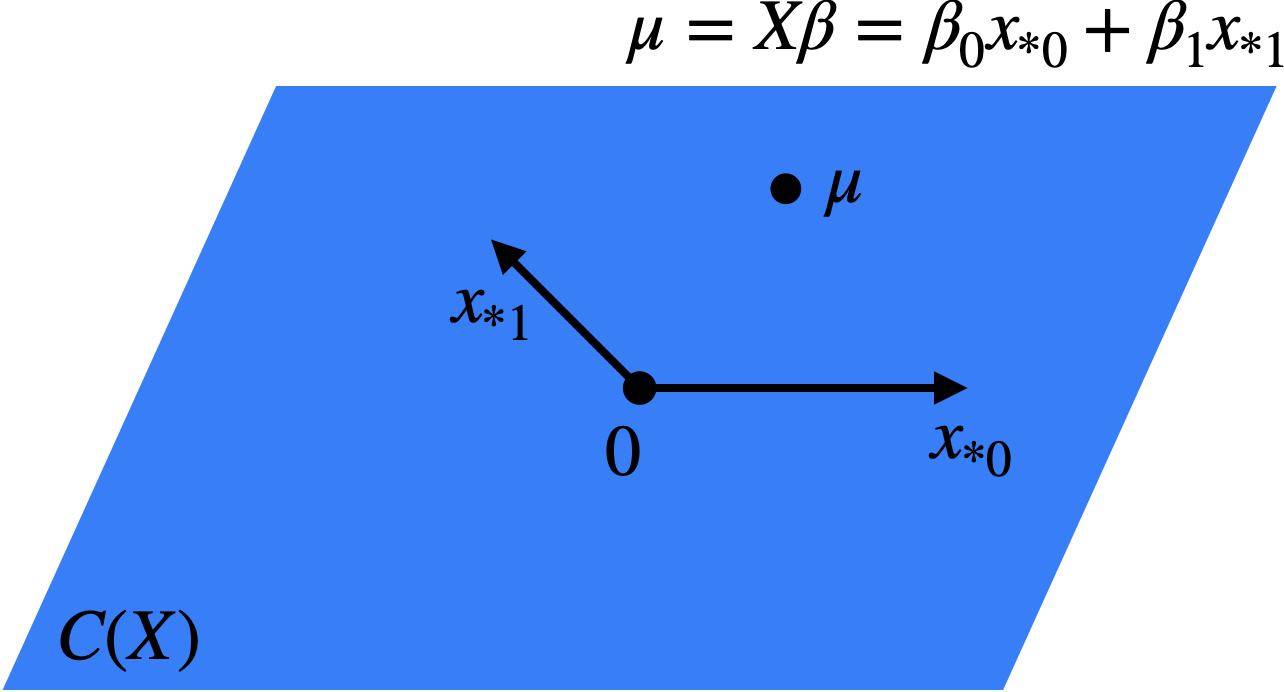
\includegraphics[width=0.5\textwidth,height=\textheight]{figures/model-vector-space.png}

}

\caption{\label{fig-model-vector-space}The model vector space.}

\end{figure}

The \emph{dimension} of \(C(\boldsymbol{X})\) is the rank of
\(\boldsymbol{X}\), i.e.~the number of linearly independent columns of
\(\boldsymbol{X}\). If \(\text{rank}(\boldsymbol{X}) < p\), this means
that there are two different vectors \(\boldsymbol{\beta}\) and
\(\boldsymbol{\beta'}\) such that
\(\boldsymbol{X} \boldsymbol{\beta} = \boldsymbol{X} \boldsymbol{\beta'}\).
Therefore, we have two values of the parameter vector that give the same
model for \(\boldsymbol{y}\). This makes \(\boldsymbol{\beta}\)
\emph{not identifiable}, and makes it impossible to reliably determine
\(\boldsymbol{\beta}\) based on the data. For this reason, we will
generally assume that \(\boldsymbol{\beta}\) is \emph{identifiable},
i.e.~\(\boldsymbol{X} \boldsymbol{\beta} \neq \boldsymbol{X} \boldsymbol{\beta'}\)
if \(\boldsymbol{\beta} \neq \boldsymbol{\beta'}\). This is equivalent
to the assumption that \(\text{rank}(\boldsymbol{X}) = p\). Note that
this cannot hold when \(p > n\), so for the majority of the course we
will assume that \(p \leq n\). In this case,
\(\text{rank}(\boldsymbol{X}) = p\) if and only if \(\boldsymbol{X}\)
has \emph{full-rank}.

As an example when \(p \leq n\) but when \(\boldsymbol{\beta}\) is still
not identifiable, consider the case of a categorical predictor. Suppose
the categories of \(w\) were \(\{w_1, \dots, w_{C-1}\}\), i.e.~the
baseline category \(w_0\) did not exist. In this case, the model
(\ref{eq-C-sample-model}) would not be identifiable because
\(x_0 = 1 = x_1 + \cdots + x_{C-1}\) and thus
\(x_{*0} = 1 = x_{*1} + \cdots + x_{*,C-1}\). Indeed, this means that
one of the predictors can be expressed as a linear combination of the
others, so \(\boldsymbol{X}\) cannot have full rank. A simpler way of
phrasing the problem is that we are describing \(C-1\) intrinsic
parameters (the means in each of the \(C-1\) groups) with \(C\) model
parameters. There must therefore be some redundancy. For this reason, if
we include an intercept term in the model then we must designate one of
our categories as the baseline and exclude its indicator from the model.

\hypertarget{sec-least-squares-estimation}{%
\chapter{Least squares estimation}\label{sec-least-squares-estimation}}

\hypertarget{algebraic-perspective}{%
\section{Algebraic perspective}\label{algebraic-perspective}}

\emph{See also Agresti 2.1.1, Dunn and Smyth 2.4.1, 2.5.2}

Now, suppose that we are given a dataset
\((\boldsymbol{X}, \boldsymbol{y})\). How do we go about estimating
\(\boldsymbol{\beta}\) based on this data? The canonical approach is the
\emph{method of least squares}: \[
\boldsymbol{\widehat{\beta}} \equiv \underset{\boldsymbol{\beta}}{\arg \min}\ \|\boldsymbol{y} - \boldsymbol{X} \boldsymbol{\beta}\|^2.
\] The quantity \[
\|\boldsymbol{y} - \boldsymbol{X} \boldsymbol{\widehat{\beta}}\|^2 = \|\boldsymbol{y} - \boldsymbol{\widehat{\mu}}\|^2 = \sum_{i = 1}^n (y_i - \widehat{\mu}_i)^2
\] is called the \emph{residual sum of squares (RSS)}, and it measures
the lack of fit of the linear regression model. We therefore want to
choose \(\boldsymbol{\widehat{\beta}}\) to minimize this lack of fit.
Letting
\(L(\boldsymbol{\beta}) = \frac{1}{2}\|\boldsymbol{y} - \boldsymbol{X} \boldsymbol{\beta}\|^2\),
we can do some calculus to derive that \[
\frac{\partial}{\partial \boldsymbol{\beta}}L(\boldsymbol{\beta}) = -\boldsymbol{X}^T(\boldsymbol{y} - \boldsymbol{X} \boldsymbol{\beta}).
\] Setting this vector of partial derivatives equal to zero, we arrive
at the \emph{normal equations}:
\begin{equation}\protect\hypertarget{eq-normal-equations}{}{
-\boldsymbol{X}^T(\boldsymbol{y} - \boldsymbol{X} \boldsymbol{\widehat{\beta}}) = 0 \quad \Longleftrightarrow \quad \boldsymbol{X}^T \boldsymbol{X} \boldsymbol{\widehat{\beta}} = \boldsymbol{X}^T \boldsymbol{y}.
}\label{eq-normal-equations}\end{equation} If \(\boldsymbol{X}\) is full
rank, the matrix \(\boldsymbol{X}^T \boldsymbol{X}\) is invertible and
we can therefore conclude that
\begin{equation}\protect\hypertarget{eq-beta-hat}{}{
\boldsymbol{\widehat{\beta}} = (\boldsymbol{X}^T \boldsymbol{X})^{-1}\boldsymbol{X}^T \boldsymbol{y}.
}\label{eq-beta-hat}\end{equation}

\hypertarget{probabilistic-perspective}{%
\section{Probabilistic perspective}\label{probabilistic-perspective}}

\emph{See also Agresti 2.7.1}

\hypertarget{least-squares-as-maximum-likelihood-estimation}{%
\subsection{Least squares as maximum likelihood
estimation}\label{least-squares-as-maximum-likelihood-estimation}}

Note that if \(\boldsymbol{\epsilon}\) is assumed to be
\(N(0,\sigma^2 \boldsymbol{I_n})\), then the least squares solution
would also be the maximum likelihood solution. Indeed, for
\(y_i \sim N(\mu_i, \sigma^2)\), the log-likelihood is:

\[
\log \left[\prod_{i = 1}^n \frac{1}{\sqrt{2\pi\sigma^2}}\exp\left(-\frac{(y_i - \mu_i)^2}{2\sigma^2}\right)\right] = \text{constant} - \frac{1}{2\sigma^2}\sum_{i = 1}^n (y_i - \mu_i)^2.
\]

\hypertarget{gauss-markov-theorem}{%
\subsection{Gauss-Markov theorem}\label{gauss-markov-theorem}}

Now that we have derived the least squares estimator, we can compute its
bias and variance. To obtain the bias, we first calculate that:

\[
\mathbb{E}[\widehat{\boldsymbol{\beta}}] = \mathbb{E}[(\boldsymbol{X}^T \boldsymbol{X})^{-1}\boldsymbol{X}^T \boldsymbol{y}] = (\boldsymbol{X}^T \boldsymbol{X})^{-1}\boldsymbol{X}^T \mathbb{E}[\boldsymbol{y}] = (\boldsymbol{X}^T \boldsymbol{X})^{-1}\boldsymbol{X}^T \boldsymbol{X} \boldsymbol{\beta} = \boldsymbol{\beta}.
\]

Therefore, the least squares estimator is unbiased. To obtain the
variance, we compute:

\begin{equation}\protect\hypertarget{eq-var-of-beta-hat}{}{
\begin{split}
\text{Var}[\boldsymbol{\widehat{\beta}}] &= \text{Var}[(\boldsymbol{X}^T \boldsymbol{X})^{-1}\boldsymbol{X}^T \boldsymbol{y}] \\
&= (\boldsymbol{X}^T \boldsymbol{X})^{-1}\boldsymbol{X}^T\text{Var}[\boldsymbol{y}]\boldsymbol{X} (\boldsymbol{X}^T \boldsymbol{X})^{-1} \\
&= (\boldsymbol{X}^T \boldsymbol{X})^{-1}\boldsymbol{X}^T(\sigma^2 \boldsymbol{I_n})\boldsymbol{X} (\boldsymbol{X}^T \boldsymbol{X})^{-1} \\
&= \sigma^2 (\boldsymbol{X}^T \boldsymbol{X})^{-1}.
\end{split}
}\label{eq-var-of-beta-hat}\end{equation}

\begin{theorem}[Gauss-Markov
theorem]\protect\hypertarget{thm-gauss-markov}{}\label{thm-gauss-markov}

For homoskedastic linear models (eqs. (\ref{eq-lm1}) and
(\ref{eq-lm2})), the least squares coefficient estimates have the
smallest covariance matrix (in the sense of positive semidefinite
matrices) among all linear unbiased estimates of \(\boldsymbol{\beta}\).

\end{theorem}

\hypertarget{geometric-perspective}{%
\section{Geometric perspective}\label{geometric-perspective}}

\emph{See also Agresti 2.2.1-2.2.3}

The following is the key geometric property of least squares
(Figure~\ref{fig-least-squares-as-projection}).

\begin{proposition}[]\protect\hypertarget{prp-orthogonal-projection}{}\label{prp-orthogonal-projection}

The mapping
\(\boldsymbol{y} \mapsto \boldsymbol{\widehat{\mu}} = \boldsymbol{X}\boldsymbol{\widehat{\beta}} \in C(\boldsymbol{X})\)
is an \emph{orthogonal projection} onto \(C(\boldsymbol{X})\), with
projection matrix

\begin{equation}\protect\hypertarget{eq-hat-matrix}{}{
\boldsymbol{H} \equiv  \boldsymbol{X}(\boldsymbol{X}^T \boldsymbol{X})^{-1}\boldsymbol{X}^T \quad (\textit{the hat matrix}).
}\label{eq-hat-matrix}\end{equation}

\end{proposition}

Geometrically, this makes sense since we define
\(\boldsymbol{\widehat{\beta}}\) so that
\(\boldsymbol{\widehat{\mu}} \in C(\boldsymbol{X})\) is as close to
\(\boldsymbol{y}\) as possible. The shortest path between a point and a
plane is the perpendicular. A simple example of \(\boldsymbol{H}\) can
be obtained by considering the intercept-only regression.

\begin{proof}

To prove that \(\boldsymbol{y} \mapsto \boldsymbol{\widehat{\mu}}\) is
an orthogonal projection onto \(C(\boldsymbol{X})\), it suffices to show
that:

\[
\boldsymbol{v}^T (\boldsymbol{y} - \boldsymbol{X} \boldsymbol{\widehat{\beta}}) = 0 \text{ for each } \boldsymbol{v} \in C(\boldsymbol{X}).
\]

Since the columns
\(\{\boldsymbol{x_{*0}}, \dots, \boldsymbol{x_{*p-1}}\}\) of
\(\boldsymbol{X}\) form a basis for \(C(\boldsymbol{X})\), it suffices
to show that
\(\boldsymbol{x_{*j}}^T (\boldsymbol{y} - \boldsymbol{X} \boldsymbol{\widehat{\beta}}) = 0\)
for each \(j = 0, \dots, p-1\). This is a consequence of the normal
equations
\(\boldsymbol{X}^T(\boldsymbol{y} - \boldsymbol{X}\boldsymbol{\widehat{\beta}}) = 0\)
derived in (\ref{eq-normal-equations}).

To show that the projection matrix is \(\boldsymbol{H}\)
(\ref{eq-hat-matrix}), it suffices to check that:

\[
\boldsymbol{\widehat{\mu}} = \boldsymbol{X}\boldsymbol{\widehat{\beta}} = \boldsymbol{X}(\boldsymbol{X}^T \boldsymbol{X})^{-1}\boldsymbol{X}^T \boldsymbol{y} \equiv \boldsymbol{H} \boldsymbol{y}.
\]

\end{proof}

\begin{figure}

{\centering 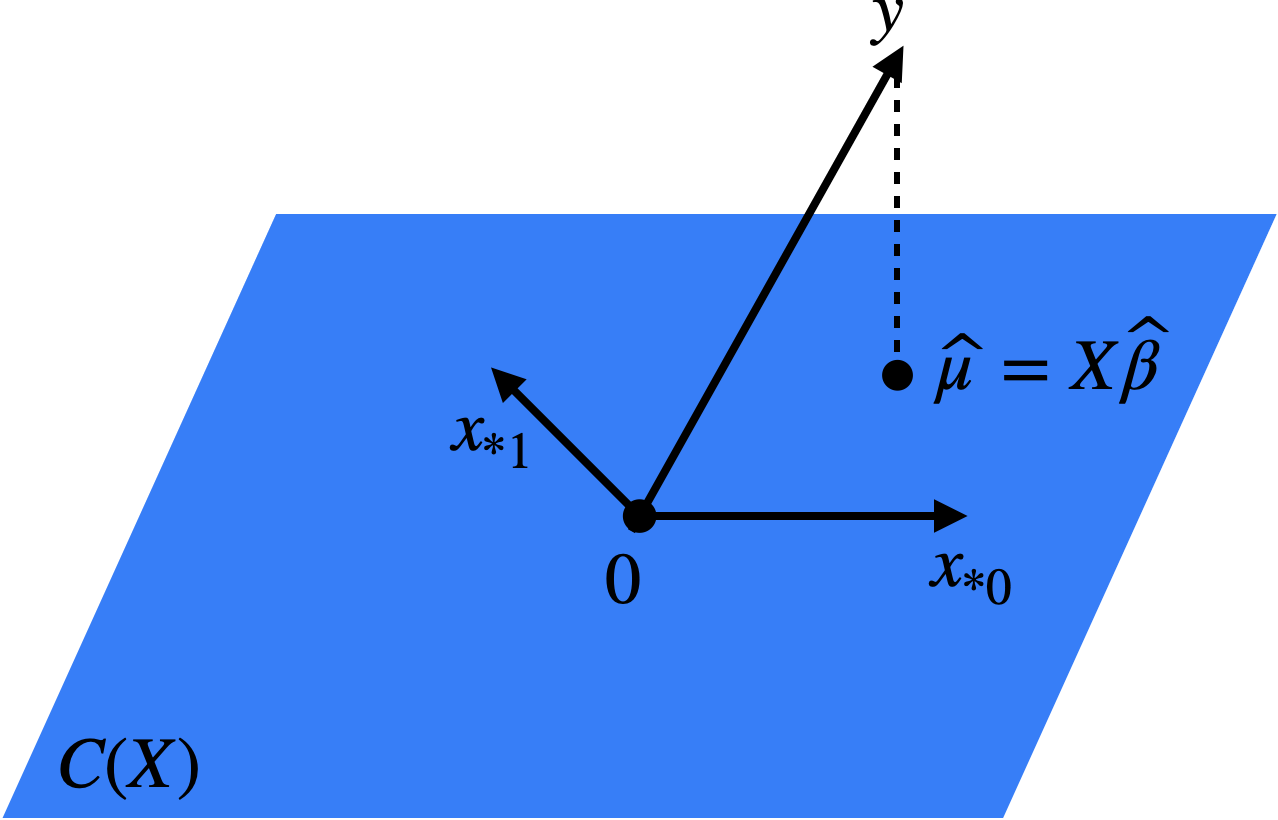
\includegraphics[width=0.5\textwidth,height=\textheight]{figures/least-squares-as-projection.png}

}

\caption{\label{fig-least-squares-as-projection}Least squares as
orthogonal projection.}

\end{figure}

\begin{proposition}[]\protect\hypertarget{prp-projection-matrices}{}\label{prp-projection-matrices}

If \(\boldsymbol{P}\) is an orthogonal projection onto a subspace
\(\boldsymbol{W}\), then:

\begin{enumerate}
\def\labelenumi{\arabic{enumi}.}
\tightlist
\item
  \(\boldsymbol{P}\) is idempotent, i.e.,
  \(\boldsymbol{P}^2 = \boldsymbol{P}\).
\item
  For all \(\boldsymbol{v} \in \boldsymbol{W}\), we have
  \(\boldsymbol{P}\boldsymbol{v} = \boldsymbol{v}\), and for all
  \(\boldsymbol{v} \in \boldsymbol{W}^{\perp}\), we have
  \(\boldsymbol{P} \boldsymbol{v} = 0\).
\item
  \(\text{trace}(\boldsymbol{P}) = \text{dim}(\boldsymbol{W})\).
\end{enumerate}

\end{proposition}

One consequence of the geometric interpretation of least squares is that
the fitted values \(\boldsymbol{\widehat{\mu}}\) depend on
\(\boldsymbol{X}\) only through \(C(\boldsymbol{X})\). As we will see in
Homework 1, there are many different model matrices \(\boldsymbol{X}\)
leading to the same model space. Essentially, this reflects the fact
that there are many different bases for the same vector space. Consider,
for example, changing the units on the columns of \(\boldsymbol{X}\). It
can be verified that not just the fitted values
\(\boldsymbol{\widehat{\mu}}\) but also the predictions on a new set of
features remain invariant to reparametrization (this follows from parts
(a) and (b) of Homework 1 Problem 1). Therefore, while reparametrization
can have a huge impact on the fitted coefficients, it has no impact on
the predictions of linear regression.

\hypertarget{sec-anova}{%
\chapter{Analysis of variance}\label{sec-anova}}

\emph{See also Agresti 2.4.2, 2.4.3, 2.4.6, Dunn and Smyth 2.9}

\hypertarget{analysis-of-variance}{%
\section{Analysis of variance}\label{analysis-of-variance}}

The orthogonality property of least squares, together with the
Pythagorean theorem, leads to a fundamental relationship called
\emph{the analysis of variance}.

Let's say that \(S \subset \{0, 1, \dots, p-1\}\) is a subset of the
predictors we wish to exclude from the model. First regress
\(\boldsymbol{y}\) on \(\boldsymbol{X}\) to get
\(\boldsymbol{\widehat{\beta}}\) as usual. Then, we consider the
\emph{partial model matrix} \(\boldsymbol{X_{*,\text{-}S}}\) obtained by
selecting all predictors except those in \(S\). Regressing
\(\boldsymbol{y}\) on \(\boldsymbol{X_{*, \text{-}S}}\) results in
\(\boldsymbol{\widehat{\beta}_{\text{-}S}}\) (note:
\(\boldsymbol{\widehat{\beta}_{\text{-}S}}\) is not necessarily obtained
from \(\boldsymbol{\widehat{\beta}}\) by extracting the coefficients
corresponding to \(\text{-}S\)).

\begin{theorem}[]\protect\hypertarget{thm-analysis-of-variance}{}\label{thm-analysis-of-variance}

\begin{equation}\protect\hypertarget{eq-pythagorean-theorem}{}{
\|\boldsymbol{y} -  \boldsymbol{X_{*, \text{-}S}}\boldsymbol{\widehat{\beta}_{\text{-}S}}\|^2 = \|\boldsymbol{X}\boldsymbol{\widehat{\beta}} - \boldsymbol{X_{*, \text{-}S}}\boldsymbol{\widehat{\beta}_{\text{-}S}}\|^2 + \|\boldsymbol{y} - \boldsymbol{X}\boldsymbol{\widehat{\beta}}\|^2.
}\label{eq-pythagorean-theorem}\end{equation}

\end{theorem}

\begin{proof}

Consider the three points \(\boldsymbol{y}\),
\(\boldsymbol{X}\boldsymbol{\widehat{\beta}}\),
\(\boldsymbol{X_{*, \text{-}S}}\boldsymbol{\widehat{\beta}_{\text{-}S}} \in \mathbb{R}^n\).
Since \(\boldsymbol{X}\boldsymbol{\widehat{\beta}}\) and
\(\boldsymbol{X_{*, \text{-}S}}\boldsymbol{\widehat{\beta}_{\text{-}S}}\)
are both in \(C(\boldsymbol{X})\), it follows by the orthogonal
projection property that
\(\boldsymbol{y} - \boldsymbol{X}\boldsymbol{\widehat{\beta}}\) is
orthogonal to
\(\boldsymbol{X}\boldsymbol{\widehat{\beta}} - \boldsymbol{X_{*, \text{-}S}}\boldsymbol{\widehat{\beta}_{\text{-}S}}\).
In other words, these three points form a right triangle
(Figure~\ref{fig-sum-of-squares}). The relationship
(\ref{eq-pythagorean-theorem}) is then a consequence of the Pythagorean
theorem.

\end{proof}

\begin{figure}

{\centering 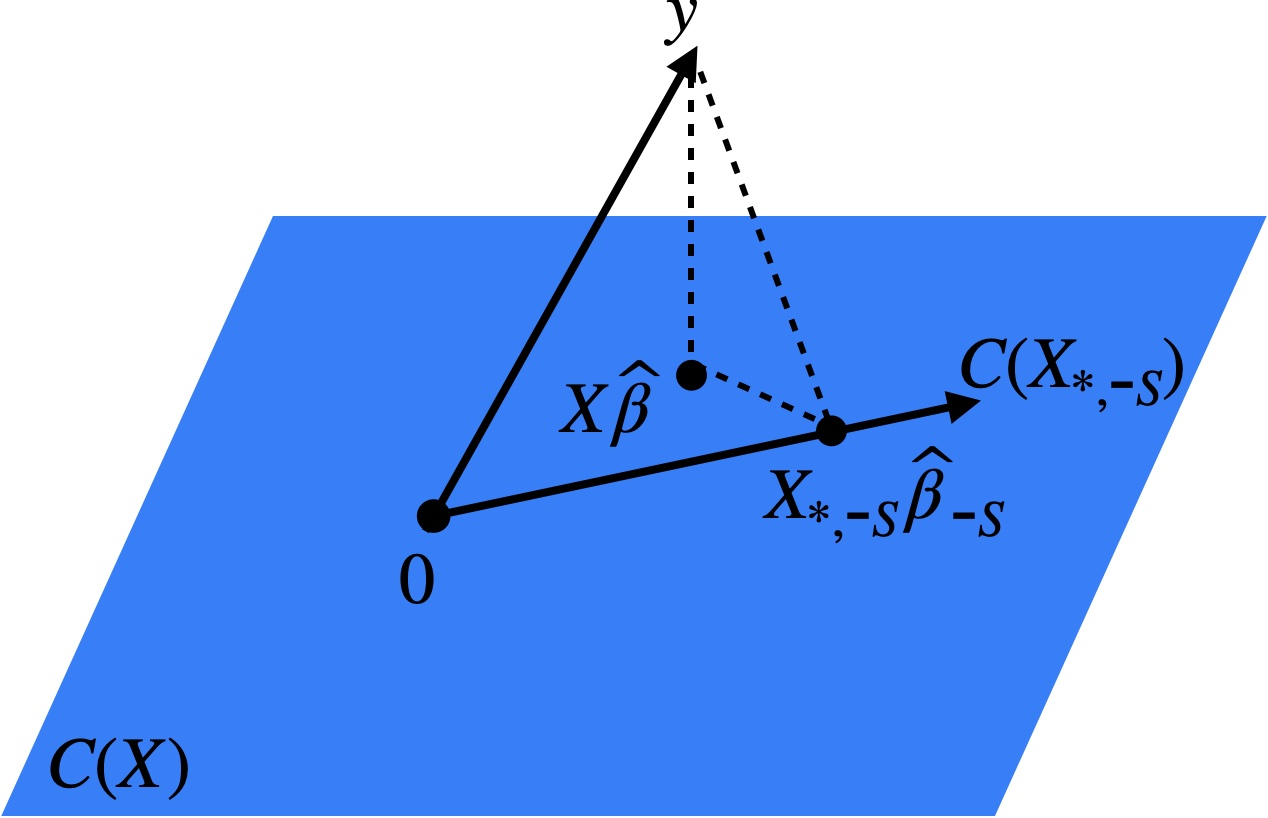
\includegraphics[width=0.5\textwidth,height=\textheight]{figures/sum-of-squares.jpeg}

}

\caption{\label{fig-sum-of-squares}Pythagorean theorem for regression on
a subset of predictors.}

\end{figure}

We will rely on this fundamental relationship throughout this course.
One important special case is when \(S = \{1, \dots, p-1\}\), i.e., the
model without \(S\) is the intercept-only model. In this case,
\(\boldsymbol{X_{*, \text{-}S}} = \boldsymbol{1_n}\) and
\(\boldsymbol{\widehat{\beta}_{\text{-}S}} = \bar{y}\). Therefore,
equation (\ref{eq-pythagorean-theorem}) implies the following.

\begin{proposition}[]\protect\hypertarget{prp-sum-of-squares}{}\label{prp-sum-of-squares}

\[
\|\boldsymbol{y} -  \bar{y} \boldsymbol{1_n}\|^2 = \|\boldsymbol{X}\boldsymbol{\widehat{\beta}} - \bar{y} \boldsymbol{1_n}\|^2 + \|\boldsymbol{y} - \boldsymbol{X}\boldsymbol{\widehat{\beta}}\|^2.
\]

Equivalently, we can rewrite this equation as follows:

\begin{equation}\protect\hypertarget{eq-anova}{}{
\textnormal{SST} \equiv \sum_{i = 1}^n (y_i - \bar{y})^2 = \sum_{i = 1}^n (\widehat{\mu}_i - \bar{y})^2 + \sum_{i = 1}^n (y_i - \widehat{\mu}_i)^2 \equiv \textnormal{SSR} + \textnormal{SSE}.
}\label{eq-anova}\end{equation}

\end{proposition}

\hypertarget{r2-and-multiple-correlation}{%
\section{\texorpdfstring{\(R^2\) and multiple
correlation}{R\^{}2 and multiple correlation}}\label{r2-and-multiple-correlation}}

The ANOVA decomposition (\ref{eq-anova}) of the variation in
\(\boldsymbol{y}\) into that explained by the linear regression model
(SSR) and that left over (SSE) leads naturally to the definition of
\(R^2\) as the fraction of variation in \(\boldsymbol{y}\) explained by
the linear regression model:

\[
R^2 \equiv \frac{\text{SSR}}{\text{SST}} = \frac{\sum_{i = 1}^n (\widehat{\mu}_i - \bar{y})^2}{\sum_{i = 1}^n (y_i - \bar{y})^2} = \frac{\|\boldsymbol{X}\boldsymbol{\widehat{\beta}} - \bar{y} \boldsymbol{1_n}\|^2}{\|\boldsymbol{y} -  \bar{y} \boldsymbol{1_n}\|^2}.
\]

By the decomposition (\ref{eq-anova}), we have \(R^2 \in [0,1]\). The
closer \(R^2\) is to 1, the more closely the data follow the fitted
linear regression model. This intuition is formalized in the following
result.

\begin{proposition}[]\protect\hypertarget{prp-multiple-correlation}{}\label{prp-multiple-correlation}

\(R^2\) is the squared sample correlation between
\(\boldsymbol{X} \boldsymbol{\widehat{\beta}}\) and \(\boldsymbol{y}\).

\end{proposition}

For this reason, the positive square root of \(R^2\) is called the
\emph{multiple correlation coefficient}.

\begin{proof}

The first step is to observe that the mean of
\(\boldsymbol{X} \boldsymbol{\widehat{\beta}}\) is \(\bar{y}\) (this
follows from the normal equations). Therefore, the sample correlation
between \(\boldsymbol{X} \boldsymbol{\widehat{\beta}}\) and
\(\boldsymbol{y}\) is the inner product of the unit-normalized vectors
\(\boldsymbol{X} \boldsymbol{\widehat{\beta}} - \bar{y} \boldsymbol{1}\)
and \(\boldsymbol{y} - \bar{y} \boldsymbol{1}\), which is the cosine of
the angle between them. From the geometry of
Figure~\ref{fig-sum-of-squares}, we find that the cosine of the angle
between
\(\boldsymbol{X} \boldsymbol{\widehat{\beta}} - \bar{y} \boldsymbol{1}\)
and \(\boldsymbol{y} - \bar{y} \boldsymbol{1}\) is
\(\|\boldsymbol{X} \boldsymbol{\widehat{\beta}} - \bar{y} \boldsymbol{1}\|/\|\boldsymbol{y} - \bar{y} \boldsymbol{1}\|\).
Squaring this relation gives the desired conclusion.

\end{proof}

\hypertarget{r2-increases-as-predictors-are-added}{%
\section{\texorpdfstring{\(R^2\) increases as predictors are
added}{R\^{}2 increases as predictors are added}}\label{r2-increases-as-predictors-are-added}}

The \(R^2\) is an \emph{in-sample} measure, i.e., it uses the same data
to fit the model and to assess the quality of the fit. Therefore, it is
generally an optimistic measure of the (out-of-sample) prediction error.
One manifestation of this is that the \(R^2\) increases if any
predictors are added to the model (even if these predictors are
``junk''). To see this, it suffices to show that SSE decreases as we add
predictors. Without loss of generality, suppose that we start with a
model with all predictors except those in
\(S \subset \{0, 1, \dots, p-1\}\) and compare it to the model including
all the predictors \(\{0,1,\dots,p-1\}\). We can read off from the
Pythagorean theorem (\ref{eq-pythagorean-theorem}) that:

\[
\text{SSE}(\boldsymbol{X_{*, \text{-}S}}, \boldsymbol{y}) \equiv \|\boldsymbol{y} -  \boldsymbol{X_{*, \text{-}S}}\boldsymbol{\widehat{\beta}_{\text{-}S}}\|^2 \geq  \|\boldsymbol{y} -  \boldsymbol{X}\boldsymbol{\widehat{\beta}}\|^2 \equiv \text{SSE}(\boldsymbol{X}, \boldsymbol{y}).
\]

Adding many junk predictors will have the effect of degrading predictive
performance but will nevertheless increase \(R^2\).

\hypertarget{special-cases}{%
\section{Special cases}\label{special-cases}}

\hypertarget{the-c-groups-model}{%
\subsection{\texorpdfstring{The \(C\)-groups
model}{The C-groups model}}\label{the-c-groups-model}}

\emph{See also Agresti 2.3.2-2.3.3}

\hypertarget{anova-decomposition-for-c-groups-model}{%
\subsubsection{\texorpdfstring{ANOVA decomposition for \(C\) groups
model}{ANOVA decomposition for C groups model}}\label{anova-decomposition-for-c-groups-model}}

Let's consider the special case of the ANOVA decomposition
(\ref{eq-anova}) when the model matrix \(\boldsymbol{X}\) represents a
single categorical predictor \(w\). In this case, each observation \(i\)
is associated with one of the \(C\) classes of \(w\), which we denote
\(c(i) \in \{1, \dots, C\}\). Let's consider the \(C\) groups of
observations \(\{i: c(i) = c\}\) for \(c \in \{1, \dots, C\}\). For
example, \(w\) may be the type of a car (compact, midsize, minivan,
etc.) and \(y\) might be its fuel efficiency in miles per gallon.

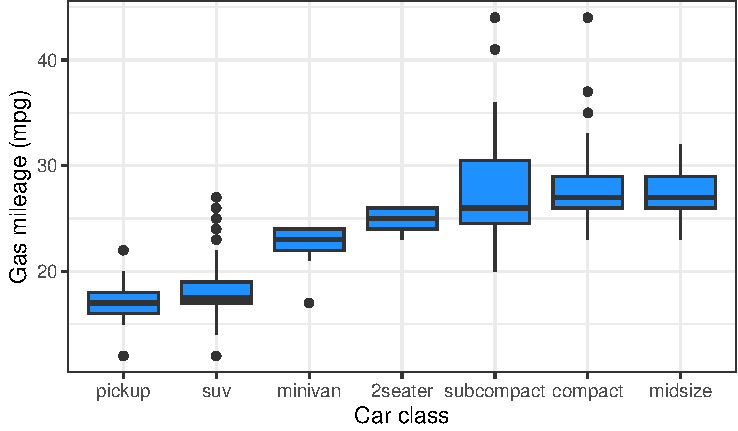
\includegraphics{anova_files/figure-pdf/unnamed-chunk-2-1.pdf}

It is easy to check that the least squares fitted values
\(\widehat{\mu}_i\) are simply the means of the corresponding groups:

\[
\widehat{\mu}_i = \bar{y}_{c(i)}, \quad \text{where}\ \bar{y}_{c(i)} \equiv \frac{\sum_{i: c(i) = c} y_i}{|\{i: c(i) = c\}|}.
\]

Therefore, we have:

\[
\text{SSR} = \sum_{i = 1}^n (\widehat{\mu}_i - \bar{y})^2 = \sum_{i = 1}^n (\bar{y}_{c(i)} - \bar{y})^2 \equiv \text{between-groups sum of squares (SSB)}.
\]

and

\[
\text{SSE} = \sum_{i = 1}^n (y_i - \widehat{\mu}_i)^2 = \sum_{i = 1}^n (y_i - \bar{y}_{c(i)})^2 \equiv \text{within-groups sum of squares (SSW)}.
\]

We therefore obtain the following corollary of the ANOVA decomposition
(\ref{eq-anova}):

\begin{equation}\protect\hypertarget{eq-anova-C-groups}{}{
\text{SST} = \text{SSB} + \text{SSW}.
}\label{eq-anova-C-groups}\end{equation}

\hypertarget{simple-linear-regression}{%
\subsection{Simple linear regression}\label{simple-linear-regression}}

\emph{See also Agresti 2.1.3}

Consider a linear regression model with an intercept and one
quantitative predictor, \(x\):

\begin{equation}\protect\hypertarget{eq-simple-regression}{}{
y = \beta_0 + \beta_1 x + \epsilon.
}\label{eq-simple-regression}\end{equation}

This is the simple linear regression model. In this case, we can compute
that
\begin{equation}\protect\hypertarget{eq-beta1-simple-linear-regression}{}{
\widehat \beta_1 = \frac{\sigma_y}{\sigma_x} \rho_{xy},
}\label{eq-beta1-simple-linear-regression}\end{equation} where
\(\rho_{xy}\) is the sample correlation between \(x\) and \(y\),
\(\sigma^2_x\) is the sample variance of \(x\), and \(\sigma^2_y\) is
the sample variance of \(y\). Furthermore, we have
\begin{equation}\protect\hypertarget{eq-beta0-simple-linear-regression}{}{
\widehat \beta_0 = \bar y - \widehat \beta_1 \bar x.
}\label{eq-beta0-simple-linear-regression}\end{equation}

\hypertarget{anova-decomposition-for-simple-linear-regression}{%
\subsubsection{ANOVA decomposition for simple linear
regression}\label{anova-decomposition-for-simple-linear-regression}}

Figure~\ref{fig-anova-simple-linear-regression} gives an interpretation
of the ANOVA decomposition (\ref{eq-anova}) in the case of the simple
linear regression model (\ref{eq-simple-regression}).

\begin{figure}

{\centering 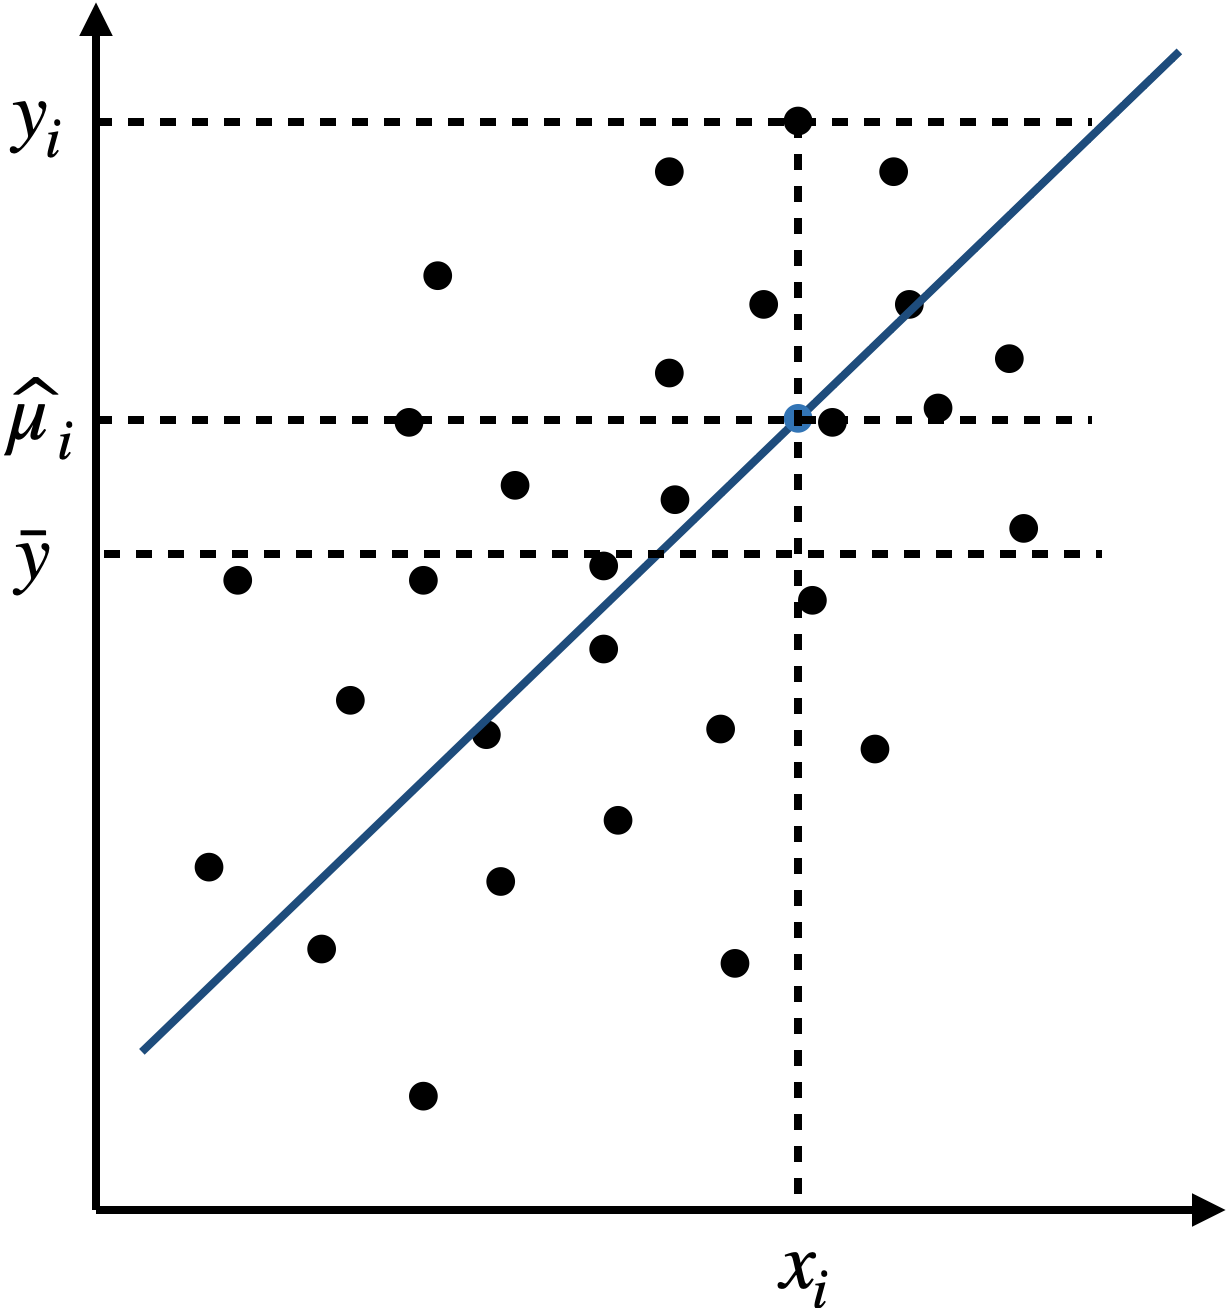
\includegraphics[width=0.4\textwidth,height=\textheight]{figures/anova-simple-linear-regression.png}

}

\caption{\label{fig-anova-simple-linear-regression}ANOVA decomposition
for simple linear regression.}

\end{figure}

\hypertarget{connection-between-r2-and-correlation}{%
\subsubsection{\texorpdfstring{Connection between \(R^2\) and
correlation}{Connection between R\^{}2 and correlation}}\label{connection-between-r2-and-correlation}}

There is a connection between \(R^2\) and correlation in simple linear
regression.

\begin{proposition}[]\protect\hypertarget{prp-R2-correlation}{}\label{prp-R2-correlation}

Let \(\rho_{xy}\) denote the sample correlation between \(x\) and \(y\),
and let \(R^2_{xy}\) be the \(R^2\) from the simple linear regression
(\ref{eq-simple-regression}). Then, we have: \[
R^2 = \rho_{xy}^2.
\]

\end{proposition}

\begin{proof}

This fact is a consequence of
Proposition~\ref{prp-multiple-correlation}.

\end{proof}

\hypertarget{regression-to-the-mean}{%
\subsubsection{Regression to the mean}\label{regression-to-the-mean}}

Simple linear regression can be used to study the relationship between
the same quantity across time (or generations). For example, let \(x\)
and \(y\) be the height of a parent and child. This example motivated
Sir Francis Galton to study linear regression in the first place.
Alternatively, \(x\) and \(y\) can be a student's score on a
standardized test in two consecutive years, or the number of games won
by a given sports team in two consecutive seasons. In this situation, it
is reasonable to assume that the sample standard deviations of \(x\) and
\(y\) are the same (or to normalize these variables to achieve this). In
this case, equations (\ref{eq-beta1-simple-linear-regression}) and
(\ref{eq-beta0-simple-linear-regression}) simplify to:

\begin{equation}\protect\hypertarget{eq-coefficient-as-correlation}{}{
\widehat{\beta}_0 = \bar{y} - \rho_{xy} \bar{x} \quad \text{and} \quad \widehat{\beta}_1 = \rho_{xy}.
}\label{eq-coefficient-as-correlation}\end{equation}

It follows that:

\[
|\widehat{\mu}_i - \bar{y}| = |\widehat{\beta}_0 + \widehat{\beta}_1 x_i - \bar{y}| = |\rho_{xy}(x_i - \bar{x})| = |\rho_{xy}| \cdot |x_i - \bar{x}|.
\]

Since \(|\rho_{xy}| < 1\) unless \(\boldsymbol{x}\) and
\(\boldsymbol{y}\) are perfectly correlated (by the Cauchy-Schwarz
inequality), this means that:

\begin{equation}\protect\hypertarget{eq-regression-to-the-mean}{}{
|\widehat{\mu}_i - \bar{y}| < |x_i - \bar{x}| \quad \text{for each } i.
}\label{eq-regression-to-the-mean}\end{equation}

Therefore, we expect \(y_i\) to be closer to its mean than \(x_i\) is to
its mean. This phenomenon is called \emph{regression to the mean} (and
is in fact the origin of the term ``regression''). Many mistakenly
attribute a causal mechanism to this phenomenon, when in reality it is
simply a statistical artifact. For example, suppose \(x_i\) is the
number of games a sports team won last season and \(y_i\) is the number
of games it won this season. It is widely observed that teams with
exceptional performance in a given season suffer a ``winner's curse,''
performing worse in the next season. The reason for the winner's curse
is simple: teams perform exceptionally well due to a combination of
skill and luck. While skill stays roughly constant from year to year,
the team which performed exceptionally well in a given season is
unlikely to get as lucky as it did the next season.

\hypertarget{sec-collinearity}{%
\chapter{Collinearity and adjustment}\label{sec-collinearity}}

\emph{See also Agresti 2.2.4, 2.5.6, 2.5.7, 4.6.5}

An important part of linear regression analysis is the dependence of the
least squares coefficient for a predictor (\(x_j\)) on what other
predictors are in the model \((\boldsymbol x_{\text{-}j})\). This
relationship is dictated by the extent to which \(\boldsymbol x_{*j}\)
is correlated with \(\boldsymbol X_{*,\text{-}j}\). To explore this
phenomenon, it will be useful to compare two different regressions:

\begin{itemize}
\tightlist
\item
  Regress \(\boldsymbol y\) on \emph{just} \(\boldsymbol{x}_{*j}\). Let
  the resulting coefficient for \(x_j\) be \(\widehat{\beta}_j\).
\item
  Regress \(\boldsymbol y\) on \emph{all of} \(\boldsymbol X\) (i.e., on
  both \(\boldsymbol{x}_{*j}\) and \(\boldsymbol X_{*, \text{-}j}\)).
  Let the resulting coefficients for \(x_j\) and
  \(\boldsymbol x_{\text{-}j}\) be \(\widehat{\beta}_{j|\text{-}j}\) and
  \(\widehat{\beta}_{\text{-}j|j}\), respectively.
\end{itemize}

\hypertarget{least-squares-estimates-in-the-orthogonal-case}{%
\section{Least squares estimates in the orthogonal
case}\label{least-squares-estimates-in-the-orthogonal-case}}

The simplest case to analyze is when \(\boldsymbol x_{*j}\) is
orthogonal to \(\boldsymbol X_{*,\text{-}j}\) in the sense that

\begin{equation}\protect\hypertarget{eq-orthogonality-assumption}{}{
\boldsymbol x_{*j}^T \boldsymbol X_{*,\text{-}j} = \boldsymbol{0}.
}\label{eq-orthogonality-assumption}\end{equation}

In this case, we can derive the least squares coefficient vector
\(\boldsymbol{\widehat{\beta}} = (\widehat{\beta}_{j|\text{-}j}, \boldsymbol{\widehat{\beta}}_{\text{-}j|j})\)
in the regression of \(\boldsymbol y\) on \(\boldsymbol X\):

\begin{equation}\protect\hypertarget{eq-orthogonality}{}{
\begin{split}
\begin{pmatrix}
\widehat{\beta}_{j|\text{-}j} \\
\boldsymbol{\widehat{\beta}}_{\text{-}j|j}
\end{pmatrix} &= (\boldsymbol{X}^T \boldsymbol{X})^{-1} \boldsymbol{X}^T \boldsymbol{y} \\
&=
\begin{pmatrix}
\boldsymbol x_{*j}^T \boldsymbol x_{*j} & \boldsymbol{0} \\
\boldsymbol{0} & \boldsymbol{X}_{*,\text{-}j}^T \boldsymbol{X}_{*,\text{-}j}
\end{pmatrix}^{-1}
\begin{pmatrix}
\boldsymbol x_{*j}^T \\
\boldsymbol{X}_{*,\text{-}j}^T
\end{pmatrix} \boldsymbol{y} \\
&=
\begin{pmatrix}
(\boldsymbol x_{*j}^T \boldsymbol x_{*j})^{-1} \boldsymbol x_{*j}^T \boldsymbol{y} \\
(\boldsymbol{X}_{*,\text{-}j}^T \boldsymbol{X}_{*,\text{-}j})^{-1} \boldsymbol{X}_{*,\text{-}j}^T \boldsymbol{y}
\end{pmatrix} \\
&= 
\begin{pmatrix}
\widehat{\beta}_{j} \\
\boldsymbol{\widehat{\beta}}_{\text{-}j}
\end{pmatrix}.
\end{split}
}\label{eq-orthogonality}\end{equation}

Therefore, the least squares coefficient of \(x_j\) is the same
regardless of whether the other predictors are included in the
regression, i.e.

\begin{equation}\protect\hypertarget{eq-orthogonality-consequence}{}{
\widehat{\beta}_{j|\text{-}j} = \widehat{\beta}_{j}.
}\label{eq-orthogonality-consequence}\end{equation}

\hypertarget{least-squares-estimates-via-orthogonalization}{%
\section{Least squares estimates via
orthogonalization}\label{least-squares-estimates-via-orthogonalization}}

The orthogonality assumption (\ref{eq-orthogonality-assumption}) is
almost never satisfied in practice. Usually, \(\boldsymbol{x}_{*j}\) has
a nonzero projection
\(\boldsymbol{X}_{*,\text{-}j}\boldsymbol{\widehat{\gamma}}\) onto
\(C(\boldsymbol{X}_{*,\text{-}j})\):

\[
\boldsymbol{x}_{*j} = \boldsymbol{X}_{*,\text{-}j}\boldsymbol{\widehat{\gamma}} + \boldsymbol{x}^{\perp}_{*j},
\]

where \(\boldsymbol{x}^{\perp}_{*j}\) is the residual from regressing
\(\boldsymbol{x}_{*j}\) onto \(\boldsymbol{X}_{*,\text{-}j}\) and is
therefore orthogonal to \(C(\boldsymbol{X}_{*,\text{-}j})\). In other
words, \(\boldsymbol{x}^{\perp}_{*j}\) is the projection of
\(\boldsymbol{x}_{*j}\) onto the orthogonal complement of
\(C(\boldsymbol{X}_{*,\text{-}j})\). Another way of framing this
relationship is that \(\boldsymbol{x}^{\perp}_{*j}\) is the result of
\emph{adjusting} \(\boldsymbol{x}_{*j}\) for
\(\boldsymbol{X}_{*,\text{-}j}\).

With this decomposition, let us change basis from
\((\boldsymbol{x}_{*j}, \boldsymbol{X}_{*,\text{-}j})\) to
\((\boldsymbol{x}^{\perp}_{*j}, \boldsymbol{X}_{*,\text{-}j})\) by the
process explored in Homework 1 Question 1. Let us write:

\[
\begin{aligned}
\boldsymbol{y} &= \boldsymbol{x}_{*j} \beta_{j|\text{-}j} + \boldsymbol{X}_{*,\text{-}j}\boldsymbol{\beta}_{\text{-}j|j} + \boldsymbol{\epsilon} \\
&\Longleftrightarrow \ \boldsymbol{y} = (\boldsymbol{X}_{*,\text{-}j}\boldsymbol{\widehat{\gamma}} + \boldsymbol{x}^{\perp}_{*j})\beta_{j|\text{-}j} + \boldsymbol{X}_{*,\text{-}j}\boldsymbol{\beta}_{\text{-}j|j} + \boldsymbol{\epsilon} \\
&\Longleftrightarrow \ \boldsymbol{y} = \boldsymbol{x}^{\perp}_{*j}\beta_{j|\text{-}j} + \boldsymbol{X}_{*,\text{-}j}\boldsymbol{\beta}'_{\text{-}j|j} + \boldsymbol{\epsilon}.
\end{aligned}
\]

What this means is that \(\widehat{\beta}_{j|\text{-}j}\), the least
squares coefficient of \(\boldsymbol{x}_{*j}\) in the regression of
\(\boldsymbol{y}\) on
\((\boldsymbol{x}_{*j}, \boldsymbol{X}_{*,\text{-}j})\), is also the
least squares coefficient of \(\boldsymbol{x}^{\perp}_{*j}\) in the
regression of \(\boldsymbol{y}\) on
\((\boldsymbol{x}^{\perp}_{*j}, \boldsymbol{X}_{*,\text{-}j})\).
However, since \(\boldsymbol{x}^{\perp}_{*j}\) is orthogonal to
\(\boldsymbol{X}_{*,\text{-}j}\) by construction, we can use the result
(\ref{eq-orthogonality}) to conclude that:

\[
\widehat{\beta}_{j|\text{-}j} \text{ is the least squares coefficient of } \boldsymbol{x}^{\perp}_{*j} \text{ in the } \textit{univariate} \text{ regression of } \boldsymbol{y} \text{ on } \boldsymbol{x}^{\perp}_{*j}.
\]

We can solve this univariate regression explicitly to obtain:

\begin{equation}\protect\hypertarget{eq-orthogonal-univariate}{}{
\widehat{\beta}_{j|\text{-}j} = \frac{(\boldsymbol{x}^{\perp}_{*j})^T \boldsymbol{y}}{\|\boldsymbol{x}^{\perp}_{*j}\|^2}.
}\label{eq-orthogonal-univariate}\end{equation}

\hypertarget{adjustment-and-partial-correlation}{%
\section{Adjustment and partial
correlation}\label{adjustment-and-partial-correlation}}

Equivalently, letting \(\boldsymbol{\widehat{\beta}}_{\text{-}j}\) be
the least squares estimate in the regression of \(\boldsymbol{y}\) on
\(\boldsymbol{X}_{*,\text{-}j}\) (note that this is \emph{not} the same
as \(\boldsymbol{\widehat{\beta}}_{\text{-}j|j}\)), we can write:

\[
\widehat{\beta}_{j|\text{-}j} = \frac{(\boldsymbol{x}^{\perp}_{*j})^T(\boldsymbol{y} - \boldsymbol{X}_{*,\text{-}j}\boldsymbol{\widehat{\beta}}_{\text{-}j})}{\|\boldsymbol{x}^{\perp}_{*j}\|^2} \equiv \frac{(\boldsymbol{x}^{\perp}_{*j})^T \boldsymbol y^\perp}{\|\boldsymbol{x}^{\perp}_{*j}\|^2}.
\]

We can interpret this result as follows:

\begin{theorem}[]\protect\hypertarget{thm-frisch-waugh-lovell}{}\label{thm-frisch-waugh-lovell}

The linear regression coefficient \(\widehat{\beta}_{j|\text{-}j}\)
results from first adjusting \(\boldsymbol{y}\) and
\(\boldsymbol{x}_{*j}\) for the effects of all other variables, and then
regressing the residuals from \(\boldsymbol{y}\) onto the residuals from
\(\boldsymbol{x}_{*j}\).

\end{theorem}

In this sense, \emph{the least squares coefficient for a predictor in a
multiple linear regression reflects the effect of the predictor on the
response after controlling for the effects of all other predictors.}

Econometricians calls this the Frisch-Waugh-Lovell (FWL) theorem, to
acknowledge economists Ragnar Frisch and Frederick V. Waugh, who first
derived the result in 1933, and Michael C. Lovell, who later
rediscovered and extended it in 1963. In the statistical literature,
this fact was known at least as early as 1907, when Yule documented it
in his paper ``On the Theory of Correlation for any Number of Variables,
treated by a New System of Notation.''

A related quantity is the \emph{partial correlation} between
\(\boldsymbol{x}_{*j}\) and \(\boldsymbol{y}\) after controlling for
\(\boldsymbol{X}_{*,\text{-}j}\), defined as the empirical correlation
between \(\boldsymbol{x}_{*j}^\perp\) and \(\boldsymbol{y}^\perp\): \[
\rho(\boldsymbol{x}_{*j}, \boldsymbol{y}|\boldsymbol{X}_{*,\text{-}j}) \equiv \frac{(\boldsymbol{x}_{*j}^\perp)^T(\boldsymbol{y}^\perp)}{\|\boldsymbol{x}_{*j}^\perp\| \|\boldsymbol{y}^\perp\|}.
\] We can then connect the least squares coefficient
\(\widehat{\beta}_{j|\text{-}j}\) to this partial correlation: \[
\widehat{\beta}_{j|\text{-}j} = \frac{(\boldsymbol{x}^{\perp}_{*j})^T \boldsymbol y^\perp}{\|\boldsymbol{x}^{\perp}_{*j}\|^2} = \frac{\|\boldsymbol{y}^\perp\|}{\|\boldsymbol{x}_{*j}^\perp\|}\rho(\boldsymbol{x}_{*j}, \boldsymbol{y}|\boldsymbol{X}_{*,\text{-}j}),
\]

in a similar spirit to equation
(\ref{eq-beta1-simple-linear-regression}).

\hypertarget{effects-of-collinearity}{%
\section{Effects of collinearity}\label{effects-of-collinearity}}

Collinearity between a predictor \(x_j\) and the other predictors tends
to make the estimate \(\widehat{\beta}_{j|\text{-}j}\) unstable.
Intuitively, this makes sense because it becomes harder to distinguish
between the effects of predictor \(x_j\) and those of the other
predictors on the response. To find the variance of
\(\widehat{\beta}_{j|\text{-}j}\) for a model matrix \(\boldsymbol{X}\),
we could in principle use the formula (\ref{eq-var-of-beta-hat}).
However, this formula involves the inverse of the matrix
\(\boldsymbol{X}^T \boldsymbol{X}\), which is hard to reason about.
Instead, we can employ the formula (\ref{eq-orthogonal-univariate}) to
calculate directly that:

\begin{equation}\protect\hypertarget{eq-conditional-variance}{}{
\text{Var}[\widehat{\beta}_{j|\text{-}j}] = \frac{\sigma^2}{\|\boldsymbol{x}_{*j}^\perp\|^2}.
}\label{eq-conditional-variance}\end{equation}

We see that the variance of \(\widehat{\beta}_{j|\text{-}j}\) is
inversely proportional to \(\|\boldsymbol{x}_{*j}^\perp\|^2\). This
means that the greater the collinearity, the less of
\(\boldsymbol{x}_{*j}\) is left over after adjusting for
\(\boldsymbol{X}_{*,\text{-}j}\), and the greater the variance of
\(\widehat{\beta}_{j|\text{-}j}\). To quantify the effect of this
adjustment, suppose there were no other predictors other than the
intercept term. Then, we would have:

\[
\text{Var}[\widehat{\beta}_{j|1}] = \frac{\sigma^2}{\|\boldsymbol{x}_{*j}-\bar{x}_j \boldsymbol{1}_n\|^2}.
\]

Therefore, we can rewrite the variance (\ref{eq-conditional-variance})
as:

\begin{equation}\protect\hypertarget{eq-vif}{}{
\begin{split}
\text{Var}[\widehat{\beta}_{j|\text{-}j}] &= \frac{\|\boldsymbol{x}_{*j}-\bar{x}_j \boldsymbol{1}_n\|^2}{\|\boldsymbol{x}_{*j}-\boldsymbol{X}_{*,\text{-}j}\boldsymbol{\widehat{\gamma}}\|^2} \cdot \text{Var}[\widehat{\beta}_{j|1}] \\
&= \frac{1}{1-R_j^2} \cdot \text{Var}[\widehat{\beta}_{j|1}] \equiv \text{VIF}_j \cdot \text{Var}[\widehat{\beta}_{j|1}],
\end{split}
}\label{eq-vif}\end{equation}

where \(R_j^2\) is the \(R^2\) value when regressing
\(\boldsymbol{x}_{*j}\) on \(\boldsymbol{X}_{*,\text{-}j}\) and VIF
stands for \emph{variance inflation factor}. The higher \(R_j^2\), the
more of the variance in \(\boldsymbol{x}_{*j}\) is explained by other
predictors, the higher the variance in
\(\widehat{\beta}_{j|\text{-}j}\).

\hypertarget{application-average-treatment-effect-estimation-in-causal-inference}{%
\section{Application: Average treatment effect estimation in causal
inference}\label{application-average-treatment-effect-estimation-in-causal-inference}}

Suppose we'd like to study the effect of an exposure or treatment
(e.g.~taking a blood pressure medication) on a response \(y\)
(e.g.~blood pressure). In the Neyman-Rubin causal model, for a given
individual \(i\) we denote by \(y_i(1)\) and \(y_i(0)\) the outcomes
that would have occurred had the individual received the treatment and
the control, respectively. These are called \emph{potential outcomes}.
Let \(t_i \in \{0,1\}\) indicate whether the \(i\)th individual actually
received treatment or control. Therefore, the observed outcome
is\footnote{The Fisher information is the expectation of the Hessian,
  but for canonical links, the Hessian is non-random, so the two
  coincide.} \begin{equation}\protect\hypertarget{eq-sutva}{}{
y_i^{\text{obs}} = y_i(t_i). 
}\label{eq-sutva}\end{equation} Based on the data
\(\{(t_i, y_i^{\text{obs}})\}_{i = 1, \dots, n}\), the most basic goal
is to estimate the

\[
\textit{average treatment effect} \  \tau \equiv \mathbb{E}[y(1) - y(0)],
\]

where averaging is done over the population of individuals (often called
\emph{units} in causal inference). Of course, we do not observe both
\(y_i(1)\) and \(y_i(0)\) for any unit \(i\). Additionally, usually in
observational studies we have \emph{confounding variables}
\(w_2, \dots, w_{p-1}\): variables that influence both the treatment
assignment and the response (e.g.~degree of health-seeking activity). It
is important to control for these confounders in order to get an
unbiased estimate of the treatment effect. Suppose the following linear
model holds:

\[
y(t) = \beta_0 + \beta_1 t + \beta_2 w_2 + \cdots + \beta_{p-1} w_{p-1} + \epsilon \quad \text{for } t \in \{0, 1\}, \quad \text{where} \ \epsilon \perp\!\!\!\perp t.
\]

This assumption can be broken down into the following statements:

\begin{itemize}
\tightlist
\item
  the treatment effect is constant across units;
\item
  the response is a linear function of the treatment and observed
  confounders;
\item
  there is no unmeasured confounding.
\end{itemize}

Under these assumptions, we find that

\[
\tau \equiv \mathbb{E}[y(1) - y(0)] = \beta_1.
\]

Using the relationship (\ref{eq-sutva}), we find that

\[
y^{\text{obs}} = \beta_0 + \beta_1 t + \beta_2 w_2 + \cdots + \beta_{p-1} w_{p-1} + \epsilon \quad \text{for } t \in \{0, 1\}.
\]

In this case, the average treatment effect \(\tau\) is \emph{identified}
as the coefficient \(\beta_1\) in the above regression,
i.e.~\(\tau = \beta_1\). In other words, the causal parameter coincides
with a parameter of the statistical model for the observed data.
Therefore, the least squares estimate \(\widehat{\beta}_1\) is an
unbiased estimate of the average treatment effect.

In this context, we can interpret Theorem~\ref{thm-frisch-waugh-lovell}
as follows: To get an estimate of the causal effect of an exposure on an
outcome in the presence of confounders, first \emph{adjust} both
exposure and outcome for the confounders, and then estimate the effect
of the adjusted exposure on the adjusted outcome via a univariate linear
model. This is the essence of \emph{covariate adjustment} in causal
inference.

\begin{tcolorbox}[enhanced jigsaw, colframe=quarto-callout-note-color-frame, colback=white, bottomrule=.15mm, breakable, colbacktitle=quarto-callout-note-color!10!white, coltitle=black, bottomtitle=1mm, toptitle=1mm, opacitybacktitle=0.6, opacityback=0, title=\textcolor{quarto-callout-note-color}{\faInfo}\hspace{0.5em}{Note}, leftrule=.75mm, titlerule=0mm, arc=.35mm, left=2mm, toprule=.15mm, rightrule=.15mm]

Causal inference is a vast field, which lies mostly beyond the scope of
STAT 9610; see STAT 9210 instead.

\end{tcolorbox}

\hypertarget{sec-r-demo-part-1}{%
\chapter{R demo}\label{sec-r-demo-part-1}}

\emph{See also Agresti 2.6, Dunn and Smyth 2.6}

The R demo will be based on the \texttt{ScotsRaces} data from the
Agresti textbook. Data description (quoted from the textbook):

\begin{quote}
``Each year the Scottish Hill Runners Association publishes a list of
hill races in Scotland for the year. The table below shows data on the
record time for some of the races (in minutes). Explanatory variables
listed are the distance of the race (in miles) and the cumulative climb
(in thousands of feet).''
\end{quote}

We will also familiarize ourselves with several important functions from
the \texttt{tidyverse} packages, including the \texttt{ggplot2} package
for data visualization and \texttt{dplyr} package for data manipulation.

\begin{Shaded}
\begin{Highlighting}[]
\FunctionTok{library}\NormalTok{(tidyverse) }\CommentTok{\# for data import, manipulation, and plotting}
\FunctionTok{library}\NormalTok{(GGally)    }\CommentTok{\# for ggpairs() function}
\FunctionTok{library}\NormalTok{(ggrepel)   }\CommentTok{\# for geom\_text\_repel() function}
\FunctionTok{library}\NormalTok{(car)       }\CommentTok{\# for vif() function}
\FunctionTok{library}\NormalTok{(conflicted)}
\FunctionTok{conflicts\_prefer}\NormalTok{(dplyr}\SpecialCharTok{::}\NormalTok{filter)}
\end{Highlighting}
\end{Shaded}

\begin{Shaded}
\begin{Highlighting}[]
\CommentTok{\# read the data into R}
\NormalTok{scots\_races }\OtherTok{\textless{}{-}} \FunctionTok{read\_tsv}\NormalTok{(}\StringTok{"data/ScotsRaces.dat"}\NormalTok{) }\CommentTok{\# read\_tsv from readr for data import}
\NormalTok{scots\_races}
\end{Highlighting}
\end{Shaded}

\begin{verbatim}
# A tibble: 35 x 4
   race                   distance climb  time
   <chr>                     <dbl> <dbl> <dbl>
 1 GreenmantleNewYearDash      2.5  0.65  16.1
 2 Carnethy5HillRace           6    2.5   48.4
 3 CraigDunainHillRace         6    0.9   33.6
 4 BenRhaHillRace              7.5  0.8   45.6
 5 BenLomondHillRace           8    3.07  62.3
 6 GoatfellHillRace            8    2.87  73.2
 7 BensofJuraFellRace         16    7.5  205. 
 8 CairnpappleHillRace         6    0.8   36.4
 9 ScoltyHillRace              5    0.8   29.8
10 TraprainLawRace             6    0.65  39.8
# i 25 more rows
\end{verbatim}

\hypertarget{exploration}{%
\section{Exploration}\label{exploration}}

Before modeling our data, let's first explore it.

\begin{Shaded}
\begin{Highlighting}[]
\CommentTok{\# pairs plot}

\CommentTok{\# Q: What are the typical ranges of the variables?}
\CommentTok{\# Q: What are the relationships among the variables?}

\NormalTok{scots\_races }\SpecialCharTok{|\textgreater{}}
  \FunctionTok{select}\NormalTok{(}\SpecialCharTok{{-}}\NormalTok{race) }\SpecialCharTok{|\textgreater{}} \CommentTok{\# select() from dplyr for selecting columns}
  \FunctionTok{ggpairs}\NormalTok{() }\CommentTok{\# ggpairs() from GGally to create pairs plot}
\end{Highlighting}
\end{Shaded}

\begin{figure}[H]

{\centering 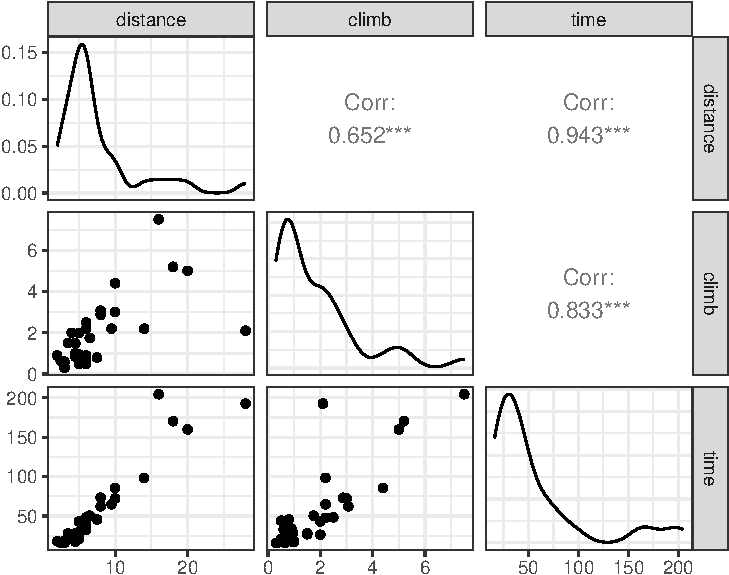
\includegraphics{r-demo-part-1_files/figure-pdf/unnamed-chunk-4-1.pdf}

}

\end{figure}

\begin{Shaded}
\begin{Highlighting}[]
\CommentTok{\# mile time versus distance}

\CommentTok{\# Q: How does mile time vary with distance?}
\CommentTok{\# Q: What races deviate from this trend?}
\CommentTok{\# Q: How does climb play into it?}

\CommentTok{\# add mile time variable to scots\_races}
\NormalTok{scots\_races }\OtherTok{\textless{}{-}}\NormalTok{ scots\_races }\SpecialCharTok{|\textgreater{}}
  \FunctionTok{mutate}\NormalTok{(}\AttributeTok{mile\_time =}\NormalTok{ time }\SpecialCharTok{/}\NormalTok{ distance) }\CommentTok{\# mutate() from dplyr to add column}
\end{Highlighting}
\end{Shaded}

\begin{Shaded}
\begin{Highlighting}[]
\CommentTok{\# plot mile time versus distance}
\NormalTok{scots\_races }\SpecialCharTok{|\textgreater{}}
  \FunctionTok{ggplot}\NormalTok{(}\FunctionTok{aes}\NormalTok{(}\AttributeTok{x =}\NormalTok{ distance, }\AttributeTok{y =}\NormalTok{ mile\_time)) }\SpecialCharTok{+}
  \FunctionTok{geom\_point}\NormalTok{()}
\end{Highlighting}
\end{Shaded}

\begin{figure}[H]

{\centering 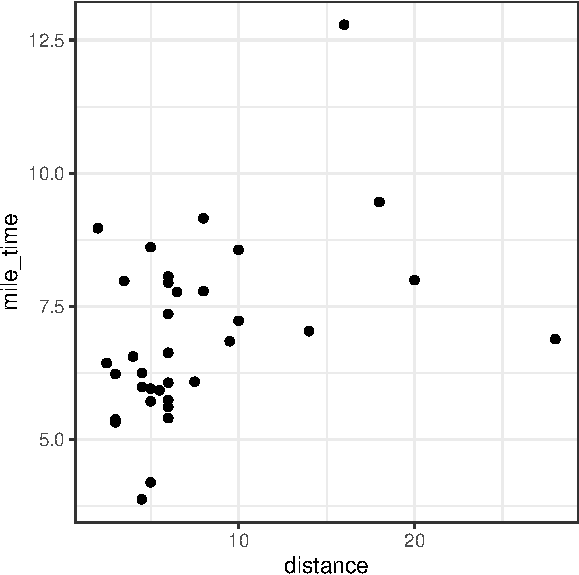
\includegraphics{r-demo-part-1_files/figure-pdf/unnamed-chunk-5-1.pdf}

}

\end{figure}

\begin{Shaded}
\begin{Highlighting}[]
\CommentTok{\# add climb information as point color}
\NormalTok{scots\_races }\SpecialCharTok{|\textgreater{}}
  \FunctionTok{ggplot}\NormalTok{(}\FunctionTok{aes}\NormalTok{(}\AttributeTok{x =}\NormalTok{ distance, }\AttributeTok{y =}\NormalTok{ mile\_time, }\AttributeTok{colour =}\NormalTok{ climb)) }\SpecialCharTok{+}
  \FunctionTok{geom\_point}\NormalTok{()}
\end{Highlighting}
\end{Shaded}

\begin{figure}[H]

{\centering 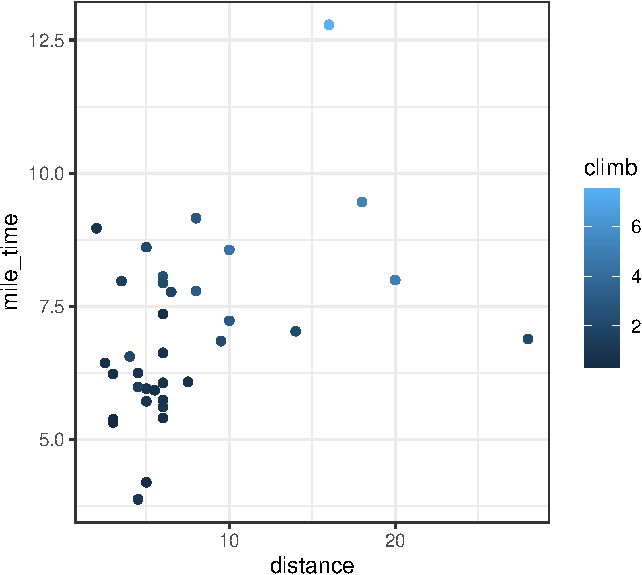
\includegraphics{r-demo-part-1_files/figure-pdf/unnamed-chunk-6-1.pdf}

}

\end{figure}

\begin{Shaded}
\begin{Highlighting}[]
\CommentTok{\# highlight extreme points}
\NormalTok{scots\_races\_extreme }\OtherTok{\textless{}{-}}\NormalTok{ scots\_races }\SpecialCharTok{|\textgreater{}}
  \FunctionTok{filter}\NormalTok{(distance }\SpecialCharTok{\textgreater{}} \DecValTok{15} \SpecialCharTok{|}\NormalTok{ mile\_time }\SpecialCharTok{\textgreater{}} \DecValTok{9}\NormalTok{) }\CommentTok{\# filter() from dplyr to subset rows}

\CommentTok{\# plot mile time versus distance}
\NormalTok{scots\_races }\SpecialCharTok{|\textgreater{}}
  \FunctionTok{ggplot}\NormalTok{(}\FunctionTok{aes}\NormalTok{(}\AttributeTok{x =}\NormalTok{ distance, }\AttributeTok{y =}\NormalTok{ mile\_time, }\AttributeTok{label =}\NormalTok{ race, }\AttributeTok{colour =}\NormalTok{ climb)) }\SpecialCharTok{+}
  \FunctionTok{geom\_point}\NormalTok{() }\SpecialCharTok{+}
  \FunctionTok{geom\_text\_repel}\NormalTok{(}\FunctionTok{aes}\NormalTok{(}\AttributeTok{label =}\NormalTok{ race), }\AttributeTok{data =}\NormalTok{ scots\_races\_extreme)}
\end{Highlighting}
\end{Shaded}

\begin{figure}[H]

{\centering 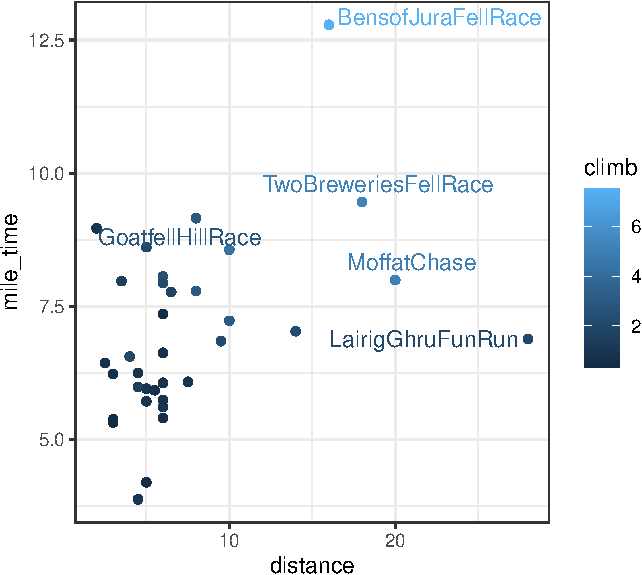
\includegraphics{r-demo-part-1_files/figure-pdf/unnamed-chunk-7-1.pdf}

}

\end{figure}

\begin{Shaded}
\begin{Highlighting}[]
\CommentTok{\# clean up plot}
\NormalTok{scots\_races }\SpecialCharTok{|\textgreater{}}
  \FunctionTok{ggplot}\NormalTok{(}\FunctionTok{aes}\NormalTok{(}\AttributeTok{x =}\NormalTok{ distance, }\AttributeTok{y =}\NormalTok{ mile\_time, }\AttributeTok{label =}\NormalTok{ race, }\AttributeTok{color =}\NormalTok{ climb)) }\SpecialCharTok{+}
  \FunctionTok{geom\_point}\NormalTok{() }\SpecialCharTok{+}
  \FunctionTok{geom\_text\_repel}\NormalTok{(}\FunctionTok{aes}\NormalTok{(}\AttributeTok{label =}\NormalTok{ race), }\AttributeTok{data =}\NormalTok{ scots\_races\_extreme) }\SpecialCharTok{+}
  \FunctionTok{labs}\NormalTok{(}
    \AttributeTok{x =} \StringTok{"Distance (miles)"}\NormalTok{,}
    \AttributeTok{y =} \StringTok{"Mile Time (minutes per mile)"}\NormalTok{,}
    \AttributeTok{color =} \StringTok{"Climb}\SpecialCharTok{\textbackslash{}n}\StringTok{(thousands of ft)"}
\NormalTok{  )}
\end{Highlighting}
\end{Shaded}

\begin{figure}[H]

{\centering 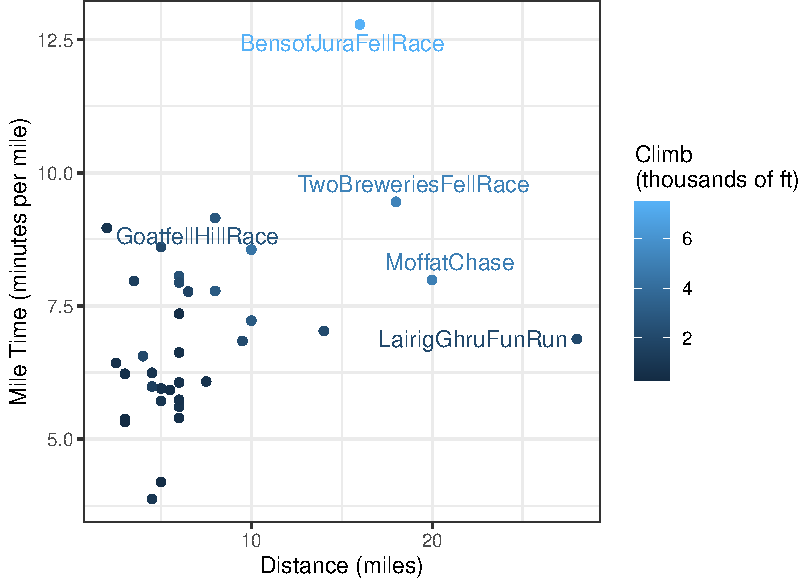
\includegraphics{r-demo-part-1_files/figure-pdf/unnamed-chunk-8-1.pdf}

}

\end{figure}

\hypertarget{linear-model-coefficient-interpretation}{%
\section{Linear model coefficient
interpretation}\label{linear-model-coefficient-interpretation}}

Let's fit some linear models and interpret the coefficients.

\begin{Shaded}
\begin{Highlighting}[]
\CommentTok{\# Q: What is the effect of an extra mile of distance on time?}

\NormalTok{lm\_fit }\OtherTok{\textless{}{-}} \FunctionTok{lm}\NormalTok{(time }\SpecialCharTok{\textasciitilde{}}\NormalTok{ distance }\SpecialCharTok{+}\NormalTok{ climb, }\AttributeTok{data =}\NormalTok{ scots\_races)}
\FunctionTok{coef}\NormalTok{(lm\_fit)}
\end{Highlighting}
\end{Shaded}

\begin{verbatim}
(Intercept)    distance       climb 
 -13.108551    6.350955   11.780133 
\end{verbatim}

\begin{Shaded}
\begin{Highlighting}[]
\CommentTok{\# Linear model with interaction}

\CommentTok{\# Q: What is the effect of an extra mile of distance on time}
\CommentTok{\#  for a run with low climb?}

\CommentTok{\# Q: What is the effect of an extra mile of distance on time}
\CommentTok{\#  for a run with high climb?}

\NormalTok{lm\_fit\_int }\OtherTok{\textless{}{-}} \FunctionTok{lm}\NormalTok{(time }\SpecialCharTok{\textasciitilde{}}\NormalTok{ distance }\SpecialCharTok{*}\NormalTok{ climb, }\AttributeTok{data =}\NormalTok{ scots\_races)}
\FunctionTok{coef}\NormalTok{(lm\_fit\_int)}
\end{Highlighting}
\end{Shaded}

\begin{verbatim}
   (Intercept)       distance          climb distance:climb 
    -0.7671925      4.9622542      3.7132519      0.6598256 
\end{verbatim}

\begin{Shaded}
\begin{Highlighting}[]
\NormalTok{scots\_races }\SpecialCharTok{|\textgreater{}}
  \FunctionTok{summarise}\NormalTok{(}\AttributeTok{min\_climb =} \FunctionTok{min}\NormalTok{(climb), }\AttributeTok{max\_climb =} \FunctionTok{max}\NormalTok{(climb))}
\end{Highlighting}
\end{Shaded}

\begin{verbatim}
# A tibble: 1 x 2
  min_climb max_climb
      <dbl>     <dbl>
1       0.3       7.5
\end{verbatim}

Let's take a look at the regression summary for \texttt{lm\_fit}:

\begin{Shaded}
\begin{Highlighting}[]
\NormalTok{lm\_fit }\OtherTok{\textless{}{-}} \FunctionTok{lm}\NormalTok{(time }\SpecialCharTok{\textasciitilde{}}\NormalTok{ distance }\SpecialCharTok{+}\NormalTok{ climb, }\AttributeTok{data =}\NormalTok{ scots\_races)}
\FunctionTok{summary}\NormalTok{(lm\_fit)}
\end{Highlighting}
\end{Shaded}

\begin{verbatim}

Call:
lm(formula = time ~ distance + climb, data = scots_races)

Residuals:
    Min      1Q  Median      3Q     Max 
-16.654  -4.842   1.110   4.667  27.762 

Coefficients:
            Estimate Std. Error t value Pr(>|t|)    
(Intercept) -13.1086     2.5608  -5.119 1.41e-05 ***
distance      6.3510     0.3578  17.751  < 2e-16 ***
climb        11.7801     1.2206   9.651 5.37e-11 ***
---
Signif. codes:  0 '***' 0.001 '**' 0.01 '*' 0.05 '.' 0.1 ' ' 1

Residual standard error: 8.734 on 32 degrees of freedom
Multiple R-squared:  0.9717,    Adjusted R-squared:   0.97 
F-statistic: 549.9 on 2 and 32 DF,  p-value: < 2.2e-16
\end{verbatim}

We get a coefficient of 6.35 with standard error 0.36 for
\texttt{distance}, where the standard error is an estimate of the
quantity (\ref{eq-conditional-variance}).

\hypertarget{r2-and-sum-of-squared-decompositions.}{%
\section{\texorpdfstring{\(R^2\) and sum-of-squared
decompositions.}{R\^{}2 and sum-of-squared decompositions.}}\label{r2-and-sum-of-squared-decompositions.}}

We can extract the \(R^2\) from this fit by reading it off from the
bottom of the summary, or by typing

\begin{Shaded}
\begin{Highlighting}[]
\FunctionTok{summary}\NormalTok{(lm\_fit)}\SpecialCharTok{$}\NormalTok{r.squared}
\end{Highlighting}
\end{Shaded}

\begin{verbatim}
[1] 0.971725
\end{verbatim}

We can construct sum-of-squares decompositions
(\ref{eq-pythagorean-theorem}) using the \texttt{anova} function. This
function takes as arguments the partial model and the full model. For
example, consider the partial model
\texttt{time\ \textasciitilde{}\ distance}.

\begin{Shaded}
\begin{Highlighting}[]
\NormalTok{lm\_fit\_partial }\OtherTok{\textless{}{-}} \FunctionTok{lm}\NormalTok{(time }\SpecialCharTok{\textasciitilde{}}\NormalTok{ distance, }\AttributeTok{data =}\NormalTok{ scots\_races)}
\FunctionTok{anova}\NormalTok{(lm\_fit\_partial, lm\_fit)}
\end{Highlighting}
\end{Shaded}

\begin{verbatim}
Analysis of Variance Table

Model 1: time ~ distance
Model 2: time ~ distance + climb
  Res.Df    RSS Df Sum of Sq     F    Pr(>F)    
1     33 9546.9                                 
2     32 2441.3  1    7105.6 93.14 5.369e-11 ***
---
Signif. codes:  0 '***' 0.001 '**' 0.01 '*' 0.05 '.' 0.1 ' ' 1
\end{verbatim}

We find that adding the predictor \texttt{climb} reduces the RSS by
7106, from 9547 to 2441. As another example, we can compute the \(R^2\)
by comparing the full model with the null model:

\begin{Shaded}
\begin{Highlighting}[]
\NormalTok{lm\_fit\_null }\OtherTok{\textless{}{-}} \FunctionTok{lm}\NormalTok{(time }\SpecialCharTok{\textasciitilde{}} \DecValTok{1}\NormalTok{, }\AttributeTok{data =}\NormalTok{ scots\_races)}
\FunctionTok{anova}\NormalTok{(lm\_fit\_null, lm\_fit)}
\end{Highlighting}
\end{Shaded}

\begin{verbatim}
Analysis of Variance Table

Model 1: time ~ 1
Model 2: time ~ distance + climb
  Res.Df   RSS Df Sum of Sq      F    Pr(>F)    
1     34 86340                                  
2     32  2441  2     83899 549.87 < 2.2e-16 ***
---
Signif. codes:  0 '***' 0.001 '**' 0.01 '*' 0.05 '.' 0.1 ' ' 1
\end{verbatim}

Therefore, the \(R^2\) is 83899/86340 = 0.972, consistent with the above
regression summary.

\hypertarget{adjustment-and-collinearity.}{%
\section{Adjustment and
collinearity.}\label{adjustment-and-collinearity.}}

We can also test the adjustment formula (\ref{eq-orthogonal-univariate})
numerically. Let's consider the coefficient of \texttt{distance} in the
regression \texttt{time\ \textasciitilde{}\ distance\ +\ climb}. We can
obtain this coefficient by first regressing \texttt{climb} out of
\texttt{distance} and \texttt{time}:

\begin{Shaded}
\begin{Highlighting}[]
\NormalTok{lm\_dist\_on\_climb }\OtherTok{\textless{}{-}} \FunctionTok{lm}\NormalTok{(distance }\SpecialCharTok{\textasciitilde{}}\NormalTok{ climb, }\AttributeTok{data =}\NormalTok{ scots\_races)}
\NormalTok{lm\_time\_on\_climb }\OtherTok{\textless{}{-}} \FunctionTok{lm}\NormalTok{(time }\SpecialCharTok{\textasciitilde{}}\NormalTok{ climb, }\AttributeTok{data =}\NormalTok{ scots\_races)}

\NormalTok{scots\_races\_resid }\OtherTok{\textless{}{-}} \FunctionTok{tibble}\NormalTok{(}
  \AttributeTok{dist\_residuals =} \FunctionTok{residuals}\NormalTok{(lm\_dist\_on\_climb),}
  \AttributeTok{time\_residuals =} \FunctionTok{residuals}\NormalTok{(lm\_time\_on\_climb)}
\NormalTok{)}

\NormalTok{lm\_adjusted }\OtherTok{\textless{}{-}} \FunctionTok{lm}\NormalTok{(time\_residuals }\SpecialCharTok{\textasciitilde{}}\NormalTok{ dist\_residuals }\SpecialCharTok{{-}} \DecValTok{1}\NormalTok{,}
  \AttributeTok{data =}\NormalTok{ scots\_races\_resid}
\NormalTok{)}
\FunctionTok{summary}\NormalTok{(lm\_adjusted)}
\end{Highlighting}
\end{Shaded}

\begin{verbatim}

Call:
lm(formula = time_residuals ~ dist_residuals - 1, data = scots_races_resid)

Residuals:
    Min      1Q  Median      3Q     Max 
-16.654  -4.842   1.110   4.667  27.762 

Coefficients:
               Estimate Std. Error t value Pr(>|t|)    
dist_residuals   6.3510     0.3471    18.3   <2e-16 ***
---
Signif. codes:  0 '***' 0.001 '**' 0.01 '*' 0.05 '.' 0.1 ' ' 1

Residual standard error: 8.474 on 34 degrees of freedom
Multiple R-squared:  0.9078,    Adjusted R-squared:  0.9051 
F-statistic: 334.8 on 1 and 34 DF,  p-value: < 2.2e-16
\end{verbatim}

We find a coefficient of 6.35 with standard error 0.35, which matches
that obtained in the original regression.

We can get the partial correlation between \texttt{distance} and
\texttt{time} by taking the empirical correlation between the residuals.
We can compare this quantity to the usual correlation.

\begin{Shaded}
\begin{Highlighting}[]
\NormalTok{scots\_races\_resid }\SpecialCharTok{|\textgreater{}}
  \FunctionTok{summarise}\NormalTok{(}\FunctionTok{cor}\NormalTok{(dist\_residuals, time\_residuals)) }\SpecialCharTok{|\textgreater{}}
  \FunctionTok{pull}\NormalTok{()}
\end{Highlighting}
\end{Shaded}

\begin{verbatim}
[1] 0.9527881
\end{verbatim}

\begin{Shaded}
\begin{Highlighting}[]
\NormalTok{scots\_races }\SpecialCharTok{|\textgreater{}}
  \FunctionTok{summarise}\NormalTok{(}\FunctionTok{cor}\NormalTok{(distance, time)) }\SpecialCharTok{|\textgreater{}}
  \FunctionTok{pull}\NormalTok{()}
\end{Highlighting}
\end{Shaded}

\begin{verbatim}
[1] 0.9430944
\end{verbatim}

In this case, the two correlation quantities are similar.

To obtain the variance inflation factors defined in equation
(\ref{eq-vif}), we can use the \texttt{vif} function from the
\texttt{car} package:

\begin{Shaded}
\begin{Highlighting}[]
\FunctionTok{vif}\NormalTok{(lm\_fit)}
\end{Highlighting}
\end{Shaded}

\begin{verbatim}
distance    climb 
1.740812 1.740812 
\end{verbatim}

Why are these two VIF values the same?

\part{Linear models: Inference}

We now understand the least squares estimator
\(\boldsymbol{\widehat{\beta}}\) from geometric and algebraic points of
view. In Unit 2, we switch to a probabilistic perspective to derive
inferential statements for linear models, in the form of hypothesis
tests and confidence intervals. In order to facilitate this, we will
assume that the error terms are normally distributed:

\[
\boldsymbol{y} = \boldsymbol{X} \boldsymbol{\beta} + \boldsymbol{\epsilon}, \quad \text{where} \ \boldsymbol{\epsilon} \sim N(\boldsymbol{0}, \sigma^2 \boldsymbol{I}_n).
\] We first establish some building blocks necessary for linear models
inference, primarily related to manipulating the normal distribution
(Chapter~\ref{sec-building-blocks}). Then, we discuss univariate and
multivariate hypothesis testing in linear models
(Chapter~\ref{sec-hypothesis-testing-chapter}), as well as the power of
these hypothesis tests (Chapter~\ref{sec-power}). We then move on to the
construction of confidence intervals and confidence regions
(Chapter~\ref{sec-confidence-intervals}). We conclude with a discussion
of practical considerations (Chapter~\ref{sec-practical-considerations})
and an R demo (Chapter~\ref{sec-r-demo-part-2}).

\hypertarget{sec-building-blocks}{%
\chapter{Building blocks}\label{sec-building-blocks}}

\emph{See also Agresti 3.1.1, 3.1.2, 3.1.4}

First we put in place some building blocks: The multivariate normal
distribution (Section~\ref{sec-mvrnorm}), the distributions of linear
regression estimates and residuals (Section~\ref{sec-lin-reg-dist}), and
estimation of the noise variance \(\sigma^2\)
(Section~\ref{sec-noise-estimation}).

\hypertarget{sec-mvrnorm}{%
\section{The multivariate normal distribution}\label{sec-mvrnorm}}

Recall that a random vector \(\boldsymbol{w} \in \mathbb{R}^d\) has a
multivariate normal distribution with mean \(\boldsymbol{\mu}\) and
covariance matrix \(\boldsymbol{\Sigma}\) if it has probability density

\[
p(\boldsymbol{w}) = \frac{1}{\sqrt{(2\pi)^{d}\text{det}(\boldsymbol{\Sigma})}}\exp\left(-\frac{1}{2}(\boldsymbol{w} - \boldsymbol{\mu})^\top \boldsymbol{\Sigma}^{-1}(\boldsymbol{w} - \boldsymbol{\mu})\right).
\]

It is also possible to define normal distributions in the case
\(\text{det}(\boldsymbol\Sigma) = 0\). These distributions are supported
on subspaces of \(\mathbb{R}^d\), and do not have densities with respect
to the Lebesgue measure.

These random vectors have lots of special properties, including:

\begin{itemize}
\tightlist
\item
  \textbf{Linear transformation}: If
  \(\boldsymbol{w} \sim N(\boldsymbol{\mu}, \boldsymbol{\Sigma})\), then
  \(\boldsymbol{A} \boldsymbol{w} + \boldsymbol{b} \sim N(\boldsymbol{A} \boldsymbol{\mu} + \boldsymbol{b}, \boldsymbol{A} \boldsymbol{\Sigma} \boldsymbol{A}^\top)\).
\item
  \textbf{Independence}: If \[
  \begin{pmatrix}\boldsymbol{w}_1 \\ \boldsymbol{w}_2 \end{pmatrix} \sim N\left(\begin{pmatrix}\boldsymbol{\mu}_1 \\ \boldsymbol{\mu}_2 \end{pmatrix} , \begin{pmatrix}\boldsymbol{\Sigma}_{11} & \boldsymbol{\Sigma}_{12} \\ \boldsymbol{\Sigma}_{12}^\top & \boldsymbol{\Sigma}_{22}\end{pmatrix}\right),
  \] then \(\boldsymbol{w}_1 \perp\!\!\!\perp \boldsymbol{w}_2\) if and
  only if \(\boldsymbol{\Sigma}_{12} = \boldsymbol{0}\).
\end{itemize}

An important distribution related to the multivariate normal is the
\(\chi^2_d\) (chi-squared with \(d\) degrees of freedom) distribution,
defined as

\[
\chi^2_d \equiv \sum_{j = 1}^d w_j^2 \quad \text{for} \quad w_1, \dots, w_d \overset{\text{i.i.d.}}{\sim} N(0, 1).
\]

\hypertarget{sec-lin-reg-dist}{%
\section{The distributions of linear regression estimates and
residuals}\label{sec-lin-reg-dist}}

\emph{See also Dunn and Smyth 2.8.2}

The most important distributional result in linear regression is that

\begin{equation}\protect\hypertarget{eq-beta-hat-dist}{}{
\boldsymbol{\widehat{\beta}} \sim N(\boldsymbol{\beta}, \sigma^2 (\boldsymbol{X}^\top \boldsymbol{X})^{-1}).
}\label{eq-beta-hat-dist}\end{equation}

Indeed, by the linear transformation property of the multivariate normal
distribution,\(\boldsymbol{y} \sim N(\boldsymbol{X} \boldsymbol{\beta}, \sigma^2 \boldsymbol{I}_n)\)
implies that

\[
\begin{split}
\boldsymbol{\widehat{\beta}} &= (\boldsymbol{X}^\top \boldsymbol{X})^{-1}\boldsymbol{X}^\top \boldsymbol{y} \\
&\sim N((\boldsymbol{X}^\top \boldsymbol{X})^{-1}\boldsymbol{X}^\top \boldsymbol{X} \boldsymbol{\beta}, (\boldsymbol{X}^\top \boldsymbol{X})^{-1}\boldsymbol{X}^\top \sigma^2 \boldsymbol{I}_n \boldsymbol{X}(\boldsymbol{X}^\top \boldsymbol{X})^{-1}) \\
&= N(\boldsymbol{\beta}, \sigma^2 (\boldsymbol{X}^\top \boldsymbol{X})^{-1}).
\end{split}
\]

Next, let's consider the joint distribution of
\(\boldsymbol{\widehat{\mu}} = \boldsymbol{X} \boldsymbol{\widehat{\beta}}\)
and
\(\boldsymbol{\widehat{\epsilon}} = \boldsymbol{y} - \boldsymbol{X} \boldsymbol{\widehat{\beta}}\).
We have

\[
\begin{split}
\begin{pmatrix} \boldsymbol{\widehat{\mu}} \\ \boldsymbol{\widehat{\epsilon}} \end{pmatrix} &= \begin{pmatrix} \boldsymbol{H} \boldsymbol{y} \\ (\boldsymbol{I} - \boldsymbol{H}) \boldsymbol{y} \end{pmatrix} \\
&= \begin{pmatrix} \boldsymbol{H} \\ \boldsymbol{I} - \boldsymbol{H} \end{pmatrix}\boldsymbol{y} \\
&\sim N\left(\begin{pmatrix} \boldsymbol{H} \\ \boldsymbol{I} - \boldsymbol{H} \end{pmatrix}\boldsymbol{X} \boldsymbol{\beta}, \begin{pmatrix} \boldsymbol{H} \\ \boldsymbol{I} - \boldsymbol{H} \end{pmatrix}\cdot \sigma^2 \boldsymbol{I} \begin{pmatrix} \boldsymbol{H} & \boldsymbol{I} - \boldsymbol{H} \end{pmatrix}\right)
\\
&= N\left(\begin{pmatrix} \boldsymbol{X} \boldsymbol{\beta} \\ \boldsymbol{0} \end{pmatrix}, \begin{pmatrix} \sigma^2 \boldsymbol{H} & \boldsymbol{0} \\ \boldsymbol{0} & \sigma^2(\boldsymbol{I} - \boldsymbol{H}) \end{pmatrix} \right).
\end{split}
\]

In other words,

\begin{equation}\protect\hypertarget{eq-fit-and-error-dist}{}{
\boldsymbol{\widehat{\mu}} \sim N(\boldsymbol{X} \boldsymbol{\beta}, \sigma^2 \boldsymbol{H}) \quad \text{and} \quad \boldsymbol{\widehat{\epsilon}} \sim N(\boldsymbol{0}, \sigma^2(\boldsymbol{I} - \boldsymbol{H})), \quad \text{with} \quad \boldsymbol{\widehat{\mu}} \perp\!\!\!\perp \boldsymbol{\widehat{\epsilon}}.
}\label{eq-fit-and-error-dist}\end{equation}

The statistical independence between \(\boldsymbol{\widehat{\mu}}\) and
\(\boldsymbol{\widehat{\epsilon}}\) is a result of the fact that these
two quantities are projections of \(\boldsymbol{y}\) onto two orthogonal
subspaces: \(C(\boldsymbol{X})\) and \(C(\boldsymbol{X})^\perp\)
(Figure~\ref{fig-orthogonality-fit-residuals}).

\begin{figure}

{\centering 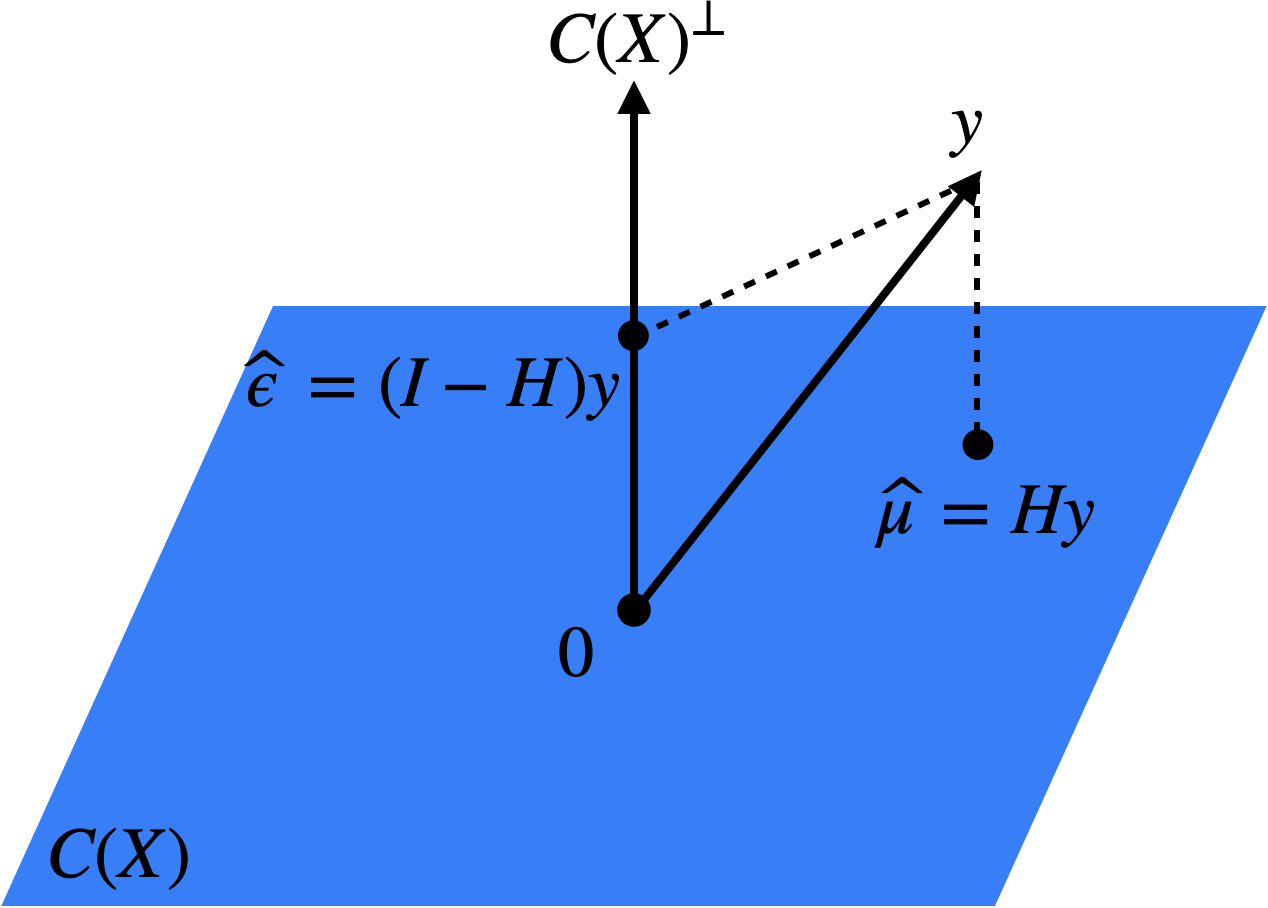
\includegraphics[width=0.5\textwidth,height=\textheight]{figures/orthogonality-fit-residuals.jpg}

}

\caption{\label{fig-orthogonality-fit-residuals}The fitted vector
\(\boldsymbol{\widehat{\mu}}\) and the residual vector
\(\boldsymbol{\widehat{\epsilon}}\) are projections of
\(\boldsymbol{y}\) onto orthogonal subspaces.}

\end{figure}

Since \(\boldsymbol{\widehat{\beta}}\) is a deterministic function of
\(\boldsymbol{\widehat{\mu}}\) (in particular,
\(\boldsymbol{\widehat{\beta}} = (\boldsymbol{X}^\top \boldsymbol{X})^{-1}\boldsymbol{X}^\top \boldsymbol{\widehat{\mu}}\)),
it also follows that

\begin{equation}\protect\hypertarget{eq-beta-ind-eps}{}{
\boldsymbol{\widehat{\beta}} \perp\!\!\!\perp \boldsymbol{\widehat{\epsilon}}.
}\label{eq-beta-ind-eps}\end{equation}

\hypertarget{sec-noise-estimation}{%
\section{\texorpdfstring{Estimation of the noise variance
\(\sigma^2\)}{Estimation of the noise variance \textbackslash sigma\^{}2}}\label{sec-noise-estimation}}

\emph{See also Dunn and Smyth 2.4.2, 2.5.3}

We can't quite do inference for \(\boldsymbol{\beta}\) based on the
distributional result (\ref{eq-beta-hat-dist}) because the noise
variance \(\sigma^2\) is unknown to us. Intuitively, since
\(\sigma^2 = \mathbb{E}[\epsilon_i^2]\), we can get an estimate of
\(\sigma^2\) by looking at the quantity
\(\|\boldsymbol{\widehat{\epsilon}}\|^2\). To get the distribution of
this quantity, we need the following lemma:

\begin{lemma}[]\protect\hypertarget{lem-normal-projection}{}\label{lem-normal-projection}

Let \(\boldsymbol{w} \sim N(\boldsymbol{0}, \boldsymbol{P})\) for some
projection matrix \(\boldsymbol{P}\). Then,
\(\|\boldsymbol{w}\|^2 \sim \chi^2_d\), where
\(d = \text{trace}(\boldsymbol{P})\) is the dimension of the subspace
onto which \(\boldsymbol{P}\) projects.

\end{lemma}

\begin{proof}

Let
\(\boldsymbol{P} = \boldsymbol{U} \boldsymbol{D} \boldsymbol{U}^\top\)
be an eigenvalue decomposition of \(\boldsymbol{P}\), where
\(\boldsymbol{U}\) is orthogonal and \(\boldsymbol{D}\) is a diagonal
matrix with \(D_{ii} \in \{0,1\}\). We have
\(\boldsymbol{w} \overset{d}{=} \boldsymbol{U} \boldsymbol{D} \boldsymbol{z}\)
for \(\boldsymbol{z} \sim N(0, \boldsymbol{I}_n)\). Therefore,

\[
\|\boldsymbol{w}\|^2 = \|\boldsymbol{D} \boldsymbol{z}\|^2 = \sum_{i: D_{ii} = 1} z_i^2 \sim \chi^2_d, \quad \text{where } d = |\{i: D_{ii} = 1\}| = \text{trace}(D) = \text{trace}(\boldsymbol{P}).
\]

\end{proof}

Recall that \(\boldsymbol{I} - \boldsymbol{H}\) is a projection onto the
\((n-p)\)-dimensional space \(C(\boldsymbol{X})^\perp\), so by
Lemma~\ref{lem-normal-projection} and equation
(\ref{eq-fit-and-error-dist}), we have

\begin{equation}\protect\hypertarget{eq-eps-norm-dist}{}{
\|\boldsymbol{\widehat{\epsilon}}\|^2 \sim \sigma^2 \chi^2_{n-p}.
}\label{eq-eps-norm-dist}\end{equation}

From this result, it follows that
\(\mathbb{E}[\|\boldsymbol{\widehat{\epsilon}}\|^2] = \sigma^2(n-p)\),
so

\begin{equation}\protect\hypertarget{eq-unbiased-noise-estimate}{}{
\widehat{\sigma}^2 \equiv \frac{1}{n-p}\|\boldsymbol{\widehat{\epsilon}}\|^2
}\label{eq-unbiased-noise-estimate}\end{equation}

is an unbiased estimate for \(\sigma^2\). Why does the denominator need
to be \(n-p\) rather than \(n\) for the estimator above to be unbiased?
The reason for this is that the residuals
\(\boldsymbol{\widehat{\epsilon}}\) are the projection of the true noise
vector \(\boldsymbol{\epsilon} \in \mathbb{R}^n\) onto the
\((n-p)\)-dimensional subspace \(C(\boldsymbol{X})^\perp\)
(Figure~\ref{fig-residuals-as-noise-projection}). To see this, note that

\[
\boldsymbol{\widehat{\epsilon}} = (\boldsymbol{I} - \boldsymbol{H})\boldsymbol{y} = (\boldsymbol{I} - \boldsymbol{H})(\boldsymbol{X} \boldsymbol{\beta} + \boldsymbol{\epsilon}) = (\boldsymbol{I} - \boldsymbol{H})\boldsymbol{\epsilon}.
\]

Therefore, the norm of the residual vector will be smaller than that of
the noise vector, especially to the extent that \(p\) is close to \(n\).

\begin{figure}

{\centering 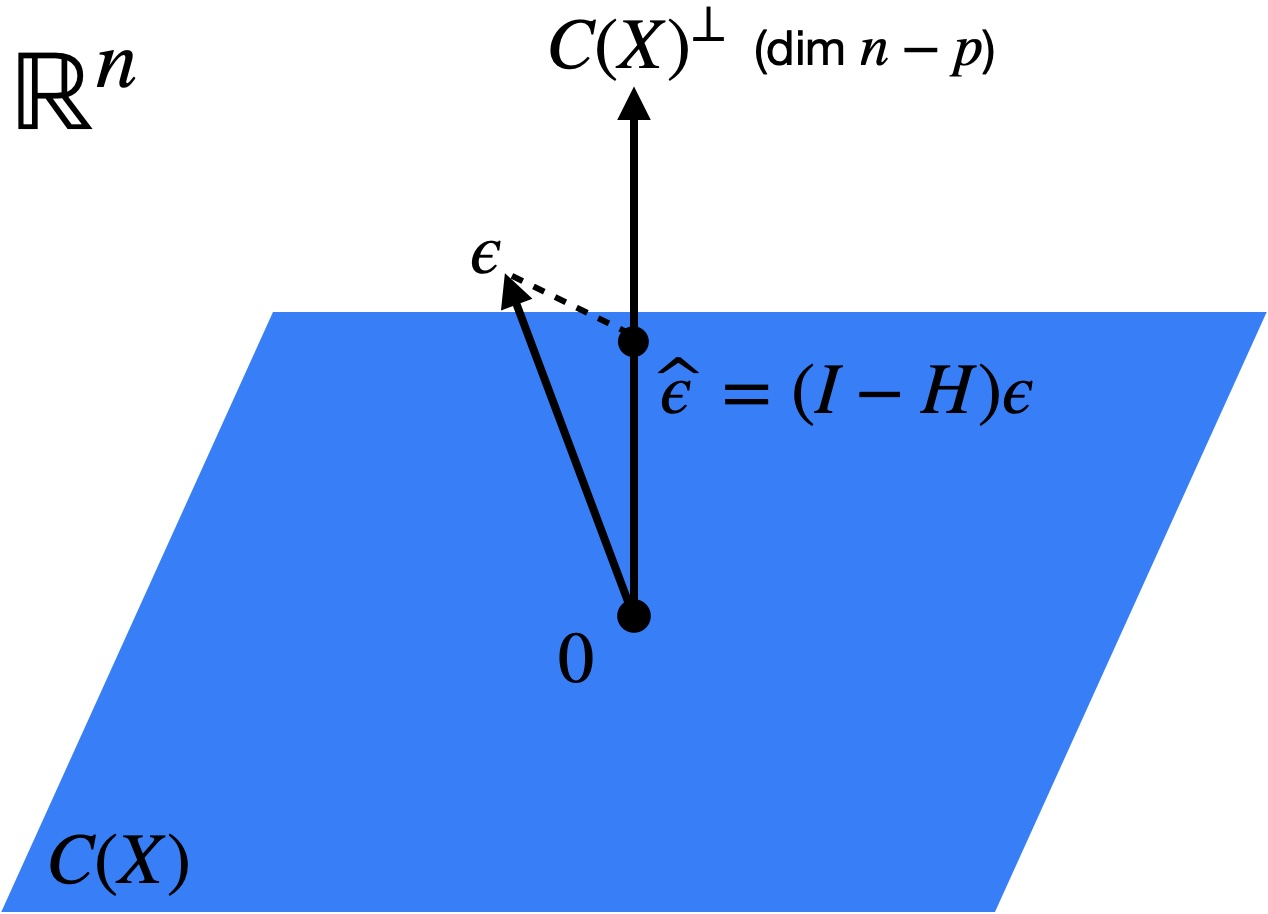
\includegraphics[width=0.5\textwidth,height=\textheight]{figures/residuals-as-noise-projection.jpg}

}

\caption{\label{fig-residuals-as-noise-projection}The residual vector
\(\boldsymbol{\widehat{\epsilon}}\) is the projection of the noise
vector \(\boldsymbol{\epsilon}\) onto \(C(\boldsymbol{X})^\perp\).}

\end{figure}

\hypertarget{sec-hypothesis-testing-chapter}{%
\chapter{Hypothesis testing}\label{sec-hypothesis-testing-chapter}}

\emph{See also Agresti 3.2.1, 3.2.2, 3.2.4, 3.2.8}

Typically, two types of null hypotheses are tested in a regression
setting: those involving one-dimensional parameters and those involving
multi-dimensional parameters. For example, consider the null hypotheses
\(H_0: \beta_j = 0\) and \(H_0: \boldsymbol{\beta}_S = \boldsymbol{0}\)
for \(S \subseteq \{0, 1, \dots, p-1\}\), respectively. We discuss tests
of these two kinds of hypotheses in Sections \ref{sec-one-dim-testing}
and \ref{sec-multi-dim-testing}, and then discuss the power of these
tests in Chapter~\ref{sec-power}.

\hypertarget{sec-one-dim-testing}{%
\section{Testing a one-dimensional
parameter}\label{sec-one-dim-testing}}

\emph{See also Dunn and Smyth 2.8.3}

\hypertarget{t-test-for-a-single-coefficient}{%
\subsection{\texorpdfstring{\(t\)-test for a single
coefficient}{t-test for a single coefficient}}\label{t-test-for-a-single-coefficient}}

The most common question to ask in a linear regression context is: Is
the \(j\)th predictor associated with the response when controlling for
the other predictors? In the language of hypothesis testing, this
corresponds to the null hypothesis:

\begin{equation}\protect\hypertarget{eq-one-dim-null}{}{
H_0: \beta_j = 0
}\label{eq-one-dim-null}\end{equation}

According to equation (\ref{eq-beta-hat-dist}), we have
\(\widehat{\beta}_j \sim N(0, \sigma^2/s_j^2)\), where, as we learned in
Chapter 1:

\[
s_j^{2} \equiv [(\boldsymbol{X}^T \boldsymbol{X})^{-1}_{jj}]^{-1} = \|\boldsymbol{x}_{*j}^\perp\|^2.
\]

Therefore,

\begin{equation}\protect\hypertarget{eq-oracle-z-stat}{}{
\frac{\widehat{\beta}_j}{\sigma/s_j} \sim N(0,1),
}\label{eq-oracle-z-stat}\end{equation}

and we are tempted to define a level \(\alpha\) test of the null
hypothesis (\ref{eq-one-dim-null}) based on this normal distribution.
While this is infeasible since we don't know \(\sigma^2\), we can
substitute in the unbiased estimate (\ref{eq-unbiased-noise-estimate})
derived in Section~\ref{sec-noise-estimation}. Then,

\[
\text{SE}(\widehat{\beta}_j) \equiv \frac{\widehat{\sigma}}{s_j}
\]

is the standard error of \(\widehat{\beta}_j\), which is an
approximation to the standard deviation of \(\widehat{\beta}_j\).
Dividing \(\widehat{\beta}_j\) by its standard error gives us the
\(t\)-statistic:

\[
t_j \equiv \frac{\widehat{\beta}_j}{\text{SE}(\widehat{\beta}_j)} = \frac{\widehat{\beta}_j}{\sqrt{\frac{1}{n-p}\|\boldsymbol{\widehat{\epsilon}}\|^2}/s_j}.
\]

This statistic is \emph{pivotal}, in the sense that it has the same
distribution for any \(\boldsymbol{\beta}\) such that \(\beta_j = 0\).
Indeed, we can rewrite it as:

\[
t_j = \frac{\frac{\widehat{\beta}_j}{\sigma/s_j}}{\sqrt{\frac{\sigma^{-2}\|\boldsymbol{\widehat{\epsilon}}\|^2}{n-p}}}.
\]

Recalling the independence of \(\boldsymbol{\widehat{\beta}}\) and
\(\boldsymbol{\widehat{\epsilon}}\) (\ref{eq-beta-ind-eps}), the scaled
chi-square distribution of \(\|\boldsymbol{\widehat{\epsilon}}\|^2\)
(\ref{eq-eps-norm-dist}), and the standard normal distribution of
\(\frac{\widehat{\beta}_j}{\sigma/s_j}\) (\ref{eq-oracle-z-stat}), we
find that, under \(H_0:\beta_j = 0\), \[
t_j \sim \frac{N(0,1)}{\sqrt{\frac{1}{n-p}\chi^2_{n-p}}}, \quad \text{with numerator and denominator independent.}
\]

This distribution is called the \(t\) distribution with \(n-p\) degrees
of freedom and is denoted \(t_{n-p}\). This paves the way for the
two-sided \(t\)-test:

\[
\phi_t(\boldsymbol{X}, \boldsymbol{y}) = 1(|t_j| > t_{n-p}(1-\alpha/2)),
\]

where \(t_{n-p}(1-\alpha/2)\) denotes the \(1-\alpha/2\) quantile of
\(t_{n-p}\). Note that, by the law of large numbers,

\[
\frac{1}{n-p}\chi^2_{n-p} \overset{P}{\rightarrow} 1 \quad \text{as} \quad n - p \rightarrow \infty,
\]

so for large \(n-p\) we have \(t_{j} \sim t_{n-p} \approx N(0,1)\).
Hence, the \(t\)-test is approximately equal to the following
\(z\)-test:

\[
\phi_t(\boldsymbol{X}, \boldsymbol{y}) \approx \phi_z(\boldsymbol{X}, \boldsymbol{y}) \equiv 1(|t_j| > z(1-\alpha/2)),
\]

where \(z(1-\alpha/2)\) is the \(1-\alpha/2\) quantile of \(N(0,1)\).
The \(t\)-test can also be defined in a one-sided fashion if power
against one-sided alternatives is desired.

\hypertarget{example-one-sample-model}{%
\subsection{Example: One-sample model}\label{example-one-sample-model}}

Consider the intercept-only linear regression model
\(y = \beta_0 + \epsilon\), and let usapply the \(t\)-test derived above
to test the null hypothesis \(H_0: \beta_0 = 0\). We have
\(\widehat{\beta}_0 = \bar{y}\). Furthermore, we have

\[
\text{SE}^2(\widehat{\beta}_0) = \frac{\widehat{\sigma}^2}{n}, \quad \text{where} \quad \widehat{\sigma}^2 = \frac{1}{n-1}\|\boldsymbol{y} - \bar{y} \boldsymbol{1}_n\|^2.
\]

Hence, we obtain the \(t\) statistic:

\[
t = \frac{\widehat{\beta}_0}{\text{SE}(\widehat{\beta}_0)} = \frac{\sqrt{n} \bar{y}}{\sqrt{\frac{1}{n-1}\|\boldsymbol{y} - \bar{y} \boldsymbol{1}_n\|^2}}.
\]

According to the theory above, this test statistic has a null
distribution of \(t_{n-1}\).

\hypertarget{example-two-sample-model}{%
\subsection{Example: Two-sample model}\label{example-two-sample-model}}

Suppose we have \(x_1 \in \{0,1\}\), in which case the linear regression
\(y = \beta_0 + \beta_1 x_1 + \epsilon\) becomes a two-sample model. We
can rewrite this model as:

\[
y_i \sim \begin{cases}
N(\beta_0, \sigma^2) \quad &\text{for } x_i = 0; \\
N(\beta_0 + \beta_1, \sigma^2) \quad &\text{for } x_i = 1.
\end{cases}
\]

It is often of interest to test the null hypothesis
\(H_0: \beta_1 = 0\), i.e., that the two groups have equal means. Let
usdefine:

\[
\bar{y}_0 \equiv \frac{1}{n_0}\sum_{i: x_i = 0} y_i, \quad \bar{y}_1 \equiv \frac{1}{n_1}\sum_{i: x_i = 1} y_i, \quad \text{where} \quad n_0 = |\{i: x_i = 0\}| \text{ and } n_1 = |\{i: x_i = 1\}|.
\]

Then, we have seen before that \(\widehat{\beta}_0 = \bar{y}_0\) and
\(\widehat{\beta}_1 = \bar{y}_1 - \bar{y}_0\). We can compute that:

\[
s_1^2 \equiv \|\boldsymbol{x}_{*1}^{\perp}\|^2 = \|\boldsymbol{x}_{*1} - \frac{n_1}{n}\boldsymbol{1}\|^2 = n_1\frac{n_0^2}{n^2} + n_0\frac{n_1^2}{n^2} = \frac{n_0 n_1}{n} = \frac{1}{\frac{1}{n_0} + \frac{1}{n_1}}
\]

and

\[
\widehat{\sigma}^2 = \frac{1}{n-2}\left(\sum_{i: x_i = 0}(y_i - \bar{y}_0)^2 + \sum_{i: x_i = 1}(y_i - \bar{y}_1)^2\right).
\]

Therefore, we arrive at a \(t\)-statistic of:

\[
t = \frac{\sqrt{\frac{1}{\frac{1}{n_0} + \frac{1}{n_1}}}(\bar{y}_1 - \bar{y}_0)}{\sqrt{\frac{1}{n-2}\left(\sum_{i: x_i = 0}(y_i - \bar{y}_0)^2 + \sum_{i: x_i = 1}(y_i - \bar{y}_1)^2\right)}}.
\]

Under the null hypothesis, this statistic has a distribution of
\(t_{n-2}\).

\hypertarget{t-test-for-a-contrast-among-coefficients}{%
\subsection{\texorpdfstring{\(t\)-test for a contrast among
coefficients}{t-test for a contrast among coefficients}}\label{t-test-for-a-contrast-among-coefficients}}

Given a vector \(\boldsymbol{c} \in \mathbb{R}^p\), the quantity
\(\boldsymbol{c}^T \boldsymbol{\beta}\) is sometimes called a
\emph{contrast}. For example, suppose
\(\boldsymbol{c} = (1,-1, 0, \dots, 0)\). Then,
\(\boldsymbol{c}^T \boldsymbol{\beta} = \beta_1 - \beta_2\) is the
difference in effects of the first and second predictors. We are
sometimes interested in testing whether such a contrast is equal to
zero, i.e., \(H_0: \boldsymbol{c}^T \boldsymbol{\beta} = 0\). While this
hypothesis can involve two or more of the predictors, the parameter
\(\boldsymbol{c}^T \boldsymbol{\beta}\) is still one-dimensional, and
therefore we can still apply a \(t\)-test. Going back to the
distribution
\(\boldsymbol{\widehat{\beta}} \sim N(\boldsymbol{\beta}, \sigma^2(\boldsymbol{X}^T \boldsymbol{X})^{-1})\),
we find that:

\begin{equation}\protect\hypertarget{eq-contrasts-normal-dist}{}{
\boldsymbol{c}^T\boldsymbol{\widehat{\beta}} \sim N(\boldsymbol{c}^T\boldsymbol{\beta}, \sigma^2\boldsymbol{c}^T (\boldsymbol{X}^T \boldsymbol{X})^{-1} \boldsymbol{c}).
}\label{eq-contrasts-normal-dist}\end{equation}

Therefore, under the null hypothesis that
\(\boldsymbol{c}^T \boldsymbol{\beta} = 0\), we can derive that:

\begin{equation}\protect\hypertarget{eq-contrasts-t-dist}{}{
\frac{\boldsymbol{c}^T \boldsymbol{\widehat{\beta}}}{\widehat{\sigma} \sqrt{\boldsymbol{c}^T (\boldsymbol{X}^T \boldsymbol{X})^{-1} \boldsymbol{c}}} \sim t_{n-p},
}\label{eq-contrasts-t-dist}\end{equation}

giving us another \(t\)-test. Note that the \(t\)-tests described above
can be recovered from this more general formulation by setting
\(\boldsymbol{c} = \boldsymbol{e}_j\), the indicator vector with the
\(j\)th coordinate equal to 1 and all others equal to zero.

\hypertarget{sec-multi-dim-testing}{%
\section{Testing a multi-dimensional
parameter}\label{sec-multi-dim-testing}}

\emph{See also Dunn and Smyth 2.10.1}

\hypertarget{f-test-for-a-group-of-coefficients}{%
\subsection{\texorpdfstring{\(F\)-test for a group of
coefficients}{F-test for a group of coefficients}}\label{f-test-for-a-group-of-coefficients}}

Now we move on to the case of testing a multi-dimensional parameter:
\(H_0: \boldsymbol{\beta}_S = \boldsymbol{0}\) for some
\(S \subseteq \{0, 1, \dots, p-1\}\). In other words, we would like to
test

\[
H_0: \boldsymbol{y} = \boldsymbol{X}_{*, \text{-}S} \boldsymbol{\beta}_{\text{-}S} + \boldsymbol{\epsilon} \quad \text{versus} \quad H_1: \boldsymbol{X} \boldsymbol{\beta} + \boldsymbol{\epsilon}.
\]

To test this hypothesis, let us fit least squares coefficients
\(\boldsymbol{\widehat{\beta}}_{\text{-}S}\) and
\(\boldsymbol{\widehat{\beta}}\) for the partial model as well as the
full model. If the partial model fits well, then the residuals
\(\boldsymbol{y} - \boldsymbol{X}_{*, \text{-}S} \boldsymbol{\widehat{\beta}}_{\text{-}S}\)
from this model will not be much larger than the residuals
\(\boldsymbol{y} - \boldsymbol{X} \boldsymbol{\widehat{\beta}}\) from
the full model. To quantify this intuition, let us recall our analysis
of variance decomposition from Chapter 1:

\[
\|\boldsymbol{y} - \boldsymbol{X}_{*, \text{-}S} \boldsymbol{\widehat{\beta}}_{\text{-}S}\|^2 = \|\boldsymbol{X} \boldsymbol{\widehat{\beta}} - \boldsymbol{X}_{*, \text{-}S} \boldsymbol{\widehat{\beta}}_{\text{-}S}\|^2 + \|\boldsymbol{y} - \boldsymbol{X} \boldsymbol{\widehat{\beta}}\|^2.
\]

Let us consider the ratio

\begin{equation}\protect\hypertarget{eq-f-test-ratio}{}{
\frac{\|\boldsymbol{y} - \boldsymbol{X}_{*, \text{-}S} \boldsymbol{\widehat{\beta}}_{\text{-}S}\|^2 - \|\boldsymbol{y} - \boldsymbol{X} \boldsymbol{\widehat{\beta}}\|^2}{\|\boldsymbol{y} - \boldsymbol{X} \boldsymbol{\widehat{\beta}}\|^2} = \frac{\|\boldsymbol{X} \boldsymbol{\widehat{\beta}} - \boldsymbol{X}_{*, \text{-}S} \boldsymbol{\widehat{\beta}}_{\text{-}S}\|^2}{\|\boldsymbol{y} - \boldsymbol{X} \boldsymbol{\widehat{\beta}}\|^2},
}\label{eq-f-test-ratio}\end{equation}

which is the relative increase in the residual sum of squares when going
from the full model to the partial model. To interpret this ratio
geometrically, let us first examine the quantity
\(\boldsymbol{X} \boldsymbol{\widehat{\beta}} - \boldsymbol{X}_{*, \text{-}S} \boldsymbol{\widehat{\beta}}_{\text{-}S}\)
from the numerator. Letting \(\boldsymbol{H}\) and
\(\boldsymbol{H}_{\text{-}S}\) be the projection matrices for the full
and partial models, we have \[
\boldsymbol{X} \boldsymbol{\widehat{\beta}} - \boldsymbol{X}_{*, \text{-}S} \boldsymbol{\widehat{\beta}}_{\text{-}S} = (\boldsymbol H - \boldsymbol H_{\text{-}S}) \boldsymbol{y}.
\] It turns out the the matrix
\(\boldsymbol{H} - \boldsymbol{H}_{\text{-}S}\) is a projection matrix:

\begin{proposition}[]\protect\hypertarget{prp-f-test-geometry}{}\label{prp-f-test-geometry}

The matrix \(\boldsymbol{H} - \boldsymbol{H}_{\text{-}S}\) is a
projection matrix onto the space \(C(\boldsymbol{X}_{*S}^\perp)\)
spanned by the columns of \(\boldsymbol X_{*S}\) adjusted for
\(\boldsymbol X_{*,\text{-}S}\).

\end{proposition}

Figure~\ref{fig-f-test-geometry} illustrates this relationship.

\begin{figure}

{\centering 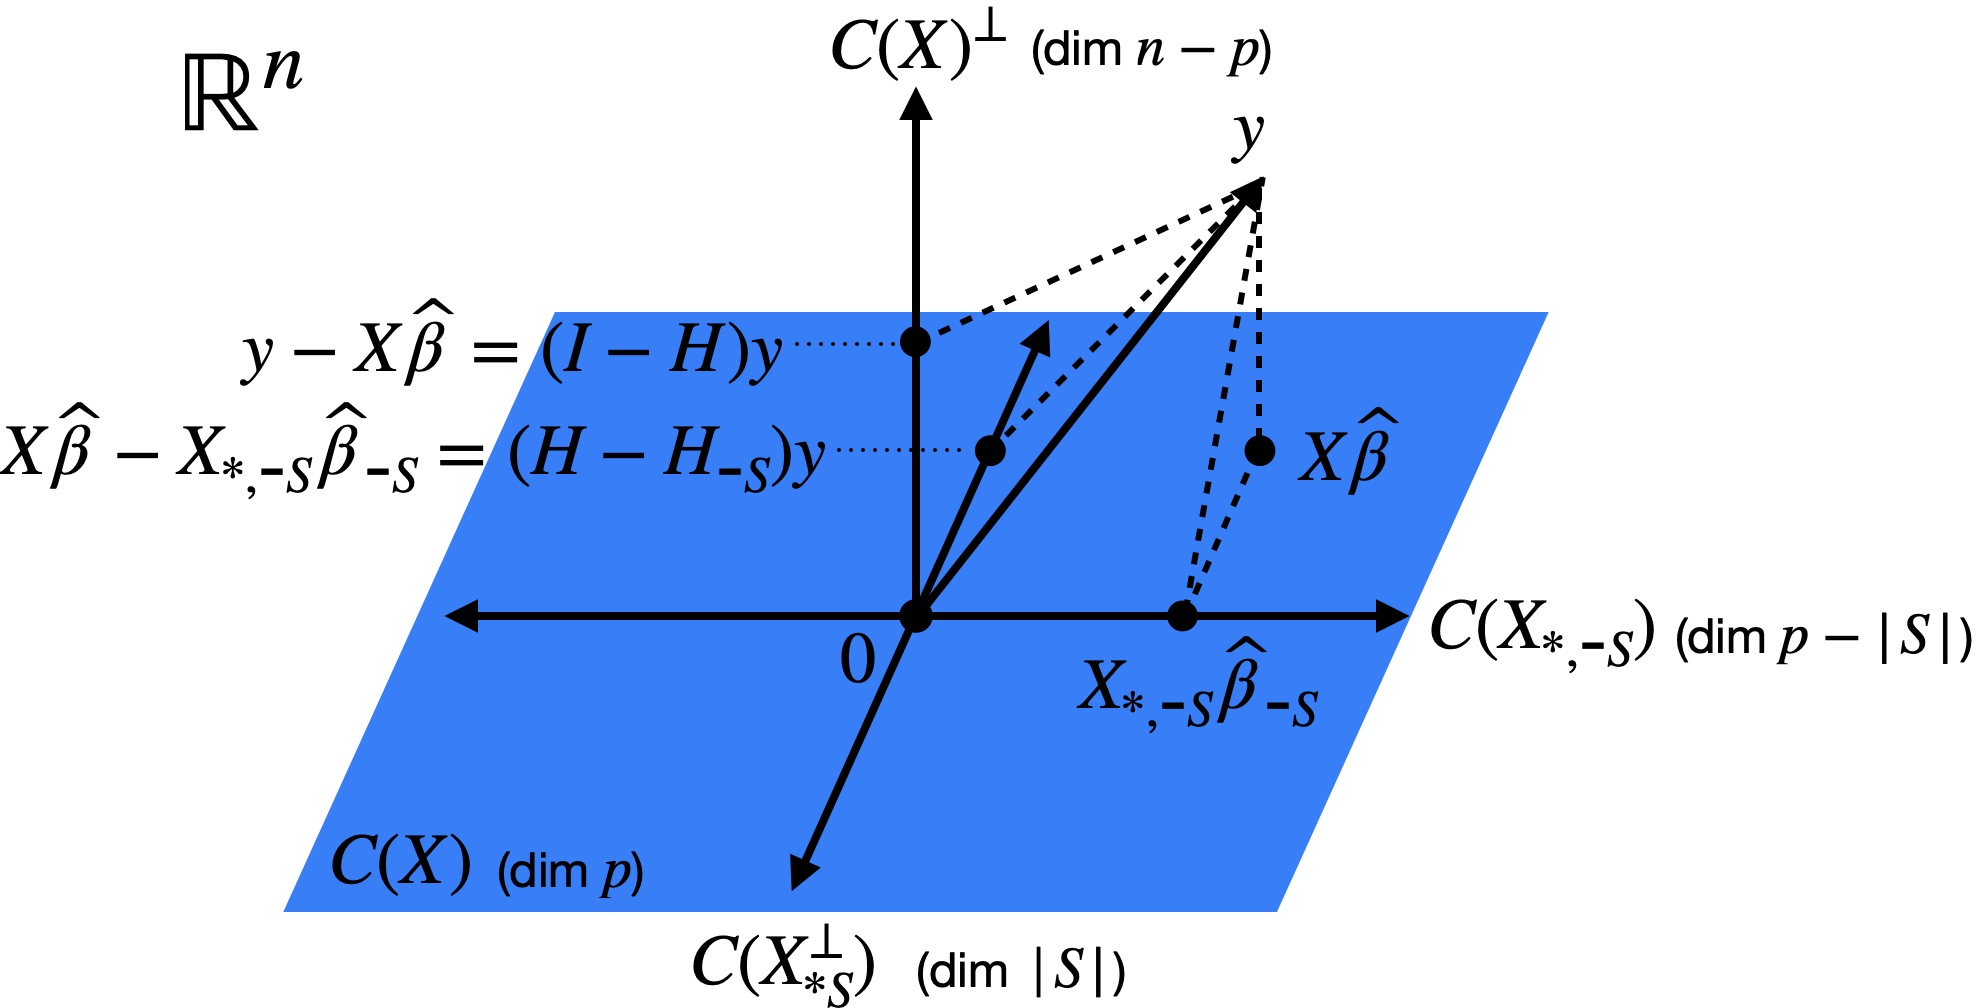
\includegraphics[width=0.75\textwidth,height=\textheight]{figures/F-test-geometry.jpg}

}

\caption{\label{fig-f-test-geometry}Geometry of the \(F\)-test.
Orthogonality relationships stem from
\(C(\boldsymbol{X}_{*,\text{-}S}) \perp C(\boldsymbol{X}_{*S}^\perp) \perp C(\boldsymbol{X})^\perp\).}

\end{figure}

\begin{proof}

Let \(\boldsymbol v \in C(\boldsymbol{X}_{*S}^\perp)\). Because
\(\boldsymbol v\) is orthogonal to \(C(\boldsymbol X_{*,\text{-}S})\) by
construction, we have
\((\boldsymbol{H} - \boldsymbol{H}_{\text{-}S})\boldsymbol v = \boldsymbol{H}\boldsymbol v - \boldsymbol{H}_{\text{-}S}\boldsymbol v = \boldsymbol v - \boldsymbol 0 = \boldsymbol v\).
On the other hand, let \(v \in C(\boldsymbol X_{*, \text{-}S})\). Then,
we have
\((\boldsymbol{H} - \boldsymbol{H}_{\text{-}S})\boldsymbol v = \boldsymbol{H}\boldsymbol v - \boldsymbol{H}_{\text{-}S}\boldsymbol v = \boldsymbol v - \boldsymbol v = \boldsymbol 0\).
Finally, let \(v \in C(\boldsymbol X)^\perp\). Then, we have
\((\boldsymbol{H} - \boldsymbol{H}_{\text{-}S})\boldsymbol v = \boldsymbol{H}\boldsymbol v - \boldsymbol{H}_{\text{-}S}\boldsymbol v = \boldsymbol 0 - \boldsymbol 0 = \boldsymbol 0\).
From these three observations, it follows that
\(\boldsymbol{H} - \boldsymbol{H}_{\text{-}S}\) is a projection matrix
onto \(C(\boldsymbol{X}_{*S}^\perp)\).

\end{proof}

With this additional intuition, let us rewrite the ratio
(\ref{eq-f-test-ratio}) as

\[
\frac{\|\boldsymbol{X} \boldsymbol{\widehat{\beta}} - \boldsymbol{X}_{*, \text{-}S} \boldsymbol{\widehat{\beta}}_{\text{-}S}\|^2}{\|\boldsymbol{y} - \boldsymbol{X} \boldsymbol{\widehat{\beta}}\|^2} = \frac{\|(\boldsymbol{H} - \boldsymbol{H}_{\text{-}S}) \boldsymbol{y}\|^2}{\|(\boldsymbol{I} - \boldsymbol{H}) \boldsymbol{y}\|^2},
\]

revealing that the numerator and denominator are the squared norms of
the projections of \(\boldsymbol{y}\) onto
\(C(\boldsymbol{X}_{*S}^\perp)\) and \(C(\boldsymbol{X})^\perp\),
respectively (Figure~\ref{fig-f-test-geometry}). The numerator is
expected to be large if \(\boldsymbol \beta_{S} \neq 0\), so
\(\boldsymbol y\) will have a large projection onto
\(C(\boldsymbol{X}_{*S}^\perp)\). We can view the denominator as a
normalization term.

Now, let us derive the distribution of this test statistic under the
null hypothesis. If \(\boldsymbol \beta_{S} = 0\), then we have
\(\boldsymbol{y} = \boldsymbol{X}_{*, \text{-}S} \boldsymbol{\beta}_{\text{-}S} + \boldsymbol{\epsilon}\),
and

\[
(\boldsymbol{H} - \boldsymbol{H}_{\text{-}S}) \boldsymbol{X}_{*,\text{-}S} \boldsymbol{\beta}_{\text{-}S} = (\boldsymbol{I} - \boldsymbol{H}) \boldsymbol{X}_{*,\text{-}S} \boldsymbol{\beta}_{\text{-}S} = 0
\]

because
\(\boldsymbol{X}_{*, \text{-}S} \boldsymbol{\beta}_{\text{-}S} \in C(\boldsymbol{X}_{*, \text{-}S})\),
and the latter space is orthogonal to both
\(C(\boldsymbol{X}_{*,S}^\perp)\) and \(C(\boldsymbol{X})^\perp\). It
follows that

\[
\frac{\|(\boldsymbol{H} - \boldsymbol{H}_{\text{-}S}) \boldsymbol{y}\|^2}{\|(\boldsymbol{I} - \boldsymbol{H}) \boldsymbol{y}\|^2} = \frac{\|(\boldsymbol{H} - \boldsymbol{H}_{\text{-}S}) \boldsymbol{\epsilon}\|^2}{\|(\boldsymbol{I} - \boldsymbol{H}) \boldsymbol{\epsilon}\|^2}.
\]

Since the projection matrices in the numerator and denominator project
onto orthogonal subspaces, we have
\((\boldsymbol{H} - \boldsymbol{H}_{\text{-}S}) \boldsymbol{\epsilon} \perp\!\!\!\perp (\boldsymbol{I} - \boldsymbol{H}) \boldsymbol{\epsilon}\),
with
\(\|(\boldsymbol{H} - \boldsymbol{H}_{\text{-}S}) \boldsymbol{\epsilon}\|^2 \sim \sigma^2 \chi^2_{|S|}\)
and
\(\|(\boldsymbol{I} - \boldsymbol{H}) \boldsymbol{\epsilon}\|^2 \sim \sigma^2 \chi^2_{n-p}\).
Renormalizing numerator and denominator to have expectation 1 under the
null, we arrive at the \(F\)-statistic

\[
F \equiv \frac{(\|\boldsymbol{y} - \boldsymbol{X}_{*, \text{-}S} \boldsymbol{\widehat{\beta}}_{\text{-}S}\|^2 - \|\boldsymbol{y} - \boldsymbol{X} \boldsymbol{\widehat{\beta}}\|^2)/|S|}{\|\boldsymbol{y} - \boldsymbol{X} \boldsymbol{\widehat{\beta}}\|^2/(n-p)}.
\]

We have derived that under the null hypothesis,

\[
F \sim \frac{\chi^2_{|S|}/|S|}{\chi^2_{n-p}/(n-p)}, \quad \text{with numerator and denominator independent.}
\]

This distribution is called the \(F\)-distribution with \(|S|\) and
\(n-p\) degrees of freedom, and is denoted \(F_{|S|, n-p}\). Denoting by
\(F_{|S|, n-p}(1-\alpha)\) the \(1-\alpha\) quantile of this
distribution, we arrive at the \(F\)-test

\[
\phi_F(\boldsymbol{X}, \boldsymbol{y}) \equiv 1(F > F_{|S|, n-p}(1-\alpha)).
\]

Note that the \(F\)-test searches for deviations of
\(\boldsymbol{\beta}_{S}\) from zero in all directions, and does not
have one-sided variants like the \(t\)-test.

\hypertarget{example-testing-for-any-significant-coefficients-except-the-intercept}{%
\subsection{Example: Testing for any significant coefficients except the
intercept}\label{example-testing-for-any-significant-coefficients-except-the-intercept}}

Suppose \(\boldsymbol{x}_{*,0} = \boldsymbol{1}_n\) is an intercept
term. Then, consider the null hypothesis
\(H_0: \beta_1 = \cdots = \beta_{p-1} = 0\). In other words, the null
hypothesis is the intercept-only model, and the alternative hypothesis
is the regression model with an intercept and \(p-1\) additional
predictors. In this case, \(S = \{1, \dots, p-1\}\) and
\(\text{-}S = \{0\}\). The corresponding \(F\) statistic is

\[
F \equiv \frac{(\|\boldsymbol{y} - \bar{y} \boldsymbol{1}\|^2 - \|\boldsymbol{y} - \boldsymbol{X} \boldsymbol{\widehat{\beta}}\|^2)/(p-1)}{\|\boldsymbol{y} - \boldsymbol{X} \boldsymbol{\widehat{\beta}}\|^2/(n-p)} = \frac{\|\boldsymbol{X} \boldsymbol{\widehat{\beta}} - \bar{y} \boldsymbol{1}\|^2/(p-1)}{\|\boldsymbol{y} - \boldsymbol{X} \boldsymbol{\widehat{\beta}}\|^2/(n-p)}
\]

with null distribution \(F_{p-1, n-p}\).

\hypertarget{example-testing-for-equality-of-group-means-in-c-groups-model}{%
\subsection{\texorpdfstring{Example: Testing for equality of group means
in \(C\)-groups
model}{Example: Testing for equality of group means in C-groups model}}\label{example-testing-for-equality-of-group-means-in-c-groups-model}}

As a further special case, consider the \(C\)-groups model from Chapter
1. Recall the ANOVA decomposition

\[
\sum_{i = 1}^n (y_i - \bar{y})^2 = \sum_{i = 1}^n (\bar{y}_{c(i)} - \bar{y})^2 + \sum_{i = 1}^n (y_i - \bar{y}_{c(i)})^2 = \text{SSB} + \text{SSW}.
\]

The \(F\)-statistic in this case becomes

\[
F = \frac{\sum_{i = 1}^n (\bar{y}_{c(i)} - \bar{y})^2/(C-1)}{\sum_{i = 1}^n (y_i - \bar{y}_{c(i)})^2/(n-C)} = \frac{\text{SSB}/(C-1)}{\text{SSW}/(n-C)},
\]

with null distribution \(F_{C-1, n-C}\).

\hypertarget{sec-power}{%
\chapter{Power}\label{sec-power}}

\emph{See also Agresti 3.2.5}

So far we've been focused on finding the null distributions of various
test statistics in order to construct tests with Type-I error control.
Now let's shift our attention to examining the power of these tests.

\hypertarget{the-power-of-a-t-test}{%
\section{\texorpdfstring{The power of a
\(t\)-test}{The power of a t-test}}\label{the-power-of-a-t-test}}

\hypertarget{power-formula}{%
\subsection{Power formula}\label{power-formula}}

Consider the \(t\)-test of the null hypothesis \(H_0: \beta_j = 0\).
Suppose that, in reality, \(\beta_j \neq 0\). What is the probability
the \(t\)-test will reject the null hypothesis? To answer this question,
recall that \(\widehat \beta_j \sim N(\beta_j, \sigma^2/s_j^2)\).
Therefore,

\begin{equation}\protect\hypertarget{eq-t-alt-dist-1}{}{
t = \frac{\widehat \beta_j}{\text{SE}(\widehat \beta_j)} = \frac{\beta_j}{\text{SE}(\widehat \beta_j)} + \frac{\widehat \beta_j - \beta_j}{\text{SE}(\widehat \beta_j)} \overset{\cdot}{\sim} N\left(\frac{\beta_j s_j}{\sigma}, 1\right)
}\label{eq-t-alt-dist-1}\end{equation}

Here we have made the approximation
\(\text{SE}(\widehat \beta_j) \approx \frac{\sigma}{s_j}\), which is
pretty good when \(n-p\) is large. Therefore, the power of the two-sided
\(t\)-test is

\[
\mathbb{E}[\phi_t] = \mathbb{P}[\phi_t = 1] \approx \mathbb{P}[|t| > z_{1-\alpha/2}] \approx \mathbb{P}\left[\left|N\left(\frac{\beta_j s_j}{\sigma}, 1\right)\right| > z_{1-\alpha/2}\right]
\]

Therefore, the quantity \(\frac{\beta_j s_j}{\sigma}\) determines the
power of the \(t\)-test. To understand \(s_j\) a little better, let's
assume that the rows \(\boldsymbol{x}_{i*}\) of the model matrix are
drawn i.i.d. from some distribution \((x_0, \dots, x_{p-1})\). Then we
have roughly

\[
\boldsymbol{x}_{*j}^\perp \approx \boldsymbol{x}_{*j} - \mathbb{E}[\boldsymbol{x}_{*j}|\boldsymbol{X}_{*, \text{-}j}],
\]

so
\(x_{ij}^\perp \approx x_{ij} - \mathbb{E}[x_{ij}|\boldsymbol{x}_{i,\text{-}j}]\).
Hence,

\[
s_j^2 \equiv \|\boldsymbol{x}_{*j}^\perp\|^2 \approx n\mathbb{E}[(x_j-\mathbb{E}[x_j|\boldsymbol{x}_{\text{-}j}])^2] = n\mathbb{E}[\text{Var}[x_j|\boldsymbol{x}_{\text{-}j}]].
\]

Hence, we can rewrite the alternative distribution
(\ref{eq-t-alt-dist-1}) as

\begin{equation}\protect\hypertarget{eq-t-alt-dist-2}{}{
t \overset{\cdot}{\sim} N\left(\frac{\beta_j \cdot \sqrt{n} \cdot \sqrt{\mathbb{E}[\text{Var}[x_j|\boldsymbol{x}_{\text{-}j}]]}}{\sigma}, 1\right)
}\label{eq-t-alt-dist-2}\end{equation}

We can see clearly now how the power of the \(t\)-test varies with the
effect size \(\beta_j\), the sample size \(n\), the degree of
collinearity \(\mathbb{E}[\text{Var}[x_j|\boldsymbol{x}_{\text{-}j}]]\),
and the noise standard deviation \(\sigma\).

\hypertarget{power-of-the-t-test-when-predictors-are-added-to-the-model}{%
\subsection{\texorpdfstring{Power of the \(t\)-test when predictors are
added to the
model}{Power of the t-test when predictors are added to the model}}\label{power-of-the-t-test-when-predictors-are-added-to-the-model}}

As we know, the outcome of a regression is a function of the predictors
that are used. What happens to the \(t\)-test \(p\)-value for
\(H_0: \beta_j = 0\) when a predictor is added to the model? To keep
things simple, let's consider the

\[
\text{true underlying model:}\ y = \beta_0 x_0 + \beta_1 x_1 + \epsilon.
\]

Let's consider the power of testing \(H_0: \beta_0 = 0\) in the
regression models

\[
\text{model 0:}\ y = \beta_0 x_0 + \epsilon \quad \text{versus} \quad \text{model 1:}\ y = \beta_0 x_0 + \beta_1 x_1 + \epsilon.
\]

There are four cases based on
\(\text{cor}[\boldsymbol{x}_{*0}, \boldsymbol{x}_{*1}]\) and the value
of \(\beta_1\) in the true model:

\begin{enumerate}
\def\labelenumi{\arabic{enumi}.}
\tightlist
\item
  \(\text{cor}[\boldsymbol{x}_{*0}, \boldsymbol{x}_{*1}] \neq 0\) and
  \(\beta_1 \neq 0\). In this case, in model 0 we have omitted an
  important variable that is correlated with \(\boldsymbol{x}_{*0}\).
  Therefore, the meaning of \(\beta_0\) differs between model 0 and
  model 1, so it may not be meaningful to compare the \(p\)-values
  arising from these two models.
\item
  \(\text{cor}[\boldsymbol{x}_{*0}, \boldsymbol{x}_{*1}] \neq 0\) and
  \(\beta_1 = 0\). In this case, we are adding a null predictor that is
  correlated with \(x_{*0}\). Recall that the power of the \(t\)-test
  hinges on the quantity
  \(\frac{\beta_j \cdot \sqrt{n} \cdot \sqrt{\mathbb{E}[\text{Var}[x_j|\boldsymbol{x}_{\text{-}j}]]}}{\sigma}\).
  Adding the predictor \(x_1\) has the effect of reducing the
  conditional predictor variance
  \(\mathbb{E}[\text{Var}[x_j|\boldsymbol{x}_{\text{-}j}]]\), therefore
  reducing the power. This is a case of \emph{predictor competition}.
\item
  \(\text{cor}[\boldsymbol{x}_{*0}, \boldsymbol{x}_{*1}] = 0\) and
  \(\beta_1 \neq 0\). In this case, we are adding a non-null predictor
  that is orthogonal to \(\boldsymbol{x}_{*0}\). While the conditional
  predictor variance
  \(\mathbb{E}[\text{Var}[x_j|\boldsymbol{x}_{\text{-}j}]]\) remains the
  same due to orthogonality, the residual variance \(\sigma^2\) is
  reduced when going from model 0 to model
  1.\footnote{If $\beta_1$ is small enough, then the unbiased estimate of the residual variance may actually increase due to a reduction in the residual degrees of freedom in the denominator.}
  Therefore, in this case adding \(x_1\) to the model increases the
  power for testing \(H_0: \beta_0 = 0\). This is a case of
  \emph{predictor collaboration}.
\item
  \(\text{cor}[\boldsymbol{x}_{*0}, \boldsymbol{x}_{*1}] = 0\) and
  \(\beta_1 = 0\). In this case, we are adding an orthogonal null
  variable, which does not change the conditional predictor variance or
  the residual variance, and therefore keeps the power of the test the
  same.
\end{enumerate}

In conclusion, adding a predictor can either increase or decrease the
power of a \(t\)-test.

\hypertarget{application-adjusting-for-covariates-in-randomized-experiments.}{%
\subsection{Application: Adjusting for covariates in randomized
experiments.}\label{application-adjusting-for-covariates-in-randomized-experiments.}}

Case 3 above, i.e.,
\(\text{cor}[\boldsymbol{x}_{*0}, \boldsymbol{x}_{*1}] = 0\) and
\(\beta_1 \neq 0\), arises in the context of randomized experiments in
causal inference. In this case, \(y\) represents the outcome, \(x_0\)
represents the treatment, and \(x_1\) represents a covariate. Because
the treatment is randomized, there is no correlation between \(x_0\) and
\(x_1\). Therefore, it is not necessary to adjust for \(x_1\) in order
to get an unbiased estimate of the average treatment effect. However, it
is known that adjusting for covariates can lead to more \emph{precise}
estimates of the treatment effect due to the phenomenon discussed in
case 3 above. This point is also related to the discussion in Chapter 1
about the fact that if \(x_0\) and \(x_1\) are orthogonal, then the
least squares coefficient \(\widehat \beta_0\) is the same regardless of
whether \(x_1\) is included in the model. As we see here, either
including \(x_1\) in the model or adjusting \(y\) for \(x_1\) is
necessary to get better power.

\hypertarget{the-power-of-an-f-test}{%
\section{\texorpdfstring{The power of an
\(F\)-test}{The power of an F-test}}\label{the-power-of-an-f-test}}

Now let's turn our attention to computing the power of the \(F\)-test.
We have

\[
\begin{split}
F &= \frac{\|\boldsymbol{X}\boldsymbol{\widehat \beta} - \boldsymbol{X}_{*, \text{-}S}\boldsymbol{\widehat \beta}_{-S}\|^2/|S|}{\|\boldsymbol{y} - \boldsymbol{X}\boldsymbol{\widehat \beta}\|^2/|n-p|} \\
&= \frac{\|(\boldsymbol{H}-\boldsymbol{H}_{\text{-}S}) \boldsymbol{y}\|^2/|S|}{\|(\boldsymbol{I} - \boldsymbol{H})\boldsymbol{y}\|^2/|n-p|} \\
&\approx \frac{\|(\boldsymbol{H}-\boldsymbol{H}_{\text{-}S}) \boldsymbol{y}\|^2/|S|}{\sigma^2}.
\end{split}
\]

To calculate the distribution of the numerator, we need to introduce the
notion of a \emph{non-central chi-squared random variable}.

\begin{definition}[]\protect\hypertarget{def-noncentral-chi-square}{}\label{def-noncentral-chi-square}

For some vector \(\boldsymbol{\mu} \in \mathbb{R}^d\), suppose
\(\boldsymbol{z} \sim N(\boldsymbol{\mu}, \boldsymbol{I}_d)\). Then, we
define the distribution of \(\|\boldsymbol{z}\|^2\) as the noncentral
chi-square random variable with \(d\) degrees of freedom and
noncentrality parameter \(\|\boldsymbol{\mu}\|^2\) and denote this
distribution by \(\chi^2_d(\|\boldsymbol{\mu}\|^2)\).

\end{definition}

The following proposition states two useful facts about noncentral
chi-square distributions.

\begin{proposition}[]\protect\hypertarget{prp-noncentral-chi-square}{}\label{prp-noncentral-chi-square}

The following two relations hold:

\begin{enumerate}
\def\labelenumi{\arabic{enumi}.}
\tightlist
\item
  The mean of a \(\chi^2_d(\|\boldsymbol{\mu}\|^2)\) random variable is
  \(d + \|\boldsymbol{\mu}\|^2\).
\item
  If \(\boldsymbol{P}\) is a projection matrix and
  \(\boldsymbol{y} = \boldsymbol{\mu} + \boldsymbol{\epsilon}\), then
  \(\frac{1}{\sigma^2}\|\boldsymbol{P} \boldsymbol{y}\|^2 \sim \chi^2_{\text{tr}(\boldsymbol{P})}\left(\frac{1}{\sigma^2}\|\boldsymbol{P} \boldsymbol{\mu}\|^2\right).\)
\end{enumerate}

\end{proposition}

It therefore follows that

\[
\begin{split}
F &\approx \frac{\|(\boldsymbol{H}-\boldsymbol{H}_{\text{-}S}) \boldsymbol{y}\|^2/|S|}{\sigma^2} \\
&\sim \frac{1}{|S|}\chi^2_{|S|}\left(\|(\boldsymbol{H}-\boldsymbol{H}_{\text{-}S})\boldsymbol{X} \boldsymbol{\beta}\|^2\right) \\
&= \frac{1}{|S|}\chi^2_{|S|}\left(\frac{1}{\sigma^2}\|\boldsymbol{X}^\perp_{*, S}\boldsymbol{\beta}_S\|^2\right).
\end{split}
\]

Assuming as before that the rows of \(\boldsymbol{X}\) are samples from
a joint distribution, we can write

\[
\|\boldsymbol{X}^\perp_{*, S}\boldsymbol{\beta}_S\|^2 \approx n\boldsymbol{\beta}_S^T \mathbb{E}[\text{Var}[\boldsymbol{x}_S|\boldsymbol{x}_{\text{-}S}]] \boldsymbol{\beta}_S.
\]

Therefore,

\[
F \overset{\cdot}{\sim} \frac{1}{|S|}\chi^2_{|S|}\left(\frac{n\beta_S^T \mathbb{E}[\text{Var}[\boldsymbol{x}_S|\boldsymbol{x}_{\text{-}S}]] \boldsymbol{\beta}_S}{\sigma^2}\right)
\]

which is similar in spirit to equation (\ref{eq-t-alt-dist-2}). To get a
better sense of what this relationship implies for the power of the
\(F\)-test, we find from the first part of
Proposition~\ref{prp-noncentral-chi-square} that, under the alternative,

\[
\begin{split}
\mathbb{E}[F] &\approx \mathbb{E}\left[\frac{1}{|S|}\chi^2_{|S|}\left(\frac{n\beta_S^T \mathbb{E}[\text{Var}[\boldsymbol{x}_S|\boldsymbol{x}_{\text{-}S}]] \boldsymbol{\beta}_S}{\sigma^2}\right)\right] \\
&= 1 + \frac{n\beta_S^T \mathbb{E}[\text{Var}[\boldsymbol{x}_S|\boldsymbol{x}_{\text{-}S}]] \boldsymbol{\beta}_S}{|S| \cdot \sigma^2}.
\end{split}
\]

By contrast, under the null, the mean of the \(F\)-statistic is 1. The
\(|S|\) term in the denominator above suggests that testing larger sets
of variables explaining the same amount of variation in
\(\boldsymbol{y}\) will hurt power. The test must accommodate for the
fact that larger sets of variables will explain more of the variability
in \(y\) even under the null hypothesis.

\hypertarget{sec-confidence-intervals}{%
\chapter{Confidence intervals}\label{sec-confidence-intervals}}

\emph{See also Agresti 3.3, Dunn and Smyth 2.8.4-2.8.5}

In addition to hypothesis testing, we often want to construct confidence
intervals for various quantities. As with hypotheses testing, we will
split the target quantities into two categories: univariate and
multivariate.

\hypertarget{sec-confidence-intervals-univariate}{%
\section{Confidence intervals for univariate
quantities}\label{sec-confidence-intervals-univariate}}

\hypertarget{confidence-interval-for-a-coefficient}{%
\subsection{Confidence interval for a
coefficient}\label{confidence-interval-for-a-coefficient}}

Under \(H_0: \beta_j = 0\), we showed that
\(\frac{\widehat \beta_j}{\widehat{\sigma}/s_j} \sim t_{n-p}\). The same
argument shows that for arbitrary \(\beta_j\), we have

\[
\frac{\widehat \beta_j - \beta_j}{\widehat{\sigma}/s_j} \sim t_{n-p}.
\]

We can use this relationship to construct a confidence interval for
\(\beta_j\) as follows:

\begin{equation}\protect\hypertarget{eq-pointwise-interval-beta}{}{
\small
\begin{split}
&1-\alpha \\
&\quad = \mathbb{P}[|t_{n-p}| \leq t_{n-p}(1-\alpha/2)] \\
&\quad = \mathbb{P}\left[\left|\frac{\widehat \beta_j - \beta_j}{\widehat{\sigma}/s_j}\right| \leq t_{n-p}(1-\alpha/2) \right] \\
&\quad = \mathbb{P}\left[\beta_j \in \left[\widehat \beta_j - \frac{\widehat{\sigma}}{s_j}t_{n-p}(1-\alpha/2), \widehat \beta_j + \frac{\widehat{\sigma}}{s_j}t_{n-p}(1-\alpha/2) \right]\right] \\
&\quad \equiv \mathbb{P}\left[\beta_j \in \left[\widehat \beta_j - \text{SE}(\widehat \beta_j)t_{n-p}(1-\alpha/2), \widehat \beta_j + \text{SE}(\widehat \beta_j)t_{n-p}(1-\alpha/2) \right]\right] \\
&\quad \equiv \mathbb{P}[\beta_j \in \text{CI}(\beta_j)].
\end{split}
}\label{eq-pointwise-interval-beta}\end{equation}

The confidence interval \(\text{CI}(\beta_j)\) defined above therefore
has \(1-\alpha\) coverage. Because of the duality between confidence
intervals and hypothesis tests, the factors contributing to powerful
tests (Chapter~\ref{sec-power}) also lead to shorter confidence
intervals.

\hypertarget{confidence-interval-for-mathbbeyboldsymboltilde-x}{%
\subsection{\texorpdfstring{Confidence interval for
\(\mathbb{E}[y|\boldsymbol{\tilde x}]\)}{Confidence interval for \textbackslash mathbb\{E\}{[}y\textbar\textbackslash boldsymbol\{\textbackslash tilde x\}{]}}}\label{confidence-interval-for-mathbbeyboldsymboltilde-x}}

Suppose now that we have a new predictor vector
\(\boldsymbol{\tilde x} \in \mathbb{R}^p\). The mean of the response for
this predictor vector is
\(\mathbb{E}[y|\boldsymbol{\tilde x}] = \boldsymbol{\tilde x}^T \boldsymbol{\beta}\).
Plugging in \(\boldsymbol{\tilde x}\) for \(\boldsymbol{c}\) in the
relation (\ref{eq-contrasts-normal-dist}), we obtain

\[
\frac{\boldsymbol{\tilde x}^T \boldsymbol{\widehat{\beta}} - \boldsymbol{\tilde x}^T \boldsymbol{\beta}}{\widehat{\sigma} \sqrt{\boldsymbol{\tilde x}^T (\boldsymbol{X}^T \boldsymbol{X})^{-1} \boldsymbol{\tilde x}}} \sim t_{n-p}.
\]

From this, we can derive that

\begin{equation}\protect\hypertarget{eq-confidence-interval-predicted-mean}{}{
\begin{split}
\text{CI}(\boldsymbol{\tilde x}^T \boldsymbol{\beta}) &\equiv \boldsymbol{\tilde x}^T \boldsymbol{\widehat{\beta}} \pm \text{SE}(\boldsymbol{\tilde x}^T \boldsymbol{\widehat{\beta}}) \cdot t_{n-p}(1-\alpha/2) \\
&\equiv \boldsymbol{\tilde x}^T \boldsymbol{\widehat{\beta}} \pm \widehat{\sigma} \sqrt{\boldsymbol{\tilde x}^T (\boldsymbol{X}^T \boldsymbol{X})^{-1} \boldsymbol{\tilde x}} \cdot t_{n-p}(1-\alpha/2)
\end{split}
}\label{eq-confidence-interval-predicted-mean}\end{equation}

is a \(1-\alpha\) confidence interval for
\(\boldsymbol{\tilde x}^T \boldsymbol{\beta}\). Consider the special
case of the simple linear regression
\(y = \beta_0 + \beta_1 x + \epsilon\). Then, confidence intervals for
\(\beta_0 + \beta_1 \tilde x\) for each \(\tilde x \in \mathbb R\) sweep
out \emph{confidence bands} for the regression line.

\includegraphics{confidence-intervals_files/figure-pdf/unnamed-chunk-1-1.pdf}

We see that the width of the confidence band appears to be the smallest
around the center of the data. To verify this, let \(\bar x\) be the
mean of the observed \(x\) values. Centering \(x\) leads to the
following reparameterized regression: \[
y = \beta_0' + \beta_1 (x - \bar x) + \epsilon. 
\] The width of the confidence interval
(\ref{eq-confidence-interval-predicted-mean}) is proportional to the
square root of
\(\boldsymbol{\tilde x}^T (\boldsymbol{X}^T \boldsymbol{X})^{-1} \boldsymbol{\tilde x}\).
Applying this to the centered vector
\(\boldsymbol{\tilde x} = (1, \tilde x - \bar x)^T\) and the centered
matrix
\(\boldsymbol{X} = (\boldsymbol 1, \boldsymbol x - \bar x \boldsymbol 1)\),
we get \[
\begin{split}
\boldsymbol{\tilde x}^T (\boldsymbol{X}^T \boldsymbol{X})^{-1} \boldsymbol{\tilde x} &= (1, \tilde x - \bar x) \begin{pmatrix} n & 0 \\ 0 & \sum_i (x_i - \bar x)^2 \end{pmatrix}^{-1} \begin{pmatrix} 1 \\ \tilde x - \bar x \end{pmatrix} \\
&= \frac{1}{n} + \frac{(\tilde x - \bar x)^2}{\sum_i (x_i - \bar x)^2}.
\end{split}
\] We see that this quantity is minimized at \(\tilde x = \bar x\), as
expected.

\hypertarget{prediction-interval-for-yboldsymboltilde-x}{%
\subsection{\texorpdfstring{Prediction interval for
\(y|\boldsymbol{\tilde x}\)}{Prediction interval for y\textbar\textbackslash boldsymbol\{\textbackslash tilde x\}}}\label{prediction-interval-for-yboldsymboltilde-x}}

Instead of creating a confidence interval for a point on the regression
line, we may want to create a confidence interval for a new draw
\(\tilde y\) of \(y\) for \(\boldsymbol{x} = \boldsymbol{\tilde x}\),
i.e., a \emph{prediction interval}. Note that

\[
\begin{split}
\tilde y - \boldsymbol{\tilde x}^T \widehat{\beta} &= \boldsymbol{\tilde x}^T \beta + \tilde \epsilon - \boldsymbol{\tilde x}^T \widehat{\beta} \\
&= \tilde \epsilon + \boldsymbol{\tilde x}^T (\beta-\widehat{\beta}) \\
&\sim N(0, \sigma^2 + \sigma^2 \boldsymbol{\tilde x}^T (\boldsymbol{X}^T \boldsymbol{X})^{-1} \boldsymbol{\tilde x}).
\end{split}
\]

Therefore, we have

\[
\frac{\tilde y - \boldsymbol{\tilde x}^T \widehat{\beta}}{\widehat{\sigma}\sqrt{1 + \boldsymbol{\tilde x}^T (\boldsymbol{X}^T \boldsymbol{X})^{-1} \boldsymbol{\tilde x}}} \sim t_{n-p},
\]

which leads to the \(1-\alpha\) prediction interval

\begin{equation}\protect\hypertarget{eq-pointwise-contrast-interval}{}{
\begin{split}
&\boldsymbol{\tilde x}^T \boldsymbol{\widehat{\beta}} \pm \widehat{\sigma} \sqrt{1+\boldsymbol{\tilde x}^T (\boldsymbol{X}^T \boldsymbol{X})^{-1} \boldsymbol{\tilde x}} \cdot t_{n-p}(1-\alpha/2) \\
&\quad\equiv \boldsymbol{\tilde x}^T \boldsymbol{\widehat{\beta}} \pm \text{SE}(\boldsymbol{\tilde x}^T \boldsymbol{\widehat{\beta}}) \cdot t_{n-p}(1-\alpha/2).
\end{split}
}\label{eq-pointwise-contrast-interval}\end{equation}

\textbf{Remark: Prediction with confidence in machine learning.}

The entire field of supervised machine learning is focused on accurately
predicting \(\tilde y\) from \(\boldsymbol{\tilde x}\), usually using
nonlinear functions \(\widehat{f}(\boldsymbol{\tilde x})\). In addition
to providing a guess for \(\tilde y\), it is often useful to quantify
the uncertainty in this guess. In other words, it is useful to come up
with a prediction interval (or prediction region)
\(\text{PI}(\tilde y)\) such that

\begin{equation}\protect\hypertarget{eq-conditional-prediction-interval}{}{
\mathbb{P}[\tilde y \in \text{PI}(\tilde y) \mid \boldsymbol{\tilde x}] \geq 1-\alpha.
}\label{eq-conditional-prediction-interval}\end{equation}

For example, in safety-critical applications of machine learning like
self-driving cars, it is essential to have confidence in predictions.
Unfortunately, beyond the realm of linear regression, it is hard to come
up with intervals satisfying (\ref{eq-conditional-prediction-interval})
for each point \(\boldsymbol{\tilde x}\). However, the emerging field of
\emph{conformal inference} provides guarantees on average over possible
values of \(\boldsymbol{x}\):

\begin{equation}\protect\hypertarget{eq-unconditional-prediction-interval}{}{
\mathbb{P}[y \in \text{PI}(y)] = \mathbb{E}[\mathbb{P}[y \in \text{PI}(y) \mid \boldsymbol{x}]] \geq 1-\alpha.
}\label{eq-unconditional-prediction-interval}\end{equation}

Remarkably, these guarantees place no assumption on the machine learning
method used and require only that the data points on which
\(\widehat{f}\) is trained are exchangeable (an even weaker condition
than i.i.d.). While the unconditional guarantee
(\ref{eq-unconditional-prediction-interval}) is weaker than the
conditional one (\ref{eq-conditional-prediction-interval}), it can be
obtained for modern machine learning and deep learning models.

\hypertarget{confidence-regions-and-simultaneous-intervals}{%
\section{Confidence regions and simultaneous
intervals}\label{confidence-regions-and-simultaneous-intervals}}

\hypertarget{confidence-regions}{%
\subsection{Confidence regions}\label{confidence-regions}}

A multivariate generalization of a confidence interval is a
\emph{confidence region}. We will discuss the construction of a
confidence region for \(\boldsymbol{\beta}\) in the linear regression
model. A \(1-\alpha\) confidence region for \(\boldsymbol{\beta}\) is a
set \(\text{CR}(\boldsymbol{\beta}) \subseteq \mathbb R^p\) such that \[
\mathbb{P}[\boldsymbol{\beta} \in \text{CR}(\boldsymbol{\beta})] \geq 1-\alpha.
\]

To construct such a region, note first that

\[
\frac{\frac{1}{p}\|\boldsymbol{X} \boldsymbol{\widehat{\beta}} - \boldsymbol{X} \boldsymbol{\beta}\|^2}{\widehat{\sigma}^2} \sim F_{p, n-p}.
\]

Hence, we have

\[
\mathbb{P}[\|\boldsymbol{X} \boldsymbol{\widehat{\beta}} - \boldsymbol{X} \boldsymbol{\beta}\|^2 \leq p \widehat{\sigma}^2 F_{p, n-p}(1-\alpha)] \geq 1-\alpha.
\]

Hence, the region

\[
\text{CR}(\boldsymbol{\beta}) \equiv \{\boldsymbol{\beta}: (\boldsymbol{\widehat{\beta}} - \boldsymbol{\beta})^T \boldsymbol{X}^T \boldsymbol{X} (\boldsymbol{\widehat{\beta}} - \boldsymbol{\beta})  \leq p \widehat{\sigma}^2 F_{p, n-p}(1-\alpha)\} \subseteq \mathbb{R}^p
\]

is a \(1-\alpha\) confidence region for the vector
\(\boldsymbol{\beta}\). It's easy to see that
\(\text{CR}(\boldsymbol{\beta})\) is an ellipse centered at
\(\boldsymbol{\widehat{\beta}}\).

\begin{figure}

{\centering 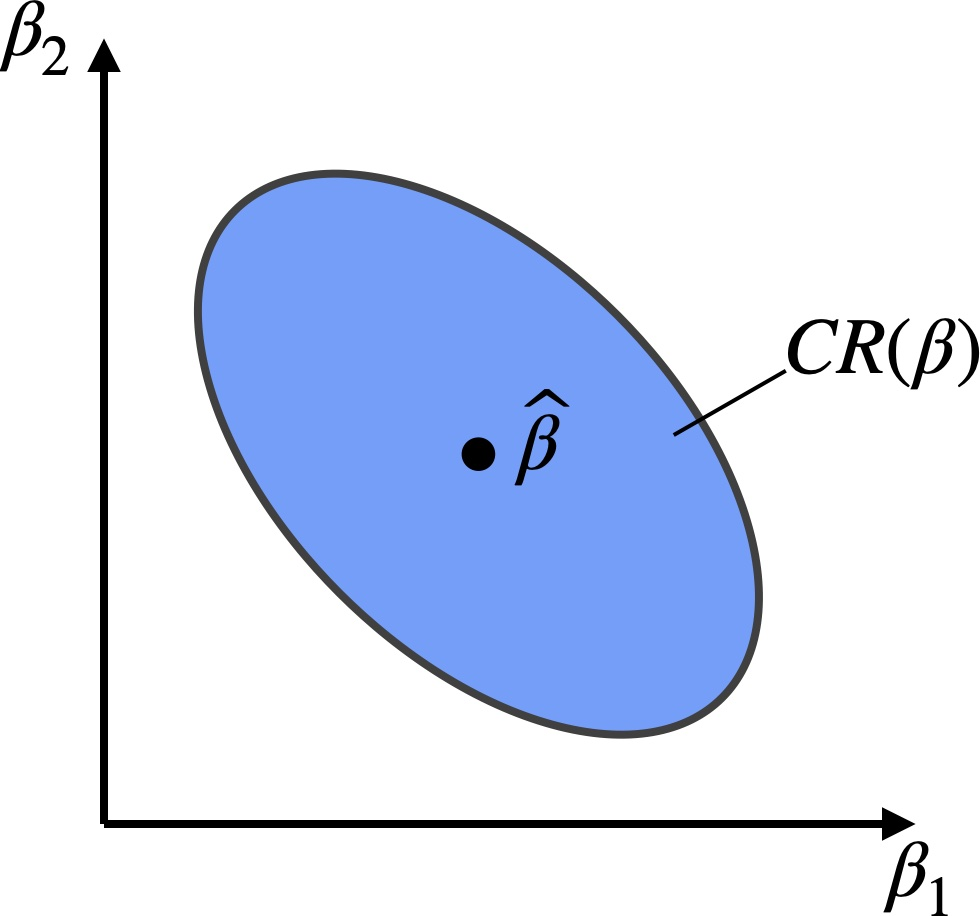
\includegraphics[width=0.4\textwidth,height=\textheight]{figures/confidence-regions.jpg}

}

\caption{\label{fig-confidence-region}Confidence region for
\(\boldsymbol \beta\).}

\end{figure}

\hypertarget{simultaneous-intervals}{%
\subsection{Simultaneous intervals}\label{simultaneous-intervals}}

As a byproduct of confidence regions for the multivariate
\(\boldsymbol \beta\), we can construct \emph{simultaneous intervals}
for univariate quantities. To motivate the definition of simultaneous
intervals, note that the intervals in
Section~\ref{sec-confidence-intervals-univariate} have \emph{pointwise
coverage}. For example, we have

\[
\mathbb{P}[\beta_j \in \text{CI}(\beta_j)] \geq 1-\alpha \quad \text{for each } j.
\]

or

\[
\mathbb{P}[\boldsymbol{\tilde x}^T \boldsymbol{\beta} \in \text{CI}(\boldsymbol{\tilde x}^T \boldsymbol{\beta})] \geq 1-\alpha \quad \text{for each } \boldsymbol{\tilde x}.
\]

Sometimes a stronger \emph{simultaneous coverage} guarantee is desired,
e.g.,

\begin{equation}\protect\hypertarget{eq-simultaneous-coordinatewise}{}{
\mathbb{P}[\beta_j \in \text{CI}^{\text{sim}}(\beta_j) \ \text{for each } j] \geq 1-\alpha
}\label{eq-simultaneous-coordinatewise}\end{equation}

or

\begin{equation}\protect\hypertarget{eq-simultaneous-contrasts}{}{
\mathbb{P}[\boldsymbol{\tilde x}^T \boldsymbol{\beta} \in \text{CI}^{\text{sim}}(\boldsymbol{\tilde x}^T \boldsymbol{\beta}) \ \text{for each } \boldsymbol{\tilde x}] \geq 1-\alpha.
}\label{eq-simultaneous-contrasts}\end{equation}

To obtain such simultaneous confidence intervals, we can leverage the
fact that the confidence region \(\text{CR}(\boldsymbol \beta)\) is for
the entire vector \(\boldsymbol{\beta}\). We can therefore define

\[
\text{CI}^{\text{sim}}(\beta_j) \equiv \{\beta_j: \boldsymbol{\beta} \in \text{CR}(\boldsymbol{\beta}) \}.
\]

Then, these confidence intervals will satisfy the simultaneous coverage
property (\ref{eq-simultaneous-coordinatewise}). We will obtain a more
explicit expression for \(\text{CI}^{\text{sim}}(\beta_j)\) shortly.

\begin{figure}

{\centering 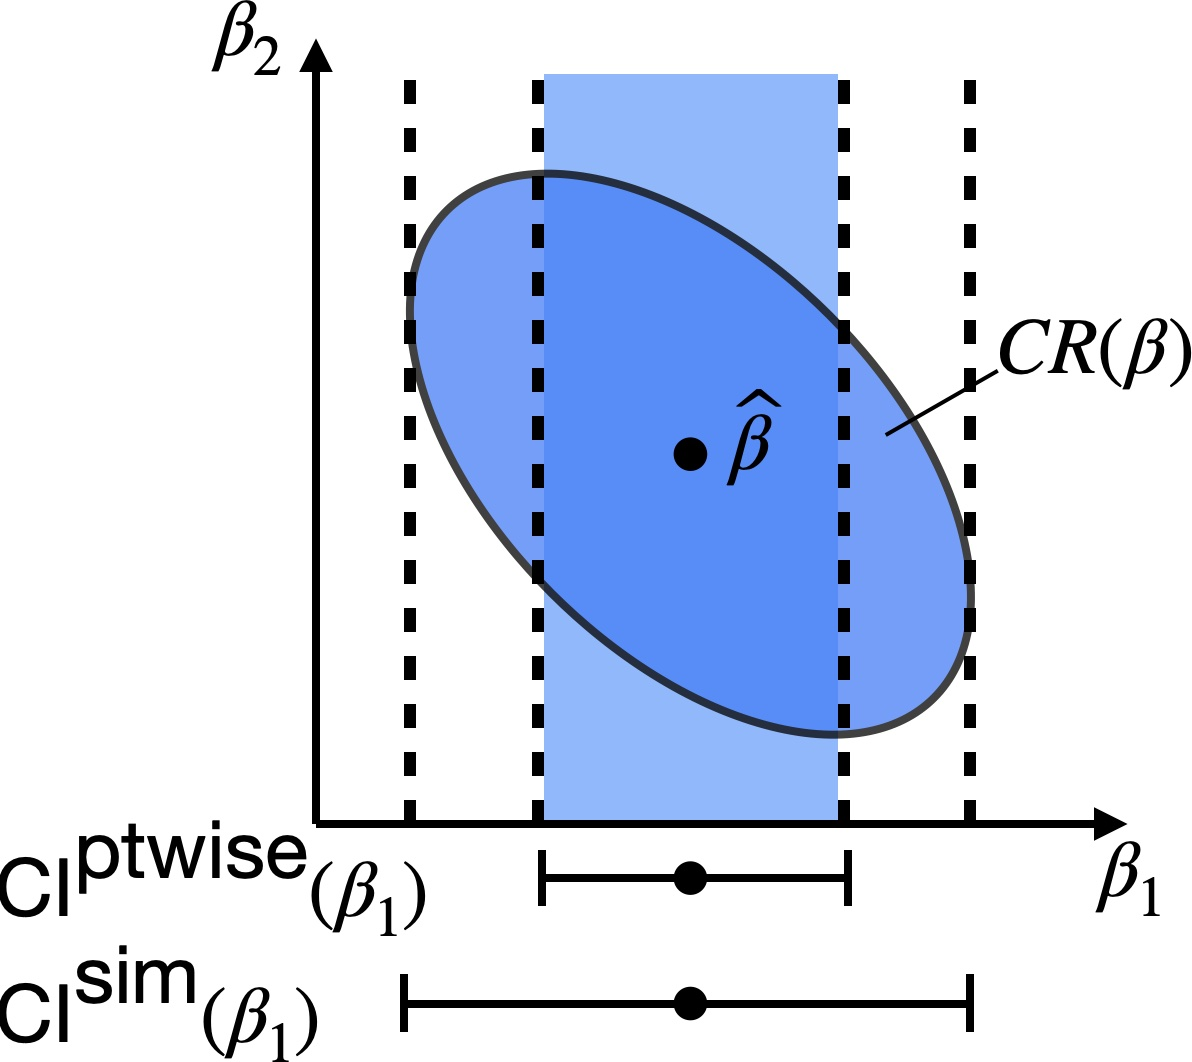
\includegraphics[width=0.4\textwidth,height=\textheight]{figures/confidence-regions-simultaneous-intervals.jpg}

}

\caption{\label{fig-confidence-region}Confidence region and simultaneous
and pointwise confidence intervals.}

\end{figure}

Similarly, we may define the simultaneous confidence regions

\[
\text{CI}^{\text{sim}}(\boldsymbol{\tilde x}^T \boldsymbol{\beta}) \equiv \{\boldsymbol{\tilde x}^T \boldsymbol{\beta}: \boldsymbol{\beta} \in \text{CR}(\boldsymbol{\beta})\}.
\]

Let us find a more explicit expression for the latter interval. For
notational ease, let us define
\(\boldsymbol{\Sigma} \equiv \boldsymbol{X}^T \boldsymbol{X}\). Then,
note that if \(\boldsymbol{\beta} \in \text{CR}(\boldsymbol{\beta})\),
then by the Cauchy-Schwarz inequality we have

\[
\begin{split}
(\boldsymbol{\tilde x}^T \boldsymbol{\widehat{\beta}}-\boldsymbol{\tilde x}^T \boldsymbol{\beta})^2 &= \|\boldsymbol{\tilde x}^T (\boldsymbol{\widehat{\beta}}-\boldsymbol{\beta})\|^2 \\
&= \|(\boldsymbol{\Sigma}^{-1/2}\boldsymbol{\tilde x})^T \boldsymbol{\Sigma}^{1/2}(\boldsymbol{\widehat{\beta}}-\boldsymbol{\beta})\|^2 \\
&\leq \|(\boldsymbol{\Sigma}^{-1/2}\boldsymbol{\tilde x})\|^2\|\boldsymbol{\Sigma}^{1/2}(\boldsymbol{\widehat{\beta}}-\boldsymbol{\beta})\|^2 \\
&\leq \boldsymbol{\tilde x}^T \boldsymbol{\Sigma}^{-1}\boldsymbol{\tilde x} p \widehat{\sigma}^2 F_{p, n-p}(1-\alpha),
\end{split}
\]

i.e.,

\begin{equation}\protect\hypertarget{eq-simultaneous-fit-se}{}{
\begin{split}
\boldsymbol{\tilde x}^T \boldsymbol{\beta} &\in \boldsymbol{\tilde x}^T \boldsymbol{\widehat{\beta}} \pm \widehat{\sigma} \sqrt{\boldsymbol{\tilde x}^T (\boldsymbol{X}^T \boldsymbol{X})^{-1}\boldsymbol{\tilde x}} \sqrt{pF_{p, n-p}(1-\alpha)} \\
&\equiv \boldsymbol{\tilde x}^T \boldsymbol{\widehat{\beta}} \pm \text{SE}(\boldsymbol{\tilde x}^T \boldsymbol{\widehat{\beta}})\cdot\sqrt{pF_{p, n-p}(1-\alpha)}.
\end{split}
}\label{eq-simultaneous-fit-se}\end{equation}

Defining the above interval as
\(\text{CI}^{\text{sim}}(\boldsymbol{\tilde x}^T \boldsymbol{\beta})\)
gives us the simultaneous coverage property
(\ref{eq-simultaneous-contrasts}). These simultaneous intervals are
called \emph{Working-Hotelling intervals}. Comparing to equation
(\ref{eq-pointwise-contrast-interval}), we see that the simultaneous
interval is the pointwise interval expanded by a factor of
\(\sqrt{pF_{p, n-p}(1-\alpha)}/t_{n-p}(1-\alpha/2)\). In the case of
simple linear regression, we can obtain simultaneous confidence bands
(Working-Hotelling bands) for the regression line.

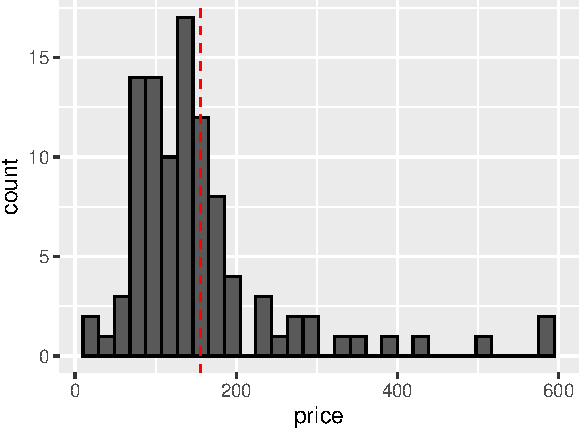
\includegraphics{confidence-intervals_files/figure-pdf/unnamed-chunk-2-1.pdf}

Specializing to the case
\(\boldsymbol{\tilde x} \equiv \boldsymbol{e_j}\), we get an expression
for the simultaneous intervals for each coordinate:

\begin{equation}\protect\hypertarget{eq-simultaneous-coordinatewise-se}{}{
\begin{split}
\text{CI}^{\text{sim}}(\beta_j) &\equiv \widehat \beta_j \pm \widehat{\sigma} \sqrt{(\boldsymbol{X}^T \boldsymbol{X})^{-1}_{jj}} \sqrt{pF_{p, n-p}(1-\alpha)} \\
&\equiv \text{SE}(\widehat \beta_j)\sqrt{pF_{p, n-p}(1-\alpha)},
\end{split}
}\label{eq-simultaneous-coordinatewise-se}\end{equation}

which again is the pointwise interval (\ref{eq-pointwise-interval-beta})
expanded by a factor of
\(\sqrt{pF_{p, n-p}(1-\alpha)}/t_{n-p}(1-\alpha/2)\).

\hypertarget{sec-practical-considerations}{%
\chapter{Practical considerations}\label{sec-practical-considerations}}

\hypertarget{practical-versus-statistical-significance}{%
\section{Practical versus statistical
significance}\label{practical-versus-statistical-significance}}

You can have a statistically significant effect that is not practically
significant. The hypothesis testing framework is most useful in the case
when the signal-to-noise ratio is relatively small. Otherwise,
constructing a confidence interval for the effect size is a more
meaningful approach.

\hypertarget{correlation-versus-causation-and-simpsons-paradox}{%
\section{Correlation versus causation, and Simpson's
paradox}\label{correlation-versus-causation-and-simpsons-paradox}}

Causation can be elusive for several reasons. One is reverse causation,
where it is not clear whether \(X\) causes \(Y\) or \(Y\) causes \(X\).
Another is confounding, where there is a third variable \(Z\) that
causes both \(X\) and \(Y\). For the latter reason, linear regression
coefficients can be sensitive to the choice of other predictors to
include and can be misleading if you omit important variables from the
regression. A special and sometimes overlooked case of this is
\emph{Simpson's paradox}, where an important discrete variable is
omitted. Consider the example in Figure~\ref{fig-simpson-paradox}.
Sometimes this discrete variable may seem benign, such as the year in
which the data was collected. Such variables might or might not be
measured.

\begin{figure}

{\centering 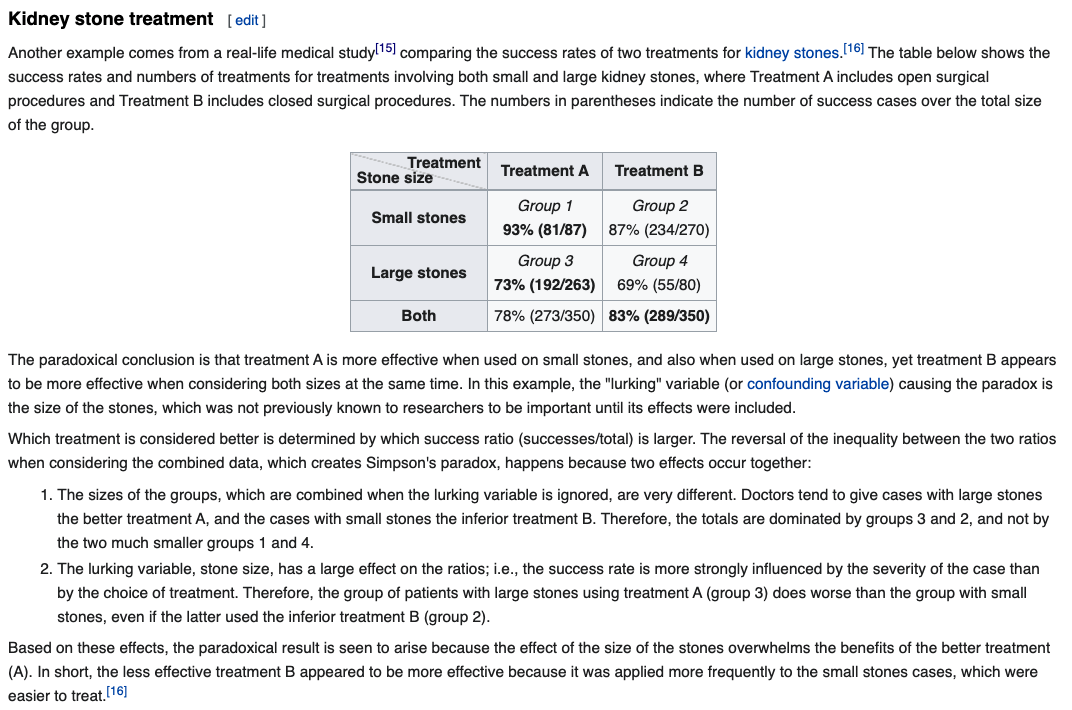
\includegraphics[width=1\textwidth,height=\textheight]{figures/kidney-stones.png}

}

\caption{\label{fig-simpson-paradox}An example of Simpson's paradox
(source: Wikipedia).}

\end{figure}

\hypertarget{dealing-with-correlated-predictors}{%
\section{Dealing with correlated
predictors}\label{dealing-with-correlated-predictors}}

It depends on the goal. If we're trying to tease apart effects of
correlated predictors, then we have no choice but to proceed as usual
despite lower power. Otherwise, we can test predictors in groups via the
\(F\)-test to get higher power at the cost of lower ``resolution.''
Sometimes, it is recommended to simply remove predictors that are
correlated with other predictors. This practice, however, is somewhat
arbitrary and not recommended.

\hypertarget{model-selection}{%
\section{Model selection}\label{model-selection}}

We need to ask ourselves: Why do we want to do model selection? It can
either be for prediction purposes or for inferential purposes. If it is
for prediction purposes, then we can apply cross-validation to select a
model and we don't need to think very hard about statistical
significance. If it is for inference, then we need to be more careful.
There are various classical model selection criteria (e.g., AIC, BIC),
but it is not entirely clear what statistical guarantee we are getting
for the resulting models. A simpler approach is to apply a \(t\)-test
for each variable in the model, apply a multiple testing correction to
the resulting \(p\)-values, and report the set of significant variables
and the associated guarantee. Re-fitting the linear regression after
model selection leads us into some dicey inferential territory due to
selection bias. This is the subject of ongoing research, and the jury is
still out on the best way of doing this.

\hypertarget{sec-r-demo-part-2}{%
\chapter{R demo}\label{sec-r-demo-part-2}}

\emph{See also Agresti 3.4.1, 3.4.3, Dunn and Smyth 2.6, 2.14}

Let's put into practice what we've learned in this chapter by analyzing
data about house prices.

\begin{Shaded}
\begin{Highlighting}[]
\FunctionTok{library}\NormalTok{(tidyverse)}
\FunctionTok{library}\NormalTok{(GGally)}

\NormalTok{houses\_data }\OtherTok{\textless{}{-}} \FunctionTok{read\_tsv}\NormalTok{(}\StringTok{"data/Houses.dat"}\NormalTok{)}
\NormalTok{houses\_data}
\end{Highlighting}
\end{Shaded}

\begin{verbatim}
# A tibble: 100 x 7
    case taxes  beds baths   new price  size
   <dbl> <dbl> <dbl> <dbl> <dbl> <dbl> <dbl>
 1     1  3104     4     2     0  280.  2048
 2     2  1173     2     1     0  146.   912
 3     3  3076     4     2     0  238.  1654
 4     4  1608     3     2     0  200   2068
 5     5  1454     3     3     0  160.  1477
 6     6  2997     3     2     1  500.  3153
 7     7  4054     3     2     0  266.  1355
 8     8  3002     3     2     1  290.  2075
 9     9  6627     5     4     0  587   3990
10    10   320     3     2     0   70   1160
# i 90 more rows
\end{verbatim}

\hypertarget{exploration-1}{%
\section{Exploration}\label{exploration-1}}

Let's first do a bit of exploration:

\begin{Shaded}
\begin{Highlighting}[]
\CommentTok{\# visualize distribution of housing prices, superimposing the mean}
\NormalTok{houses\_data }\SpecialCharTok{|\textgreater{}}
  \FunctionTok{ggplot}\NormalTok{(}\FunctionTok{aes}\NormalTok{(}\AttributeTok{x =}\NormalTok{ price)) }\SpecialCharTok{+}
  \FunctionTok{geom\_histogram}\NormalTok{(}\AttributeTok{color =} \StringTok{"black"}\NormalTok{, }\AttributeTok{bins =} \DecValTok{30}\NormalTok{) }\SpecialCharTok{+}
  \FunctionTok{geom\_vline}\NormalTok{(}\FunctionTok{aes}\NormalTok{(}\AttributeTok{xintercept =} \FunctionTok{mean}\NormalTok{(price)),}
    \AttributeTok{colour =} \StringTok{"red"}\NormalTok{,}
    \AttributeTok{linetype =} \StringTok{"dashed"}
\NormalTok{  )}
\end{Highlighting}
\end{Shaded}

\begin{figure}[H]

{\centering 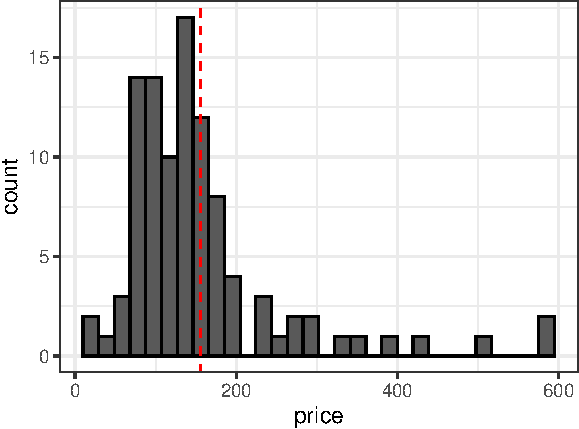
\includegraphics{r-demo-part-2_files/figure-pdf/unnamed-chunk-3-1.pdf}

}

\end{figure}

\begin{Shaded}
\begin{Highlighting}[]
\CommentTok{\# compare median and mean price}
\NormalTok{houses\_data }\SpecialCharTok{|\textgreater{}}
  \FunctionTok{summarise}\NormalTok{(}
    \AttributeTok{mean\_price =} \FunctionTok{mean}\NormalTok{(price),}
    \AttributeTok{median\_price =} \FunctionTok{median}\NormalTok{(price)}
\NormalTok{  )}
\end{Highlighting}
\end{Shaded}

\begin{verbatim}
# A tibble: 1 x 2
  mean_price median_price
       <dbl>        <dbl>
1       155.         133.
\end{verbatim}

\begin{Shaded}
\begin{Highlighting}[]
\CommentTok{\# create a pairs plot of continuous variables}
\NormalTok{houses\_data }\SpecialCharTok{|\textgreater{}}
  \FunctionTok{select}\NormalTok{(price, size, taxes) }\SpecialCharTok{|\textgreater{}}
  \FunctionTok{ggpairs}\NormalTok{()}
\end{Highlighting}
\end{Shaded}

\begin{figure}[H]

{\centering 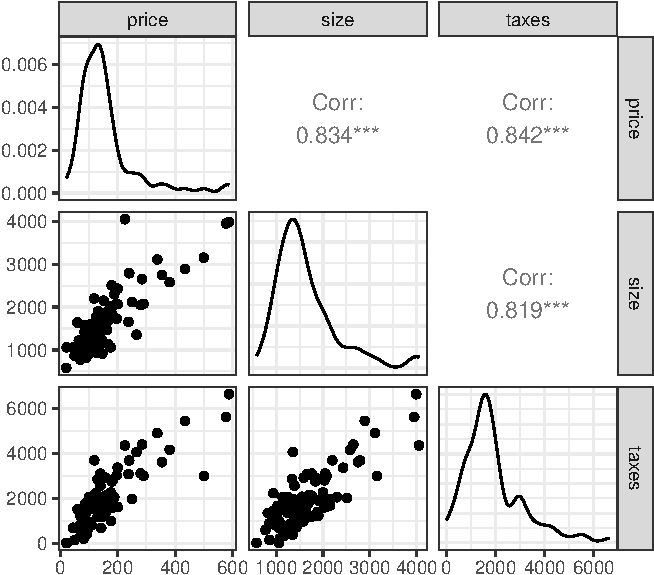
\includegraphics{r-demo-part-2_files/figure-pdf/unnamed-chunk-5-1.pdf}

}

\end{figure}

\begin{Shaded}
\begin{Highlighting}[]
\CommentTok{\# see how price relates to beds}
\NormalTok{houses\_data }\SpecialCharTok{|\textgreater{}}
  \FunctionTok{ggplot}\NormalTok{(}\FunctionTok{aes}\NormalTok{(}\AttributeTok{x =} \FunctionTok{factor}\NormalTok{(beds), }\AttributeTok{y =}\NormalTok{ price)) }\SpecialCharTok{+}
  \FunctionTok{geom\_boxplot}\NormalTok{(}\AttributeTok{fill =} \StringTok{"dodgerblue"}\NormalTok{)}
\end{Highlighting}
\end{Shaded}

\begin{figure}[H]

{\centering 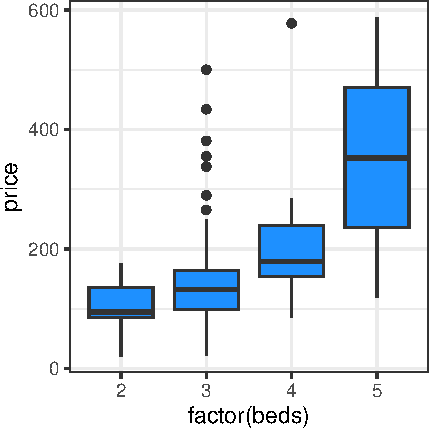
\includegraphics{r-demo-part-2_files/figure-pdf/unnamed-chunk-6-1.pdf}

}

\end{figure}

\begin{Shaded}
\begin{Highlighting}[]
\CommentTok{\# see how price relates to baths}
\NormalTok{houses\_data }\SpecialCharTok{|\textgreater{}}
  \FunctionTok{ggplot}\NormalTok{(}\FunctionTok{aes}\NormalTok{(}\AttributeTok{x =} \FunctionTok{factor}\NormalTok{(baths), }\AttributeTok{y =}\NormalTok{ price)) }\SpecialCharTok{+}
  \FunctionTok{geom\_boxplot}\NormalTok{(}\AttributeTok{fill =} \StringTok{"dodgerblue"}\NormalTok{)}
\end{Highlighting}
\end{Shaded}

\begin{figure}[H]

{\centering 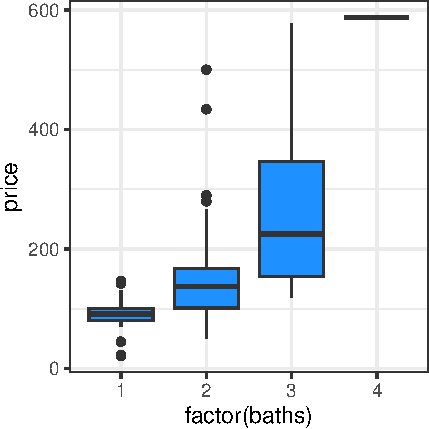
\includegraphics{r-demo-part-2_files/figure-pdf/unnamed-chunk-7-1.pdf}

}

\end{figure}

\begin{Shaded}
\begin{Highlighting}[]
\CommentTok{\# see how price relates to new}
\NormalTok{houses\_data }\SpecialCharTok{|\textgreater{}}
  \FunctionTok{ggplot}\NormalTok{(}\FunctionTok{aes}\NormalTok{(}\AttributeTok{x =} \FunctionTok{factor}\NormalTok{(new), }\AttributeTok{y =}\NormalTok{ price)) }\SpecialCharTok{+}
  \FunctionTok{geom\_boxplot}\NormalTok{(}\AttributeTok{fill =} \StringTok{"dodgerblue"}\NormalTok{)}
\end{Highlighting}
\end{Shaded}

\begin{figure}[H]

{\centering 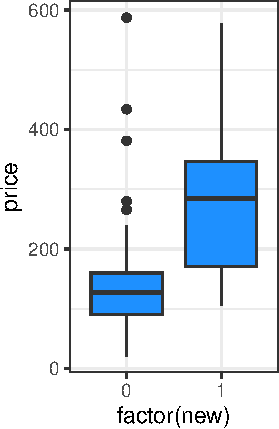
\includegraphics{r-demo-part-2_files/figure-pdf/unnamed-chunk-8-1.pdf}

}

\end{figure}

\hypertarget{hypothesis-testing}{%
\section{Hypothesis testing}\label{hypothesis-testing}}

Let's run a linear regression and interpret the summary. But first, we
must decide whether to model beds/baths as categorical or continuous? We
should probably model these as categorical, given the potentially
nonlinear trend observed in the box plots.

\begin{Shaded}
\begin{Highlighting}[]
\NormalTok{lm\_fit }\OtherTok{\textless{}{-}} \FunctionTok{lm}\NormalTok{(price }\SpecialCharTok{\textasciitilde{}} \FunctionTok{factor}\NormalTok{(beds) }\SpecialCharTok{+} \FunctionTok{factor}\NormalTok{(baths) }\SpecialCharTok{+}\NormalTok{ new }\SpecialCharTok{+}\NormalTok{ size,}
  \AttributeTok{data =}\NormalTok{ houses\_data}
\NormalTok{)}
\FunctionTok{summary}\NormalTok{(lm\_fit)}
\end{Highlighting}
\end{Shaded}

\begin{verbatim}

Call:
lm(formula = price ~ factor(beds) + factor(baths) + new + size, 
    data = houses_data)

Residuals:
     Min       1Q   Median       3Q      Max 
-179.306  -32.037   -2.899   19.115  152.718 

Coefficients:
                 Estimate Std. Error t value Pr(>|t|)    
(Intercept)     -19.26307   18.01344  -1.069 0.287730    
factor(beds)3   -16.46430   15.04669  -1.094 0.276749    
factor(beds)4   -12.48561   21.12357  -0.591 0.555936    
factor(beds)5  -101.14581   55.83607  -1.811 0.073366 .  
factor(baths)2    2.39872   15.44014   0.155 0.876885    
factor(baths)3   -0.70410   26.45512  -0.027 0.978825    
factor(baths)4  273.20079   83.65764   3.266 0.001540 ** 
new              66.94940   18.50445   3.618 0.000487 ***
size              0.10882    0.01234   8.822 7.46e-14 ***
---
Signif. codes:  0 '***' 0.001 '**' 0.01 '*' 0.05 '.' 0.1 ' ' 1

Residual standard error: 51.17 on 91 degrees of freedom
Multiple R-squared:  0.7653,    Adjusted R-squared:  0.7446 
F-statistic: 37.08 on 8 and 91 DF,  p-value: < 2.2e-16
\end{verbatim}

We can read off the test statistics and \(p\)-values for each variable
from the regression summary, as well as for the \(F\)-test against the
constant model from the bottom of the summary.

Let's use an \(F\)-test to assess whether the categorical \texttt{baths}
variable is important.

\begin{Shaded}
\begin{Highlighting}[]
\NormalTok{lm\_fit\_partial }\OtherTok{\textless{}{-}} \FunctionTok{lm}\NormalTok{(price }\SpecialCharTok{\textasciitilde{}} \FunctionTok{factor}\NormalTok{(beds) }\SpecialCharTok{+}\NormalTok{ new }\SpecialCharTok{+}\NormalTok{ size,}
  \AttributeTok{data =}\NormalTok{ houses\_data}
\NormalTok{)}
\FunctionTok{anova}\NormalTok{(lm\_fit\_partial, lm\_fit)}
\end{Highlighting}
\end{Shaded}

\begin{verbatim}
Analysis of Variance Table

Model 1: price ~ factor(beds) + new + size
Model 2: price ~ factor(beds) + factor(baths) + new + size
  Res.Df    RSS Df Sum of Sq      F   Pr(>F)   
1     94 273722                                
2     91 238289  3     35433 4.5104 0.005374 **
---
Signif. codes:  0 '***' 0.001 '**' 0.01 '*' 0.05 '.' 0.1 ' ' 1
\end{verbatim}

What if we had not coded \texttt{baths} as a factor?

\begin{Shaded}
\begin{Highlighting}[]
\NormalTok{lm\_fit\_not\_factor }\OtherTok{\textless{}{-}} \FunctionTok{lm}\NormalTok{(price }\SpecialCharTok{\textasciitilde{}} \FunctionTok{factor}\NormalTok{(beds) }\SpecialCharTok{+}\NormalTok{ baths }\SpecialCharTok{+}\NormalTok{ new }\SpecialCharTok{+}\NormalTok{ size,}
  \AttributeTok{data =}\NormalTok{ houses\_data}
\NormalTok{)}
\FunctionTok{anova}\NormalTok{(lm\_fit\_partial, lm\_fit\_not\_factor)}
\end{Highlighting}
\end{Shaded}

\begin{verbatim}
Analysis of Variance Table

Model 1: price ~ factor(beds) + new + size
Model 2: price ~ factor(beds) + baths + new + size
  Res.Df    RSS Df Sum of Sq      F Pr(>F)
1     94 273722                           
2     93 273628  1     94.33 0.0321 0.8583
\end{verbatim}

If we want to test for the equality of means across groups of a
categorical predictor, without adjusting for other variables, we can use
the ANOVA \(F\)-test. There are several equivalent ways of doing so:

\begin{Shaded}
\begin{Highlighting}[]
\CommentTok{\# just use the summary function}
\NormalTok{lm\_fit\_baths }\OtherTok{\textless{}{-}} \FunctionTok{lm}\NormalTok{(price }\SpecialCharTok{\textasciitilde{}} \FunctionTok{factor}\NormalTok{(baths), }\AttributeTok{data =}\NormalTok{ houses\_data)}
\FunctionTok{summary}\NormalTok{(lm\_fit\_baths)}
\end{Highlighting}
\end{Shaded}

\begin{verbatim}

Call:
lm(formula = price ~ factor(baths), data = houses_data)

Residuals:
    Min      1Q  Median      3Q     Max 
-146.44  -45.88   -7.89   22.22  352.01 

Coefficients:
               Estimate Std. Error t value Pr(>|t|)    
(Intercept)       90.21      19.51   4.624 1.17e-05 ***
factor(baths)2    57.68      21.72   2.656  0.00927 ** 
factor(baths)3   174.52      31.13   5.607 1.97e-07 ***
factor(baths)4   496.79      82.77   6.002 3.45e-08 ***
---
Signif. codes:  0 '***' 0.001 '**' 0.01 '*' 0.05 '.' 0.1 ' ' 1

Residual standard error: 80.44 on 96 degrees of freedom
Multiple R-squared:  0.3881,    Adjusted R-squared:  0.369 
F-statistic:  20.3 on 3 and 96 DF,  p-value: 2.865e-10
\end{verbatim}

\begin{Shaded}
\begin{Highlighting}[]
\CommentTok{\# use the anova function as before}
\NormalTok{lm\_fit\_const }\OtherTok{\textless{}{-}} \FunctionTok{lm}\NormalTok{(price }\SpecialCharTok{\textasciitilde{}} \DecValTok{1}\NormalTok{, }\AttributeTok{data =}\NormalTok{ houses\_data)}
\FunctionTok{anova}\NormalTok{(lm\_fit\_const, lm\_fit\_baths)}
\end{Highlighting}
\end{Shaded}

\begin{verbatim}
Analysis of Variance Table

Model 1: price ~ 1
Model 2: price ~ factor(baths)
  Res.Df     RSS Df Sum of Sq      F    Pr(>F)    
1     99 1015150                                  
2     96  621130  3    394020 20.299 2.865e-10 ***
---
Signif. codes:  0 '***' 0.001 '**' 0.01 '*' 0.05 '.' 0.1 ' ' 1
\end{verbatim}

\begin{Shaded}
\begin{Highlighting}[]
\CommentTok{\# use the aov function}
\NormalTok{aov\_fit }\OtherTok{\textless{}{-}} \FunctionTok{aov}\NormalTok{(price }\SpecialCharTok{\textasciitilde{}} \FunctionTok{factor}\NormalTok{(baths), }\AttributeTok{data =}\NormalTok{ houses\_data)}
\FunctionTok{summary}\NormalTok{(aov\_fit)}
\end{Highlighting}
\end{Shaded}

\begin{verbatim}
              Df Sum Sq Mean Sq F value   Pr(>F)    
factor(baths)  3 394020  131340    20.3 2.86e-10 ***
Residuals     96 621130    6470                     
---
Signif. codes:  0 '***' 0.001 '**' 0.01 '*' 0.05 '.' 0.1 ' ' 1
\end{verbatim}

We can also use an \(F\)-test to test for the presence of an interaction
with a multi-class categorical predictor.

\begin{Shaded}
\begin{Highlighting}[]
\NormalTok{lm\_fit\_interaction }\OtherTok{\textless{}{-}} \FunctionTok{lm}\NormalTok{(price }\SpecialCharTok{\textasciitilde{}}\NormalTok{ size }\SpecialCharTok{*} \FunctionTok{factor}\NormalTok{(beds), }\AttributeTok{data =}\NormalTok{ houses\_data)}
\FunctionTok{summary}\NormalTok{(lm\_fit\_interaction)}
\end{Highlighting}
\end{Shaded}

\begin{verbatim}

Call:
lm(formula = price ~ size * factor(beds), data = houses_data)

Residuals:
     Min       1Q   Median       3Q      Max 
-232.643  -25.938   -0.942   19.172  155.517 

Coefficients:
                     Estimate Std. Error t value Pr(>|t|)    
(Intercept)          50.12619   48.22282   1.039 0.301310    
size                  0.05037    0.04210   1.197 0.234565    
factor(beds)3      -103.85734   52.20373  -1.989 0.049620 *  
factor(beds)4      -143.90213   67.31359  -2.138 0.035185 *  
factor(beds)5      -507.88205  144.10191  -3.524 0.000663 ***
size:factor(beds)3    0.07589    0.04368   1.738 0.085633 .  
size:factor(beds)4    0.09234    0.04704   1.963 0.052638 .  
size:factor(beds)5    0.21147    0.05957   3.550 0.000609 ***
---
Signif. codes:  0 '***' 0.001 '**' 0.01 '*' 0.05 '.' 0.1 ' ' 1

Residual standard error: 53.35 on 92 degrees of freedom
Multiple R-squared:  0.7421,    Adjusted R-squared:  0.7225 
F-statistic: 37.81 on 7 and 92 DF,  p-value: < 2.2e-16
\end{verbatim}

\begin{Shaded}
\begin{Highlighting}[]
\NormalTok{lm\_fit\_size }\OtherTok{\textless{}{-}} \FunctionTok{lm}\NormalTok{(price }\SpecialCharTok{\textasciitilde{}}\NormalTok{ size }\SpecialCharTok{+} \FunctionTok{factor}\NormalTok{(beds), }\AttributeTok{data =}\NormalTok{ houses\_data)}
\FunctionTok{anova}\NormalTok{(lm\_fit\_size, lm\_fit\_interaction)}
\end{Highlighting}
\end{Shaded}

\begin{verbatim}
Analysis of Variance Table

Model 1: price ~ size + factor(beds)
Model 2: price ~ size * factor(beds)
  Res.Df    RSS Df Sum of Sq      F   Pr(>F)   
1     95 300953                                
2     92 261832  3     39121 4.5819 0.004905 **
---
Signif. codes:  0 '***' 0.001 '**' 0.01 '*' 0.05 '.' 0.1 ' ' 1
\end{verbatim}

Contrasts of regression coefficients can be tested using the
\texttt{glht()} function from the \texttt{multcomp} package.

\hypertarget{confidence-intervals}{%
\section{Confidence intervals}\label{confidence-intervals}}

We can construct pointwise confidence intervals for each coefficient
using \texttt{confint()}:

\begin{Shaded}
\begin{Highlighting}[]
\FunctionTok{confint}\NormalTok{(lm\_fit)}
\end{Highlighting}
\end{Shaded}

\begin{verbatim}
                       2.5 %      97.5 %
(Intercept)     -55.04455734  16.5184161
factor(beds)3   -46.35270691  13.4241025
factor(beds)4   -54.44498235  29.4737689
factor(beds)5  -212.05730801   9.7656895
factor(baths)2  -28.27123130  33.0686620
factor(baths)3  -53.25394742  51.8457394
factor(baths)4  107.02516067 439.3764122
new              30.19258305 103.7062177
size              0.08431972   0.1333284
\end{verbatim}

To create simultaneous confidence intervals, we need a somewhat more
manual approach. We start with the coefficients and standard errors:

\begin{Shaded}
\begin{Highlighting}[]
\FunctionTok{coef}\NormalTok{(}\FunctionTok{summary}\NormalTok{(lm\_fit))}
\end{Highlighting}
\end{Shaded}

\begin{verbatim}
                   Estimate  Std. Error     t value     Pr(>|t|)
(Intercept)     -19.2630706 18.01344052 -1.06937209 2.877304e-01
factor(beds)3   -16.4643022 15.04669172 -1.09421410 2.767490e-01
factor(beds)4   -12.4856067 21.12356937 -0.59107467 5.559357e-01
factor(beds)5  -101.1458092 55.83607248 -1.81147786 7.336590e-02
factor(baths)2    2.3987153 15.44014266  0.15535578 8.768849e-01
factor(baths)3   -0.7041040 26.45511871 -0.02661504 9.788251e-01
factor(baths)4  273.2007864 83.65764044  3.26570036 1.540093e-03
new              66.9494004 18.50445029  3.61801617 4.872475e-04
size              0.1088241  0.01233621  8.82151661 7.460814e-14
\end{verbatim}

Then we add lower and upper confidence interval endpoints based on the
formula (\ref{eq-simultaneous-coordinatewise-se}):

\begin{Shaded}
\begin{Highlighting}[]
\NormalTok{alpha }\OtherTok{\textless{}{-}} \FloatTok{0.05}
\NormalTok{n }\OtherTok{\textless{}{-}} \FunctionTok{nrow}\NormalTok{(houses\_data)}
\NormalTok{p }\OtherTok{\textless{}{-}} \FunctionTok{length}\NormalTok{(}\FunctionTok{coef}\NormalTok{(lm\_fit))}
\NormalTok{f\_quantile }\OtherTok{\textless{}{-}} \FunctionTok{qf}\NormalTok{(}\DecValTok{1} \SpecialCharTok{{-}}\NormalTok{ alpha, }\AttributeTok{df1 =}\NormalTok{ p, }\AttributeTok{df2 =}\NormalTok{ n }\SpecialCharTok{{-}}\NormalTok{ p)}
\FunctionTok{coef}\NormalTok{(}\FunctionTok{summary}\NormalTok{(lm\_fit)) }\SpecialCharTok{|\textgreater{}}
  \FunctionTok{as.data.frame}\NormalTok{() }\SpecialCharTok{|\textgreater{}}
  \FunctionTok{rownames\_to\_column}\NormalTok{(}\AttributeTok{var =} \StringTok{"Variable"}\NormalTok{) }\SpecialCharTok{|\textgreater{}}
  \FunctionTok{select}\NormalTok{(Variable, Estimate, }\StringTok{\textasciigrave{}}\AttributeTok{Std. Error}\StringTok{\textasciigrave{}}\NormalTok{) }\SpecialCharTok{|\textgreater{}}
  \FunctionTok{mutate}\NormalTok{(}
    \AttributeTok{CI\_lower =}\NormalTok{ Estimate }\SpecialCharTok{{-}} \StringTok{\textasciigrave{}}\AttributeTok{Std. Error}\StringTok{\textasciigrave{}} \SpecialCharTok{*} \FunctionTok{sqrt}\NormalTok{(p }\SpecialCharTok{*}\NormalTok{ f\_quantile),}
    \AttributeTok{CI\_upper =}\NormalTok{ Estimate }\SpecialCharTok{+} \StringTok{\textasciigrave{}}\AttributeTok{Std. Error}\StringTok{\textasciigrave{}} \SpecialCharTok{*} \FunctionTok{sqrt}\NormalTok{(p }\SpecialCharTok{*}\NormalTok{ f\_quantile)}
\NormalTok{  )}
\end{Highlighting}
\end{Shaded}

\begin{verbatim}
        Variable     Estimate  Std. Error      CI_lower    CI_upper
1    (Intercept)  -19.2630706 18.01344052  -95.38917389  56.8630327
2  factor(beds)3  -16.4643022 15.04669172  -80.05271036  47.1241059
3  factor(beds)4  -12.4856067 21.12356937 -101.75533960  76.7841262
4  factor(beds)5 -101.1458092 55.83607248 -337.11309238 134.8214739
5 factor(baths)2    2.3987153 15.44014266  -62.85244495  67.6498756
6 factor(baths)3   -0.7041040 26.45511871 -112.50535022 111.0971422
7 factor(baths)4  273.2007864 83.65764044  -80.34245635 626.7440292
8            new   66.9494004 18.50445029  -11.25174573 145.1505465
9           size    0.1088241  0.01233621    0.05669037   0.1609578
\end{verbatim}

Note that the simultaneous intervals are substantially larger.

To construct pointwise confidence intervals for the fit, we can use the
\texttt{predict()} function:

\begin{Shaded}
\begin{Highlighting}[]
\FunctionTok{predict}\NormalTok{(lm\_fit, }\AttributeTok{newdata =}\NormalTok{ houses\_data, }\AttributeTok{interval =} \StringTok{"confidence"}\NormalTok{) }\SpecialCharTok{|\textgreater{}} \FunctionTok{head}\NormalTok{()}
\end{Highlighting}
\end{Shaded}

\begin{verbatim}
        fit       lwr      upr
1 193.52176 165.22213 221.8214
2  79.98449  51.91430 108.0547
3 150.64507 122.28397 179.0062
4 191.71955 172.27396 211.1651
5 124.30169  81.34488 167.2585
6 376.74308 333.44559 420.0406
\end{verbatim}

To get pointwise prediction intervals, we switch \texttt{"confidence"}
to \texttt{"prediction"}:

\begin{Shaded}
\begin{Highlighting}[]
\FunctionTok{predict}\NormalTok{(lm\_fit, }\AttributeTok{newdata =}\NormalTok{ houses\_data, }\AttributeTok{interval =} \StringTok{"prediction"}\NormalTok{) }\SpecialCharTok{|\textgreater{}} \FunctionTok{head}\NormalTok{()}
\end{Highlighting}
\end{Shaded}

\begin{verbatim}
        fit       lwr      upr
1 193.52176  88.00908 299.0344
2  79.98449 -25.46688 185.4359
3 150.64507  45.11589 256.1743
4 191.71955  88.22951 295.2096
5 124.30169  13.95069 234.6527
6 376.74308 266.25901 487.2271
\end{verbatim}

To construct simultaneous confidence intervals for the fit or
predictions, we again need a slightly more manual approach. We call
\texttt{predict()} again, but this time asking it for the standard
errors rather than the confidence intervals:

\begin{Shaded}
\begin{Highlighting}[]
\NormalTok{predictions }\OtherTok{\textless{}{-}} \FunctionTok{predict}\NormalTok{(lm\_fit, }\AttributeTok{newdata =}\NormalTok{ houses\_data, }\AttributeTok{se.fit =} \ConstantTok{TRUE}\NormalTok{)}
\FunctionTok{head}\NormalTok{(predictions}\SpecialCharTok{$}\NormalTok{fit)}
\end{Highlighting}
\end{Shaded}

\begin{verbatim}
        1         2         3         4         5         6 
193.52176  79.98449 150.64507 191.71955 124.30169 376.74308 
\end{verbatim}

\begin{Shaded}
\begin{Highlighting}[]
\FunctionTok{head}\NormalTok{(predictions}\SpecialCharTok{$}\NormalTok{se.fit)}
\end{Highlighting}
\end{Shaded}

\begin{verbatim}
        1         2         3         4         5         6 
14.246855 14.131352 14.277804  9.789472 21.625709 21.797212 
\end{verbatim}

Now we can construct the simultaneous confidence intervals via the
formula (\ref{eq-simultaneous-fit-se}):

\begin{Shaded}
\begin{Highlighting}[]
\NormalTok{f\_quantile }\OtherTok{\textless{}{-}} \FunctionTok{qf}\NormalTok{(}\DecValTok{1} \SpecialCharTok{{-}}\NormalTok{ alpha, }\AttributeTok{df1 =}\NormalTok{ p, }\AttributeTok{df2 =}\NormalTok{ n }\SpecialCharTok{{-}}\NormalTok{ p)}
\FunctionTok{tibble}\NormalTok{(}
  \AttributeTok{lower =}\NormalTok{ predictions}\SpecialCharTok{$}\NormalTok{fit }\SpecialCharTok{{-}}\NormalTok{ predictions}\SpecialCharTok{$}\NormalTok{se.fit }\SpecialCharTok{*} \FunctionTok{sqrt}\NormalTok{(p }\SpecialCharTok{*}\NormalTok{ f\_quantile),}
  \AttributeTok{upper =}\NormalTok{ predictions}\SpecialCharTok{$}\NormalTok{fit }\SpecialCharTok{+}\NormalTok{ predictions}\SpecialCharTok{$}\NormalTok{se.fit }\SpecialCharTok{*} \FunctionTok{sqrt}\NormalTok{(p }\SpecialCharTok{*}\NormalTok{ f\_quantile)}
\NormalTok{)}
\end{Highlighting}
\end{Shaded}

\begin{verbatim}
# A tibble: 100 x 2
   lower upper
   <dbl> <dbl>
 1 133.   254.
 2  20.3  140.
 3  90.3  211.
 4 150.   233.
 5  32.9  216.
 6 285.   469.
 7  82.8  145.
 8 188.   331.
 9 371.   803.
10  57.3  128.
# i 90 more rows
\end{verbatim}

In the case of simple linear regression, we can plot these pointwise and
simultaneous confidence intervals as bands:

\begin{Shaded}
\begin{Highlighting}[]
\CommentTok{\# to produce confidence intervals for fits in general, use the predict() function}
\NormalTok{n }\OtherTok{\textless{}{-}} \FunctionTok{nrow}\NormalTok{(houses\_data)}
\NormalTok{p }\OtherTok{\textless{}{-}} \DecValTok{2}
\NormalTok{alpha }\OtherTok{\textless{}{-}} \FloatTok{0.05}
\NormalTok{lm\_fit }\OtherTok{\textless{}{-}} \FunctionTok{lm}\NormalTok{(price }\SpecialCharTok{\textasciitilde{}}\NormalTok{ size, }\AttributeTok{data =}\NormalTok{ houses\_data)}
\NormalTok{predictions }\OtherTok{\textless{}{-}} \FunctionTok{predict}\NormalTok{(lm\_fit, }\AttributeTok{se.fit =} \ConstantTok{TRUE}\NormalTok{)}
\NormalTok{t\_quantile }\OtherTok{\textless{}{-}} \FunctionTok{qt}\NormalTok{(}\DecValTok{1} \SpecialCharTok{{-}}\NormalTok{ alpha }\SpecialCharTok{/} \DecValTok{2}\NormalTok{, }\AttributeTok{df =}\NormalTok{ n }\SpecialCharTok{{-}}\NormalTok{ p)}
\NormalTok{f\_quantile }\OtherTok{\textless{}{-}} \FunctionTok{qf}\NormalTok{(}\DecValTok{1} \SpecialCharTok{{-}}\NormalTok{ alpha, }\AttributeTok{df1 =}\NormalTok{ p, }\AttributeTok{df2 =}\NormalTok{ n }\SpecialCharTok{{-}}\NormalTok{ p)}
\NormalTok{houses\_data }\SpecialCharTok{|\textgreater{}}
  \FunctionTok{mutate}\NormalTok{(}
    \AttributeTok{fit =}\NormalTok{ predictions}\SpecialCharTok{$}\NormalTok{fit,}
    \AttributeTok{se =}\NormalTok{ predictions}\SpecialCharTok{$}\NormalTok{se.fit,}
    \AttributeTok{ptwise\_width =}\NormalTok{ t\_quantile }\SpecialCharTok{*}\NormalTok{ se,}
    \AttributeTok{simultaneous\_width =} \FunctionTok{sqrt}\NormalTok{(p }\SpecialCharTok{*}\NormalTok{ f\_quantile) }\SpecialCharTok{*}\NormalTok{ se}
\NormalTok{  ) }\SpecialCharTok{|\textgreater{}}
  \FunctionTok{ggplot}\NormalTok{(}\FunctionTok{aes}\NormalTok{(}\AttributeTok{x =}\NormalTok{ size)) }\SpecialCharTok{+}
  \FunctionTok{geom\_point}\NormalTok{(}\FunctionTok{aes}\NormalTok{(}\AttributeTok{y =}\NormalTok{ price)) }\SpecialCharTok{+}
  \FunctionTok{geom\_line}\NormalTok{(}\FunctionTok{aes}\NormalTok{(}\AttributeTok{y =}\NormalTok{ fit), }\AttributeTok{color =} \StringTok{"blue"}\NormalTok{) }\SpecialCharTok{+}
  \FunctionTok{geom\_line}\NormalTok{(}\FunctionTok{aes}\NormalTok{(}\AttributeTok{y =}\NormalTok{ fit }\SpecialCharTok{+}\NormalTok{ ptwise\_width, }\AttributeTok{color =} \StringTok{"Pointwise"}\NormalTok{)) }\SpecialCharTok{+}
  \FunctionTok{geom\_line}\NormalTok{(}\FunctionTok{aes}\NormalTok{(}\AttributeTok{y =}\NormalTok{ fit }\SpecialCharTok{{-}}\NormalTok{ ptwise\_width, }\AttributeTok{color =} \StringTok{"Pointwise"}\NormalTok{)) }\SpecialCharTok{+}
  \FunctionTok{geom\_line}\NormalTok{(}\FunctionTok{aes}\NormalTok{(}\AttributeTok{y =}\NormalTok{ fit }\SpecialCharTok{+}\NormalTok{ simultaneous\_width, }\AttributeTok{color =} \StringTok{"Simultaneous"}\NormalTok{)) }\SpecialCharTok{+}
  \FunctionTok{geom\_line}\NormalTok{(}\FunctionTok{aes}\NormalTok{(}\AttributeTok{y =}\NormalTok{ fit }\SpecialCharTok{{-}}\NormalTok{ simultaneous\_width, }\AttributeTok{color =} \StringTok{"Simultaneous"}\NormalTok{)) }\SpecialCharTok{+}
  \FunctionTok{theme}\NormalTok{(}\AttributeTok{legend.title =} \FunctionTok{element\_blank}\NormalTok{(), }\AttributeTok{legend.position =} \StringTok{"bottom"}\NormalTok{)}
\end{Highlighting}
\end{Shaded}

\begin{figure}[H]

{\centering 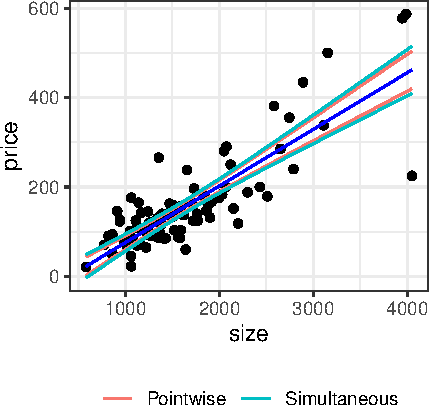
\includegraphics{r-demo-part-2_files/figure-pdf/unnamed-chunk-21-1.pdf}

}

\end{figure}

\hypertarget{predictor-competition-and-collaboration}{%
\section{Predictor competition and
collaboration}\label{predictor-competition-and-collaboration}}

Let's look at the power of detecting the association between
\texttt{price} and \texttt{beds}. We can imagine that \texttt{beds} and
\texttt{baths} are correlated:

\begin{Shaded}
\begin{Highlighting}[]
\NormalTok{houses\_data }\SpecialCharTok{|\textgreater{}}
  \FunctionTok{ggplot}\NormalTok{(}\FunctionTok{aes}\NormalTok{(}\AttributeTok{x =}\NormalTok{ beds, }\AttributeTok{y =}\NormalTok{ baths)) }\SpecialCharTok{+}
  \FunctionTok{geom\_count}\NormalTok{()}
\end{Highlighting}
\end{Shaded}

\begin{figure}[H]

{\centering 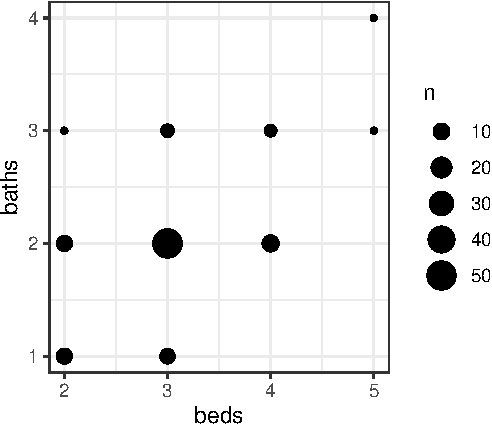
\includegraphics{r-demo-part-2_files/figure-pdf/unnamed-chunk-22-1.pdf}

}

\end{figure}

So let's see how significant \texttt{beds} is, with and without
\texttt{baths} in the model:

\begin{Shaded}
\begin{Highlighting}[]
\NormalTok{lm\_fit\_only\_beds }\OtherTok{\textless{}{-}} \FunctionTok{lm}\NormalTok{(price }\SpecialCharTok{\textasciitilde{}} \FunctionTok{factor}\NormalTok{(beds), }\AttributeTok{data =}\NormalTok{ houses\_data)}
\FunctionTok{summary}\NormalTok{(lm\_fit\_only\_beds)}
\end{Highlighting}
\end{Shaded}

\begin{verbatim}

Call:
lm(formula = price ~ factor(beds), data = houses_data)

Residuals:
    Min      1Q  Median      3Q     Max 
-234.35  -50.63  -15.69   24.56  365.86 

Coefficients:
              Estimate Std. Error t value Pr(>|t|)    
(Intercept)     105.94      21.48   4.931 3.43e-06 ***
factor(beds)3    44.69      24.47   1.827 0.070849 .  
factor(beds)4   105.70      32.35   3.268 0.001504 ** 
factor(beds)5   246.71      69.62   3.544 0.000611 ***
---
Signif. codes:  0 '***' 0.001 '**' 0.01 '*' 0.05 '.' 0.1 ' ' 1

Residual standard error: 93.65 on 96 degrees of freedom
Multiple R-squared:  0.1706,    Adjusted R-squared:  0.1447 
F-statistic: 6.583 on 3 and 96 DF,  p-value: 0.0004294
\end{verbatim}

\begin{Shaded}
\begin{Highlighting}[]
\NormalTok{lm\_fit\_only\_baths }\OtherTok{\textless{}{-}} \FunctionTok{lm}\NormalTok{(price }\SpecialCharTok{\textasciitilde{}} \FunctionTok{factor}\NormalTok{(baths), }\AttributeTok{data =}\NormalTok{ houses\_data)}
\NormalTok{lm\_fit\_beds\_baths }\OtherTok{\textless{}{-}} \FunctionTok{lm}\NormalTok{(price }\SpecialCharTok{\textasciitilde{}} \FunctionTok{factor}\NormalTok{(beds) }\SpecialCharTok{+} \FunctionTok{factor}\NormalTok{(baths), }\AttributeTok{data =}\NormalTok{ houses\_data)}
\FunctionTok{anova}\NormalTok{(lm\_fit\_only\_baths, lm\_fit\_beds\_baths)}
\end{Highlighting}
\end{Shaded}

\begin{verbatim}
Analysis of Variance Table

Model 1: price ~ factor(baths)
Model 2: price ~ factor(beds) + factor(baths)
  Res.Df    RSS Df Sum of Sq     F  Pr(>F)  
1     96 621130                             
2     93 572436  3     48693 2.637 0.05424 .
---
Signif. codes:  0 '***' 0.001 '**' 0.01 '*' 0.05 '.' 0.1 ' ' 1
\end{verbatim}

We see that the significance of \texttt{beds} dropped by two orders of
magnitude. This is an example of predictor competition.

On the other hand, note that the variable \texttt{new} is not very
correlated with \texttt{beds}:

\begin{Shaded}
\begin{Highlighting}[]
\NormalTok{lm\_fit }\OtherTok{\textless{}{-}} \FunctionTok{lm}\NormalTok{(new }\SpecialCharTok{\textasciitilde{}}\NormalTok{ beds, }\AttributeTok{data =}\NormalTok{ houses\_data)}
\FunctionTok{summary}\NormalTok{(lm\_fit)}
\end{Highlighting}
\end{Shaded}

\begin{verbatim}

Call:
lm(formula = new ~ beds, data = houses_data)

Residuals:
     Min       1Q   Median       3Q      Max 
-0.15762 -0.11000 -0.11000 -0.08619  0.91381 

Coefficients:
            Estimate Std. Error t value Pr(>|t|)
(Intercept)  0.03857    0.14950   0.258    0.797
beds         0.02381    0.04871   0.489    0.626

Residual standard error: 0.3157 on 98 degrees of freedom
Multiple R-squared:  0.002432,  Adjusted R-squared:  -0.007747 
F-statistic: 0.2389 on 1 and 98 DF,  p-value: 0.6261
\end{verbatim}

but we know it has a substantial impact on \texttt{price}. Let's look at
the significance of the test that \texttt{beds} is not important when we
add \texttt{new} to the model.

\begin{Shaded}
\begin{Highlighting}[]
\NormalTok{lm\_fit\_only\_new }\OtherTok{\textless{}{-}} \FunctionTok{lm}\NormalTok{(price }\SpecialCharTok{\textasciitilde{}}\NormalTok{ new, }\AttributeTok{data =}\NormalTok{ houses\_data)}
\NormalTok{lm\_fit\_beds\_new }\OtherTok{\textless{}{-}} \FunctionTok{lm}\NormalTok{(price }\SpecialCharTok{\textasciitilde{}}\NormalTok{ new }\SpecialCharTok{+} \FunctionTok{factor}\NormalTok{(beds), }\AttributeTok{data =}\NormalTok{ houses\_data)}
\FunctionTok{anova}\NormalTok{(lm\_fit\_only\_new, lm\_fit\_beds\_new)}
\end{Highlighting}
\end{Shaded}

\begin{verbatim}
Analysis of Variance Table

Model 1: price ~ new
Model 2: price ~ new + factor(beds)
  Res.Df    RSS Df Sum of Sq      F    Pr(>F)    
1     98 787781                                  
2     95 619845  3    167936 8.5795 4.251e-05 ***
---
Signif. codes:  0 '***' 0.001 '**' 0.01 '*' 0.05 '.' 0.1 ' ' 1
\end{verbatim}

Adding \texttt{new} to the model made the \(p\)-value more significant
by a factor of 10. This is an example of predictor collaboration.

\part{Linear models: Misspecification}

In our discussion of linear model inference in Unit 2, we assumed the
normal linear model throughout:

\[
\boldsymbol{y} = \boldsymbol{X} \boldsymbol{\beta} + \boldsymbol{\epsilon}, \quad \text{where} \ \boldsymbol{\epsilon} \sim N(\boldsymbol{0}, \sigma^2 \boldsymbol{I}_n).
\]

In this unit, we will discuss what happens when this model is
misspecified:

\begin{itemize}
\tightlist
\item
  \textbf{Non-normality} (Section~\ref{sec-non-normality}):
  \(\boldsymbol{\epsilon} \sim (0, \sigma^2 \boldsymbol{I}_n)\) but not
  \(N(0, \sigma^2 \boldsymbol{I}_n)\).
\item
  \textbf{Heteroskedastic and/or correlated errors}
  (Section~\ref{sec-heteroskedasticity}):
  \(\boldsymbol{\epsilon} \sim (0, \boldsymbol{\Sigma})\), where
  \(\boldsymbol{\Sigma} \neq \sigma^2 \boldsymbol{I}\). This includes
  the case of heteroskedastic errors (\(\boldsymbol{\Sigma}\) is
  diagonal but not a constant multiple of the identity) and correlated
  errors (\(\boldsymbol{\Sigma}\) is not diagonal).
\item
  \textbf{Model bias} (Section~\ref{sec-model-bias}): It is not the case
  that
  \(\mathbb{E}[\boldsymbol{y}] = \boldsymbol{X} \boldsymbol{\beta}\) for
  some \(\boldsymbol{\beta} \in \mathbb{R}^p\).
\item
  \textbf{Outliers} (Section~\ref{sec-outliers}): For one or more \(i\),
  it is not the case that
  \(y_i \sim N(\boldsymbol{x}_{i*}^T \boldsymbol{\beta}, \sigma^2)\).
\end{itemize}

For each type of misspecification, we will discuss its origins,
consequences, detection, and fixes
(Section~\ref{sec-non-normality}-Section~\ref{sec-outliers}). We then
discuss methodological approaches to address model misspecification,
including asymptotic robust inference methods
(Chapter~\ref{sec-asymptotic-methods}), the bootstrap
(Chapter~\ref{sec-bootstrap}), the permutation test
(Chapter~\ref{sec-permutation-test}), and robust estimation
(Chapter~\ref{sec-robust-estimation}). We conclude with an R demo
(Chapter~\ref{sec-R-demo-misspecification}).

\hypertarget{overview}{%
\chapter{Overview}\label{overview}}

\hypertarget{sec-non-normality}{%
\section{Non-normality}\label{sec-non-normality}}

\hypertarget{origin}{%
\subsection{Origin}\label{origin}}

Non-normality occurs when the distribution of \(y|\boldsymbol{x}\) is
either skewed or has heavier tails than the normal distribution. This
may happen, for example, if there is some discreteness in \(y\).

\hypertarget{consequences}{%
\subsection{Consequences}\label{consequences}}

Non-normality is the most benign of linear model misspecifications.
While we derived linear model inferences under the normality assumption,
all the corresponding statements hold asymptotically without this
assumption. Recall Homework 2 Question 1, or take for example the
simpler problem of estimating the mean \(\mu\) of a distribution based
on \(n\) samples from it: We can test \(H_0: \mu = 0\) and build a
confidence interval for \(\mu\) even if the underlying distribution is
not normal. So if \(n\) is relatively large and \(p\) is relatively
small, you need not worry too much. If \(n\) is small and the errors are
highly skewed or heavy-tailed, we may have issues with incorrect
standard errors.

\hypertarget{detection}{%
\subsection{Detection}\label{detection}}

Non-normality is a property of the error terms \(\epsilon_i\). We do not
observe these directly, but we can approximate them using the residuals:

\[
\widehat{\epsilon}_i = y_i - \boldsymbol{x}_{i*}^T \boldsymbol{\widehat{\beta}}.
\]

Recall from equation (\ref{eq-fit-and-error-dist}) that
\(\text{Var}[\boldsymbol{\widehat{\epsilon}}] = \sigma^2(\boldsymbol{I} - \boldsymbol{H})\).
Letting \(h_i\) be the \(i\)th diagonal entry of \(\boldsymbol{H}\), it
follows that \(\widehat{\epsilon}_i \sim (0, \sigma^2(1-h_i))\). The
\emph{standardized residuals} are defined as:

\begin{equation}\protect\hypertarget{eq-standardized-residuals}{}{
r_i = \frac{\widehat{\epsilon}_i}{\widehat{\sigma} \sqrt{1-h_i}}.
}\label{eq-standardized-residuals}\end{equation}

Under normality, we would expect \(r_i \overset{\cdot}{\sim} N(0,1)\).
We can therefore assess normality by producing a histogram or normal
QQ-plot of these residuals.

\includegraphics{misspecification-overview_files/figure-pdf/unnamed-chunk-1-1.pdf}

\hypertarget{fixes}{%
\subsection{Fixes}\label{fixes}}

As mentioned above, non-normality is not necessarily a problem that
needs to be fixed, except in small samples. In small samples (but not
too small!), we can apply the residual bootstrap for robust standard
error computation and/or robust hypothesis testing.

\hypertarget{sec-heteroskedasticity}{%
\section{Heteroskedastic and correlated
errors}\label{sec-heteroskedasticity}}

\hypertarget{origin-1}{%
\subsection{Origin}\label{origin-1}}

\textbf{Heteroskedasticity} can arise as follows. Suppose each
observation \(y_i\) is actually the average of \(n_i\) underlying
observations, each with variance \(\sigma^2\). Then, the variance of
\(y_i\) is \(\sigma^2/n_i\), which will differ across \(i\) if \(n_i\)
differ. It is also common to see the variance of a distribution increase
as the mean increases (as in Figure~\ref{fig-heteroskedasticity}),
whereas for a linear model the variance of \(y\) stays constant as the
mean of \(y\) varies.

\textbf{Correlated errors} can arise when observations have group,
spatial, or temporal structure. Below are examples:

\begin{itemize}
\tightlist
\item
  \textbf{Group/clustered structure}: We have 10 samples
  \((\boldsymbol{x}_{i*}, y_i)\) each from 100 schools.
\item
  \textbf{Spatial structure}: We have 100 soil samples from a
  \(10\times10\) grid on a 1km \(\times\) 1km field.
\item
  \textbf{Temporal structure}: We have 366 COVID positivity rate
  measurements, one from each day of the year 2020.
\end{itemize}

The issue arises because there are common sources of variation among
samples that are in the same group or spatially/temporally close to one
another.

\hypertarget{consequences-1}{%
\subsection{Consequences}\label{consequences-1}}

All normal linear model inference from Unit 2 hinges on the assumption
that
\(\boldsymbol{\epsilon} \sim N(\boldsymbol{0}, \sigma^2 \boldsymbol{I})\).
If instead of \(\sigma^2 \boldsymbol{I}\) we have
\(\text{Var}[\boldsymbol{\epsilon}] = \boldsymbol{\Sigma}\) for some
matrix \(\boldsymbol{\Sigma}\), then we may suffer two consequences:
wrong inference (in terms of confidence interval coverage and hypothesis
test levels) and inefficient inference (in terms of confidence interval
width and hypothesis test power). One way of seeing the consequence of
heteroskedasticity for confidence interval coverage is the width of
prediction intervals; see Figure~\ref{fig-heteroskedasticity} for
intuition.

\begin{figure}

{\centering 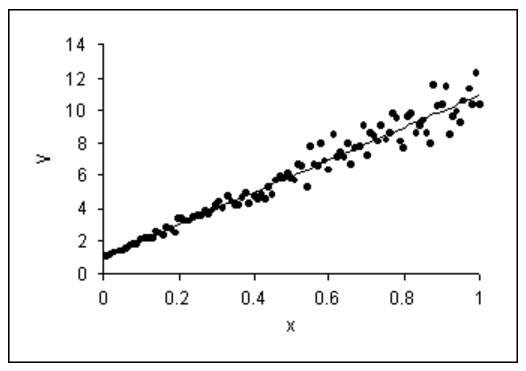
\includegraphics[width=0.6\textwidth,height=\textheight]{figures/heteroskedasticity.png}

}

\caption{\label{fig-heteroskedasticity}Heteroskedasticity in a simple
bivariate linear model (image source:
\href{http://www3.wabash.edu/econometrics/EconometricsBook/chap19.htm}{source}).}

\end{figure}

Like with heteroskedastic errors, correlated errors can cause invalid
standard errors. In particular, positively correlated errors typically
cause standard errors to be smaller than they should be, leading to
inflated Type-I error rates. For intuition, consider estimating the mean
of a distribution based on \(n\) samples. Consider the cases when these
samples are independent, compared to when they are perfectly correlated.
The effective sample size in the former case is \(n\) and in the latter
case is 1.

\hypertarget{detection-1}{%
\subsection{Detection}\label{detection-1}}

Heteroskedasticity is usually assessed via the \emph{residual plot}
(Figure~\ref{fig-residual-plots}). In this plot, the standardized
residuals \(r_i\) (\ref{eq-standardized-residuals}) are plotted against
the fitted values \(\widehat{\mu}_i\). In the absence of
heteroskedasticity, the spread of the points around the origin should be
roughly constant as a function of \(\widehat{\mu}\)
(Figure~\ref{fig-residual-plots}(a)). A common sign of
heteroskedasticity is the fan shape where variance increases as a
function of \(\widehat{\mu}\) (Figure~\ref{fig-residual-plots}(c)).

\begin{figure}

{\centering 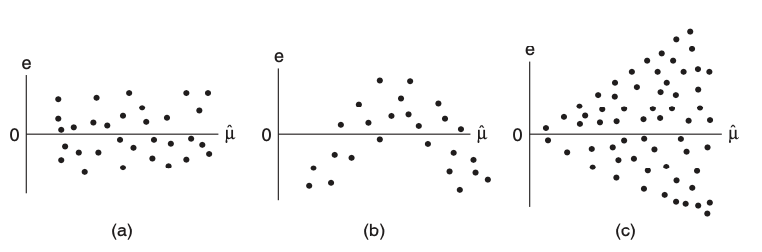
\includegraphics[width=1\textwidth,height=\textheight]{figures/residual-plots.png}

}

\caption{\label{fig-residual-plots}Residuals plotted against
linear-model fitted values that reflect (a) model adequacy, (b)
quadratic rather than linear relationship, and (c) nonconstant variance
(image source: Agresti Figure 2.8).}

\end{figure}

Residual plots once again come in handy to detect correlated errors.
Instead of plotting the standardized residuals against the fitted
values, we should plot the residuals against whatever variables we think
might explain variation in the response that the regression does not
account for. In the presence of group structures, we can plot residuals
versus group (via a boxplot); in the presence of spatial or temporal
structure, we can plot residuals as a function of space or time. If the
residuals show a dependency on these variables, this suggests they are
correlated. This dependency can be checked via formal means as well,
e.g., via an ANOVA test in the case of groups or by estimating the
autocorrelation function in the case of temporal structure.

\hypertarget{sec-model-bias}{%
\section{Model bias}\label{sec-model-bias}}

\hypertarget{origin-2}{%
\subsection{Origin}\label{origin-2}}

Model bias arises when predictors are left out of the regression model:

\begin{equation}\protect\hypertarget{eq-confounding}{}{
\text{assumed model: } \boldsymbol{y} = \boldsymbol{X} \boldsymbol{\beta} + \boldsymbol{\epsilon}; \quad \text{actual model: } \boldsymbol{y} = \boldsymbol{X} \boldsymbol{\beta} + \boldsymbol{Z} \boldsymbol{\gamma} + \boldsymbol{\epsilon}.
}\label{eq-confounding}\end{equation}

We may not always know about or measure all the variables that impact a
response \(\boldsymbol{y}\).

Model bias can also arise when the predictors do not impact the response
on the linear scale. For example:

\begin{equation}\protect\hypertarget{eq-wrong-scale}{}{
\text{assumed model: } \mathbb{E}[\boldsymbol{y}] = \boldsymbol{X} \boldsymbol{\beta}; \quad \text{actual model: } g(\mathbb{E}[\boldsymbol{y}]) = \boldsymbol{X} \boldsymbol{\beta}.
}\label{eq-wrong-scale}\end{equation}

\hypertarget{consequences-2}{%
\subsection{Consequences}\label{consequences-2}}

In cases of model bias, the parameters \(\boldsymbol{\beta}\) in the
assumed linear model lose their meanings. The least squares estimate
\(\boldsymbol{\widehat{\beta}}\) will be a biased estimate for the
parameter we probably actually want to estimate. In the case
(\ref{eq-confounding}) when predictors are left out of the regression
model, these additional predictors \(\boldsymbol{Z}\) will act as
confounders and create bias in \(\boldsymbol{\widehat{\beta}}\) as an
estimate of the \(\boldsymbol{\beta}\) parameters in the true model,
unless \(\boldsymbol{X}^T \boldsymbol{Z} = 0\). As discussed in Unit 2,
this can lead to misleading conclusions.

\hypertarget{detection-2}{%
\subsection{Detection}\label{detection-2}}

Similarly to the detection of correlated errors, we can try to identify
model bias by plotting the standardized residuals against predictors
that may have been left out of the model. A good place to start is to
plot standardized residuals against the predictors \(\boldsymbol{X}\)
(one at a time) that are in the model, since nonlinear transformations
of these might have been left out. In this case, you would see something
like Figure~\ref{fig-residual-plots}(b).

It is possible to formally test for model bias in cases when we have
repeated observations of the response for each value of the predictor
vector. In particular, suppose that
\(\boldsymbol{x}_{i*} = \boldsymbol{x}_c\) for \(c = c(i)\) and
predictor vectors
\(\boldsymbol{x}_1, \dots, \boldsymbol{x}_C \in \mathbb{R}^p\). Then,
consider testing the following hypothesis:

\[
H_0: y_i = \boldsymbol{x}_{i*}^T \boldsymbol{\beta} + \epsilon_i \quad \text{versus} \quad H_1: y_i = \beta_{c(i)} + \epsilon_i.
\]

The model under \(H_0\) (the linear model) is nested in the model for
\(H_1\) (the saturated model), and we can test this hypothesis using an
\(F\)-test called the \emph{lack of fit \(F\)-test}.

\hypertarget{overview-of-fixes}{%
\subsection{Overview of fixes}\label{overview-of-fixes}}

To fix model bias in the case (\ref{eq-confounding}), ideally we would
identify the missing predictors \(\boldsymbol{Z}\) and add them to the
regression model. This may not always be feasible or possible. To fix
model bias in the case (\ref{eq-wrong-scale}), it is sometimes advocated
to find a transformation \(g\) (e.g., a square root or a logarithm) of
\(\boldsymbol{y}\) such that
\(\mathbb{E}[g(\boldsymbol{y})] = \boldsymbol{X} \boldsymbol{\beta}\).
However, a better solution is to use a \emph{generalized linear model},
which we will discuss starting in Unit 4.

\hypertarget{sec-outliers}{%
\section{Outliers}\label{sec-outliers}}

\hypertarget{origin-3}{%
\subsection{Origin}\label{origin-3}}

Outliers often arise due to measurement or data entry errors. An
observation can be an outlier in \(\boldsymbol{x}\), in \(y\), or both.

\hypertarget{consequences-3}{%
\subsection{Consequences}\label{consequences-3}}

An outlier can have the effect of biasing the estimate
\(\boldsymbol{\widehat{\beta}}\). This occurs when an observation has
outlying \(\boldsymbol{x}\) as well as outlying \(y\).

\hypertarget{detection-3}{%
\subsection{Detection}\label{detection-3}}

There are a few measures associated with an observation that can be used
to detect outliers, though none are perfect. The first quantity is
called the \emph{leverage}, defined as:

\[
\text{leverage of observation } i \equiv \text{corr}^2(y_i, \widehat{\mu}_i).
\]

This quantity measures the extent to which the fitted value
\(\widehat{\mu}_i\) is sensitive to the (noise in the) observation
\(y_i\). It can be derived that:

\[
\text{leverage of observation } i = h_i,
\]

which is the \(i\)th diagonal element of the hat matrix
\(\boldsymbol{H}\). This is related to the fact that
\(\text{Var}[\widehat{\epsilon}_i] = \sigma^2(1-h_i)\). The larger the
leverage, the smaller the variance of the residual, so the closer the
line passes to the \(i\)th observation. The leverage of an observation
is larger to the extent that \(\boldsymbol{x}_{i*}\) is far from
\(\boldsymbol{\bar{x}}\). For example, in the bivariate linear model
\(y_i = \beta_0 + \beta_1 x_i + \epsilon_i\),

\[
h_i = \frac{1}{n} + \frac{(x_i - \bar{x})^2}{\sum_{i' = 1}^n (x_{i'} - \bar{x})^2}.
\]

Note that the average of the leverages is:

\[
\frac{1}{n}\sum_{i = 1}^n h_i = \frac{1}{n}\text{trace}(\boldsymbol{H}) = \frac{p}{n}.
\]

An observation's leverage is considered large if it is significantly
larger than this, e.g., three times larger.

Note that the leverage is not a function of \(y_i\), so a high-leverage
point might or might not be an outlier in \(y_i\) and therefore might or
might not have a strong impact on the regression. To assess more
directly whether an observation is \emph{influential}, we can compare
the least squares fits with and without that observation. To this end,
we define the \emph{Cook's distance}:

\[
D_i = \frac{\sum_{i' = 1}^n (\widehat{\mu}_{i'} - \widehat{\mu}^{\text{-}i}_{i'})^2}{p\widehat{\sigma}^2},
\]

where
\(\widehat{\mu}^{\text{-}i}_{i'} = \boldsymbol{x}_{i*}^T \boldsymbol{\widehat{\beta}}^{\text{-}i}\)
and \(\boldsymbol{\widehat{\beta}}^{\text{-}i}\) is the least squares
estimate based on
\((\boldsymbol{X}_{\text{-}i,*}, \boldsymbol{y}_{\text{-}i})\). An
observation is considered influential if it has Cook's distance greater
than one.

There is a connection between Cook's distance and leverage:

\[
D_i = \left(\frac{y_i - \widehat{\mu}_i}{\widehat{\sigma} \sqrt{1-h_{ii}}}\right)^2 \cdot \frac{h_{ii}}{p(1-h_{ii})}.
\]

We recognize the first term as the standardized residual; therefore a
point is influential if its residual and leverage are large.

Note that Cook's distance may not successfully identify outliers. For
example, if there are groups of outliers, then they will \emph{mask}
each other in the calculation of Cook's distance.

\hypertarget{overview-of-fixes-1}{%
\subsection{Overview of fixes}\label{overview-of-fixes-1}}

If outliers can be detected, then the fix is to remove them from the
regression. But, we need to be careful. Definitively determining whether
observations are outliers can be tricky. Outlier detection can even be
used as a way to commit fraud with data, as now-defunct blood testing
start-up
\href{https://arstechnica.com/tech-policy/2021/09/cherry-picking-data-was-routine-practice-at-theranos-former-lab-worker-says/}{Theranos}
is alleged to have done. As an alternative to removing outliers, we can
fit estimators \(\boldsymbol{\widehat{\beta}}\) that are less sensitive
to outliers; see Chapter~\ref{sec-robust-estimation}.

\hypertarget{sec-asymptotic-methods}{%
\chapter{Asymptotic methods}\label{sec-asymptotic-methods}}

In this section, we present a set of asymptotic methods for fixing
heteroskedastic or correlated errors, in the setting that
\begin{equation}\protect\hypertarget{eq-correlated-errors}{}{
\boldsymbol{y} \sim N(\boldsymbol{X} \boldsymbol{\beta}, \boldsymbol{\Sigma}).
}\label{eq-correlated-errors}\end{equation} These methods are based on
estimating \(\boldsymbol{\Sigma}\); they use this estimate to either (i)
build a better estimate \(\boldsymbol{\widehat{\beta}}\)
(Section~\ref{sec-better-estimate}) or (ii) build better standard errors
for the least squares estimate
(Section~\ref{sec-better-standard-errors}). We discuss these two
approaches in turn, followed by how to carry out inference based on the
resulting estimates (Section~\ref{sec-sandwich-inference}).

\hypertarget{sec-better-estimate}{%
\section{\texorpdfstring{Methods that build a better estimate of
\(\boldsymbol{\beta}\)}{Methods that build a better estimate of \textbackslash boldsymbol\{\textbackslash beta\}}}\label{sec-better-estimate}}

\hypertarget{generalized-least-squares}{%
\subsection{Generalized least squares}\label{generalized-least-squares}}

Let us premultiply \(\boldsymbol y\) by \(\boldsymbol \Sigma^{-1/2}\) to
obtain \[
\boldsymbol \Sigma^{-1/2} \boldsymbol y \sim N(\boldsymbol \Sigma^{-1/2} \boldsymbol X \boldsymbol \beta, \boldsymbol I).
\] Viewing \(\boldsymbol \Sigma^{-1/2} \boldsymbol y\) as the new
response and \(\boldsymbol \Sigma^{-1/2} \boldsymbol X\) as the new
model matrix, we can apply the usual least squares estimator to obtain
\begin{equation}\protect\hypertarget{eq-gls-estimate}{}{
\boldsymbol{\tilde \beta}^{\text{GLS}} = (\boldsymbol X^T \boldsymbol \Sigma^{-1} \boldsymbol X)^{-1} \boldsymbol X^T \boldsymbol \Sigma^{-1} \boldsymbol y.
}\label{eq-gls-estimate}\end{equation} This is the \emph{generalized
least squares} estimate for the model (\ref{eq-correlated-errors}), and
has the following distribution: \[
\boldsymbol{\tilde{\beta}}^{\text{GLS}} \sim N(\boldsymbol{\beta}, (\boldsymbol{X}^T \boldsymbol{\Sigma}^{-1}\boldsymbol{X})^{-1}). 
\] By the Gauss-Markov theorem, this is the best linear unbiased
estimate of \(\boldsymbol{\beta}\), recovering efficiency. We would like
to carry out inference based on the latter distributional result
analogously to how we did so in Chapter 2, as long as we can estimate
\(\boldsymbol \Sigma\) accurately enough.

\hypertarget{models-for-boldsymbolsigma}{%
\subsection{\texorpdfstring{Models for
\(\boldsymbol{\Sigma}\)}{Models for \textbackslash boldsymbol\{\textbackslash Sigma\}}}\label{models-for-boldsymbolsigma}}

This class of methods typically postulates a parametric form for
\(\boldsymbol{\Sigma}\), denoted by
\(\boldsymbol{\Sigma}(\boldsymbol{\nu})\), where \(\boldsymbol{\nu}\) is
a vector of parameters, and then proceed by estimating
\(\boldsymbol \nu\). Below are a few examples of such parametric models:

\begin{itemize}
\tightlist
\item
  \textbf{Heteroskedastic errors.} In this case, we can assume that
  \(\boldsymbol{\Sigma} = \text{diag}(\sigma_1^2, \dots, \sigma_n^2)\),
  where \[
  \log \sigma_i^2 = \boldsymbol{x}_i^T \boldsymbol{\nu}.
  \]
\item
  \textbf{Clustered errors.} Suppose that each observation \(i\) falls
  into a cluster \(c(i)\). Then, we can postulate a \emph{random effects
  model} \[
  y_i = \boldsymbol{x}_i^T \boldsymbol{\beta} + \delta_{c(i)} + \tau_i, \quad \text{where} \quad \delta_c \overset{\text{i.i.d.}}\sim N(0, \sigma^2_{\delta}), \quad \tau_i \overset{\text{i.i.d.}}\sim N(0, \sigma^2_{\tau}).
  \] This imposes a block-diagonal structure on \(\boldsymbol{\Sigma}\),
  where each block corresponds to a cluster.
\item
  \textbf{Temporal errors.} If the observations have a temporal
  structure, we might impose an AR(1) model on the residuals: \[
  \epsilon_1 = \tau_1; \quad \epsilon_i = \rho \epsilon_{i-1} + \tau_i \quad \text{for } i > 1, \quad \text{where} \quad \tau_i \overset{\text{i.i.d.}}\sim N(0, \sigma^2).
  \] This imposes an approximately banded structure on
  \(\boldsymbol{\Sigma}\), with
  \(\Sigma_{i_1i_2} = \sigma^2\rho^{|i_1-i_2|}\).
\end{itemize}

\begin{tcolorbox}[enhanced jigsaw, colframe=quarto-callout-note-color-frame, colback=white, bottomrule=.15mm, breakable, colbacktitle=quarto-callout-note-color!10!white, coltitle=black, bottomtitle=1mm, toptitle=1mm, opacitybacktitle=0.6, opacityback=0, title=\textcolor{quarto-callout-note-color}{\faInfo}\hspace{0.5em}{Random versus fixed effects models}, leftrule=.75mm, titlerule=0mm, arc=.35mm, left=2mm, toprule=.15mm, rightrule=.15mm]

Random effects models deal address correlated errors but not with model
bias. The difference is that, in the case of correlated errors, the
errors may be correlated with themselves but not with the regressors. In
the case of model bias, the errors may be correlated with the
regressors. To address model bias in the presence of clustering
structure, fixed effects are necessary. Fixed effects models decrease
model bias at the cost of increased variance, because more parameters
must be estimated. Random effects models are more susceptible to model
bias but have lower variance.

\end{tcolorbox}

\hypertarget{estimating-boldsymbolsigma}{%
\subsection{\texorpdfstring{Estimating
\(\boldsymbol{\Sigma}\)}{Estimating \textbackslash boldsymbol\{\textbackslash Sigma\}}}\label{estimating-boldsymbolsigma}}

Given a parametric model for \(\boldsymbol{\Sigma}\), we can estimate
\(\boldsymbol{\nu}\) by one of two approaches. The first approach,
typical in statistics, is to maximize the likelihood as a function of
\((\boldsymbol \beta, \boldsymbol \nu)\). The second approach, typical
in econometrics, is to estimate \(\boldsymbol{\beta}\) using OLS, and
then to fit \(\boldsymbol \nu\) based on the residuals. This gives us
the estimate
\(\boldsymbol{\widehat \Sigma} = \boldsymbol{\widehat \Sigma}(\boldsymbol{\widehat \nu})\).

\hypertarget{inferring-about-boldsymbol-beta-based-on-the-estimate-boldsymbolwidehat-sigma}{%
\subsection{\texorpdfstring{Inferring about \(\boldsymbol \beta\) based
on the estimate
\(\boldsymbol{\widehat \Sigma}\)}{Inferring about \textbackslash boldsymbol \textbackslash beta based on the estimate \textbackslash boldsymbol\{\textbackslash widehat \textbackslash Sigma\}}}\label{inferring-about-boldsymbol-beta-based-on-the-estimate-boldsymbolwidehat-sigma}}

With an estimate \(\boldsymbol{\widehat \Sigma}\) in hand, we can use it
to build a (hopefully) better estimate of \(\boldsymbol{\beta}\), using
the following plug-in version of the GLS estimate
(\ref{eq-gls-estimate}):
\begin{equation}\protect\hypertarget{eq-fgls-estimate}{}{
\boldsymbol{\widehat{\beta}}^{\text{FGLS}} \equiv (\boldsymbol{X}^T \boldsymbol{\widehat{\Sigma}}^{-1}\boldsymbol{X})^{-1}\boldsymbol{X}^T \boldsymbol{\widehat{\Sigma}}^{-1}\boldsymbol{y}.
}\label{eq-fgls-estimate}\end{equation}

This is called the \emph{feasible generalized least squares estimate}
(FGLS) in econometrics, to contrast it with the infeasible estimate that
assumes \(\boldsymbol{\Sigma}\) is known exactly. Then, we can carry out
inference based on the approximation distribution
\begin{equation}\protect\hypertarget{eq-fgls-inference}{}{
\boldsymbol{\widehat{\beta}}^{\text{FGLS}} \overset \cdot \sim N(\boldsymbol{\beta}, (\boldsymbol{X}^T \boldsymbol{\widehat{\Sigma}}^{-1}\boldsymbol{X})^{-1}).
}\label{eq-fgls-inference}\end{equation}

\hypertarget{sec-better-standard-errors}{%
\section{Methods that build better standard errors for OLS
estimate}\label{sec-better-standard-errors}}

Sometimes we don't feel comfortable enough with our estimate of
\(\boldsymbol{\Sigma}\) to actually modify the least squares estimator.
So we want to keep using our least squares estimator, but still get
standard errors robust to heteroskedastic or correlated errors. There
are several strategies to computing valid standard errors in such
situations.

\hypertarget{sec-sandwich-errors}{%
\subsection{Sandwich standard errors}\label{sec-sandwich-errors}}

Let's say that
\(\boldsymbol{y} = \boldsymbol{X} \boldsymbol{\beta} + \boldsymbol{\epsilon}\),
where
\(\boldsymbol{\epsilon} \sim N(\boldsymbol{0}, \boldsymbol{\Sigma})\).
Then, we can compute that the covariance matrix of the least squares
estimate \(\boldsymbol{\widehat{\beta}}\) is

\begin{equation}\protect\hypertarget{eq-sandwich}{}{
\text{Var}[\boldsymbol{\widehat{\beta}}] = (\boldsymbol{X}^T \boldsymbol{X})^{-1}(\boldsymbol{X}^T \boldsymbol{\Sigma} \boldsymbol{X})(\boldsymbol{X}^T \boldsymbol{X})^{-1}.
}\label{eq-sandwich}\end{equation}

Note that this expression reduces to the usual
\(\sigma^2(\boldsymbol{X}^T \boldsymbol{X})^{-1}\) when
\(\boldsymbol{\Sigma} = \sigma^2 \boldsymbol{I}\). It is called the
sandwich variance because we have the
\((\boldsymbol{X}^T \boldsymbol{\Sigma} \boldsymbol{X})\) term
sandwiched between two \((\boldsymbol{X}^T \boldsymbol{X})^{-1}\) terms.
If we have some estimate \(\boldsymbol{\widehat{\Sigma}}\) of the
covariance matrix, we can construct

\begin{equation}\protect\hypertarget{eq-sandwich-covariance}{}{
\widehat{\text{Var}}[\boldsymbol{\widehat{\beta}}] \equiv (\boldsymbol{X}^T \boldsymbol{X})^{-1}(\boldsymbol{X}^T \boldsymbol{\widehat{\Sigma}} \boldsymbol{X})(\boldsymbol{X}^T \boldsymbol{X})^{-1}.
}\label{eq-sandwich-covariance}\end{equation}

Different estimates \(\boldsymbol{\widehat{\Sigma}}\) are appropriate in
different situations. Below we consider three of the most common
choices: one for heteroskedasticity (due to Huber-White), one for
group-correlated errors (due to Liang-Zeger), and one for
temporally-correlated errors (due to Newey-West).

\hypertarget{sec-specific-sandwich-errors}{%
\subsection{Specific instances of sandwich standard
errors}\label{sec-specific-sandwich-errors}}

\textbf{Huber-White standard errors}

Suppose
\(\boldsymbol{\Sigma} = \text{diag}(\sigma_1^2, \dots, \sigma_n^2)\) for
some variances \(\sigma_1^2, \dots, \sigma_n^2 > 0\). The Huber-White
sandwich estimator is defined by (\ref{eq-sandwich}), with

\[
\boldsymbol{\widehat{\Sigma}} \equiv \text{diag}(\widehat{\sigma}_1^2, \dots, \widehat{\sigma}_n^2), \quad \text{where} \quad \widehat{\sigma}_i^2 = (y_i - \boldsymbol{x}_{i*}^T \boldsymbol{\widehat{\beta}})^2.
\]

While each estimator \(\widehat{\sigma}_i^2\) is very poor, Huber and
White's insight was that the resulting estimate of the (averaged)
quantity
\(\boldsymbol{X}^T \boldsymbol{\widehat{\Sigma}}\boldsymbol{X}\) is not
bad. To see why, assume that
\((\boldsymbol{x}_{i*}, y_i) \overset{\text{i.i.d.}}{\sim} F\) for some
joint distribution \(F\). Then, we have that

\[
\begin{split}
\frac{1}{n}(\boldsymbol{X}^T \widehat{\boldsymbol{\Sigma}} \boldsymbol{X} - \boldsymbol{X}^T \boldsymbol{\Sigma} \boldsymbol{X}) &= \frac{1}{n} \sum_{i=1}^n (\widehat{\sigma}_i^2 - \sigma_i^2) \boldsymbol{x}_{i*} \boldsymbol{x}_{i*}^T \\
&= \frac{1}{n} \sum_{i=1}^n ((\epsilon_i + \boldsymbol{x}_{i*}^T(\boldsymbol{\beta} - \boldsymbol{\widehat{\beta}}))^2 - \sigma_i^2) \boldsymbol{x}_{i*} \boldsymbol{x}_{i*}^T \\
&= \frac{1}{n} \sum_{i=1}^n \epsilon_i^2 \boldsymbol{x}_{i*} \boldsymbol{x}_{i*}^T + o_p(1) \\
&\overset p \to 0.
\end{split}
\]

The last step holds by the law of large numbers, since
\(\mathbb{E}[\epsilon_i^2 \boldsymbol{x}_{i*} \boldsymbol{x}_{i*}^T] = 0\)
for each \(i\).

\textbf{Liang-Zeger standard errors}

Next, let's consider the case of group-correlated errors. Suppose that
the observations are \emph{clustered}, with correlated errors among
clusters but not between clusters. Suppose there are \(C\) clusters of
observations, with the \(i\)th observation belonging to cluster
\(c(i) \in \{1, \dots, C\}\). Suppose for the sake of simplicity that
the observations are ordered so that clusters are contiguous. Let
\(\boldsymbol{\widehat{\epsilon}}_c\) be the vector of residuals in
cluster \(c\), so that
\(\boldsymbol{\widehat{\epsilon}} = (\boldsymbol{\widehat{\epsilon}}_1, \dots, \boldsymbol{\widehat{\epsilon}}_C)\).
Then, the true covariance matrix is
\(\boldsymbol{\Sigma} = \text{block-diag}(\boldsymbol{\Sigma}_1, \dots, \boldsymbol{\Sigma}_C)\)
for some positive definite
\(\boldsymbol{\Sigma}_1, \dots, \boldsymbol{\Sigma}_C\). The Liang-Zeger
estimator is then defined by (\ref{eq-sandwich}), with

\[
\boldsymbol{\widehat{\Sigma}} \equiv \text{block-diag}(\boldsymbol{\widehat{\Sigma}_1}, \dots, \boldsymbol{\widehat{\Sigma}_C}), \quad \text{where} \quad  \boldsymbol{\widehat{\Sigma}_c} \equiv \boldsymbol{\widehat{\epsilon}}_c \boldsymbol{\widehat{\epsilon}}_c^T.
\]

Note that the Liang-Zeger estimator is a generalization of the
Huber-White estimator. Its justification is similar as well: while each
\(\boldsymbol{\widehat{\Sigma}_c}\) is a poor estimator, the resulting
estimate of the (averaged) quantity
\(\boldsymbol{X}^T \boldsymbol{\widehat{\Sigma}}\boldsymbol{X}\) is not
bad as long as the number of clusters is large. Liang-Zeger standard
errors are referred to as ``clustered standard errors'' in the
econometrics community. It is recommended to employ clustered standard
errors even when using cluster-level fixed effects, in order to capture
remaining within-cluster correlations.

\textbf{Newey-West standard errors}

Finally, consider the case when our observations \(i\) have a temporal
structure, and we believe there to be nontrivial correlations between
\(\epsilon_{i1}\) and \(\epsilon_{i2}\) for \(|i1 - i2| \leq L\). Then,
a natural extension of the Huber-White estimate of
\(\boldsymbol{\Sigma}\) is
\(\widehat{\Sigma}_{i1,i2} = \widehat{\epsilon}_{i1}\widehat{\epsilon}_{i2}\)
for each pair \((i1, i2)\) such that \(|i1 - i2| \leq L\).
Unfortunately, this is not guaranteed to give a positive semidefinite
matrix \(\boldsymbol{\widehat{\Sigma}}\). Therefore, Newey and West
proposed a slightly modified estimator:

\[
\boldsymbol{\widehat{\Sigma}}_{i1,i2} = \max\left(0, 1-\frac{|i1-i2|}{L+1}\right)\widehat{\epsilon}_{i1}\widehat{\epsilon}_{i2}.
\]

This estimator shrinks the off-diagonal estimates
\(\widehat{\epsilon}_{i1}\widehat{\epsilon}_{i2}\) based on their
distance to the diagonal. It can be shown that this modification
restores positive semidefiniteness of \(\boldsymbol{\widehat{\Sigma}}\).

\hypertarget{sec-sandwich-inference}{%
\section{Inference based on an approximate covariance
matrix}\label{sec-sandwich-inference}}

Whether based on the relations (\ref{eq-fgls-inference}) or
(\ref{eq-sandwich-covariance}), we end up with an estimator
\(\boldsymbol{\widehat \beta}\) and an approximate covariance matrix
\(\widehat{\boldsymbol{\Omega}}\), so that \[
\boldsymbol{\widehat{\beta}} \overset{\cdot}{\sim} N(\boldsymbol{\beta}, \widehat{\boldsymbol{\Omega}}).
\]

This allows us to construct confidence intervals and hypothesis tests
for each \(\beta_j\), by simply replacing \(\text{SE}(\beta_j)\) with
\(\sqrt{\widehat{\Omega}_{jj}}\). For contrasts and prediction
intervals, we can use the fact that
\(\boldsymbol{c}^T \boldsymbol{\beta} \overset{\cdot}{\sim} N(\boldsymbol{c}^T \boldsymbol{\beta}, \boldsymbol{c}^T \widehat{\boldsymbol{\Omega}} \boldsymbol{c})\),
so that
\(\text{CE}(\boldsymbol{c}^T \boldsymbol{\beta}) = \sqrt{\boldsymbol{c}^T \widehat{\boldsymbol{\Omega}} \boldsymbol{c}}\).
It is less obvious how to use the matrix
\(\widehat{\boldsymbol{\Omega}}\) to test the hypothesis
\(H_0: \boldsymbol{\beta}_S = \boldsymbol{0}\). To this end, we can use
a Wald test (we will discuss Wald tests in more detail in Unit 4). The
Wald test statistic is

\[
W = \boldsymbol{\widehat{\beta}}_S^T (\widehat{\boldsymbol{\Omega}}_{S, S})^{-1} \boldsymbol{\widehat{\beta}}_S,
\]

which is asymptotically distributed as \(\chi^2_{|S|}\) under the null
hypothesis. This is based on the following result.

\begin{lemma}[]\protect\hypertarget{lem-chisq-wald}{}\label{lem-chisq-wald}

Let \(\boldsymbol Z \sim N(0, \boldsymbol \Sigma)\) be a
\(d\)-dimensional random vector, with \(\boldsymbol \Sigma\) invertible.
Then, \[
\boldsymbol Z^T \boldsymbol \Sigma^{-1} \boldsymbol Z \sim \chi^2_d.
\]

\end{lemma}

This gives us the test
\begin{equation}\protect\hypertarget{eq-wald-test}{}{
\phi_{\text{Wald}}(\boldsymbol X, \boldsymbol y) = \mathbb{I}\left\{ \boldsymbol{\widehat{\beta}}_S^T (\widehat{\boldsymbol{\Omega}}_{S, S})^{-1} \boldsymbol{\widehat{\beta}}_S > \chi^2_{|S|} (1-\alpha) \right\}.
}\label{eq-wald-test}\end{equation} As it turns out, under the usual
linear model assumptions, this test is asymptotically equivalent to the
usual \(F\)-test for the hypothesis
\(H_0: \boldsymbol{\beta}_S = \boldsymbol{0}\).

\begin{proposition}[]\protect\hypertarget{prp-wald-f}{}\label{prp-wald-f}

The homoskedasticity-based \(F\)-statistic for the null hypothesis
\(H_0: \boldsymbol{\beta}_S = \boldsymbol{0}\) can be expressed as \[
F = \boldsymbol{\widehat{\beta}}_S^T (\widehat{\boldsymbol{\Omega}}_{S, S})^{-1} \boldsymbol{\widehat{\beta}}_S / |S|,
\] allowing us to rewrite the Wald test as \[
\phi_{\text{Wald}}(\boldsymbol X, \boldsymbol y) = \mathbb{I}\left\{ F > \tfrac{1}{|S|}\chi^2_{|S|} (1-\alpha) \right\}.
\] Since \(F_{|S|, n-p} \overset d \to \tfrac{1}{|S|}\chi^2_{|S|}\) as
\(n \rightarrow \infty\), it follows that the \(F\)-test and the Wald
test are asymptotically equivalent.

\end{proposition}

\begin{proof}

Recall from Chapter~\ref{sec-hypothesis-testing-chapter} that the
\(F\)-test statistic can be expressed as \[
F = \frac{\|(\boldsymbol H - \boldsymbol H_{\text{-}S})\boldsymbol y \|^2 / |S|}{\|(\boldsymbol I - \boldsymbol H) \boldsymbol y \|^2 / (n-p)} = \frac{\|(\boldsymbol H - \boldsymbol H_{\text{-}S})\boldsymbol y \|^2 / |S|}{\widehat \sigma^2},
\] where \(\boldsymbol H - \boldsymbol H_{\text{-}S}\) is the projection
matrix onto \(C(\boldsymbol X_{*, S}^\perp)\). Now, let
\(\boldsymbol{\widehat \beta}\) be the least squares estimate in the
regression of \(\boldsymbol y\) on \(\boldsymbol X\). Then, we have \[
\begin{split}
(\boldsymbol H - \boldsymbol H_{\text{-}S})\boldsymbol y &= (\boldsymbol H - \boldsymbol H_{\text{-}S})(\boldsymbol X_{*,S} \boldsymbol{\widehat \beta}_S + \boldsymbol X_{*,\text{-}S} \boldsymbol{\widehat \beta}_{\text{-}S} + \boldsymbol{\widehat \epsilon}) \\
&= (\boldsymbol H - \boldsymbol H_{\text{-}S})\boldsymbol X_{*,S} \boldsymbol{\widehat \beta}_S \\
&= \boldsymbol X_{*,S}^\perp \boldsymbol{\widehat \beta}_S.
\end{split}
\] Therefore, we have \[
\|(\boldsymbol H - \boldsymbol H_{\text{-}S})\boldsymbol y\|^2 = \boldsymbol{\widehat \beta}_S^T (\boldsymbol X_{*,S}^\perp)^T \boldsymbol X_{*,S}^\perp \boldsymbol{\widehat \beta}_S.
\] Next, we claim that
\begin{equation}\protect\hypertarget{eq-claim-wald-f}{}{
(\boldsymbol X_{*,S}^\perp)^T \boldsymbol X_{*,S}^\perp = \{[(\boldsymbol X^T \boldsymbol X)^{-1}]_{S,S}]\}^{-1}.
}\label{eq-claim-wald-f}\end{equation} To see this, note that
\begin{equation}\protect\hypertarget{eq-beta-s-1}{}{
\boldsymbol{\widehat \beta}_S \sim N(\boldsymbol \beta_S, \sigma^2 [(\boldsymbol X^T \boldsymbol X)^{-1}]_{S,S}).
}\label{eq-beta-s-1}\end{equation} On the other hand, since
\(\boldsymbol{\widehat \beta}_S\) can be obtained by regressing
\(\boldsymbol y\) onto \(\boldsymbol X_{*,S}^{\perp}\), we also have
that \begin{equation}\protect\hypertarget{eq-beta-s-2}{}{
\boldsymbol{\widehat \beta}_S \sim N(\boldsymbol \beta_S, \sigma^2 [(\boldsymbol X_{*,S}^{\perp})^T \boldsymbol X_{*,S}^{\perp}]^{-1}).
}\label{eq-beta-s-2}\end{equation} Combining \ref{eq-beta-s-1} and
\ref{eq-beta-s-2}, we verify the claimed relationship
\ref{eq-claim-wald-f}. Therefore, we have \[
F = \frac{\boldsymbol{\widehat \beta}_S^T [(\boldsymbol X^T \boldsymbol X)^{-1}]_{S,S} \boldsymbol{\widehat \beta}_S / |S|}{\widehat \sigma^2}.
\] Recalling that
\(\boldsymbol{\widehat \Omega} = \widehat \sigma^2 (\boldsymbol X^T \boldsymbol X)^{-1}\),
we find that \[
F = \boldsymbol{\widehat \beta}_S^T \left(\boldsymbol{\widehat \Omega}_{S,S}\right)^{-1} \boldsymbol{\widehat \beta}_S / |S|,
\] as desired.

\end{proof}

\hypertarget{sec-bootstrap}{%
\chapter{The bootstrap}\label{sec-bootstrap}}

\hypertarget{introduction-to-the-bootstrap}{%
\section{Introduction to the
bootstrap}\label{introduction-to-the-bootstrap}}

The bootstrap can be used for either confidence interval construction or
hypothesis testing, with confidence interval construction being a much
more common application. For this reason, we will focus on confidence
interval construction in remainder of this section as well as in
Section~\ref{sec-derivative-quantities} and
Section~\ref{sec-bootstrap-techniques}. We will discuss bootstrap
hypothesis testing in Section~\ref{sec-bootstrap-hypothesis-testing}.

\hypertarget{usual-inference-paradigm}{%
\subsection{Usual inference paradigm}\label{usual-inference-paradigm}}

We typically carry out linear model inference for \(\beta_j\) by
approximating the sampling distribution of \(\widehat\beta_j\), or a
derivative thereof, such as the \(t\)-statistic. Under the standard
linear model assumptions, we have
\begin{equation}\protect\hypertarget{eq-asymptotic-1}{}{
g(\boldsymbol{\widehat \beta}, \boldsymbol \beta) \equiv \widehat{\beta}_j - \beta_j \sim N(0, \sigma^2 [(\boldsymbol{X}^T \boldsymbol{X})^{-1}]_{jj})
}\label{eq-asymptotic-1}\end{equation} and
\begin{equation}\protect\hypertarget{eq-asymptotic-2}{}{
g(\boldsymbol{\widehat \beta}, \boldsymbol \beta) \equiv \frac{\widehat{\beta}_j - \beta_j}{\text{s.e.}(\widehat \beta_j)} \sim t_{n-p}.
}\label{eq-asymptotic-2}\end{equation} Here,
\(g(\boldsymbol{\widehat \beta}, \boldsymbol \beta)\) denotes a
derivative quantity, whose distribution is the basis for inference. If
the lower and upper quantiles
\(\mathbb Q_{\alpha/2}[g(\boldsymbol{\widehat \beta}, \boldsymbol \beta)]\)
and
\(\mathbb Q_{1-\alpha/2}[g(\boldsymbol{\widehat \beta}, \boldsymbol \beta)]\)
are known, then we can construct a \((1-\alpha)\) confidence interval
for \(\beta_j\) as
\begin{equation}\protect\hypertarget{eq-general-confidence-interval}{}{
\text{CI}(\beta_j) \equiv \{\beta_j: g(\boldsymbol{\widehat \beta}, \boldsymbol \beta) \in [\mathbb Q_{\alpha/2}[g(\boldsymbol{\widehat \beta}, \boldsymbol \beta)], \mathbb Q_{1-\alpha/2}[g(\boldsymbol{\widehat \beta}, \boldsymbol \beta)]]\}.
}\label{eq-general-confidence-interval}\end{equation}

Under model misspecification, the distributions on the right-hand sides
of equations (\ref{eq-asymptotic-1}) and (\ref{eq-asymptotic-2}) may no
longer be valid.

\hypertarget{sec-bootstrap-inference-paradigm}{%
\subsection{Bootstrap inference
paradigm}\label{sec-bootstrap-inference-paradigm}}

The \emph{bootstrap} is an approach to more robust inference that
obtains such sampling distributions by a technique known as
\emph{resampling}. The core idea of the bootstrap is to use the data to
construct an approximation to the data-generating distribution and then
to approximate the sampling distribution of any statistic by simulating
from this approximate data-generating distribution. In more detail, the
bootstrap paradigm is as follows:

\begin{tcolorbox}[enhanced jigsaw, colframe=quarto-callout-note-color-frame, colback=white, bottomrule=.15mm, opacityback=0, leftrule=.75mm, breakable, arc=.35mm, left=2mm, toprule=.15mm, rightrule=.15mm]

\textbf{Bootstrap paradigm to build confidence intervals for
\(\beta_j\)}\vspace{2mm}

\begin{enumerate}
\def\labelenumi{\arabic{enumi}.}
\tightlist
\item
  Use the data \((\boldsymbol X, \boldsymbol y)\) to get an
  approximation \(\widehat F\) for the data distribution \(F\).
\item
  For each \(b = 1, \dots, B\),

  \begin{enumerate}
  \def\labelenumii{\roman{enumii})}
  \tightlist
  \item
    Sample a bootstrap dataset
    \((\boldsymbol X^{(b)}, \boldsymbol y^{(b)}) \sim \widehat F\);
  \item
    Fit the least squares estimate \(\boldsymbol{\widehat \beta}^{(b)}\)
    based on \((\boldsymbol X^{(b)}, \boldsymbol y^{(b)})\);
  \item
    Construct a derivative quantity
    \(g(\boldsymbol{\widehat \beta}^{(b)}, \boldsymbol{\widehat \beta})\),
    such as \(\widehat \beta^{(b)}_j - \widehat \beta_j\).
  \end{enumerate}
\item
  Extract the empirical \(\alpha/2\) and \(1-\alpha/2\) quantiles of the
  derivative quantity
  \(g(\boldsymbol{\widehat \beta}^{(b)}, \boldsymbol{\widehat \beta})\),
  denoted
  \(\mathbb Q_{\alpha/2}[g(\boldsymbol{\widehat \beta}^{(b)}, \boldsymbol{\widehat \beta})]\)
  and
  \(\mathbb Q_{1-\alpha/2}[g(\boldsymbol{\widehat \beta}^{(b)}, \boldsymbol{\widehat \beta})]\).
\item
  Construct a \((1-\alpha)\) confidence interval for \(\beta_j\) by
  analogy with (\ref{eq-general-confidence-interval}):
  \begin{equation}\protect\hypertarget{eq-bootstrap-confidence-interval}{}{
  \begin{split}
  &\text{CI}^{\text{boot}}(\beta_j) \\
  &\quad \equiv \{\beta_j: g(\boldsymbol{\widehat \beta}, \boldsymbol \beta) \in [\mathbb Q_{\alpha/2}[g(\boldsymbol{\widehat \beta}^{(b)}, \boldsymbol{\widehat \beta})], \mathbb Q_{1-\alpha/2}[g(\boldsymbol{\widehat \beta}^{(b)}, \boldsymbol{\widehat \beta})]]\}.
  \end{split}
  }\label{eq-bootstrap-confidence-interval}\end{equation}
\end{enumerate}

\end{tcolorbox}

This approach, pioneered by Brad Efron in 1979, obviates the need for
stringent assumptions and mathematical derivations to obtain limiting
distributions, replacing these with added computation. The bootstrap is
extremely flexible and can be adapted to apply in a variety of settings.
Furthermore, bootstrap methods are typically more accurate than their
asymptotic counterparts in finite samples. While the justification of
the bootstrap is still asymptotic (requiring \(\widehat F\) to approach
\(F\)), the rate of convergence is often ``second-order'' \(O(1/n)\)
rather than the usual ``first-order'' \(O(1/\sqrt{n})\) of standard
asymptotic inference. This faster second-order convergence gives the
bootstrap an advantage in finite samples.

\hypertarget{overview-of-bootstrap-flavors}{%
\subsection{Overview of bootstrap
flavors}\label{overview-of-bootstrap-flavors}}

The bootstrap comes in a variety of flavors, dictated by the mechanism
by which the data distribution \(F\) is learned (e.g.~the
\emph{parametric}, \emph{residual}, or \emph{pairs} bootstraps), and the
derivative quantity \(g(\cdot, \cdot)\) on which inference is based
(e.g.~the \emph{empirical bootstrap} and the \emph{bootstrap-\(t\)}).
These two sets of flavors can be mixed and matched.

\hypertarget{sec-derivative-quantities}{%
\section{Derivative quantities on which to base
inference}\label{sec-derivative-quantities}}

\hypertarget{the-empirical-bootstrap}{%
\subsection{The empirical bootstrap}\label{the-empirical-bootstrap}}

The \emph{empirical bootstrap}, the most common choice, is based on the
quantity \[
g(\boldsymbol{\widehat \beta}, \boldsymbol{\beta}) = \widehat \beta_j- \beta_j, 
\] We can derive that if \[
\mathbb P\left[\widehat \beta_j - \beta_j \in \left[\mathbb Q_{\alpha/2}[\widehat \beta^{(b)}_j - \widehat \beta_j], \mathbb Q_{1-\alpha/2}[\widehat \beta^{(b)}_j - \widehat \beta_j]\right]\right] \overset \cdot \geq 1-\alpha,
\] then \[
\mathbb P\left[\beta_j \in \left[\widehat \beta_j - \mathbb Q_{1-\alpha/2}[\widehat \beta^{(b)}_j - \widehat \beta_j], \widehat \beta_j - \mathbb Q_{\alpha/2}[\widehat \beta^{(b)}_j - \widehat \beta_j]\right]\right] \overset \cdot \geq 1-\alpha.
\] For this reason, we define \[
\text{CI}^{\text{boot}}(\beta_j) \equiv \left[\widehat \beta_j - \mathbb Q_{1-\alpha/2}[\widehat \beta^{(b)}_j - \widehat \beta_j], \widehat \beta_j - \mathbb Q_{\alpha/2}[\widehat \beta^{(b)}_j - \widehat \beta_j]\right].
\]

\begin{tcolorbox}[enhanced jigsaw, colframe=quarto-callout-important-color-frame, colback=white, bottomrule=.15mm, breakable, colbacktitle=quarto-callout-important-color!10!white, coltitle=black, bottomtitle=1mm, toptitle=1mm, opacitybacktitle=0.6, opacityback=0, title=\textcolor{quarto-callout-important-color}{\faExclamation}\hspace{0.5em}{The percentile bootstrap}, leftrule=.75mm, titlerule=0mm, arc=.35mm, left=2mm, toprule=.15mm, rightrule=.15mm]

A commonly used alternative to the empirical bootstrap is the
\emph{percentile bootstrap}, defined by
\begin{equation}\protect\hypertarget{eq-percentile-bootstrap}{}{
\text{CI}^{\text{boot}}(\beta_j) \equiv \left[\mathbb Q_{\alpha/2}[\widehat \beta^{(b)}_j], \mathbb Q_{1-\alpha/2}[\widehat \beta^{(b)}_j]\right].
}\label{eq-percentile-bootstrap}\end{equation} Here, the resampling
distribution of \(\widehat \beta_j\) is used directly to construct the
confidence interval. However, this approach does not fall within the
bootstrap paradigm described above, and in particular, the formula
(\ref{eq-percentile-bootstrap}) is not a special case of
(\ref{eq-bootstrap-confidence-interval}). The formula
(\ref{eq-percentile-bootstrap}) can be viewed as seeking an interval
within which \(\widehat \beta_j\) (rather than \(\beta_j\) itself) falls
with 95\% probability. The percentile bootstrap is only justified when
the distribution of \(\widehat \beta^{(b)}_j\) is symmetric about
\(\widehat \beta_j\), in which case it coincides with the empirical
bootstrap.

\end{tcolorbox}

\hypertarget{the-bootstrap-t-method}{%
\subsection{\texorpdfstring{The bootstrap-\(t\)
method}{The bootstrap-t method}}\label{the-bootstrap-t-method}}

A weakness of the empirical bootstrap is that the quantity
\(g(\boldsymbol{\widehat \beta}, \boldsymbol{\beta}) = \widehat \beta_j - \beta_j\)
has distribution \(N(0, \sigma^2 [(X^T X)^{-1}]_{jj})\) (recalling
equation (\ref{eq-asymptotic-1})), \emph{which depends on the nuisance
parameter \(\sigma^2\).} When we approximate this distribution by
bootstrapping, we implicitly are substituting in an estimate of
\(\sigma^2\), which is itself subject to sampling variability. The
empirical bootstrap does not account for this variability, because the
distribution \(\widehat F\) on which the estimate of \(\sigma^2\) is
based is held fixed throughout. To see this more clearly, consider the
following example.

\begin{example}[Non-pivotality in the normal mean
problem]\protect\hypertarget{exm-non-pivotal}{}\label{exm-non-pivotal}

Suppose that
\(\boldsymbol y \sim N(\boldsymbol 1 \beta_0, \sigma^2 \boldsymbol I)\),
and the goal is to construct a confidence interval for \(\beta_0\).
Defining \(\widehat \beta_0 \equiv \bar y\) and
\(\widehat \sigma^2 \equiv \tfrac 1 {n-1} \sum_{i=1}^n (y_i - \bar y)^2\),
consider the empirical bootstrap based on resampling
\(\boldsymbol y^{(b)} \sim N(\boldsymbol 1 \widehat \beta_0, \widehat \sigma^2 \boldsymbol I)\).
In this case, we will find that \[
\widehat \beta^{(b)}_0 - \widehat \beta_0 = \bar y^{(b)} - \bar y \sim N(0, \widehat \sigma^2/n),
\] which will give rise to the bootstrap confidence interval \[
\text{CI}^{\text{boot}}(\beta_0) = \widehat \beta_0 \pm z_{1-\alpha/2} \tfrac{1}{\sqrt{n}} \widehat \sigma.
\] The uncertainty in the estimate \(\widehat \sigma^2\) is not
accounted for. We know from Unit 2 that, if the usual linear model
assumptions are satisfied, we could account for this uncertainty by
using a \(t\)-distribution instead of a normal distribution.

\end{example}

This issue can be addressed by bootstrapping a \emph{pivotal} quantity
\(g(\boldsymbol{\widehat \beta}, \boldsymbol{\beta})\), i.e., a quantity
whose distribution does not depend on unknown parameters (at least under
standard assumptions). In the context of the linear model, the
\(t\)-statistic (\ref{eq-asymptotic-2}) is pivotal. Bootstrapping the
\(t\)-statistic, called the \emph{bootstrap-\(t\) method}, is therefore
a way to account for the uncertainty in the estimate of \(\sigma^2\). To
derive the bootstrap-\(t\) method, we approximate \[
\mathbb{P} \left[ \frac{\widehat{\beta}_j - \beta_j}{\text{s.e.}(\widehat{\beta}_j)} \in \left[ \mathbb{Q}_{\alpha/2} \left( \frac{\widehat{\beta}_j^{(b)} - \widehat{\beta}_j}{\text{s.e.}(\widehat{\beta}_j^{(b)})} \right), \mathbb{Q}_{1-\alpha/2} \left( \frac{\widehat{\beta}_j^{(b)} - \widehat{\beta}_j}{\text{s.e.}(\widehat{\beta}_j^{(b)})} \right) \right] \right] \overset{\cdot}{\geq} 1-\alpha,
\] which justifies the bootstrap-\(t\) confidence interval \[
\begin{split}
&\text{CI}^{\text{boot}}(\beta_j) \\
&\quad \equiv \left[\widehat \beta_j - \text{s.e.}(\widehat \beta_j) \mathbb Q_{1-\alpha/2} \left( \frac{\widehat \beta_j^{(b)} - \widehat \beta_j}{\text{s.e.}(\widehat \beta_j^{(b)})} \right), \widehat \beta_j - \text{s.e.}(\widehat \beta_j) \mathbb Q_{\alpha/2} \left( \frac{\widehat \beta_j^{(b)} - \widehat \beta_j}{\text{s.e.}(\widehat \beta_j^{(b)})} \right)\right].
\end{split}
\]

\hypertarget{sec-bootstrap-techniques}{%
\section{Techniques for learning the data
distribution}\label{sec-bootstrap-techniques}}

The methods for learning the data distribution lie on a spectrum based
on how flexibly they model this distribution. Methods with less
flexibility are more stable (i.e.~less variable) but less robust. On the
other hand, methods with more flexibility are more robust but less
stable. The following table shows the methods in increasing order of
flexibility, including which types of model misspecification they are
robust to.

\begin{longtable}[]{@{}
  >{\raggedright\arraybackslash}p{(\columnwidth - 8\tabcolsep) * \real{0.2451}}
  >{\raggedright\arraybackslash}p{(\columnwidth - 8\tabcolsep) * \real{0.1471}}
  >{\raggedright\arraybackslash}p{(\columnwidth - 8\tabcolsep) * \real{0.2059}}
  >{\raggedright\arraybackslash}p{(\columnwidth - 8\tabcolsep) * \real{0.1863}}
  >{\raggedright\arraybackslash}p{(\columnwidth - 8\tabcolsep) * \real{0.2157}}@{}}
\toprule\noalign{}
\begin{minipage}[b]{\linewidth}\raggedright
Method
\end{minipage} & \begin{minipage}[b]{\linewidth}\raggedright
Non-normality
\end{minipage} & \begin{minipage}[b]{\linewidth}\raggedright
Hetero-skedasticity
\end{minipage} & \begin{minipage}[b]{\linewidth}\raggedright
Group correlation
\end{minipage} & \begin{minipage}[b]{\linewidth}\raggedright
Temporal correlation
\end{minipage} \\
\midrule\noalign{}
\endhead
\bottomrule\noalign{}
\endlastfoot
Parametric & No & No & No & No \\
Residual & Yes & No & No & No \\
Pairs & Yes & Yes & No & No \\
Clustered & Yes & Yes & Yes & No \\
Moving Blocks & Yes & Yes & No & Yes \\
\end{longtable}

We will present these methods in the same order, starting from the
parametric bootstrap.

\hypertarget{sec-parametric-bootstrap}{%
\subsection{The parametric bootstrap}\label{sec-parametric-bootstrap}}

The parametric bootstrap proceeds by specifying a parametric model for
the data \((\boldsymbol X, \boldsymbol y)\), such as the one from Unit
2: \begin{equation}\protect\hypertarget{eq-standard-parametric-form}{}{
\boldsymbol y = \boldsymbol X \boldsymbol \beta + \boldsymbol \epsilon, \quad \boldsymbol \epsilon \sim N(0, \sigma^2 \boldsymbol I).
}\label{eq-standard-parametric-form}\end{equation} The model matrix
\(\boldsymbol X\) is kept fixed and only the distribution of
\(\boldsymbol y\) (conditionally on \(\boldsymbol X\)) is modeled. These
parameters can be fit by maximum likelihood, as usual. Then, the
bootstrapped datasets can be generated as follows: \[
\boldsymbol X^{(b)} = \boldsymbol X; \quad \boldsymbol y^{(b)} \sim N(\boldsymbol X \boldsymbol{\widehat \beta}, \widehat \sigma^2 \boldsymbol I).
\] In the context of the linear model, the parametric bootstrap is
rarely used, particularly in the context of the standard parametric form
(\ref{eq-standard-parametric-form}) and the least squares estimator
\(\boldsymbol{\widehat \beta}\). Indeed, it offers no robustness to
model misspecification and the distribution of the least squares
estimator is known exactly, so there is no need to approximate it using
resampling. In contexts beyond linear models or when estimators beyond
the least squares estimator are of interest, the parametric bootstrap is
useful because it can be used the approximate the distributions of
analytically intractable estimators, substituting computation for math.

\hypertarget{sec-residual-bootstrap}{%
\subsection{The residual bootstrap}\label{sec-residual-bootstrap}}

The residual bootstrap is based on a \emph{parametric} model for
\(\mathbb E[\boldsymbol y \mid \boldsymbol X]\) and a
\emph{nonparametric} model for the noise terms. In particular, suppose
that \begin{equation}\protect\hypertarget{eq-residual-bootstrap}{}{
y_i = \boldsymbol x_{i*}^T \boldsymbol \beta + \epsilon_i, \quad \epsilon_i \overset{\text{i.i.d.}}{\sim} G \quad \text{for } i = 1, \dots, n,
}\label{eq-residual-bootstrap}\end{equation} where \(G\) is an unknown
distribution without a parametric form. Then, the data-generating
distribution \(F\) is specified by the pair \((\boldsymbol \beta, G)\).
As with the parametric bootstrap, the model matrix \(\boldsymbol X\) is
kept fixed and only the distribution of \(\boldsymbol y\) (conditionally
on \(\boldsymbol X\)) is modeled. The parameter vector
\(\boldsymbol \beta\) can be fit by least squares, as usual. Then, the
distribution of the noise terms \(\epsilon_i\) can be estimated by the
empirical distribution of the residuals \(\widehat \epsilon_i\): \[
\widehat G = \frac{1}{n} \sum_{i=1}^n \delta_{\widehat \epsilon_i},
\] where \(\delta_{\widehat \epsilon_i}\) is the Dirac delta function at
\(\widehat \epsilon_i\). The bootstrapped datasets can then be generated
as follows: \[
x_{i*}^{(b)} = x_{i*}; \quad y_i^{(b)} = \boldsymbol x_{i*}^T \boldsymbol{\widehat \beta} + \epsilon_i^{(b)}, \quad \epsilon_i^{(b)} \overset{\text{i.i.d.}}{\sim} \widehat G \quad \text{for } i = 1, \dots, n.
\] Note that the sampling of
\(\epsilon_i^{(b)} \overset{\text{i.i.d.}}{\sim} \widehat G\) is
equivalent to sampling with replacement from the residuals
\(\widehat \epsilon_i\). By avoiding modeling \(\epsilon_i\) as normal,
the residual bootstrap is robust to non-normality. However, it is not
robust to heteroskedasticity or correlated errors, because it models the
\(\epsilon_i\) as i.i.d. from some distribution.

\hypertarget{sec-pairs-bootstrap}{%
\subsection{Pairs bootstrap}\label{sec-pairs-bootstrap}}

Weakening the assumptions further, let us assume simply that \[
(\boldsymbol{x}_{i*}, y_i) \overset{\text{i.i.d.}}{\sim} F
\] for some joint distribution \(F\). Unlike the parametric and residual
bootstraps, the pairs bootstrap treats the predictors \(\boldsymbol X\)
as random rather than fixed. We can then fit \(\widehat F\) as the
empirical distribution of the data: \[
\widehat F = \frac{1}{n} \sum_{i=1}^n \delta_{(\boldsymbol{x}_{i*}, y_i)}.
\] The bootstrapped datasets can then be generated as follows: \[
(\boldsymbol{x}_{i*}^{(b)}, y_i^{(b)}) \overset{\text{i.i.d.}}{\sim} \widehat F \quad \text{for } i = 1, \dots, n.
\] Note that sampling the pairs
\((\boldsymbol{x}_{i*}^{(b)}, y_i^{(b)})\) from \(\widehat F\) is
equivalent to sampling with replacement from the rows of the original
data. The benefit of the pairs bootstrap is that it does not assume
homoskedasticity since the error variance is allowed to depend on
\(\boldsymbol{x}_{i*}\). Therefore, the pairs bootstrap addresses both
non-normality and heteroskedasticity, though it does not address
correlated errors (though variants of the pairs bootstrap do; see
below). Note that the pairs bootstrap does not even assume that
\(\mathbb{E}[y_i] = \boldsymbol{x}_{i*}^T \boldsymbol{\beta}\) for some
\(\boldsymbol{\beta}\). However, in the presence of model bias, it is
unclear for what parameters we are even doing inference. While the pairs
bootstrap assumes less than the residual bootstrap, it may be somewhat
less efficient in the case when the assumptions of the latter are met.
However, the pairs bootstrap is the most commonly applied flavor of the
bootstrap.

\hypertarget{sec-clustered-bootstrap}{%
\subsection{Clustered bootstrap}\label{sec-clustered-bootstrap}}

In the presence of clustered errors, the pairs bootstrap can be modified
to the \emph{clustered bootstrap}. The distributional assumption
underlying the clustered bootstrap is the following:
\begin{equation}\protect\hypertarget{eq-clustered-bootstrap}{}{
\{(\boldsymbol{x}_{i*}, y_i): c(i) = c\} \overset{\text{i.i.d.}}{\sim} F \quad \text{for } c = 1, \dots, C,
}\label{eq-clustered-bootstrap}\end{equation} where \(c(i)\) is the
cluster to which observation \(i\) belongs. Therefore, entire clusters
are modeled as coming i.i.d. from some distribution across clusters. As
with the pairs bootstrap, this distribution is estimated by the
empirical distribution of the data, and resampling from this
distribution amounts to \emph{sampling entire clusters} (rather than
individual observations) from the original data, with replacement. This
kind of resampling preserves the joint correlation structure within
clusters. Note that the clustered bootstrap is a special case of the
pairs bootstrap, where each pair forms its own cluster.

\hypertarget{sec-moving-blocks-bootstrap}{%
\subsection{Moving blocks bootstrap}\label{sec-moving-blocks-bootstrap}}

In the case of temporally (or spatially) correlated errors, the pairs
bootstrap can be modified to the \emph{moving blocks bootstrap}. The
distributional assumption underlying the moving blocks bootstrap is the
same as that of the clustered bootstrap (\ref{eq-clustered-bootstrap}),
except the clusters are defined as contiguous blocks of observations.
The distribution across blocks is fit as the empirical distribution of
all blocks of a given size, and resampling from this distribution
amounts to \emph{sampling entire blocks} (rather than individual
observations) from the original data, with replacement. This kind of
resampling preserves the joint correlation structure within temporal or
spatial blocks, though it ignores correlations across boundaries of
these blocks. Like the clustered bootstrap, the moving blocks bootstrap
is a special case of the pairs bootstrap.

\hypertarget{sec-bootstrap-hypothesis-testing}{%
\section{Bootstrap hypothesis
testing}\label{sec-bootstrap-hypothesis-testing}}

The bootstrap inference paradigm described in
Section~\ref{sec-bootstrap-inference-paradigm} is primarily for
constructing confidence intervals. For one-dimensional quantities like
\(\beta_j\), confidence intervals can be used to perform hypothesis
tests via duality. However, it is more challenging to use the bootstrap
to create confidence regions for multi-dimensional quantities like
\(\boldsymbol{\beta}_S\). Nevertheless, in some cases the bootstrap
paradigm can be adapted to perform hypothesis tests directly.

\hypertarget{sec-bootstrap-testing-paradigm}{%
\subsection{Bootstrap testing
paradigm}\label{sec-bootstrap-testing-paradigm}}

\begin{tcolorbox}[enhanced jigsaw, colframe=quarto-callout-note-color-frame, colback=white, bottomrule=.15mm, opacityback=0, leftrule=.75mm, breakable, arc=.35mm, left=2mm, toprule=.15mm, rightrule=.15mm]

\textbf{Bootstrap paradigm to test
\(H_0: \boldsymbol \beta_S = 0\)}\vspace{2mm}

\begin{enumerate}
\def\labelenumi{\arabic{enumi}.}
\tightlist
\item
  Compute a test statistic \(T(\boldsymbol X, \boldsymbol y)\) measuring
  the evidence against \(H_0\).
\item
  Use the data \((\boldsymbol X, \boldsymbol y)\) to get an
  approximation \(\widehat F\) for the data distribution \(F\).
\item
  Find a null data distribution \(\widehat F_0\) by ``projecting''
  \(\widehat F\) onto \(H_0\).
\item
  For each \(b = 1, \dots, B\),

  \begin{enumerate}
  \def\labelenumii{\roman{enumii})}
  \tightlist
  \item
    Sample a null bootstrap dataset
    \((\boldsymbol X^{(b)}, \boldsymbol y^{(b)}) \sim \widehat F_0\);
  \item
    Evaluate the test statistic on the resampled data to get
    \(T(\boldsymbol X^{(b)}, \boldsymbol y^{(b)})\).
  \end{enumerate}
\item
  Evaluate the empirical quantile
  \(\mathbb Q_{1-\alpha}(\{T(\boldsymbol X^{(b)}, \boldsymbol y^{(b)})\}_{b = 1}^B)\).
\item
  Reject if
  \(T(\boldsymbol X, \boldsymbol y) > \mathbb Q_{1-\alpha}(\{T(\boldsymbol X^{(b)}, \boldsymbol y^{(b)})\}_{b = 1}^B)\).
\end{enumerate}

\end{tcolorbox}

Here, the key new step is the third, in which a null data distribution
\(\widehat F_0\) is derived from the approximate data distribution
\(\widehat F\). The challenge is that, depending on the form of
\(\widehat F\), this may or may not be possible. In fact, obtaining
\(\widehat F_0\) from \(\widehat F\) is easily done whenever the model
for the data involves a parameter vector \(\boldsymbol \beta\), as is
the case for the parametric and residual bootstraps (see the next
section for more detail on the latter). In this case, \(\widehat F_0\)
can be obtained from \(\widehat F\) by setting the coefficients
\(\boldsymbol \beta_S\) to zero. On the other hand, for the pairs
bootstrap and its variants, it is not clear how to obtain
\(\widehat F_0\) from \(\widehat F\). Finally, note that the bootstrap
testing paradigm is in principle compatible with any test statistic
\(T\). A popular choice for \(T\) is the \(F\)-statistic for
\(H_0: \boldsymbol \beta_S = 0\) from Unit 2.

\hypertarget{testing-with-the-residual-bootstrap}{%
\subsection{Testing with the residual
bootstrap}\label{testing-with-the-residual-bootstrap}}

A commonly used bootstrap flavor for hypothesis testing is the
\emph{residual bootstrap}. Recalling the data-generating model
(\ref{eq-residual-bootstrap}), suppose
\(\widehat F = (\boldsymbol{\widehat \beta}, \widehat G)\) is the fitted
model. Then, we can define
\(\widehat F_0 = ((\boldsymbol 0, \boldsymbol{\widehat \beta}_{\text{-}S}), \widehat G)\).
Therefore, the bootstrapped null data are drawn from the following
distribution: \[
x_{i*}^{(b)} = x_{i*}; \quad y_i^{(b)} = \boldsymbol x_{i, \text{-}S}^T \boldsymbol{\widehat \beta}_{\text{-}S} + \epsilon_i^{(b)}, \quad \epsilon_i^{(b)} \overset{\text{i.i.d.}}\sim \widehat G.
\] As before, the bootstrapped residuals \(\epsilon_i^{(b)}\) are
sampled with replacement from the set of original residuals.

\hypertarget{sec-permutation-test}{%
\chapter{The permutation test}\label{sec-permutation-test}}

Consider a linear regression model with intercept:
\begin{equation}\protect\hypertarget{eq-linear-model-with-intercept}{}{
y_i = \beta_0 + \boldsymbol{x}_{i,\text{-}0}^T \boldsymbol{\beta}_{\text{-}0} + \epsilon_i, \quad \epsilon_i \overset{\text{i.i.d.}} \sim F, \quad i = 1, \ldots, n,
}\label{eq-linear-model-with-intercept}\end{equation} where \(F\) is an
unknown distribution. Suppose we wish to test the null hypothesis that
none of the variables in \(\boldsymbol{x}_{\text{-}0}\) are associated
with \(y\):
\begin{equation}\protect\hypertarget{eq-permutation-null-hypothesis}{}{
H_0: \boldsymbol{\beta}_{\text{-}0} = \boldsymbol{0}.
}\label{eq-permutation-null-hypothesis}\end{equation} Furthermore,
suppose the sample size \(n\) is small enough that neither asymptotic
inference nor the bootstrap are reliable. In this case, we can use the
\emph{permutation test}, which controls Type-I error for any sample size
\(n\).

\hypertarget{general-formulation-of-the-permutation-test}{%
\section{General formulation of the permutation
test}\label{general-formulation-of-the-permutation-test}}

Note that the null hypothesis can be formulated as follows: \[
H_0: y_i \overset{\text{i.i.d.}}\sim G \quad \text{for some distribution } G. 
\] If we view the model matrix \(\boldsymbol X\) as random, then we can
also formulate \(H_0\) as an independence null hypothesis: \[
H_0: \boldsymbol{x}_{\text{-}0} \perp\!\!\!\perp y.
\] Both of these reformulations suggest that, under the null hypothesis,
the null distribution of the data \((\boldsymbol X, \boldsymbol y)\) is
invariant to permutations of \(\boldsymbol y\), while keeping
\(\boldsymbol X\) fixed. In other words,
\begin{equation}\protect\hypertarget{eq-permutation-invariance}{}{
(\boldsymbol X, \pi \boldsymbol y) \overset{d}{=} (\boldsymbol X, \boldsymbol y), \quad \text{for all } \pi \in \mathcal{S}_n,
}\label{eq-permutation-invariance}\end{equation} where \(\mathcal{S}_n\)
is the group of all permutations of \(\{1, \ldots, n\}\) and
\(\pi \boldsymbol y\) is the permuted response vector. Therefore, we can
use permuted instances of the data to approximate the null distribution
of any test statistic under \(H_0\). There are two instances of the
permutation test: one based on the entire group \(\mathcal S_n\) and the
other based on a random sample of \(\mathcal S_n\).

\hypertarget{permutation-test-based-on-the-entire-permutation-group}{%
\subsection{Permutation test based on the entire permutation
group}\label{permutation-test-based-on-the-entire-permutation-group}}

Consider any test statistic
\(T: (\boldsymbol X, \boldsymbol y) \mapsto \mathbb R\). For example,
this may be the usual \(F\)-statistic for testing the hypothesis
(\ref{eq-permutation-null-hypothesis}) in the model
(\ref{eq-linear-model-with-intercept}). Then, the permutation test based
on the entire permutation group is as follows:

\begin{tcolorbox}[enhanced jigsaw, colframe=quarto-callout-note-color-frame, colback=white, bottomrule=.15mm, opacityback=0, leftrule=.75mm, breakable, arc=.35mm, left=2mm, toprule=.15mm, rightrule=.15mm]

\textbf{Permutation test based on the entire permutation
group}\vspace{2mm}

\begin{enumerate}
\def\labelenumi{\arabic{enumi}.}
\tightlist
\item
  Compute the observed value of the test statistic
  \(T(\boldsymbol X, \boldsymbol y)\).
\item
  For each \(\pi \in \mathcal{S}_n\), compute the test statistic on the
  permuted data, \(T(\boldsymbol X, \pi \boldsymbol y)\).
\item
  Compute the quantile
  \(\mathbb Q_{1-\alpha}[\{T(\boldsymbol X, \pi \boldsymbol y): \pi \in \mathcal S_n\}]\).
\item
  Reject if
  \(T(\boldsymbol X, \boldsymbol y) > \mathbb Q_{1-\alpha}[\{T(\boldsymbol X, \pi \boldsymbol y): \pi \in \mathcal S_n\}]\).
\end{enumerate}

\end{tcolorbox}

As claimed at the outset of this chapter, this test has non-asymptotic
Type-I error control.

\begin{theorem}[]\protect\hypertarget{thm-permutation-test-full}{}\label{thm-permutation-test-full}

For any \(n\), the permutation test based on the entire permutation
group has Type-I error at most \(\alpha\) for testing the null
hypothesis \(H_0: \boldsymbol{\beta}_{\text{-}0} = \boldsymbol{0}\).

\end{theorem}

\begin{proof}

Suppose \(H_0\) holds. Let \(\tau \in \mathcal S_n\). Then, by the
permutation invariance property (\ref{eq-permutation-invariance}), we
have \[
\begin{split}
&\mathbb P[T(\boldsymbol X, \boldsymbol y) > \mathbb Q_{1-\alpha}[\{T(\boldsymbol X, \pi \boldsymbol y): \pi \in \mathcal S_n\}]] \\
&\quad= \mathbb P[T(\boldsymbol X, \tau (\tau^{-1} \boldsymbol y)) > \mathbb Q_{1-\alpha}[\{T(\boldsymbol X, \pi \tau (\tau^{-1}  \boldsymbol y)): \pi \in \mathcal S_n\}]] \\
&\quad = \mathbb P[T(\boldsymbol X, \tau \boldsymbol y) > \mathbb Q_{1-\alpha}[\{T(\boldsymbol X, \pi \tau \boldsymbol y): \pi \in \mathcal S_n\}]] \\
&\quad = \mathbb P[T(\boldsymbol X, \tau \boldsymbol y) > \mathbb Q_{1-\alpha}[\{T(\boldsymbol X, \pi \boldsymbol y): \pi \in \mathcal S_n\}]].
\end{split}
\] Therefore, the probability that \(T(\boldsymbol X, \boldsymbol y)\)
exceeds the \((1-\alpha)\)-quantile of the permutation distribution is
the same as the probability that any other permuted test statistic
exceeds the \((1-\alpha)\)-quantile. Therefore, we have
\begin{equation}\protect\hypertarget{eq-permutation-test-full-proof}{}{
\begin{split}
&\mathbb P[T(\boldsymbol X, \boldsymbol y) > \mathbb Q_{1-\alpha}[\{T(\boldsymbol X, \pi \boldsymbol y): \pi \in \mathcal S_n\}]] \\
&\quad= \frac{1}{|\mathcal S_n|} \sum_{\tau \in \mathcal S_n} \mathbb P[T(\boldsymbol X, \tau \boldsymbol y) > \mathbb Q_{1-\alpha}[\{T(\boldsymbol X, \pi \boldsymbol y): \pi \in \mathcal S_n\}]] \\
&\quad = \mathbb E\left[\frac{|\{\tau \in \mathcal S_n: T(\boldsymbol X, \tau \boldsymbol y) > \mathbb Q_{1-\alpha}[\{T(\boldsymbol X, \pi \boldsymbol y): \pi \in \mathcal S_n\}\}|}{|\mathcal S_n|}\right] \\
&\quad \leq \alpha.
\end{split}
}\label{eq-permutation-test-full-proof}\end{equation}

\end{proof}

\hypertarget{permutation-test-based-on-a-sample-of-the-permutation-group}{%
\subsection{Permutation test based on a sample of the permutation
group}\label{permutation-test-based-on-a-sample-of-the-permutation-group}}

The permutation test based on the entire permutation group is
computationally infeasible for large \(n\). Instead, we can use a random
sample of the permutation group to approximate the null distribution of
the test statistic.

\begin{tcolorbox}[enhanced jigsaw, colframe=quarto-callout-note-color-frame, colback=white, bottomrule=.15mm, opacityback=0, leftrule=.75mm, breakable, arc=.35mm, left=2mm, toprule=.15mm, rightrule=.15mm]

\textbf{Permutation test based on a sample of the permutation
group}\vspace{2mm}

\begin{enumerate}
\def\labelenumi{\arabic{enumi}.}
\tightlist
\item
  Compute the observed value of the test statistic
  \(T(\boldsymbol X, \boldsymbol y)\).
\item
  Draw a random sample \((\pi_1, \dots, \pi_B)\) from \(\mathcal S_n\).
\item
  For each \(b = 1, \dots, B\), compute the test statistic on the
  permuted data, \(T(\boldsymbol X, \pi_b \boldsymbol y)\).
\item
  Compute the quantile
  \(\mathbb Q_{1-\alpha}[\{T(\boldsymbol X, \boldsymbol y)\} \cup \{T(\boldsymbol X, \pi_b \boldsymbol y): b = 1, \dots, B\}]\).
\item
  Reject if
  \(T(\boldsymbol X, \boldsymbol y) > \mathbb Q_{1-\alpha}[\{T(\boldsymbol X, \boldsymbol y)\} \cup \{T(\boldsymbol X, \pi_b \boldsymbol y): b = 1, \dots, B\}]\).
\end{enumerate}

\end{tcolorbox}

This gives us not just an approximation to the permutation test based on
the entire permutation group, but a finite-sample valid test in its own
right. The inclusion of the original test statistic
\(T(\boldsymbol X, \boldsymbol y)\) in the quantile computation ensures
that the test has finite-sample Type-I error control; see the
exchangeability-based argument in the proof.

\begin{theorem}[]\protect\hypertarget{thm-permutation-test-sample}{}\label{thm-permutation-test-sample}

For any \(n\), the permutation test based on a sample of the permutation
group has Type-I error at most \(\alpha\) for testing the null
hypothesis \(H_0: \boldsymbol{\beta}_{\text{-}0} = \boldsymbol{0}\).

\end{theorem}

\begin{proof}

Suppose \(H_0\) holds. We claim that the \(B+1\) test statistics \[
\{T(\boldsymbol X, \boldsymbol y)\} \cup \{T(\boldsymbol X, \pi_b \boldsymbol y): b = 1, \dots, B\}
\] are \emph{exchangeable}, i.e., their joint distribution is
independent of their ordering. To see that, let \(\tau\) be a randomly
sampled permutation from \(\mathcal S_n\). Then, by the permutation
invariance property (\ref{eq-permutation-invariance}), we have \[
\begin{split}
&\{T(\boldsymbol X, \boldsymbol y)\} \cup \{T(\boldsymbol X, \pi_b \boldsymbol y): b = 1, \dots, B\} \\
&\quad\stackrel{d}{=} \{T(\boldsymbol X, \tau \boldsymbol y)\} \cup \{T(\boldsymbol X, \pi_b \tau \boldsymbol y): b = 1, \dots, B\}.
\end{split}
\] It is not hard to see that \(\{\tau, \pi_1 \tau, \dots, \pi_B\tau\}\)
is an i.i.d. sample from \(\mathcal S_n\), from which the claimed
exchangeability follows. From this exchangeability, we get that \[
\begin{split}
&\mathbb P[T(\boldsymbol X, \boldsymbol y) > \mathbb Q_{1-\alpha}[\{T(\boldsymbol X, \boldsymbol y)\} \cup \{T(\boldsymbol X, \pi_b \boldsymbol y): b = 1, \dots, B\}]] \\
&\quad= \mathbb P[T(\boldsymbol X, \pi_b \boldsymbol y) > \mathbb Q_{1-\alpha}[\{T(\boldsymbol X, \boldsymbol y)\} \cup \{T(\boldsymbol X, \pi_b \boldsymbol y): b = 1, \dots, B\}]]
\end{split}
\] for each \(b = 1, \dots, B\), from which Type-I error control follows
by the same argument as in the derivation
(\ref{eq-permutation-test-full-proof}).

\end{proof}

\hypertarget{obtaining-p-values-from-permutation-tests}{%
\subsection{\texorpdfstring{Obtaining \(p\)-values from permutation
tests}{Obtaining p-values from permutation tests}}\label{obtaining-p-values-from-permutation-tests}}

In some cases, it is desirable to extract \(p\)-values from permutation
tests, rather than just the decision to accept or reject at a fixed
level \(\alpha\). The \(p\)-value is the smallest level at which the
null hypothesis can be rejected, i.e., the probability under the
permutation distribution of observing a test statistic at least as
extreme as the observed test statistic. For permutation tests based on
the full permutation group, the \(p\)-value can be computed as follows:
\[
p = \frac{1}{|\mathcal S_n|}\sum_{\tau \in \mathcal S_n} \mathbb I\{T(\boldsymbol X, \tau \boldsymbol y) \geq T(\boldsymbol X, \boldsymbol y)\}.
\] For permutation tests based on a sample of the permutation group, the
\(p\)-value can be computed as
\begin{equation}\protect\hypertarget{eq-p-value-permutation-test-sample}{}{
p = \frac{1}{B+1}\left(1 + \sum_{b=1}^B \mathbb I\{T(\boldsymbol X, \pi_b \boldsymbol y) \geq T(\boldsymbol X, \boldsymbol y)\}\right).
}\label{eq-p-value-permutation-test-sample}\end{equation}

\begin{tcolorbox}[enhanced jigsaw, colframe=quarto-callout-warning-color-frame, colback=white, bottomrule=.15mm, breakable, colbacktitle=quarto-callout-warning-color!10!white, coltitle=black, bottomtitle=1mm, toptitle=1mm, opacitybacktitle=0.6, opacityback=0, title=\textcolor{quarto-callout-warning-color}{\faExclamationTriangle}\hspace{0.5em}{Warning}, leftrule=.75mm, titlerule=0mm, arc=.35mm, left=2mm, toprule=.15mm, rightrule=.15mm]

A common mistake is to omit the ``1+'' term from the numerator and
denominator of equation (\ref{eq-p-value-permutation-test-sample}).
These terms are essential for constructing a valid \(p\)-value. In
particular, these terms prevent the \(p\)-value from being exactly zero.

\end{tcolorbox}

\hypertarget{special-case-two-groups-model}{%
\section{Special case: Two-groups
model}\label{special-case-two-groups-model}}

The most common application of the permutation test is to the two-groups
model: \[
y_i = \beta_0 + \beta_1 x_{i,1} + \epsilon_i, \quad \text{where } x_{i,1} \in \{0, 1\}.
\] The goal here is to test whether the binary ``treatment'' variable
has any effect on the response variable: \[
H_0: \beta_1 = 0.
\] To make the two groups more explicit, we can write \[
\{y_i: x_{i,1} = 0\} \overset{\text{i.i.d.}}\sim G_0, \quad \{y_i: x_{i,1} = 1\} \overset{\text{i.i.d.}}\sim G_1,
\] and the null hypothesis can be reformulated as \[
H_0: G_0 = G_1.
\] In this case, the permutation mechanism randomly reassigns
observations to the two groups. A commonly used test statistic \(T\)
used in conjunction with this test is the difference in means between
the two groups. While the permutation test controls Type-I error exactly
under the hypothesis that the two groups come from exactly the same
distribution, we might want to test a weaker hypothesis that the two
groups have the same mean. It turns out that, at least asymptotically,
the permutation test controls Type-I error under this weaker null
hypothesis if it is based on a \emph{studentized} statistic, such as \[
T(\boldsymbol X, \boldsymbol y) = \frac{\bar y_1 - \bar y_0}{\sqrt{\frac{\hat \sigma_0^2}{n_0} + \frac{\hat \sigma_1^2}{n_1}}},
\] where \(\bar y_0\) and \(\bar y_1\) are the sample means of the two
groups, \(\hat \sigma_0^2\) and \(\hat \sigma_1^2\) are the sample
variances of the two groups, and \(n_0\) and \(n_1\) are the sample
sizes of the two groups.

\hypertarget{permutation-test-versus-bootstrap}{%
\section{Permutation test versus
bootstrap}\label{permutation-test-versus-bootstrap}}

The bootstrap and permutation are both resampling-based tests that use
computation as a substitute for mathematical derivations of sampling
distributions. Both methods have better finite-sample performance than
their asymptotic counterparts. The bootstrap and the permutation test
are typically considered primarily in the context of confidence interval
construction and hypothesis testing, respectively, although the
bootstrap can also be used for hypothesis testing in certain cases. The
key difference is that the permutation test has valid Type-I error
control in finite samples, while the bootstrap requires an asymptotic
justification (even if the asymptotic convergence is faster than typical
CLT-based asymptotics). Furthermore, the bootstrap is somewhat more
versatile than the permutation test, as the latter is restricted to
testing null hypotheses about all non-intercept coefficients.

\hypertarget{sec-robust-estimation}{%
\chapter{Robust estimation and inference}\label{sec-robust-estimation}}

\hypertarget{drawback-of-squared-error-loss}{%
\section{Drawback of squared error
loss}\label{drawback-of-squared-error-loss}}

Suppose that \begin{equation}\protect\hypertarget{eq-robust-model}{}{
y_i = \boldsymbol{x}_{i*}^T \boldsymbol{\beta} + \epsilon_i, \quad \epsilon_i \overset{\text{i.i.d.}}\sim G, \quad i = 1, \ldots, n, \quad 
}\label{eq-robust-model}\end{equation} for some distribution \(G\). If
the distribution \(G\) has heavy tails, then the residuals will contain
outliers. Recall that the least squares estimate is defined as \[
\boldsymbol{\widehat \beta} \equiv \underset{\boldsymbol{\beta}}{\arg \min}\ \sum_{i = 1}^n L(y_i - \boldsymbol{x}_{i*}^T \boldsymbol{\beta}), \quad \text{where} \quad L(d) \equiv \frac{1}{2}d^2.
\] The squared error loss \(L(d)\) is sensitive to outliers in the sense
that a large value of
\(d_i \equiv y_i - \boldsymbol{x}_{i*}^T \boldsymbol{\beta}\) can have a
significant impact on the loss function \(L(d_i)\). The least squares
estimate, as the minimizer of this loss function, is therefore sensitive
to outliers.

\hypertarget{the-huber-loss}{%
\section{The Huber loss}\label{the-huber-loss}}

One way of addressing this challenge is to replace the squared error
loss with a different loss that does not grow so quickly in
\(y_i - \boldsymbol{x}_{i*}^T \boldsymbol{\beta}\). A popular choice for
such a loss function is the \emph{Huber loss}:

\[
L_\delta(d) =
\begin{cases}
\frac{1}{2}d^2, \quad &\text{if } |d| \leq \delta; \\
\delta(|d|-\tfrac12\delta), \quad &\text{if } |d| > \delta.
\end{cases}
\]

This function is differentiable at the origin, like the squared error
loss, but grows linearly as opposed to quadratically.

\includegraphics{robust-estimation_files/figure-pdf/unnamed-chunk-1-1.pdf}

\hypertarget{scale-estimation}{%
\section{Scale estimation}\label{scale-estimation}}

The choice of \(\delta > 0\) depends on the scale of the noise terms
\(\epsilon_i\). Supposing that \(\text{Var}[\epsilon_i] = \sigma^2\), a
large residual is one where \(|\epsilon_i/\sigma|\) is large. In this
sense, \(\delta\) should be on the same scale as \(\sigma\). Of course,
\(\sigma\) is unknown, so a first step towards obtaining a robust
estimate is to estimate \(\sigma\). While we would usually estimate
\(\sigma\) based on the residuals from the least squares estimate, this
approach is not robust to outliers. Instead, we can obtain a pilot
estimate of the coefficients using the least absolute deviation (LAD)
estimator, a scale-free and outlier-robust estimate: \[
\boldsymbol{\widehat{\beta}}^{\text{LAD}} \equiv \underset{\boldsymbol{\beta}}{\arg \min}\ \sum_{i = 1}^n |y_i - \boldsymbol{x}_{i*}^T \boldsymbol{\beta}|.
\] Then, we can estimate \(\sigma\) from the residuals based on the LAD
estimate. Since some of these residuals are outliers, it is better to
avoid simply taking a sample variance. Instead, we can use the median
absolute deviation (MAD) of the residuals, which is a robust estimate of
the scale of the noise terms. \[
\widehat{\sigma} \equiv \frac{1}{0.675}\text{median}\left\{ |y_i - \boldsymbol{x}_{i*}^T \boldsymbol{\widehat{\beta}}^{\text{LAD}}| \right\}.
\] The purpose of the scaling factor of \(0.675\) is to connect the MAD
to the standard deviation of the distribution of \(\epsilon_i\); it is
derived based on the normal distribution.

\begin{tcolorbox}[enhanced jigsaw, colframe=quarto-callout-note-color-frame, colback=white, bottomrule=.15mm, breakable, colbacktitle=quarto-callout-note-color!10!white, coltitle=black, bottomtitle=1mm, toptitle=1mm, opacitybacktitle=0.6, opacityback=0, title=\textcolor{quarto-callout-note-color}{\faInfo}\hspace{0.5em}{Note}, leftrule=.75mm, titlerule=0mm, arc=.35mm, left=2mm, toprule=.15mm, rightrule=.15mm]

In principle, \(\widehat{\boldsymbol \beta}^{\text{LAD}}\) could be used
not just for estimation of \(\sigma\) but also for inference for
\(\boldsymbol \beta\) itself. However, the LAD estimator may be less
efficient than the Huber estimator, so the latter estimator is usually
preferred.

\end{tcolorbox}

\hypertarget{huber-estimation}{%
\section{Huber estimation}\label{huber-estimation}}

With an estimate of \(\sigma\) in hand, we can use the Huber loss
function to estimate \(\boldsymbol{\beta}\): \[
\boldsymbol{\widehat{\beta}}^{\text{Huber}} \equiv \underset{\boldsymbol{\beta}}{\arg \min}\ \sum_{i = 1}^n L_\delta\left(\frac{y_i - \boldsymbol{x}_{i*}^T \boldsymbol{\beta}}{\widehat \sigma}\right).
\]

A common choice for \(\delta\) is \(\delta = 1.345\), which makes the
Huber estimator 95\% efficient relative to the least squares estimator
under normality. The resulting
\(\boldsymbol{\widehat{\beta}}^{\text{Huber}}\) is an
\emph{M-estimator}. We can compute this estimator by taking a derivative
of the objective and setting it to zero: \[
\sum_{i = 1}^n L'_\delta\left(\frac{y_i - \boldsymbol{x}_{i*}^T \boldsymbol{\beta}}{\widehat \sigma}\right) \boldsymbol{x}_{i*} = 0.
\] Unlike least squares, this equation does not have a closed-form
solution. However, it can be solved using an iterative algorithm. Under
certain assumptions, the resulting estimator can be shown to be
consistent.

\hypertarget{inference-based-on-huber-estimates}{%
\section{Inference based on Huber
estimates}\label{inference-based-on-huber-estimates}}

We can construct hypothesis tests and confidence intervals using
\(\boldsymbol{\widehat{\beta}}^{\text{Huber}}\) based on the following
result.

\begin{theorem}[Asymptotic normality of Huber estimator
(informal)]\protect\hypertarget{thm-huber-inference}{}\label{thm-huber-inference}

Suppose the data \((\boldsymbol X, \boldsymbol y)\) follow the model
(\ref{eq-robust-model}), with fixed design matrix \(\boldsymbol X\).
Then, if \(\hat \sigma\) is a consistent estimator of \(\sigma\) and if
the noise distribution \(G\) is symmetric, then

\[
\boldsymbol{\widehat{\beta}}^{\text{Huber}} \overset \cdot \sim N(\boldsymbol{\beta}, v (\boldsymbol X^T \boldsymbol X)^{-1}), \quad \text{where} \quad v \equiv \sigma^2 \frac{\mathbb E[L'_\delta(\epsilon_i/\sigma)^2]}{\mathbb E[L''_\delta(\epsilon_i/\sigma)]^2}.
\] Letting
\(\hat \epsilon_i \equiv y_i - \boldsymbol{x}_{i*}^T \boldsymbol{\widehat{\beta}}^{\text{Huber}}\),
we can estimate \(v\) via \[
\widehat v \equiv \hat \sigma^2 \frac{\frac{1}{n} \sum_{i = 1}^n L'_\delta(\hat \epsilon_i/\hat \sigma)^2}{\left(\frac{1}{n} \sum_{i = 1}^n L''_\delta(\hat \epsilon_i/\hat \sigma)\right)^2}.
\] Under appropriate regularity conditions, \(\widehat v\) is a
consistent estimator of \(v\), so that \[
\boldsymbol{\widehat{\beta}}^{\text{Huber}} \overset \cdot \sim N(\boldsymbol{\beta}, \hat v (\boldsymbol X^T \boldsymbol X)^{-1}).
\]

\end{theorem}

\hypertarget{sec-R-demo-misspecification}{%
\chapter{R demo}\label{sec-R-demo-misspecification}}

We illustrate how to deal with heteroskedasticity, group-correlated
errors, autocorrelated errors, and outliers in the following sections.

\hypertarget{heteroskedasticity}{%
\section{Heteroskedasticity}\label{heteroskedasticity}}

Next, let's look at another dataset, from the Current Population Survey
(CPS).

\begin{Shaded}
\begin{Highlighting}[]
\FunctionTok{library}\NormalTok{(readr)}
\FunctionTok{library}\NormalTok{(ggplot2)}
\FunctionTok{library}\NormalTok{(dplyr)}
\FunctionTok{library}\NormalTok{(tibble)}
\FunctionTok{library}\NormalTok{(tidyr)}

\NormalTok{cps\_data }\OtherTok{\textless{}{-}} \FunctionTok{read\_tsv}\NormalTok{(}\StringTok{"data/cps2.tsv"}\NormalTok{)}
\NormalTok{cps\_data}
\end{Highlighting}
\end{Shaded}

\begin{verbatim}
# A tibble: 1,000 x 10
    wage  educ exper female black married union south fulltime metro
   <dbl> <dbl> <dbl>  <dbl> <dbl>   <dbl> <dbl> <dbl>    <dbl> <dbl>
 1  2.03    13     2      1     0       0     0     1        0     0
 2  2.07    12     7      0     0       0     0     0        0     1
 3  2.12    12    35      0     0       0     0     1        1     1
 4  2.54    16    20      1     0       0     0     1        1     1
 5  2.68    12    24      1     0       1     0     1        0     1
 6  3.09    13     4      0     0       0     0     1        0     1
 7  3.16    13     1      0     0       0     0     0        0     0
 8  3.17    12    22      1     0       1     0     1        0     1
 9  3.2     12    23      0     0       1     0     1        1     1
10  3.27    12     4      1     0       0     0     0        1     1
# i 990 more rows
\end{verbatim}

Suppose we want to regress \texttt{wage} on \texttt{educ},
\texttt{exper}, and \texttt{metro}.

\begin{Shaded}
\begin{Highlighting}[]
\NormalTok{lm\_fit }\OtherTok{\textless{}{-}} \FunctionTok{lm}\NormalTok{(wage }\SpecialCharTok{\textasciitilde{}}\NormalTok{ educ }\SpecialCharTok{+}\NormalTok{ exper }\SpecialCharTok{+}\NormalTok{ metro, }\AttributeTok{data =}\NormalTok{ cps\_data)}
\end{Highlighting}
\end{Shaded}

\hypertarget{diagnostics}{%
\subsection{Diagnostics}\label{diagnostics}}

Let's take a look at the standard linear model diagnostic plots built
into R.

\begin{Shaded}
\begin{Highlighting}[]
\CommentTok{\# residuals versus fitted}
\FunctionTok{plot}\NormalTok{(lm\_fit, }\AttributeTok{which =} \DecValTok{1}\NormalTok{)}
\end{Highlighting}
\end{Shaded}

\begin{figure}[H]

{\centering 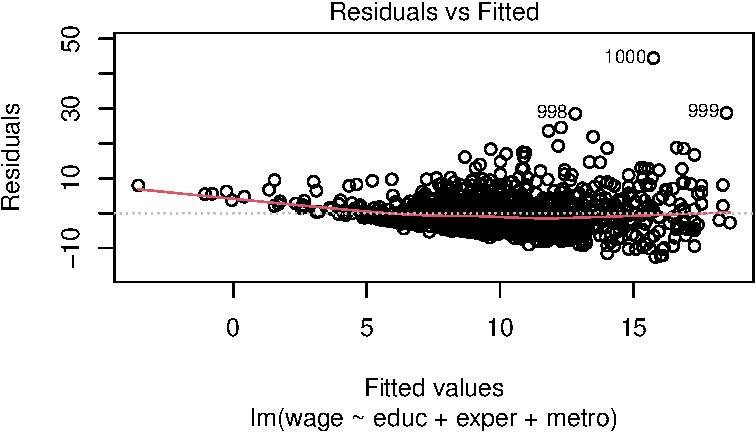
\includegraphics{r-demo-part-3_files/figure-pdf/unnamed-chunk-4-1.pdf}

}

\end{figure}

\begin{Shaded}
\begin{Highlighting}[]
\CommentTok{\# residual QQ plot}
\FunctionTok{plot}\NormalTok{(lm\_fit, }\AttributeTok{which =} \DecValTok{2}\NormalTok{)}
\end{Highlighting}
\end{Shaded}

\begin{figure}[H]

{\centering 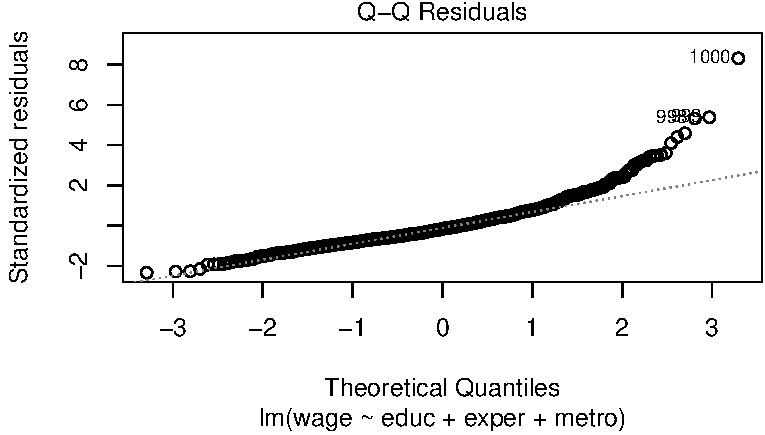
\includegraphics{r-demo-part-3_files/figure-pdf/unnamed-chunk-4-2.pdf}

}

\end{figure}

\begin{Shaded}
\begin{Highlighting}[]
\CommentTok{\# residuals versus leverage (with Cook\textquotesingle{}s distance)}
\FunctionTok{plot}\NormalTok{(lm\_fit, }\AttributeTok{which =} \DecValTok{5}\NormalTok{)}
\end{Highlighting}
\end{Shaded}

\begin{figure}[H]

{\centering 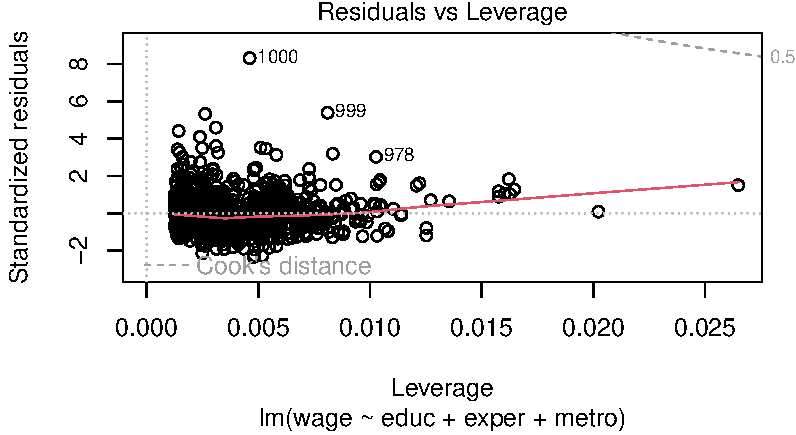
\includegraphics{r-demo-part-3_files/figure-pdf/unnamed-chunk-4-3.pdf}

}

\end{figure}

The residuals versus fitted plot suggests significant
heteroskedasticity, with variance growing as a function of the fitted
value.

\hypertarget{sandwich-standard-errors}{%
\subsection{Sandwich standard errors}\label{sandwich-standard-errors}}

To get standard errors robust to this heteroskedasticity, we can use one
of the robust estimators discussed in
Section~\ref{sec-heteroskedasticity}. Most of the robust standard error
constructions discussed in that section are implemented in the R package
\texttt{sandwich}.

\begin{Shaded}
\begin{Highlighting}[]
\FunctionTok{library}\NormalTok{(sandwich)}
\end{Highlighting}
\end{Shaded}

For example, Huber-White's heteroskedasticity-consistent estimate
\(\widehat{\text{Var}}[\boldsymbol{\widehat \beta}]\) can be obtained
via \texttt{vcovHC}:

\begin{Shaded}
\begin{Highlighting}[]
\NormalTok{HW\_cov }\OtherTok{\textless{}{-}} \FunctionTok{vcovHC}\NormalTok{(lm\_fit)}
\NormalTok{HW\_cov}
\end{Highlighting}
\end{Shaded}

\begin{verbatim}
             (Intercept)          educ         exper         metro
(Intercept)  1.484328645 -0.0967891868 -0.0096871141 -0.1218518012
educ        -0.096789187  0.0070467982  0.0004037764  0.0018334348
exper       -0.009687114  0.0004037764  0.0002517826  0.0008369831
metro       -0.121851801  0.0018334348  0.0008369831  0.1197713348
\end{verbatim}

Compare this to the traditional estimate:

\begin{Shaded}
\begin{Highlighting}[]
\NormalTok{usual\_cov }\OtherTok{\textless{}{-}} \FunctionTok{vcovHC}\NormalTok{(lm\_fit, }\AttributeTok{type =} \StringTok{"const"}\NormalTok{)}
\NormalTok{usual\_cov}
\end{Highlighting}
\end{Shaded}

\begin{verbatim}
             (Intercept)          educ         exper         metro
(Intercept)  1.157049852 -0.0671656102 -0.0070323974 -0.1287058354
educ        -0.067165610  0.0048945781  0.0001924359 -0.0018227782
exper       -0.007032397  0.0001924359  0.0002320022  0.0001471354
metro       -0.128705835 -0.0018227782  0.0001471354  0.1858394060
\end{verbatim}

\begin{Shaded}
\begin{Highlighting}[]
\CommentTok{\# extract the variance estimates from the diagonal}
\FunctionTok{tibble}\NormalTok{(}
  \AttributeTok{variable =} \FunctionTok{rownames}\NormalTok{(usual\_cov),}
  \AttributeTok{usual\_variance =} \FunctionTok{sqrt}\NormalTok{(}\FunctionTok{diag}\NormalTok{(usual\_cov)),}
  \AttributeTok{HW\_variance =} \FunctionTok{sqrt}\NormalTok{(}\FunctionTok{diag}\NormalTok{(HW\_cov))}
\NormalTok{)}
\end{Highlighting}
\end{Shaded}

\begin{verbatim}
# A tibble: 4 x 3
  variable    usual_variance HW_variance
  <chr>                <dbl>       <dbl>
1 (Intercept)         1.08        1.22  
2 educ                0.0700      0.0839
3 exper               0.0152      0.0159
4 metro               0.431       0.346 
\end{verbatim}

Bootstrap standard errors are also implemented in \texttt{sandwich}:

\begin{Shaded}
\begin{Highlighting}[]
\CommentTok{\# pairs bootstrap}
\NormalTok{bootstrap\_cov }\OtherTok{\textless{}{-}} \FunctionTok{vcovBS}\NormalTok{(lm\_fit, }\AttributeTok{type =} \StringTok{"xy"}\NormalTok{)}
\FunctionTok{tibble}\NormalTok{(}
  \AttributeTok{variable =} \FunctionTok{rownames}\NormalTok{(usual\_cov),}
  \AttributeTok{usual\_variance =} \FunctionTok{diag}\NormalTok{(usual\_cov),}
  \AttributeTok{HW\_variance =} \FunctionTok{diag}\NormalTok{(HW\_cov),}
  \AttributeTok{bootstrap\_variance =} \FunctionTok{diag}\NormalTok{(bootstrap\_cov)}
\NormalTok{)}
\end{Highlighting}
\end{Shaded}

\begin{verbatim}
# A tibble: 4 x 4
  variable    usual_variance HW_variance bootstrap_variance
  <chr>                <dbl>       <dbl>              <dbl>
1 (Intercept)       1.16        1.48               1.56    
2 educ              0.00489     0.00705            0.00736 
3 exper             0.000232    0.000252           0.000266
4 metro             0.186       0.120              0.111   
\end{verbatim}

The covariance estimate produced by \texttt{sandwich} can be easily
integrated into linear model inference using the package
\texttt{lmtest}.

\begin{Shaded}
\begin{Highlighting}[]
\FunctionTok{library}\NormalTok{(lmtest)}
\end{Highlighting}
\end{Shaded}

\begin{verbatim}
Loading required package: zoo
\end{verbatim}

\begin{verbatim}

Attaching package: 'zoo'
\end{verbatim}

\begin{verbatim}
The following objects are masked from 'package:base':

    as.Date, as.Date.numeric
\end{verbatim}

\begin{Shaded}
\begin{Highlighting}[]
\CommentTok{\# fit linear model as usual}
\NormalTok{lm\_fit }\OtherTok{\textless{}{-}} \FunctionTok{lm}\NormalTok{(wage }\SpecialCharTok{\textasciitilde{}}\NormalTok{ educ }\SpecialCharTok{+}\NormalTok{ exper }\SpecialCharTok{+}\NormalTok{ metro, }\AttributeTok{data =}\NormalTok{ cps\_data)}

\CommentTok{\# robust t{-}tests for coefficients}
\FunctionTok{coeftest}\NormalTok{(lm\_fit, }\AttributeTok{vcov. =}\NormalTok{ vcovHC)}
\end{Highlighting}
\end{Shaded}

\begin{verbatim}

t test of coefficients:

             Estimate Std. Error t value  Pr(>|t|)    
(Intercept) -9.913984   1.218330 -8.1374 1.197e-15 ***
educ         1.233964   0.083945 14.6996 < 2.2e-16 ***
exper        0.133244   0.015868  8.3972 < 2.2e-16 ***
metro        1.524104   0.346080  4.4039 1.178e-05 ***
---
Signif. codes:  0 '***' 0.001 '**' 0.01 '*' 0.05 '.' 0.1 ' ' 1
\end{verbatim}

\begin{Shaded}
\begin{Highlighting}[]
\CommentTok{\# robust confidence intervals for coefficients}
\FunctionTok{coefci}\NormalTok{(lm\_fit, }\AttributeTok{vcov. =}\NormalTok{ vcovHC)}
\end{Highlighting}
\end{Shaded}

\begin{verbatim}
                  2.5 %     97.5 %
(Intercept) -12.3047729 -7.5231954
educ          1.0692342  1.3986938
exper         0.1021058  0.1643816
metro         0.8449747  2.2032337
\end{verbatim}

\begin{Shaded}
\begin{Highlighting}[]
\CommentTok{\# robust F{-}test}
\NormalTok{lm\_fit\_partial }\OtherTok{\textless{}{-}} \FunctionTok{lm}\NormalTok{(wage }\SpecialCharTok{\textasciitilde{}}\NormalTok{ educ, }\AttributeTok{data =}\NormalTok{ cps\_data) }\CommentTok{\# a partial model}
\FunctionTok{waldtest}\NormalTok{(lm\_fit\_partial, lm\_fit, }\AttributeTok{vcov =}\NormalTok{ vcovHC)}
\end{Highlighting}
\end{Shaded}

\begin{verbatim}
Wald test

Model 1: wage ~ educ
Model 2: wage ~ educ + exper + metro
  Res.Df Df      F    Pr(>F)    
1    998                        
2    996  2 40.252 < 2.2e-16 ***
---
Signif. codes:  0 '***' 0.001 '**' 0.01 '*' 0.05 '.' 0.1 ' ' 1
\end{verbatim}

\hypertarget{bootstrap-confidence-intervals}{%
\subsection{Bootstrap confidence
intervals}\label{bootstrap-confidence-intervals}}

One R package for performing bootstrap inference is \texttt{simpleboot}.
Let's see how to get pairs bootstrap distributions for the coefficient
estimates.

\begin{Shaded}
\begin{Highlighting}[]
\FunctionTok{library}\NormalTok{(simpleboot)}
\end{Highlighting}
\end{Shaded}

\begin{verbatim}
Simple Bootstrap Routines (1.1-8)
\end{verbatim}

\begin{Shaded}
\begin{Highlighting}[]
\NormalTok{boot\_out }\OtherTok{\textless{}{-}} \FunctionTok{lm.boot}\NormalTok{(}
  \AttributeTok{lm.object =}\NormalTok{ lm\_fit, }\CommentTok{\# input the fit object from lm()}
  \AttributeTok{R =} \DecValTok{1000}
\NormalTok{) }\CommentTok{\# R is the number of bootstrap replicates}
\FunctionTok{perc}\NormalTok{(boot\_out) }\CommentTok{\# get the percentile 95\% confidence intervals}
\end{Highlighting}
\end{Shaded}

\begin{verbatim}
      (Intercept)     educ     exper     metro
2.5%   -12.365466 1.075378 0.1034755 0.8985245
97.5%   -7.532934 1.407756 0.1642828 2.1715691
\end{verbatim}

We can extract the resampling distributions for the coefficient
estimates using the \texttt{samples} function:

\begin{Shaded}
\begin{Highlighting}[]
\FunctionTok{samples}\NormalTok{(boot\_out, }\AttributeTok{name =} \StringTok{"coef"}\NormalTok{)[, }\DecValTok{1}\SpecialCharTok{:}\DecValTok{5}\NormalTok{]}
\end{Highlighting}
\end{Shaded}

\begin{verbatim}
                     1           2          3          4          5
(Intercept) -8.5183938 -10.1137042 -9.6244521 -9.6637688 -9.7635183
educ         1.1589410   1.2808242  1.2344501  1.2127978  1.2161110
exper        0.1090993   0.1097745  0.1196861  0.1243353  0.1467017
metro        1.5474578   1.9319631  1.6930226  1.8578930  1.3720004
\end{verbatim}

We can plot these as follows:

\begin{Shaded}
\begin{Highlighting}[]
\NormalTok{boot\_pctiles }\OtherTok{\textless{}{-}}\NormalTok{ boot\_out }\SpecialCharTok{|\textgreater{}}
  \FunctionTok{perc}\NormalTok{() }\SpecialCharTok{|\textgreater{}}
  \FunctionTok{t}\NormalTok{() }\SpecialCharTok{|\textgreater{}}
  \FunctionTok{as.data.frame}\NormalTok{() }\SpecialCharTok{|\textgreater{}}
  \FunctionTok{rownames\_to\_column}\NormalTok{(}\AttributeTok{var =} \StringTok{"var"}\NormalTok{) }\SpecialCharTok{|\textgreater{}}
  \FunctionTok{filter}\NormalTok{(var }\SpecialCharTok{!=} \StringTok{"(Intercept)"}\NormalTok{)}

\FunctionTok{samples}\NormalTok{(boot\_out, }\AttributeTok{name =} \StringTok{"coef"}\NormalTok{) }\SpecialCharTok{|\textgreater{}}
  \FunctionTok{as.data.frame}\NormalTok{() }\SpecialCharTok{|\textgreater{}}
  \FunctionTok{rownames\_to\_column}\NormalTok{(}\AttributeTok{var =} \StringTok{"var"}\NormalTok{) }\SpecialCharTok{|\textgreater{}}
  \FunctionTok{filter}\NormalTok{(var }\SpecialCharTok{!=} \StringTok{"(Intercept)"}\NormalTok{) }\SpecialCharTok{|\textgreater{}}
  \FunctionTok{pivot\_longer}\NormalTok{(}\SpecialCharTok{{-}}\NormalTok{var, }\AttributeTok{names\_to =} \StringTok{"resample"}\NormalTok{, }\AttributeTok{values\_to =} \StringTok{"coefficient"}\NormalTok{) }\SpecialCharTok{|\textgreater{}}
  \FunctionTok{group\_by}\NormalTok{(var) }\SpecialCharTok{|\textgreater{}}
  \FunctionTok{ggplot}\NormalTok{(}\FunctionTok{aes}\NormalTok{(}\AttributeTok{x =}\NormalTok{ coefficient)) }\SpecialCharTok{+}
  \FunctionTok{geom\_histogram}\NormalTok{(}\AttributeTok{bins =} \DecValTok{30}\NormalTok{, }\AttributeTok{colour =} \StringTok{"black"}\NormalTok{) }\SpecialCharTok{+}
  \FunctionTok{geom\_vline}\NormalTok{(}\FunctionTok{aes}\NormalTok{(}\AttributeTok{xintercept =} \StringTok{\textasciigrave{}}\AttributeTok{2.5\%}\StringTok{\textasciigrave{}}\NormalTok{), }\AttributeTok{data =}\NormalTok{ boot\_pctiles, }\AttributeTok{linetype =} \StringTok{"dashed"}\NormalTok{) }\SpecialCharTok{+}
  \FunctionTok{geom\_vline}\NormalTok{(}\FunctionTok{aes}\NormalTok{(}\AttributeTok{xintercept =} \StringTok{\textasciigrave{}}\AttributeTok{97.5\%}\StringTok{\textasciigrave{}}\NormalTok{), }\AttributeTok{data =}\NormalTok{ boot\_pctiles, }\AttributeTok{linetype =} \StringTok{"dashed"}\NormalTok{) }\SpecialCharTok{+}
  \FunctionTok{facet\_wrap}\NormalTok{(}\SpecialCharTok{\textasciitilde{}}\NormalTok{var, }\AttributeTok{scales =} \StringTok{"free"}\NormalTok{)}
\end{Highlighting}
\end{Shaded}

\begin{figure}[H]

{\centering 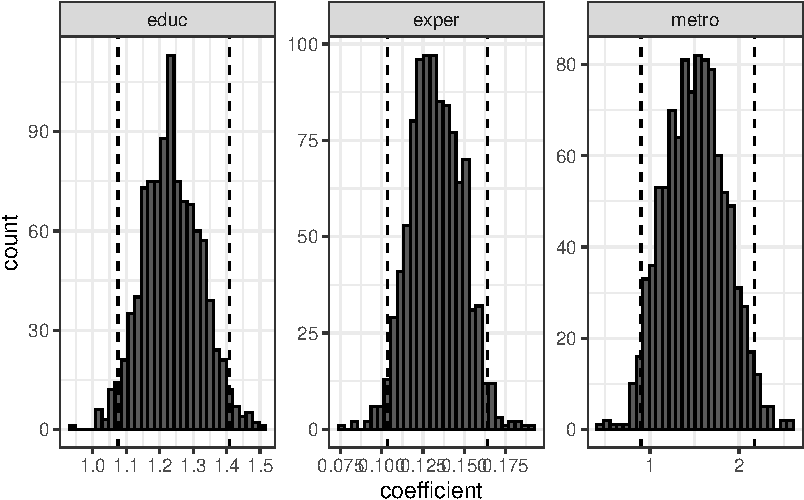
\includegraphics{r-demo-part-3_files/figure-pdf/unnamed-chunk-12-1.pdf}

}

\end{figure}

In this case, the bootstrap sampling distributions look roughly normal.

\hypertarget{group-correlated-errors}{%
\section{Group-correlated errors}\label{group-correlated-errors}}

Credit for this data example:
\url{https://www.r-bloggers.com/2021/05/clustered-standard-errors-with-r/}.

Let's consider the \texttt{nslwork} data from the \texttt{webuse}
package:

\begin{Shaded}
\begin{Highlighting}[]
\FunctionTok{library}\NormalTok{(webuse)}
\NormalTok{nlswork\_orig }\OtherTok{\textless{}{-}} \FunctionTok{webuse}\NormalTok{(}\StringTok{"nlswork"}\NormalTok{)}
\NormalTok{nlswork }\OtherTok{\textless{}{-}}\NormalTok{ nlswork\_orig }\SpecialCharTok{|\textgreater{}}
  \FunctionTok{filter}\NormalTok{(idcode }\SpecialCharTok{\textless{}=} \DecValTok{100}\NormalTok{) }\SpecialCharTok{|\textgreater{}}
  \FunctionTok{select}\NormalTok{(idcode, year, ln\_wage, age, tenure, union) }\SpecialCharTok{|\textgreater{}}
  \FunctionTok{na.omit}\NormalTok{() }\SpecialCharTok{|\textgreater{}}
  \FunctionTok{mutate}\NormalTok{(}
    \AttributeTok{union =} \FunctionTok{as.integer}\NormalTok{(union),}
    \AttributeTok{idcode =} \FunctionTok{as.factor}\NormalTok{(idcode)}
\NormalTok{  )}
\NormalTok{nlswork}
\end{Highlighting}
\end{Shaded}

\begin{verbatim}
# A tibble: 386 x 6
   idcode  year ln_wage   age tenure union
   <fct>  <dbl>   <dbl> <dbl>  <dbl> <int>
 1 1         72    1.59    20  0.917     1
 2 1         77    1.78    25  1.5       0
 3 1         80    2.55    28  1.83      1
 4 1         83    2.42    31  0.667     1
 5 1         85    2.61    33  1.92      1
 6 1         87    2.54    35  3.92      1
 7 1         88    2.46    37  5.33      1
 8 2         71    1.36    19  0.25      0
 9 2         77    1.73    25  2.67      1
10 2         78    1.69    26  3.67      1
# i 376 more rows
\end{verbatim}

The data comes from the US National Longitudinal Survey (NLS) and
contains information about more than 4,000 young working women. We're
interested in the relationship between wage (here as log-scaled
GNP-adjusted wage) \texttt{ln\_wage} and survey participant's current
age, job tenure in years, and union membership as independent variables.
It's a longitudinal survey, so subjects were asked repeatedly between
1968 and 1988, and each subject is identified by a unique idcode
\texttt{idcode}. Here we restrict attention to the first 100 subjects
and remove any rows with missing data.

Let's start by fitting a linear regression of the log wage on
\texttt{age}, \texttt{tenure}, \texttt{union}, and the interaction
between \texttt{tenure} and \texttt{union}:

\begin{Shaded}
\begin{Highlighting}[]
\NormalTok{lm\_fit }\OtherTok{\textless{}{-}} \FunctionTok{lm}\NormalTok{(ln\_wage }\SpecialCharTok{\textasciitilde{}}\NormalTok{ age }\SpecialCharTok{+}\NormalTok{ tenure }\SpecialCharTok{+}\NormalTok{ union }\SpecialCharTok{+}\NormalTok{ tenure}\SpecialCharTok{:}\NormalTok{union, }\AttributeTok{data =}\NormalTok{ nlswork)}
\FunctionTok{summary}\NormalTok{(lm\_fit)}
\end{Highlighting}
\end{Shaded}

\begin{verbatim}

Call:
lm(formula = ln_wage ~ age + tenure + union + tenure:union, data = nlswork)

Residuals:
     Min       1Q   Median       3Q      Max 
-1.42570 -0.28330  0.01694  0.27303  1.65052 

Coefficients:
              Estimate Std. Error t value Pr(>|t|)    
(Intercept)   1.379103   0.099658  13.838  < 2e-16 ***
age           0.013553   0.003388   4.000 7.60e-05 ***
tenure        0.022175   0.008051   2.754  0.00617 ** 
union         0.309936   0.070344   4.406 1.37e-05 ***
tenure:union -0.009629   0.012049  -0.799  0.42473    
---
Signif. codes:  0 '***' 0.001 '**' 0.01 '*' 0.05 '.' 0.1 ' ' 1

Residual standard error: 0.4099 on 381 degrees of freedom
Multiple R-squared:  0.1811,    Adjusted R-squared:  0.1725 
F-statistic: 21.07 on 4 and 381 DF,  p-value: 1.047e-15
\end{verbatim}

Let's plot the residuals against the individuals:

\begin{Shaded}
\begin{Highlighting}[]
\NormalTok{nlswork }\SpecialCharTok{|\textgreater{}}
  \FunctionTok{mutate}\NormalTok{(}\AttributeTok{resid =}\NormalTok{ lm\_fit}\SpecialCharTok{$}\NormalTok{residuals) }\SpecialCharTok{|\textgreater{}}
  \FunctionTok{ggplot}\NormalTok{(}\FunctionTok{aes}\NormalTok{(}\AttributeTok{x =}\NormalTok{ idcode, }\AttributeTok{y =}\NormalTok{ resid)) }\SpecialCharTok{+}
  \FunctionTok{geom\_boxplot}\NormalTok{() }\SpecialCharTok{+}
  \FunctionTok{labs}\NormalTok{(}
    \AttributeTok{x =} \StringTok{"Subject"}\NormalTok{,}
    \AttributeTok{y =} \StringTok{"Residual"}
\NormalTok{  ) }\SpecialCharTok{+}
  \FunctionTok{theme}\NormalTok{(}\AttributeTok{axis.text.x =} \FunctionTok{element\_blank}\NormalTok{())}
\end{Highlighting}
\end{Shaded}

\begin{figure}[H]

{\centering 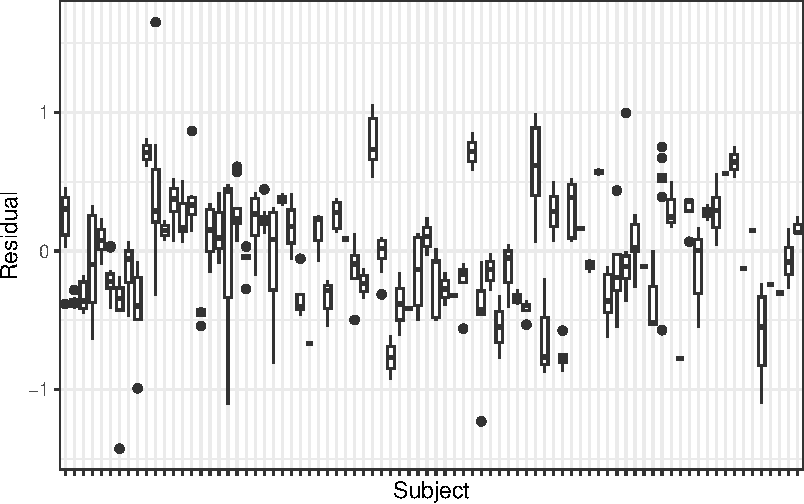
\includegraphics{r-demo-part-3_files/figure-pdf/unnamed-chunk-15-1.pdf}

}

\end{figure}

Clearly, there is dependency among the residuals within subjects.
Therefore, we have either model bias, or correlated errors, or both. To
help assess whether we have model bias or not, we must check whether the
variables of interest are correlated with the grouping variable
\texttt{idcode}. We can check this with a plot, e.g., for the
\texttt{tenure} variable:

\begin{Shaded}
\begin{Highlighting}[]
\NormalTok{nlswork }\SpecialCharTok{|\textgreater{}}
  \FunctionTok{ggplot}\NormalTok{(}\FunctionTok{aes}\NormalTok{(}\AttributeTok{x =}\NormalTok{ idcode, }\AttributeTok{y =}\NormalTok{ tenure)) }\SpecialCharTok{+}
  \FunctionTok{geom\_boxplot}\NormalTok{() }\SpecialCharTok{+}
  \FunctionTok{labs}\NormalTok{(}
    \AttributeTok{x =} \StringTok{"Subject"}\NormalTok{,}
    \AttributeTok{y =} \StringTok{"Tenure"}
\NormalTok{  ) }\SpecialCharTok{+}
  \FunctionTok{theme}\NormalTok{(}\AttributeTok{axis.text.x =} \FunctionTok{element\_blank}\NormalTok{())}
\end{Highlighting}
\end{Shaded}

\begin{figure}[H]

{\centering 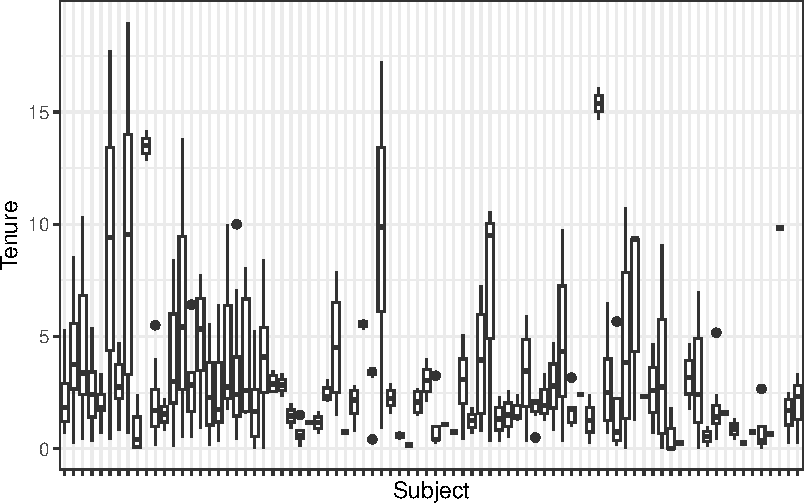
\includegraphics{r-demo-part-3_files/figure-pdf/unnamed-chunk-16-1.pdf}

}

\end{figure}

Again, there seems to be nontrivial association between \texttt{tenure}
and \texttt{idcode}. We can check this more formally with an ANOVA test:

\begin{Shaded}
\begin{Highlighting}[]
\FunctionTok{summary}\NormalTok{(}\FunctionTok{aov}\NormalTok{(tenure }\SpecialCharTok{\textasciitilde{}}\NormalTok{ idcode, }\AttributeTok{data =}\NormalTok{ nlswork))}
\end{Highlighting}
\end{Shaded}

\begin{verbatim}
             Df Sum Sq Mean Sq F value   Pr(>F)    
idcode       81   2529  31.220   3.558 8.83e-16 ***
Residuals   304   2668   8.775                     
---
Signif. codes:  0 '***' 0.001 '**' 0.01 '*' 0.05 '.' 0.1 ' ' 1
\end{verbatim}

So, in this case, we do have model bias on our hands. We can address
this using fixed effects for each subject.

\begin{Shaded}
\begin{Highlighting}[]
\NormalTok{lm\_fit\_FE }\OtherTok{\textless{}{-}} \FunctionTok{lm}\NormalTok{(ln\_wage }\SpecialCharTok{\textasciitilde{}}\NormalTok{ age }\SpecialCharTok{+}\NormalTok{ tenure }\SpecialCharTok{+}\NormalTok{ union }\SpecialCharTok{+}\NormalTok{ tenure}\SpecialCharTok{:}\NormalTok{union }\SpecialCharTok{+}\NormalTok{ idcode, }\AttributeTok{data =}\NormalTok{ nlswork)}
\NormalTok{lm\_fit\_FE }\SpecialCharTok{|\textgreater{}}
  \FunctionTok{summary}\NormalTok{() }\SpecialCharTok{|\textgreater{}}
  \FunctionTok{coef}\NormalTok{() }\SpecialCharTok{|\textgreater{}}
  \FunctionTok{as.data.frame}\NormalTok{() }\SpecialCharTok{|\textgreater{}}
  \FunctionTok{rownames\_to\_column}\NormalTok{(}\AttributeTok{var =} \StringTok{"var"}\NormalTok{) }\SpecialCharTok{|\textgreater{}}
  \FunctionTok{filter}\NormalTok{(}\SpecialCharTok{!}\FunctionTok{grepl}\NormalTok{(}\StringTok{"idcode"}\NormalTok{, var)) }\SpecialCharTok{|\textgreater{}} \CommentTok{\# remove coefficients for fixed effects}
  \FunctionTok{column\_to\_rownames}\NormalTok{(}\AttributeTok{var =} \StringTok{"var"}\NormalTok{)}
\end{Highlighting}
\end{Shaded}

\begin{verbatim}
                Estimate  Std. Error   t value     Pr(>|t|)
(Intercept)  1.882478232 0.131411504 14.325064 8.022367e-36
age          0.005630809 0.003109803  1.810664 7.119315e-02
tenure       0.020756426 0.006964417  2.980353 3.114742e-03
union        0.174619394 0.060646038  2.879321 4.272027e-03
tenure:union 0.014974113 0.009548509  1.568215 1.178851e-01
\end{verbatim}

Note the changes in the standard errors and p-values. Sometimes, we may
have remaining correlation among residuals even after adding cluster
fixed effects. Therefore, it is common practice to compute clustered
(i.e., Liang-Zeger) standard errors in conjunction with cluster fixed
effects. We can get clustered standard errors via the \texttt{vcovCL}
function from \texttt{sandwich}:

\begin{Shaded}
\begin{Highlighting}[]
\NormalTok{LZ\_cov }\OtherTok{\textless{}{-}} \FunctionTok{vcovCL}\NormalTok{(lm\_fit\_FE, }\AttributeTok{cluster =}\NormalTok{ nlswork}\SpecialCharTok{$}\NormalTok{idcode)}
\FunctionTok{coeftest}\NormalTok{(lm\_fit\_FE, }\AttributeTok{vcov. =}\NormalTok{ LZ\_cov)[, ] }\SpecialCharTok{|\textgreater{}}
  \FunctionTok{as.data.frame}\NormalTok{() }\SpecialCharTok{|\textgreater{}}
  \FunctionTok{rownames\_to\_column}\NormalTok{(}\AttributeTok{var =} \StringTok{"var"}\NormalTok{) }\SpecialCharTok{|\textgreater{}}
  \FunctionTok{filter}\NormalTok{(}\SpecialCharTok{!}\FunctionTok{grepl}\NormalTok{(}\StringTok{"idcode"}\NormalTok{, var)) }\SpecialCharTok{|\textgreater{}} \CommentTok{\# remove coefficients for fixed effects}
  \FunctionTok{column\_to\_rownames}\NormalTok{(}\AttributeTok{var =} \StringTok{"var"}\NormalTok{)}
\end{Highlighting}
\end{Shaded}

\begin{verbatim}
                Estimate  Std. Error    t value     Pr(>|t|)
(Intercept)  1.882478232 0.157611390 11.9437956 3.667970e-27
age          0.005630809 0.006339777  0.8881715 3.751601e-01
tenure       0.020756426 0.011149190  1.8616981 6.362342e-02
union        0.174619394 0.101970509  1.7124500 8.784708e-02
tenure:union 0.014974113 0.009646023  1.5523613 1.216301e-01
\end{verbatim}

Again, note the changes in the standard errors and p-values.

\hypertarget{autocorrelated-errors}{%
\section{Autocorrelated errors}\label{autocorrelated-errors}}

Let's take a look at the \texttt{EuStockMarkets} data built into R,
containing the daily closing prices of major European stock indices:
Germany DAX (Ibis), Switzerland SMI, France CAC, and UK FTSE. Let's
regress \texttt{DAX} on \texttt{FTSE} and take a look at the residuals:

\begin{Shaded}
\begin{Highlighting}[]
\NormalTok{lm\_fit }\OtherTok{\textless{}{-}} \FunctionTok{lm}\NormalTok{(DAX }\SpecialCharTok{\textasciitilde{}}\NormalTok{ FTSE, }\AttributeTok{data =}\NormalTok{ EuStockMarkets)}
\FunctionTok{summary}\NormalTok{(lm\_fit)}
\end{Highlighting}
\end{Shaded}

\begin{verbatim}

Call:
lm(formula = DAX ~ FTSE, data = EuStockMarkets)

Residuals:
    Min      1Q  Median      3Q     Max 
-408.43 -172.53  -45.71  137.68  989.96 

Coefficients:
              Estimate Std. Error t value Pr(>|t|)    
(Intercept) -1.331e+03  2.109e+01  -63.12   <2e-16 ***
FTSE         1.083e+00  5.705e-03  189.84   <2e-16 ***
---
Signif. codes:  0 '***' 0.001 '**' 0.01 '*' 0.05 '.' 0.1 ' ' 1

Residual standard error: 240.3 on 1858 degrees of freedom
Multiple R-squared:  0.951, Adjusted R-squared:  0.9509 
F-statistic: 3.604e+04 on 1 and 1858 DF,  p-value: < 2.2e-16
\end{verbatim}

We find an extremely significant association between the two stock
indices. But let's examine the residuals for autocorrelation:

\begin{Shaded}
\begin{Highlighting}[]
\NormalTok{EuStockMarkets }\SpecialCharTok{|\textgreater{}}
  \FunctionTok{as.data.frame}\NormalTok{() }\SpecialCharTok{|\textgreater{}}
  \FunctionTok{mutate}\NormalTok{(}
    \AttributeTok{date =} \FunctionTok{row\_number}\NormalTok{(),}
    \AttributeTok{resid =}\NormalTok{ lm\_fit}\SpecialCharTok{$}\NormalTok{residuals}
\NormalTok{  ) }\SpecialCharTok{|\textgreater{}}
  \FunctionTok{ggplot}\NormalTok{(}\FunctionTok{aes}\NormalTok{(}\AttributeTok{x =}\NormalTok{ date, }\AttributeTok{y =}\NormalTok{ resid)) }\SpecialCharTok{+}
  \FunctionTok{geom\_line}\NormalTok{() }\SpecialCharTok{+}
  \FunctionTok{labs}\NormalTok{(}
    \AttributeTok{x =} \StringTok{"Day"}\NormalTok{,}
    \AttributeTok{y =} \StringTok{"Residual"}
\NormalTok{  )}
\end{Highlighting}
\end{Shaded}

\begin{figure}[H]

{\centering 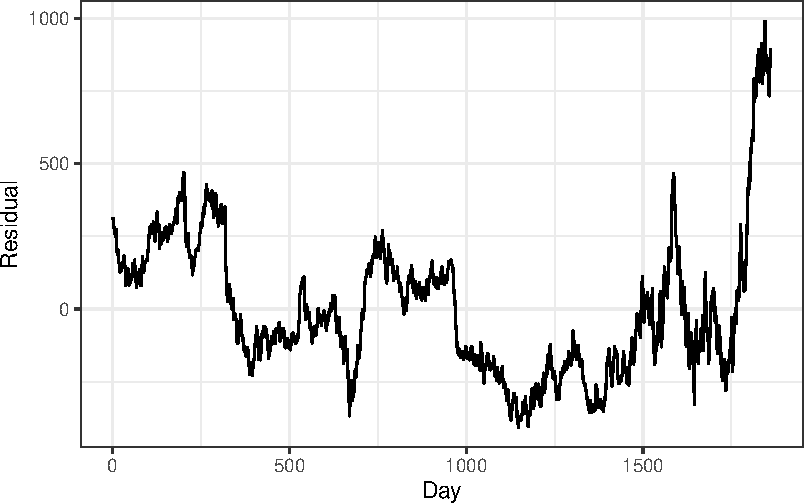
\includegraphics{r-demo-part-3_files/figure-pdf/unnamed-chunk-21-1.pdf}

}

\end{figure}

There is clearly some autocorrelation in the residuals. Let's quantify
it using the autocorrelation function (\texttt{acf()} in R):

\begin{Shaded}
\begin{Highlighting}[]
\FunctionTok{acf}\NormalTok{(lm\_fit}\SpecialCharTok{$}\NormalTok{residuals, }\AttributeTok{lag.max =} \DecValTok{1000}\NormalTok{)}
\end{Highlighting}
\end{Shaded}

\begin{figure}[H]

{\centering 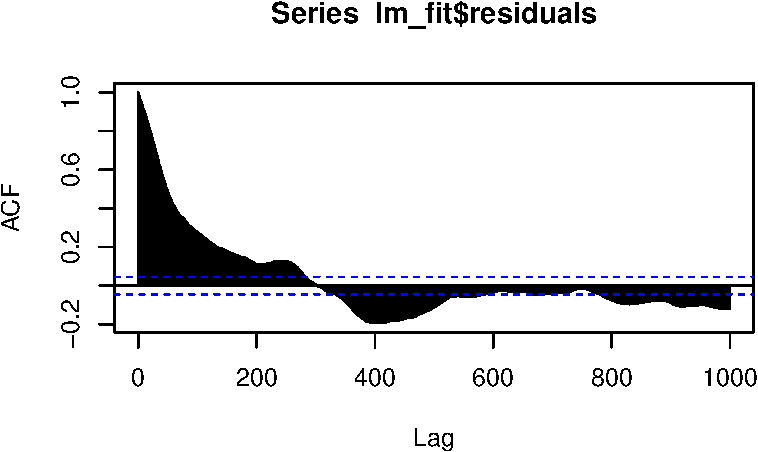
\includegraphics{r-demo-part-3_files/figure-pdf/unnamed-chunk-22-1.pdf}

}

\end{figure}

We see that the autocorrelation gets into a reasonably low range around
lag 200. We can then construct Newey-West standard errors based on this
lag:

\begin{Shaded}
\begin{Highlighting}[]
\NormalTok{NW\_cov }\OtherTok{\textless{}{-}} \FunctionTok{NeweyWest}\NormalTok{(lm\_fit)}
\FunctionTok{coeftest}\NormalTok{(lm\_fit, }\AttributeTok{vcov. =}\NormalTok{ NW\_cov)}
\end{Highlighting}
\end{Shaded}

\begin{verbatim}

t test of coefficients:

              Estimate Std. Error t value Pr(>|t|)
(Intercept) -1331.2374  4398.3722 -0.3027   0.7622
FTSE            1.0831     1.4645  0.7396   0.4597
\end{verbatim}

We see that the p-value for the association goes from \texttt{2e-16} to
\texttt{0.46}, after accounting for autocorrelation.

\hypertarget{outliers}{%
\section{Outliers}\label{outliers}}

Let's take a look at the crime data from HW2:

\begin{Shaded}
\begin{Highlighting}[]
\CommentTok{\# read crime data}
\NormalTok{crime\_data }\OtherTok{\textless{}{-}} \FunctionTok{read\_tsv}\NormalTok{(}\StringTok{"data/Statewide\_crime.dat"}\NormalTok{)}
\end{Highlighting}
\end{Shaded}

\begin{verbatim}
Rows: 51 Columns: 6
-- Column specification --------------------------------------------------------
Delimiter: "\t"
chr (1): STATE
dbl (5): Violent, Murder, Metro, HighSchool, Poverty

i Use `spec()` to retrieve the full column specification for this data.
i Specify the column types or set `show_col_types = FALSE` to quiet this message.
\end{verbatim}

\begin{Shaded}
\begin{Highlighting}[]
\CommentTok{\# read and transform population data}
\NormalTok{population\_data }\OtherTok{\textless{}{-}} \FunctionTok{read\_csv}\NormalTok{(}\StringTok{"data/state{-}populations.csv"}\NormalTok{)}
\end{Highlighting}
\end{Shaded}

\begin{verbatim}
Rows: 52 Columns: 9
-- Column specification --------------------------------------------------------
Delimiter: ","
chr (1): State
dbl (8): rank, Pop, Growth, Pop2018, Pop2010, growthSince2010, Percent, density

i Use `spec()` to retrieve the full column specification for this data.
i Specify the column types or set `show_col_types = FALSE` to quiet this message.
\end{verbatim}

\begin{Shaded}
\begin{Highlighting}[]
\NormalTok{population\_data }\OtherTok{\textless{}{-}}\NormalTok{ population\_data }\SpecialCharTok{|\textgreater{}}
  \FunctionTok{filter}\NormalTok{(State }\SpecialCharTok{!=} \StringTok{"Puerto Rico"}\NormalTok{) }\SpecialCharTok{|\textgreater{}}
  \FunctionTok{select}\NormalTok{(State, Pop) }\SpecialCharTok{|\textgreater{}}
  \FunctionTok{rename}\NormalTok{(}\AttributeTok{state\_name =}\NormalTok{ State, }\AttributeTok{state\_pop =}\NormalTok{ Pop)}

\CommentTok{\# collate state abbreviations}
\NormalTok{state\_abbreviations }\OtherTok{\textless{}{-}} \FunctionTok{tibble}\NormalTok{(}
  \AttributeTok{state\_name =}\NormalTok{ state.name,}
  \AttributeTok{state\_abbrev =}\NormalTok{ state.abb}
\NormalTok{) }\SpecialCharTok{|\textgreater{}}
  \FunctionTok{add\_row}\NormalTok{(}\AttributeTok{state\_name =} \StringTok{"District of Columbia"}\NormalTok{, }\AttributeTok{state\_abbrev =} \StringTok{"DC"}\NormalTok{)}

\CommentTok{\# add CrimeRate to crime\_data}
\NormalTok{crime\_data }\OtherTok{\textless{}{-}}\NormalTok{ crime\_data }\SpecialCharTok{|\textgreater{}}
  \FunctionTok{mutate}\NormalTok{(}\AttributeTok{STATE =} \FunctionTok{ifelse}\NormalTok{(STATE }\SpecialCharTok{==} \StringTok{"IO"}\NormalTok{, }\StringTok{"IA"}\NormalTok{, STATE)) }\SpecialCharTok{|\textgreater{}}
  \FunctionTok{rename}\NormalTok{(}\AttributeTok{state\_abbrev =}\NormalTok{ STATE) }\SpecialCharTok{|\textgreater{}}
  \FunctionTok{left\_join}\NormalTok{(state\_abbreviations, }\AttributeTok{by =} \StringTok{"state\_abbrev"}\NormalTok{) }\SpecialCharTok{|\textgreater{}}
  \FunctionTok{left\_join}\NormalTok{(population\_data, }\AttributeTok{by =} \StringTok{"state\_name"}\NormalTok{) }\SpecialCharTok{|\textgreater{}}
  \FunctionTok{mutate}\NormalTok{(}\AttributeTok{CrimeRate =}\NormalTok{ Violent }\SpecialCharTok{/}\NormalTok{ state\_pop) }\SpecialCharTok{|\textgreater{}}
  \FunctionTok{select}\NormalTok{(state\_abbrev, CrimeRate, Metro, HighSchool, Poverty)}

\NormalTok{crime\_data}
\end{Highlighting}
\end{Shaded}

\begin{verbatim}
# A tibble: 51 x 5
   state_abbrev CrimeRate Metro HighSchool Poverty
   <chr>            <dbl> <dbl>      <dbl>   <dbl>
 1 AK           0.000819   65.6       90.2     8  
 2 AL           0.0000871  55.4       82.4    13.7
 3 AR           0.000150   52.5       79.2    12.1
 4 AZ           0.0000682  88.2       84.4    11.9
 5 CA           0.0000146  94.4       81.3    10.5
 6 CO           0.0000585  84.5       88.3     7.3
 7 CT           0.0000867  87.7       88.8     6.4
 8 DE           0.000664   80.1       86.5     5.8
 9 FL           0.0000333  89.3       85.9     9.7
10 GA           0.0000419  71.6       85.2    10.8
# i 41 more rows
\end{verbatim}

Let's fit the linear regression:

\begin{Shaded}
\begin{Highlighting}[]
\CommentTok{\# note: we make the state abbreviations row names for better diagnostic plots}
\NormalTok{lm\_fit }\OtherTok{\textless{}{-}} \FunctionTok{lm}\NormalTok{(CrimeRate }\SpecialCharTok{\textasciitilde{}}\NormalTok{ Metro }\SpecialCharTok{+}\NormalTok{ HighSchool }\SpecialCharTok{+}\NormalTok{ Poverty, }\AttributeTok{data =}\NormalTok{ crime\_data }\SpecialCharTok{|\textgreater{}} \FunctionTok{column\_to\_rownames}\NormalTok{(}\AttributeTok{var =} \StringTok{"state\_abbrev"}\NormalTok{))}
\end{Highlighting}
\end{Shaded}

We can get the standard linear regression diagnostic plots as follows:

\begin{Shaded}
\begin{Highlighting}[]
\CommentTok{\# residuals versus fitted}
\FunctionTok{plot}\NormalTok{(lm\_fit, }\AttributeTok{which =} \DecValTok{1}\NormalTok{)}
\end{Highlighting}
\end{Shaded}

\begin{figure}[H]

{\centering 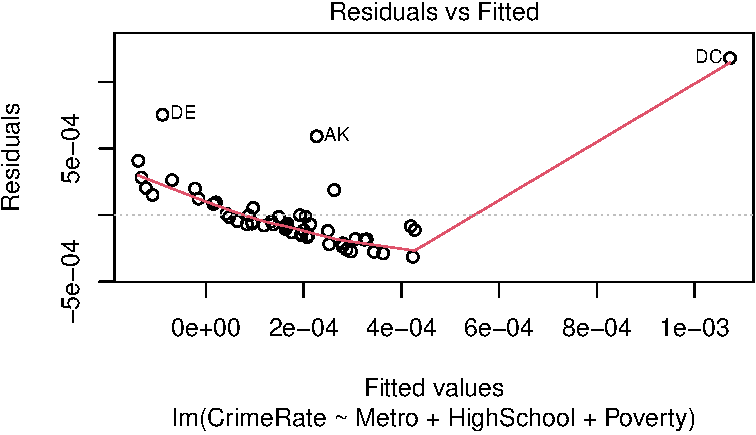
\includegraphics{r-demo-part-3_files/figure-pdf/unnamed-chunk-26-1.pdf}

}

\end{figure}

\begin{Shaded}
\begin{Highlighting}[]
\CommentTok{\# residual QQ plot}
\FunctionTok{plot}\NormalTok{(lm\_fit, }\AttributeTok{which =} \DecValTok{2}\NormalTok{)}
\end{Highlighting}
\end{Shaded}

\begin{figure}[H]

{\centering 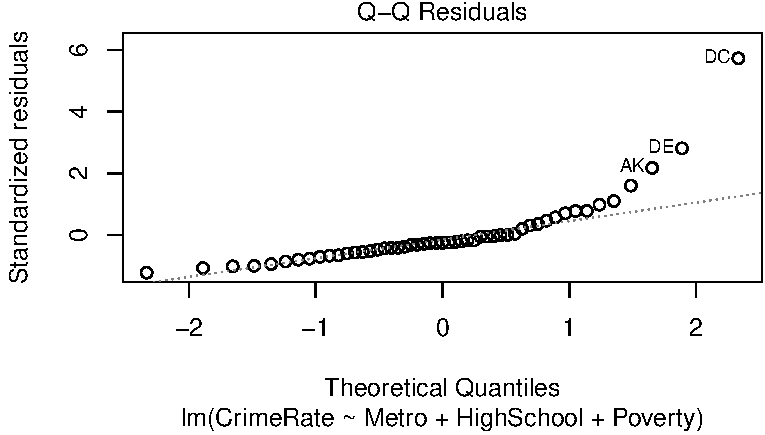
\includegraphics{r-demo-part-3_files/figure-pdf/unnamed-chunk-26-2.pdf}

}

\end{figure}

\begin{Shaded}
\begin{Highlighting}[]
\CommentTok{\# residuals versus leverage (with Cook\textquotesingle{}s distance)}
\FunctionTok{plot}\NormalTok{(lm\_fit, }\AttributeTok{which =} \DecValTok{5}\NormalTok{)}
\end{Highlighting}
\end{Shaded}

\begin{figure}[H]

{\centering 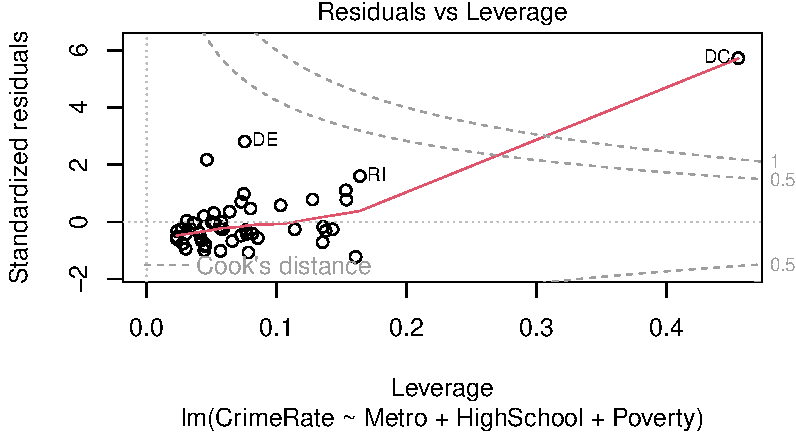
\includegraphics{r-demo-part-3_files/figure-pdf/unnamed-chunk-26-3.pdf}

}

\end{figure}

The information underlying these diagnostic plots can be extracted as
follows:

\begin{Shaded}
\begin{Highlighting}[]
\FunctionTok{tibble}\NormalTok{(}
  \AttributeTok{state =}\NormalTok{ crime\_data}\SpecialCharTok{$}\NormalTok{state\_abbrev,}
  \AttributeTok{std\_residual =} \FunctionTok{rstandard}\NormalTok{(lm\_fit),}
  \AttributeTok{fitted\_value =} \FunctionTok{fitted.values}\NormalTok{(lm\_fit),}
  \AttributeTok{leverage =} \FunctionTok{hatvalues}\NormalTok{(lm\_fit),}
  \AttributeTok{cooks\_dist =} \FunctionTok{cooks.distance}\NormalTok{(lm\_fit)}
\NormalTok{)}
\end{Highlighting}
\end{Shaded}

\begin{verbatim}
# A tibble: 51 x 5
   state std_residual fitted_value leverage cooks_dist
   <chr>        <dbl>        <dbl>    <dbl>      <dbl>
 1 AK           2.17     0.000227    0.0463   0.0574  
 2 AL          -0.422    0.000200    0.0769   0.00371 
 3 AR           1.10    -0.000132    0.153    0.0547  
 4 AZ          -1.02     0.000344    0.0568   0.0156  
 5 CA          -0.264    0.0000839   0.114    0.00224 
 6 CO          -0.383    0.000163    0.0405   0.00155 
 7 CT          -0.175    0.000134    0.0561   0.000456
 8 DE           2.81    -0.0000888   0.0754   0.161   
 9 FL          -0.804    0.000252    0.0452   0.00764 
10 GA          -0.599    0.000207    0.0232   0.00213 
# i 41 more rows
\end{verbatim}

Clearly, DC is an outlier. We can either run a robust estimation
procedure or redo the analysis without DC. Let's try both. First, we try
robust regression using \texttt{rlm()} from the \texttt{MASS} package:

\begin{Shaded}
\begin{Highlighting}[]
\NormalTok{rlm\_fit }\OtherTok{\textless{}{-}}\NormalTok{ MASS}\SpecialCharTok{::}\FunctionTok{rlm}\NormalTok{(CrimeRate }\SpecialCharTok{\textasciitilde{}}\NormalTok{ Metro }\SpecialCharTok{+}\NormalTok{ HighSchool }\SpecialCharTok{+}\NormalTok{ Poverty, }\AttributeTok{data =}\NormalTok{ crime\_data)}
\FunctionTok{summary}\NormalTok{(rlm\_fit)}
\end{Highlighting}
\end{Shaded}

\begin{verbatim}

Call: rlm(formula = CrimeRate ~ Metro + HighSchool + Poverty, data = crime_data)
Residuals:
       Min         1Q     Median         3Q        Max 
-8.297e-05 -3.787e-05 -2.249e-05  4.407e-05  2.063e-03 

Coefficients:
            Value   Std. Error t value
(Intercept) -0.0009  0.0004    -2.2562
Metro        0.0000  0.0000    -1.2963
HighSchool   0.0000  0.0000     2.6506
Poverty      0.0000  0.0000     2.7546

Residual standard error: 6.048e-05 on 47 degrees of freedom
\end{verbatim}

For some reason, the p-values are not computed automatically. We can
compute them ourselves instead:

\begin{Shaded}
\begin{Highlighting}[]
\FunctionTok{summary}\NormalTok{(rlm\_fit)}\SpecialCharTok{$}\NormalTok{coef }\SpecialCharTok{|\textgreater{}}
  \FunctionTok{as.data.frame}\NormalTok{() }\SpecialCharTok{|\textgreater{}}
  \FunctionTok{rename}\NormalTok{(}\AttributeTok{Estimate =}\NormalTok{ Value) }\SpecialCharTok{|\textgreater{}}
  \FunctionTok{mutate}\NormalTok{(}\StringTok{\textasciigrave{}}\AttributeTok{p value}\StringTok{\textasciigrave{}} \OtherTok{=} \DecValTok{2} \SpecialCharTok{*} \FunctionTok{dnorm}\NormalTok{(}\SpecialCharTok{{-}}\FunctionTok{abs}\NormalTok{(}\StringTok{\textasciigrave{}}\AttributeTok{t value}\StringTok{\textasciigrave{}}\NormalTok{)))}
\end{Highlighting}
\end{Shaded}

\begin{verbatim}
                 Estimate   Std. Error   t value    p value
(Intercept) -8.538466e-04 3.784466e-04 -2.256188 0.06260042
Metro       -8.639252e-07 6.664623e-07 -1.296285 0.34439400
HighSchool   1.037849e-05 3.915573e-06  2.650568 0.02378865
Poverty      1.252839e-05 4.548172e-06  2.754600 0.01795833
\end{verbatim}

To see the robust estimation action visually, let's consider a
univariate example:

\begin{Shaded}
\begin{Highlighting}[]
\NormalTok{lm\_fit }\OtherTok{\textless{}{-}} \FunctionTok{lm}\NormalTok{(CrimeRate }\SpecialCharTok{\textasciitilde{}}\NormalTok{ Metro, }\AttributeTok{data =}\NormalTok{ crime\_data)}
\NormalTok{rlm\_fit }\OtherTok{\textless{}{-}}\NormalTok{ MASS}\SpecialCharTok{::}\FunctionTok{rlm}\NormalTok{(CrimeRate }\SpecialCharTok{\textasciitilde{}}\NormalTok{ Metro, }\AttributeTok{data =}\NormalTok{ crime\_data)}

\CommentTok{\# collate the fits into a tibble}
\NormalTok{line\_fits }\OtherTok{\textless{}{-}} \FunctionTok{tibble}\NormalTok{(}
  \AttributeTok{method =} \FunctionTok{c}\NormalTok{(}\StringTok{"Usual"}\NormalTok{, }\StringTok{"Robust"}\NormalTok{),}
  \AttributeTok{intercept =} \FunctionTok{c}\NormalTok{(}
    \FunctionTok{coef}\NormalTok{(lm\_fit)[}\StringTok{"(Intercept)"}\NormalTok{],}
    \FunctionTok{coef}\NormalTok{(rlm\_fit)[}\StringTok{"(Intercept)"}\NormalTok{]}
\NormalTok{  ),}
  \AttributeTok{slope =} \FunctionTok{c}\NormalTok{(}
    \FunctionTok{coef}\NormalTok{(lm\_fit)[}\StringTok{"Metro"}\NormalTok{],}
    \FunctionTok{coef}\NormalTok{(rlm\_fit)[}\StringTok{"Metro"}\NormalTok{]}
\NormalTok{  )}
\NormalTok{)}
\end{Highlighting}
\end{Shaded}

\begin{Shaded}
\begin{Highlighting}[]
\CommentTok{\# usual and robust univariate fits}
\CommentTok{\# plot the fits}
\NormalTok{crime\_data }\SpecialCharTok{|\textgreater{}}
  \FunctionTok{ggplot}\NormalTok{() }\SpecialCharTok{+}
  \FunctionTok{geom\_point}\NormalTok{(}\FunctionTok{aes}\NormalTok{(}\AttributeTok{x =}\NormalTok{ Metro, }\AttributeTok{y =}\NormalTok{ CrimeRate)) }\SpecialCharTok{+}
  \FunctionTok{geom\_abline}\NormalTok{(}\FunctionTok{aes}\NormalTok{(}\AttributeTok{intercept =}\NormalTok{ intercept, }\AttributeTok{slope =}\NormalTok{ slope, }\AttributeTok{colour =}\NormalTok{ method), }\AttributeTok{data =}\NormalTok{ line\_fits)}
\end{Highlighting}
\end{Shaded}

\begin{figure}[H]

{\centering 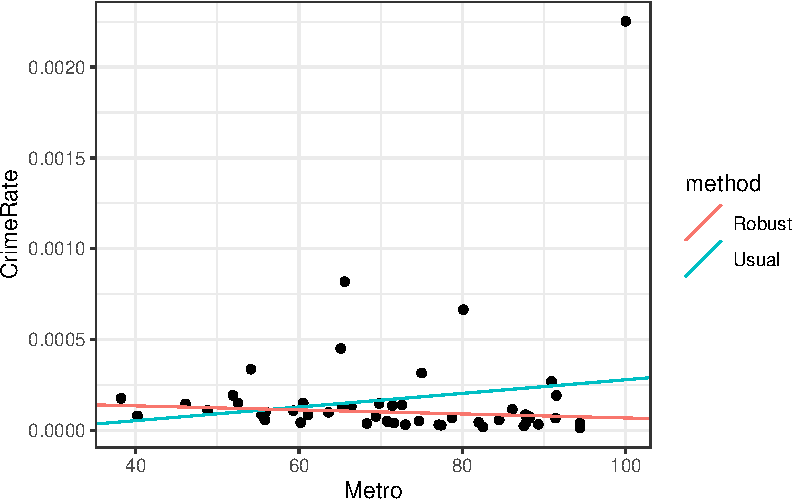
\includegraphics{r-demo-part-3_files/figure-pdf/unnamed-chunk-31-1.pdf}

}

\end{figure}

Next, let's try removing DC and running a usual linear regression.

\begin{Shaded}
\begin{Highlighting}[]
\NormalTok{lm\_fit\_no\_dc }\OtherTok{\textless{}{-}} \FunctionTok{lm}\NormalTok{(CrimeRate }\SpecialCharTok{\textasciitilde{}}\NormalTok{ Metro }\SpecialCharTok{+}\NormalTok{ HighSchool }\SpecialCharTok{+}\NormalTok{ Poverty,}
  \AttributeTok{data =}\NormalTok{ crime\_data }\SpecialCharTok{|\textgreater{}}
    \FunctionTok{filter}\NormalTok{(state\_abbrev }\SpecialCharTok{!=} \StringTok{"DC"}\NormalTok{) }\SpecialCharTok{|\textgreater{}}
    \FunctionTok{column\_to\_rownames}\NormalTok{(}\AttributeTok{var =} \StringTok{"state\_abbrev"}\NormalTok{)}
\NormalTok{)}

\CommentTok{\# residuals versus fitted}
\FunctionTok{plot}\NormalTok{(lm\_fit\_no\_dc, }\AttributeTok{which =} \DecValTok{1}\NormalTok{)}
\end{Highlighting}
\end{Shaded}

\begin{figure}[H]

{\centering 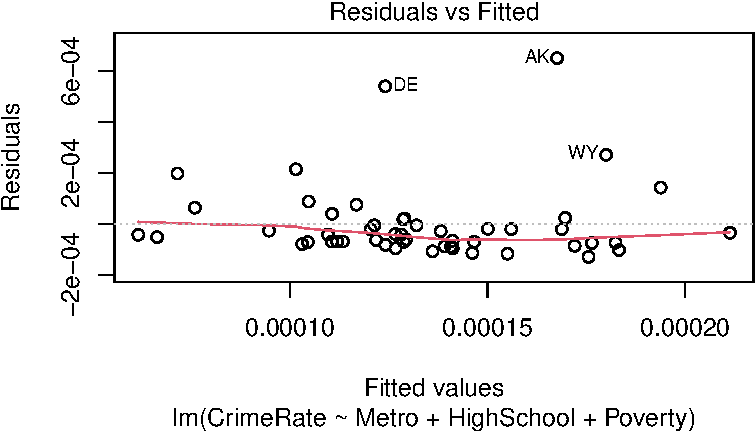
\includegraphics{r-demo-part-3_files/figure-pdf/unnamed-chunk-32-1.pdf}

}

\end{figure}

\begin{Shaded}
\begin{Highlighting}[]
\CommentTok{\# residual QQ plot}
\FunctionTok{plot}\NormalTok{(lm\_fit\_no\_dc, }\AttributeTok{which =} \DecValTok{2}\NormalTok{)}
\end{Highlighting}
\end{Shaded}

\begin{figure}[H]

{\centering 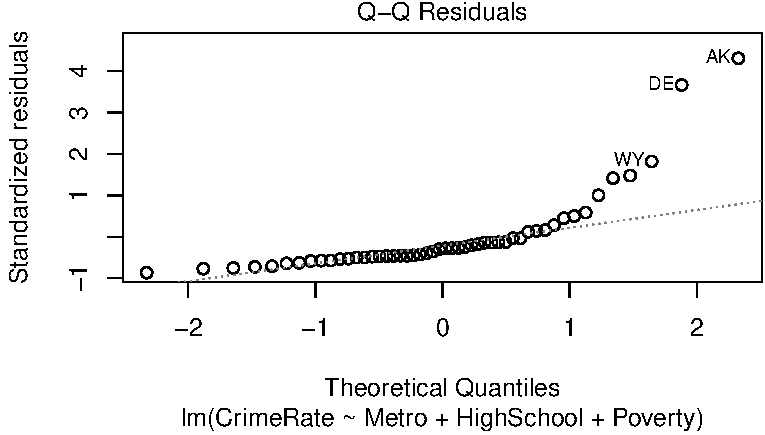
\includegraphics{r-demo-part-3_files/figure-pdf/unnamed-chunk-32-2.pdf}

}

\end{figure}

\begin{Shaded}
\begin{Highlighting}[]
\CommentTok{\# residuals versus leverage (with Cook\textquotesingle{}s distance)}
\FunctionTok{plot}\NormalTok{(lm\_fit\_no\_dc, }\AttributeTok{which =} \DecValTok{5}\NormalTok{)}
\end{Highlighting}
\end{Shaded}

\begin{figure}[H]

{\centering 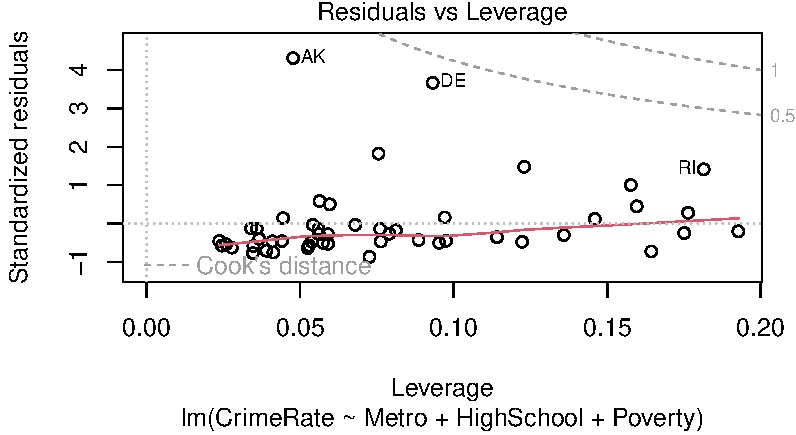
\includegraphics{r-demo-part-3_files/figure-pdf/unnamed-chunk-32-3.pdf}

}

\end{figure}

\part{Generalized linear models: General theory}

Chapters 1-3 focused on the most common class of models used in
applications: linear models. Despite their versatility, linear models do
not apply in all situations. In particular, they are not designed to
deal with binary or count responses. In Chapter 4, we introduce
\emph{generalized linear models} (GLMs), a generalization of linear
models that encompasses a wide variety of incredibly useful models,
including logistic regression and Poisson regression.

We'll start Chapter 4 by introducing exponential dispersion models
(Section Chapter~\ref{sec-edm}), a generalization of the Gaussian
distribution that serves as the backbone of GLMs. Then we formally
define a GLM, demonstrating logistic regression and Poisson regression
as special cases (Section Chapter~\ref{sec-glm-def}). Next, we discuss
maximum likelihood inference in GLMs (Section
Chapter~\ref{sec-glm-max-lik}). Finally, we discuss how to carry out
statistical inference in GLMs (Section Chapter~\ref{sec-glm-inf}).

\hypertarget{sec-edm}{%
\chapter{Exponential dispersion model (EDM)
distributions}\label{sec-edm}}

\hypertarget{definition}{%
\section{Definition}\label{definition}}

Let's start with the Gaussian distribution. If
\(y \sim N(\mu, \sigma^2)\), then it has the following density with
respect to the Lebesgue measure \(\nu\) on \(\mathbb{R}\):

\[
\begin{split}
f_{\mu, \sigma^2}(y) &= \frac{1}{\sqrt{2\pi \sigma^2}}\exp\left(-\frac{1}{2\sigma^2}(y-\mu)^2\right) \\
&= \exp\left(\frac{\mu y - \frac{1}{2}\mu^2}{\sigma^2}\right) \cdot \frac{1}{\sqrt{2\pi \sigma^2}}\exp\left(-\frac1{2\sigma^2} y^2\right).
\end{split}
\]

We can consider a more general class of densities with respect to any
measure \(\nu\):

\begin{equation}\protect\hypertarget{eq-edm-def}{}{
f_{\theta, \phi}(y) \equiv \exp\left(\frac{\theta y - \psi(\theta)}{\phi}\right)h(y, \phi), \quad \theta \in \Theta \subseteq \mathbb{R}, \ \phi > 0.
}\label{eq-edm-def}\end{equation}

Here \(\theta\) is called the \emph{natural parameter}, \(\psi\) is
called the \emph{log-partition function},
\(\Theta \equiv \{\theta: \psi(\theta) < \infty\}\) is called the
natural parameter space,\footnote{The Fisher information is the
  expectation of the Hessian, but for canonical links, the Hessian is
  non-random, so the two coincide.} \(\phi > 0\) is called the
\emph{dispersion parameter}, and \(h\) is called the \emph{base
density}. The distribution with density \(f_{\theta, \phi}\) with
respect to a measure \(\nu\) on \(\mathbb{R}\) is called an
\emph{exponential dispersion model} (EDM).\footnote{If you are not
  familiar with measure theory, you can view \(\nu\) as specifying the
  support of a distribution (the set of values it can take). For
  example, for binary \(y\), \(\nu\) would indicate that \(y\) is
  supported on \(\{0,1\}\), and the ``density'' \(f_{\theta, \phi}\)
  would be a probability mass function.} Sometimes, we parameterize this
distribution using its mean and dispersion, writing

\[
y \sim \text{EDM}(\mu, \phi).
\]

When \(\phi = 1\), the distribution becomes a \emph{one-parameter
natural exponential family} (see Figure~\ref{fig-edms-exp-fams}).

\begin{figure}

{\centering 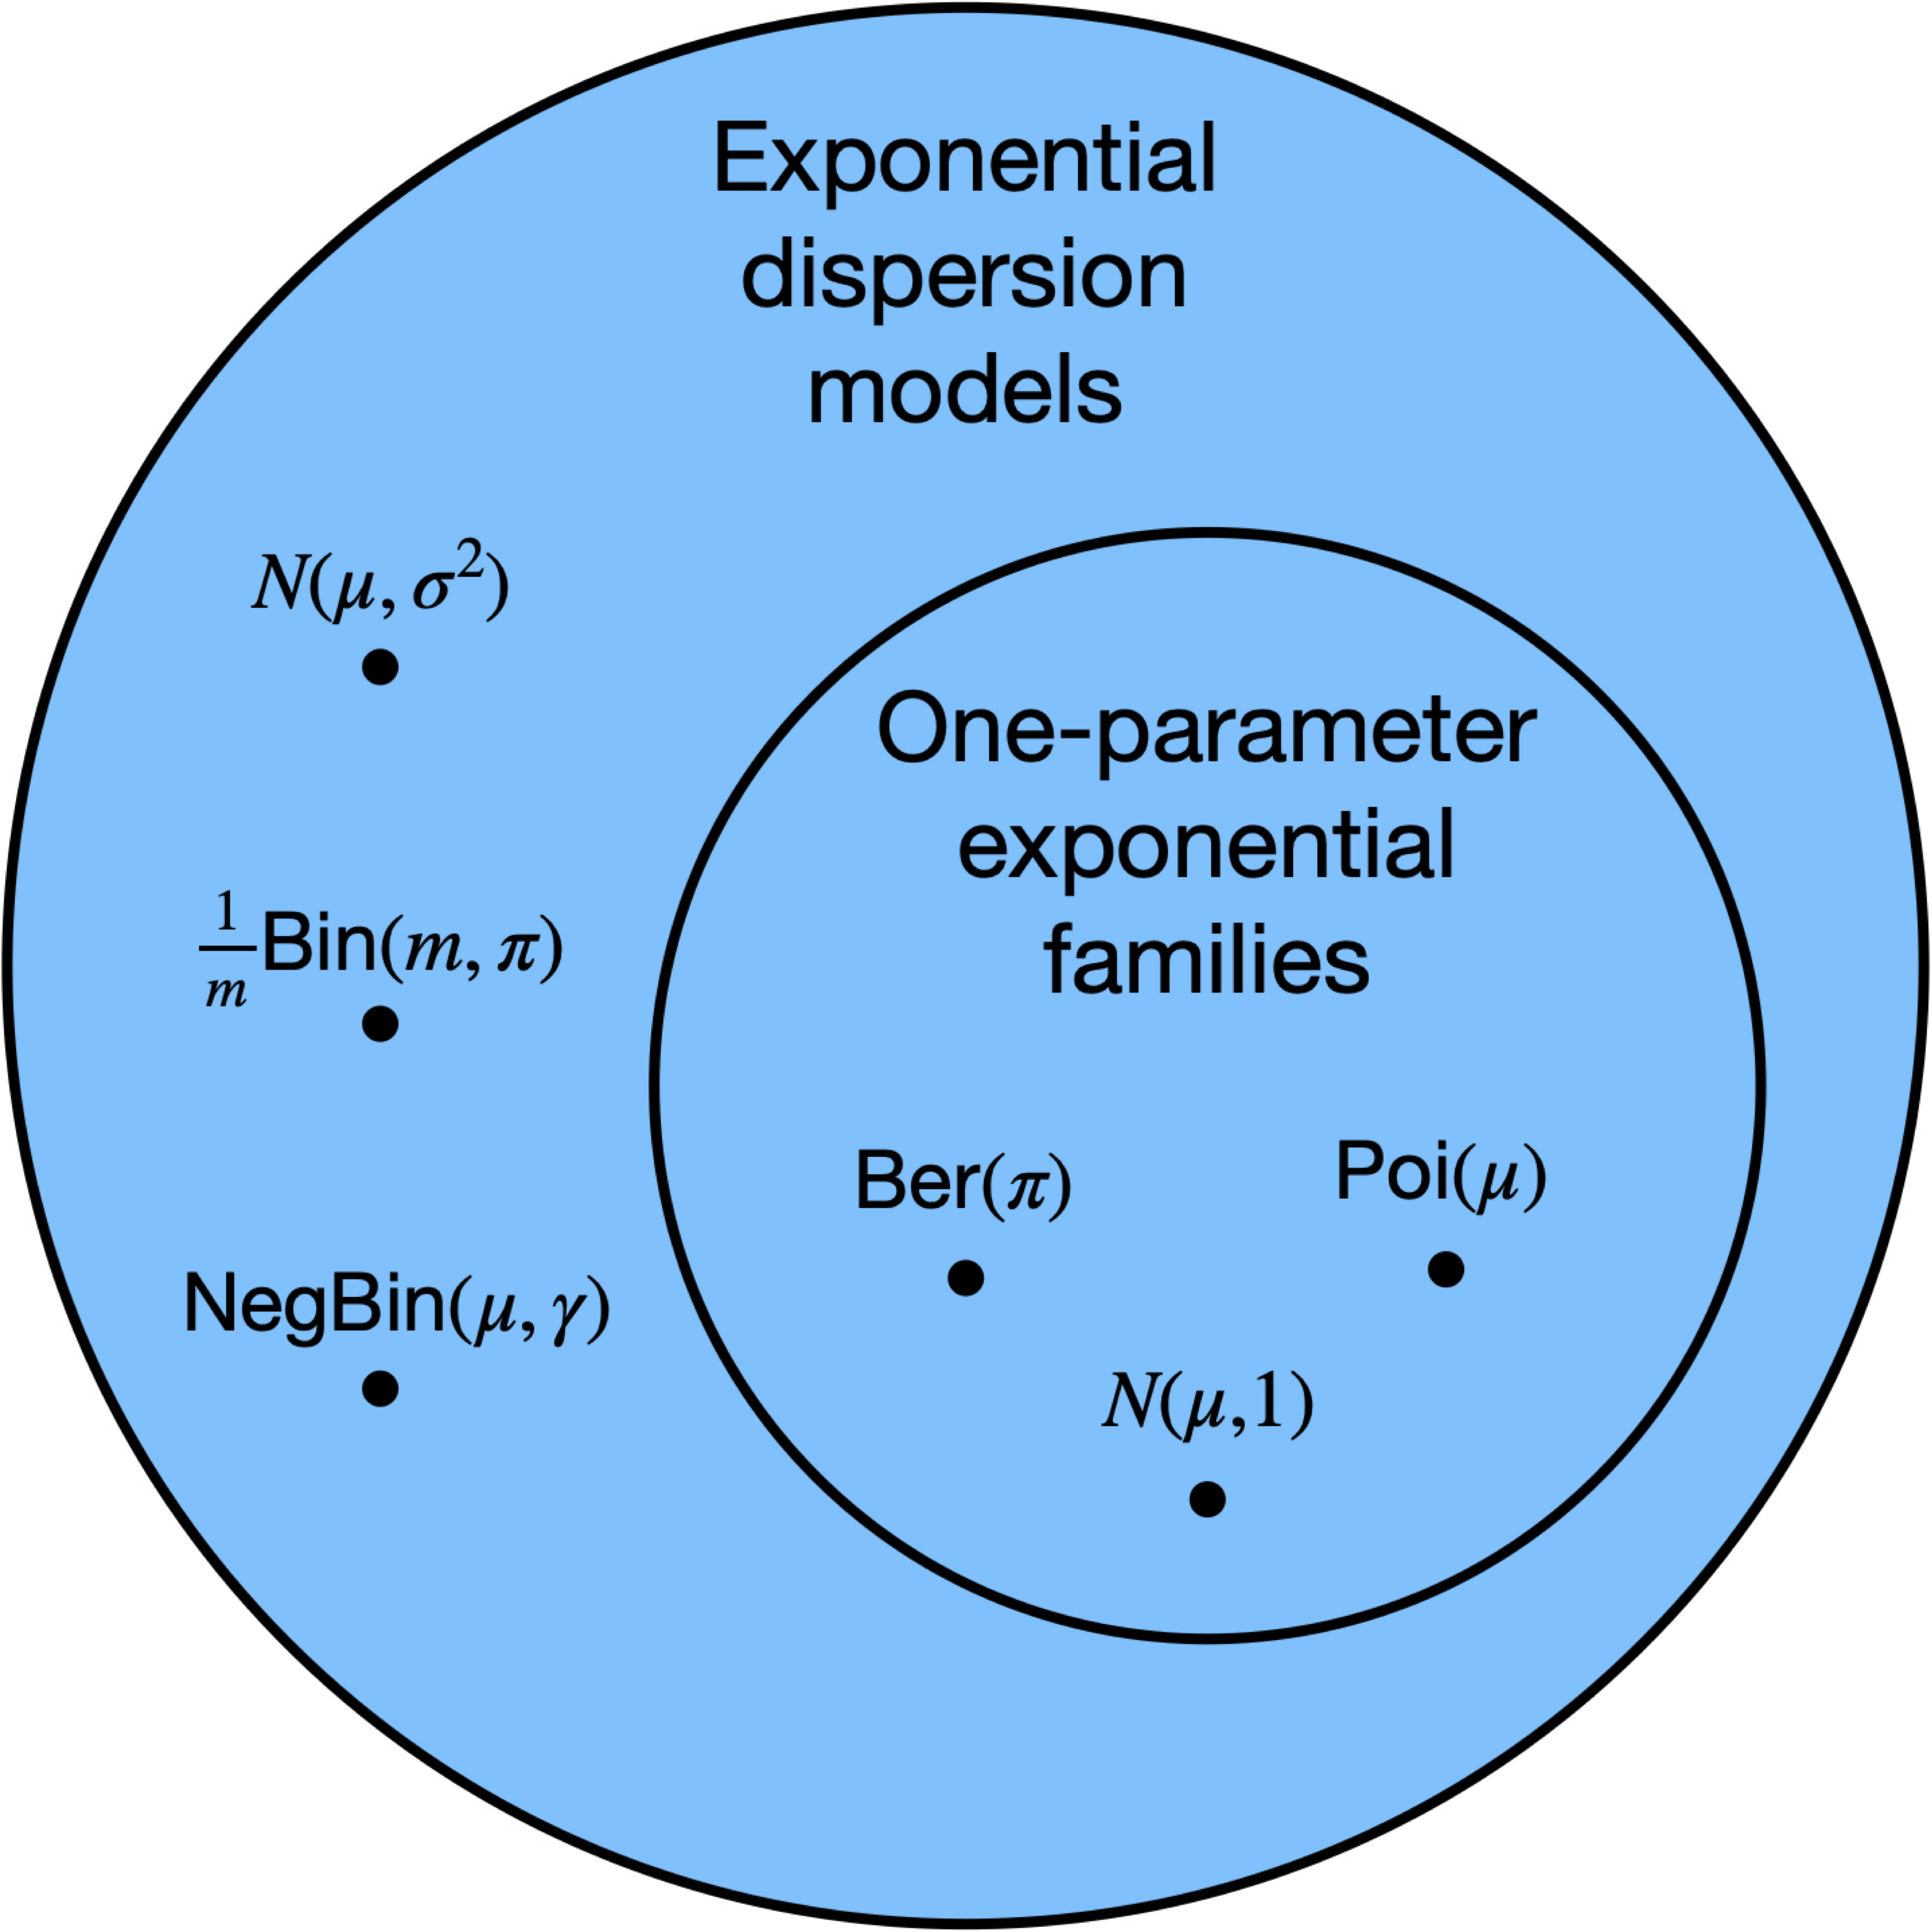
\includegraphics[width=0.5\textwidth,height=\textheight]{figures/edms-exp-fams.png}

}

\caption{\label{fig-edms-exp-fams}Relationship between exponential
dispersion models and one-parameter exponential families.}

\end{figure}

The following proposition presents a useful property of EDMs, which
facilitates inference by ruling out pathological cases.

\begin{proposition}[]\protect\hypertarget{prp-edm-support}{}\label{prp-edm-support}

The support of \(y \sim \text{EDM}(\mu, \phi)\) remains fixed as
\((\mu, \phi)\) vary.

\end{proposition}

\hypertarget{examples}{%
\section{Examples}\label{examples}}

\hypertarget{normal-distribution}{%
\subsection{Normal distribution}\label{normal-distribution}}

As derived above, \(y \sim N(\mu, \sigma^2)\) is an EDM with

\[
\theta = \mu, \quad \psi(\theta) = \frac 12 \theta^2, \quad \phi = \sigma^2, \quad h(y, \phi) = \frac{1}{\sqrt{2\pi \sigma^2}}\exp\left(-\frac1{2\sigma^2} y^2\right).
\]

\hypertarget{bernoulli-distribution}{%
\subsection{Bernoulli distribution}\label{bernoulli-distribution}}

Suppose \(y \sim \text{Ber}(\mu)\). Then, we have

\[
f(y) = \mu^{y}(1-\mu)^{1-y} = \exp\left(y \log \frac{\mu}{1-\mu} + \log(1-\mu) \right).
\]

Therefore, we have \(\theta = \log \frac{\mu}{1-\mu}\), so that
\(\log(1-\mu) = -\log(1+e^\theta)\). It follows that

\[
\theta = \log \frac{\mu}{1-\mu}, \quad \psi(\theta) = \log(1+e^\theta), \quad \phi = 1, \quad h(y) = 1.
\]

Hence, the Bernoulli distribution is an EDM, as well as a one-parameter
exponential family. Note that \(\text{Ber}(0)\) and \(\text{Ber}(1)\)
are not included in this class of EDMs, because there is no
\(\theta \in \Theta = \mathbb{R}\) that gives rise to \(\mu = 0\) or
\(\mu = 1\). Hence, \(\mu \in (0,1)\), and the support of any Bernoulli
EDM is \(\{0,1\}\).

\hypertarget{binomial-distribution}{%
\subsection{Binomial distribution}\label{binomial-distribution}}

Consider the binomial proportion \(y\): \(my \sim \text{Bin}(m, \mu)\).
We have

\[
\begin{split}
f(y) &= {m \choose my}\mu^{my}(1-\mu)^{m(1-y)} \\
&= \exp\left(m\left(y \log \frac{\mu}{1-\mu} + \log(1-\mu)\right)\right){m \choose my},
\end{split}
\]

so

\[
\theta = \log\frac{\mu}{1-\mu}, \quad \psi(\theta) = \log(1+e^\theta), \quad \phi = 1/m, \quad h(y, \phi) = {m \choose my}.
\]

Note that \(\text{Bin}(m, 0)\) and \(\text{Bin}(m, 1)\) are not included
in this class of EDMs, for the same reason as above. Hence,
\(\mu \in (0,1)\), and the support of any binomial EDM is
\(\{0,\frac{1}{m}, \frac{2}{m}, \dots, 1\}\).

\hypertarget{poisson-distribution}{%
\subsection{Poisson distribution}\label{poisson-distribution}}

Suppose \(y \sim \text{Poi}(\mu)\). We have

\[
f(y) = e^{-\mu}\frac{\mu^y}{y!} = \exp(y \log \mu - \mu)\frac{1}{y!}.
\]

Therefore, we have \(\theta = \log \mu\), so that \(\mu = e^\theta\). It
follows that

\[
\theta = \log \mu, \quad \psi(\theta) = e^\theta,\quad \phi = 1, \quad h(y) = \frac{1}{y!}.
\]

Hence, the Poisson distribution is an EDM, as well as a one-parameter
exponential family. Note that \(\text{Poi}(0)\) is not included in this
class of EDMs, because there is no \(\theta \in \Theta = \mathbb{R}\)
that gives rise to \(\mu = 0\). Hence, \(\mu \in (0,\infty)\), and the
support of any Poisson EDM is \(\mathbb{N}\).

Many other examples fall into this class, including the negative
binomial, gamma, and inverse-Gaussian distributions. We will see at
least some of these in the next chapter.

\hypertarget{moments-of-exponential-dispersion-model-distributions}{%
\section{Moments of exponential dispersion model
distributions}\label{moments-of-exponential-dispersion-model-distributions}}

It turns out that the derivatives of the log-partition function \(\psi\)
give the moments of \(y\). Indeed, let's start with the relationship

\[
\int f_{\theta, \phi}(y)d\nu(y) = \int \exp\left(\frac{\theta y - \psi(\theta)}{\phi}\right)h(y, \phi) d\nu(y) = 1.
\]

Differentiating in \(\theta\) and interchanging the derivative and the
integral, we obtain

\[
0 = \frac{d}{d\theta} \int f_{\theta, \phi}(y)dy = \int \frac{y - \dot \psi(\theta)}{\phi}f_{\theta, \phi}(y) dy,
\]

from which it follows that

\begin{equation}\protect\hypertarget{eq-psi-dot}{}{
\dot \psi(\theta) = \int \dot \psi(\theta)f_{\theta, \phi}(y)dy = \int y f_{\theta, \phi}(y)dy = \mathbb{E}[y] \equiv \mu.
}\label{eq-psi-dot}\end{equation}

Thus, the first derivative of the log partition function is the mean of
\(y\). Differentiating again, we get

\[
\begin{split}
\phi \cdot \ddot \psi(\theta) &= \phi \int \ddot \psi(\theta) f_{\theta, \phi}(y) d\nu(y) \\
&= \int (y - \dot \psi(\theta))^2 f_{\theta, \phi}(y) dy = \int (y - \mu)^2f_{\theta, \phi}(y) d\nu(y) \\
&= \text{Var}[y].
\end{split}
\]

Thus, the second derivative of the log-partition function multiplied by
the dispersion parameter is the variance of \(y\). The following
proposition summarizes these results.

\begin{proposition}[EDM
moments]\protect\hypertarget{prp-moments-edm}{}\label{prp-moments-edm}

If \(y \sim \text{EDM}(\mu, \phi)\), then \[
\mathbb E[y] = \dot \psi(\theta), \quad \text{Var}[y] = \phi \cdot \ddot \psi(\theta).
\]

\end{proposition}

\hypertarget{relationships-among-the-mean-variance-and-natural-parameter}{%
\section{Relationships among the mean, variance, and natural
parameter}\label{relationships-among-the-mean-variance-and-natural-parameter}}

\hypertarget{relationship-between-the-mean-and-the-natural-parameter}{%
\subsection{Relationship between the mean and the natural
parameter}\label{relationship-between-the-mean-and-the-natural-parameter}}

The log-partition function \(\psi\) induces a connection
(\ref{eq-psi-dot}) between the natural parameter \(\theta\) and the mean
\(\mu\). Because

\begin{equation}\protect\hypertarget{eq-dmu-dtheta}{}{
\frac{d\mu}{d\theta} = \frac{d}{d\theta}\dot \psi(\theta) = \ddot \psi(\theta) = \frac{1}{\phi}\text{Var}[y] > 0,
}\label{eq-dmu-dtheta}\end{equation}

it follows that \(\mu\) is a strictly increasing function of \(\theta\),
so in particular the mapping between \(\mu\) and \(\theta\) is
bijective. Therefore, we can think of equivalently parameterizing the
distribution via \(\mu\) or \(\theta\).

\hypertarget{relationship-between-the-mean-and-variance}{%
\subsection{Relationship between the mean and
variance}\label{relationship-between-the-mean-and-variance}}

Note that the mean of an EDM, together with the dispersion parameter,
determines its variance (since it determines the natural parameter
\(\theta\)). Define

\[
V(\mu) \equiv \frac{d\mu}{d\theta},
\]

so that \(\text{Var}[y] = \phi V(\mu)\). For example, a Poisson random
variable with mean \(\mu\) has variance \(\mu\) and a Bernoulli random
variable with mean \(\mu\) has \(V(\mu) = \mu(1-\mu)\). The
mean-variance relationship turns out to characterize the EDM, i.e.~an
EDM with mean equal to its variance is the Poisson distribution. For all
EDMs except the normal distribution, the variance depends nontrivially
on the mean. Therefore, heteroskedasticity is a natural feature of EDMs
(rather than a pathology that needs to be corrected for).

\hypertarget{the-unit-deviance}{%
\section{The unit deviance}\label{the-unit-deviance}}

A key quantity in the analysis of normal linear regression models is
\((y, \mu) \mapsto (y - \mu)^2\), which is a notion of distance between
the parameter \(\mu\) and the observation \(y\). The \emph{unit
deviance} is a generalization of this quantity to EDMs. As a starting
point, consider the log-likelihood of an EDM: \[
\ell(y, \mu) = \frac{\theta y - \psi(\theta)}{\phi} + \log h(y, \phi) = \frac{\theta(\mu) y - \psi(\theta(\mu))}{\phi} + \log h(y, \phi),
\] where \(\theta(\mu) = \dot \psi^{-1}(\mu)\), recalling the
relationship (\ref{eq-psi-dot}). The quantity \(\ell(y, \mu)\) is larger
to the extent that \(\mu\) is a better fit for \(y\). Furthermore, it is
easy to verify that \(\mu \mapsto \ell(y, \mu)\) is maximized by
\(\mu = y\). Motivated by this observation, we calculate that twice the
log-likelihood ratio between \(\mu = \mu\) and \(\mu = y\) is
\begin{equation}\protect\hypertarget{eq-unit-deviance}{}{
\begin{split}
&2(\ell(y, y) - \ell(y, \mu)) \\
&\quad= \frac{2\{[\theta(y) y - \psi(\theta(y))] - [\theta(\mu) y - \psi(\theta(\mu))]\}}{\phi} \\
&\quad\equiv \frac{d(y, \mu)}{\phi}.
\end{split}
}\label{eq-unit-deviance}\end{equation} The quantity in the numerator is
the \emph{unit deviance} \(d(y, \mu)\), defined as the dispersion
\(\phi\) times twice the log-likelihood ratio between \(y\) and \(\mu\).
As we will see in Section~\ref{sec-normal-deviance}, \(d(y, \mu)\)
generalizes the quantity \((y - \mu)^2\) for the normal distribution.
The following proposition summarizes a few key properties of the unit
deviance.

\begin{proposition}[Unit deviance
properties]\protect\hypertarget{prp-unit-deviance}{}\label{prp-unit-deviance}

When viewed as a function of \(\mu\), the unit deviance \(d(y, \mu)\) is
nonnegative function that achieves a unique global minimum of zero for
\(\mu = y\) and increases as \(\mu\) moves away from \(y\).

\end{proposition}

\begin{proof}

Differentiating \(d(y, \mu)\) in \(\mu\), we have \[
\frac{\partial d(y, \mu)}{\partial \mu} = \frac{\partial d(y, \mu)}{\partial \theta} \frac{\partial \theta}{\partial \mu} = \frac{\mu - y}{V(\mu)}.
\] Since \(V(\mu) > 0\), this establishes that \(d(y, \mu)\) decreases
on \(\mu \in (\infty, y)\) and then increases on \((y, \infty)\),
Therefore, \(d(y, \mu) \geq d(y, y) = 0\) for all \(\mu\).

\end{proof}

\hypertarget{sec-normal-deviance}{%
\subsection{Example: Normal distribution}\label{sec-normal-deviance}}

For the normal distribution, we have \(\theta = \mu\) and
\(\psi(\theta) = \frac12 \theta^2\). Therefore, \[
\begin{split}
d(y, \mu) &= 2\{[\theta(y) y - \psi(\theta(y))] - [\theta(\mu) y - \psi(\theta(\mu))]\} \\
&= 2\{[y^2 - \tfrac12 y^2] - [\mu y - \tfrac12 \mu^2]\} \\
&= (y - \mu)^2.
\end{split}
\] Figure~\ref{fig-normal-unit-deviance} displays an example of the
normal unit deviance.

\begin{figure}

{\centering 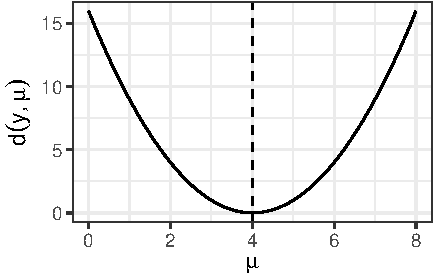
\includegraphics{exponential-dispersion-models_files/figure-pdf/fig-normal-unit-deviance-1.pdf}

}

\caption{\label{fig-normal-unit-deviance}The normal unit deviance for
\(y = 4\).}

\end{figure}

\hypertarget{example-poisson-distribution}{%
\subsection{Example: Poisson
distribution}\label{example-poisson-distribution}}

For the Poisson distribution, we have \(\theta = \log \mu\) and
\(\psi(\theta) = e^\theta\), so

\[
\begin{split}
d(y, \mu) &= 2\{[\theta(y) y - \psi(\theta(y))] - [\theta(\mu) y - \psi(\theta(\mu))]\} \\
&= 2\{[y\log y - y] - [y \log \mu - \mu]\} \\
&= 2\left(y\log \frac{y}{\mu} - (y - \mu)\right).
\end{split}
\]

See Figure~\ref{fig-poisson-unit-deviance} for an example of the shape
of this function.

\begin{figure}

{\centering 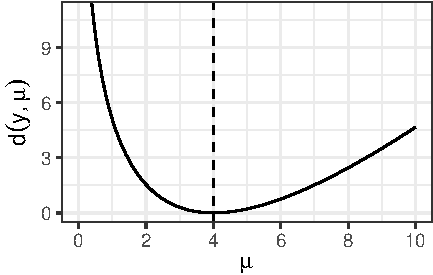
\includegraphics{exponential-dispersion-models_files/figure-pdf/fig-poisson-unit-deviance-1.pdf}

}

\caption{\label{fig-poisson-unit-deviance}The Poisson unit deviance for
\(y = 4\).}

\end{figure}

Note that the Poisson deviance is asymmetric about \(\mu = y\). This is
a consequence of the nontrivial mean-variance relationship for the
Poisson distribution. In particular, the Poisson distribution's variance
grows with its mean. Therefore, an observation of \(y = 4\) is less
likely to have come from a Poisson distribution with mean \(\mu = 2\)
than from a Poisson distribution with mean \(\mu = 6\).

\hypertarget{small-dispersion-approximations-to-an-edm}{%
\section{Small-dispersion approximations to an
EDM}\label{small-dispersion-approximations-to-an-edm}}

If the dispersion \(\phi\) is small, then that means that \(y\) is a
fairly precise estimate of \(\mu\), similar to an average of multiple
independent samples from a mean-\(\mu\) distribution. Consider, for
example, that \(\frac{1}{m}\text{Bin}(m, \mu)\) is the mean of \(m\)
i.i.d. draws from \(\text{Ber}(\mu)\). In this case, we can use either
the normal approximation or the saddlepoint approximation to approximate
the EDM density. For the sake of this section, we will abuse notation by
denoting by \(f_{\mu, \phi}\) the EDM with mean \(\mu\) and dispersion
\(\phi\).

\hypertarget{the-normal-approximation}{%
\subsection{The normal approximation}\label{the-normal-approximation}}

\hypertarget{the-approximation}{%
\subsubsection{The approximation}\label{the-approximation}}

For small values of \(\phi\), we can hope to approximate
\(f_{\mu, \phi}\) with a normal distribution. Recall that the mean and
variance of this distribution are \(\mu\) and \(\phi \cdot V(\mu)\),
respectively. The central limit theorem gives

\[
\frac{y - \mu}{\sqrt{\phi \cdot V(\mu)}} \rightarrow_d N(0,1) \quad \text{as} \quad \phi \rightarrow 0,
\]

so

\[
y \overset \cdot \sim N(\mu, \phi \cdot V(\mu)) \equiv \tilde f^{\text{normal}}_{\mu, \phi}.
\]

For example, we have

\[
\text{Poi}(\mu) \approx N(\mu, \mu).
\]

For the normal EDM, note that the normal approximation is exact. One
consequence of the normal approximation is

\begin{equation}\protect\hypertarget{eq-clt-chi-squared}{}{
\frac{(y - \mu)^2}{\phi \cdot V(\mu)} \overset \cdot \sim \chi^2_1.
}\label{eq-clt-chi-squared}\end{equation}

This fact will be useful to us as we carry out inference for GLMs.

\hypertarget{sec-normal-approx-accuracy}{%
\subsubsection{Normal approximation
accuracy}\label{sec-normal-approx-accuracy}}

We have

\[
\tilde f^{\text{normal}}_{\mu, \phi}(y) = f_{\mu, \phi}(y) + O(\sqrt{\phi}).
\]

In practice, the rule of thumb for the applicability of this
approximation to get statements like (\ref{eq-clt-chi-squared}) is that

\[
\tau \equiv \frac{\phi \cdot V(\mu)}{(\mu - \text{boundary})^2} \leq \frac{1}{5}.
\]

Here, ``boundary'' represents the nearest boundary of the parameter
space to \(\mu\). For example, if
\(y \sim \frac{1}{m}\text{Bin}(m, \mu)\), then we have

\[
\begin{split}
\tau &= \frac{\frac{1}{m} \cdot \mu \cdot (1-\mu)}{\min(\mu, 1-\mu)^2} \\
&= \frac{1}{m} \cdot \max\left(\frac{\mu}{1-\mu}, \frac{1-\mu}{\mu}\right) \\
&\approx \frac{1}{m} \cdot \max\left(\frac 1 \mu, \frac 1 {1-\mu}\right),
\end{split}
\]

so \(\tau \leq 1/5\) roughly if \(m \mu \leq 5\) and
\(m (1-\mu) \leq 5\). For Poisson distributions, we always have
\(\tau = 1\), but for some reason small-dispersion asymptotics still
applies as \(\mu \rightarrow \infty\) as opposed to
\(\tau \rightarrow 0\). The criterion \(\tau \leq 1/5\) is satisfied
when \(\mu \leq 5\).

\hypertarget{the-saddlepoint-approximation}{%
\subsection{The saddlepoint
approximation}\label{the-saddlepoint-approximation}}

\hypertarget{the-approximation-1}{%
\subsubsection{The approximation}\label{the-approximation-1}}

Another approximation to the EDM density is the saddlepoint
approximation, which tends to be more accurate than the normal
approximation. The reason the normal approximation may be inaccurate is
that the quality of the central limit approximation degrades as one
enters the tails of the distribution. In particular, the normal
approximation to \(f_{\mu, \phi}(y)\) may be poor if \(\mu\) is far from
\(y\). The saddlepoint approximation is built on the observation that
the EDM density for \(f_{\mu, \phi}(y)\) can be written in terms of the
density \(f_{y, \phi}(y)\); the latter density is by definition
evaluated at its mean. Indeed,

\begin{equation}\protect\hypertarget{eq-deviance-form}{}{
\begin{split}
f_{\mu, \phi}(y) &\equiv \exp\left(\frac{\theta y - \psi(\theta)}{\phi}\right)h(y, \phi) \\
&= \exp\left(-\frac{d(y, \mu)}{2\phi}\right)\exp\left(\frac{\theta(y) y - \psi(\theta(y))}{\phi}\right) h(y, \phi) \\
&= \exp\left(-\frac{d(y, \mu)}{2\phi}\right)f_{y, \phi}(y).
\end{split}
}\label{eq-deviance-form}\end{equation}

Now, we apply the central limit theorem to approximate
\(f_{y, \phi}(y)\):

\[
f_{y, \phi}(y) \approx \frac{1}{\sqrt{2\pi \phi V(y)}}.
\]

Substituting this approximation into (\ref{eq-deviance-form}), we obtain
the \emph{saddlepoint approximation}:

\[
f_{\mu, \phi}(y) \approx \frac{1}{\sqrt{2\pi \phi V(y)}}\exp\left(-\frac{d(y, \mu)}{2\phi}\right) \equiv \widetilde f^{\text{saddle}}_{\mu, \phi}(y).
\]

For the normal EDM, note that the normal approximation is exact. For the
Poisson distribution, we get

\[
\widetilde f^{\text{saddle}}_{\mu, \phi}(y) = \frac{1}{\sqrt{2\pi y}}\exp\left(-y \log \frac y \mu + (y - \mu)\right).
\]

The approximation can be shown to lead to the following consequence:

\begin{equation}\protect\hypertarget{eq-spa-chi-squared}{}{
\frac{d(y, \mu)}{\phi} \overset \cdot \sim \chi^2_1.
}\label{eq-spa-chi-squared}\end{equation}

Here, we are using the unit deviance rather than the squared distance to
measure the deviation of \(\mu\) from \(y\). This fact will be useful to
us as we carry out inference for GLMs.

\hypertarget{sec-saddlepoint-approximation-accuracy}{%
\subsubsection{Saddlepoint approximation
accuracy}\label{sec-saddlepoint-approximation-accuracy}}

We have still used a normal approximation, but this time we have used it
to approximate \(f_{y, \phi}(y)\) instead of \(f_{\mu, \phi}(y)\). Since
the normal approximation is applied to a distribution (\(f_{y, \phi}\))
at its mean, we expect it to be more accurate than a normal
approximation applied to a distribution (\(f_{\mu, \phi}\)) at a point
potentially far from its mean. The saddlepoint approximation yields an
approximation to the density that is \emph{multiplicative} rather than
\emph{additive}, and of order \(O(\phi)\) rather than
\(O(\sqrt{\phi})\):

\[
\tilde f^{\text{saddle}}_{\mu, \phi}(y) = f_{\mu, \phi}(y) \cdot (1 + O(\phi)).
\]

In practice, the rule of thumb for the applicability of this
approximation to get statements like (\ref{eq-spa-chi-squared}) is that
\(\tau \leq 1/3\); the looser requirement on \(\tau\) reflects the
greater accuracy of the saddlepoint approximation. This translates to
\(m\mu \geq 3\) and \(m(1-\mu) \geq 3\) for the binomial and
\(\mu \geq 3\) for the Poisson.

\hypertarget{comparing-the-two-approximations}{%
\subsection{Comparing the two
approximations}\label{comparing-the-two-approximations}}

The saddlepoint approximation is more accurate than the normal
approximation, as discussed above. However, the accuracy of the
saddlepoint approximation relies on the assumption that the entire
parametric form of the EDM is correctly specified. On the other hand,
the accuracy of the normal distribution requires only that the first two
moments of the EDM are correctly specified.

\hypertarget{sec-glm-def}{%
\chapter{GLM definition}\label{sec-glm-def}}

In this class, the focus is on building models that tie a vector of
predictors \((\boldsymbol x_{i*})\) to a response \(y_i\). For linear
regression, the mean of \(y\) was modeled as a linear combination of the
predictors \(\boldsymbol x_{i*}^T \boldsymbol{\beta}\):
\(\mu_i = \boldsymbol x_{i*}^T \boldsymbol{\beta}\). More generally, we
might want to model \emph{a function} of the mean \(\eta_i = g(\mu_i)\)
as a linear combination of the predictors; \(g\) is called the
\emph{link function} and \(\eta_i\) the \emph{linear predictor}. Pairing
a link function with an EDM gives us a \emph{generalized linear model}
(GLM):

\hypertarget{definition-1}{%
\section{Definition}\label{definition-1}}

We define \(\{(y_i, \boldsymbol x_{i*})\}_{i = 1}^n\) as following a
generalized linear model based on the exponential dispersion model
\(f_{\theta, \phi}\), monotonic and differentiable link function \(g\),
offset terms \(o_i \in \mathbb R\), and observation weights \(w_i > 0\)
if

\begin{equation}\protect\hypertarget{eq-glm-def}{}{
y_i \overset{\text{ind}} \sim \text{EDM}(\mu_i, \phi_0/w_i), \quad \eta_i \equiv g(\mu_i) = o_i + \boldsymbol x^T_{i*}\boldsymbol{\beta}.
}\label{eq-glm-def}\end{equation}

The offset terms \(o_i\) and observation weights \(w_i\) are both known
in advance. The free parameters in a GLM are the coefficients
\(\boldsymbol{\beta}\) and, possibly, the parameter \(\phi_0\)
controlling the dispersion. We will see examples where \(\phi_0\) is
known (e.g.~Poisson regression) and those where \(\phi_0\) is unknown
(e.g.~linear regression).

The ``default'' choice for the link function \(g\) is the
\emph{canonical link function}

\[
g(\mu) = \dot \psi^{-1}(\mu),
\]

which, given the relationship (\ref{eq-psi-dot}), gives
\(\eta = \dot \psi^{-1}(\mu) = \theta\), i.e.~the linear predictor
coincides with the natural parameter. As discussed in the context of
equation (\ref{eq-dmu-dtheta}), \(\dot \psi^{-1}\) is a valid link
function because it is monotonic and differentiable. Canonical link
functions are very commonly used with GLMs because they lead to various
nice properties that general GLMs do not enjoy (e.g.~concave
log-likelihood).

\hypertarget{examples-1}{%
\section{Examples}\label{examples-1}}

\hypertarget{example-linear-regression-model}{%
\subsection{Example: Linear regression
model}\label{example-linear-regression-model}}

The linear regression model is a special case of a GLM, with
\(\phi_0 = \sigma^2\) (unknown), \(w_i = 1\), \(o_i = 0\), and identity
(canonical) link function:

\[
y_i \overset{\text{ind}}\sim N(\mu_i, \sigma^2); \quad \eta_i = \mu_i = \boldsymbol x_{i*}^T \boldsymbol{\beta}.
\]

\hypertarget{example-weighted-linear-regression-model}{%
\subsection{Example: Weighted linear regression
model}\label{example-weighted-linear-regression-model}}

If each observation \(y_i\) is the mean of \(m_i\) independent repeated
observations, then we get a weighted linear regression model, with
\(\phi_0 = \sigma^2\) (unknown), \(w_i = m_i\), \(o_i = 0\), and
identity (canonical) link function:

\[
y_i \overset{\text{ind}}\sim N(\mu_i, {\textstyle \frac{\sigma^2}{m_i}}); \quad \eta_i = \mu_i = \boldsymbol x_{i*}^T \boldsymbol{\beta}.
\]

\hypertarget{example-ungrouped-logistic-regression-model}{%
\subsection{Example: Ungrouped logistic regression
model}\label{example-ungrouped-logistic-regression-model}}

The \emph{ungrouped logistic regression model} is the GLM based on the
Bernoulli EDM with \(\phi_0 = 1\) (known), \(w_i = 1\), \(o_i = 0\), and
the canonical link function:

\[
y_i \overset{\text{ind}}\sim \text{Ber}(\mu_i); \quad \eta_i = \theta_i = \log\frac{\mu_i}{1-\mu_i} = \boldsymbol x_{i*}^T \boldsymbol{\beta}.
\]

Thus the canonical link function for logistic regression is the
\emph{logistic link function} \(g(\mu) = \log \frac{\mu}{1-\mu}\).

\hypertarget{example-grouped-logistic-regression-model}{%
\subsection{Example: Grouped logistic regression
model}\label{example-grouped-logistic-regression-model}}

Suppose \(y_i\) is a binomial proportion based on \(m_i\) trials. The
\emph{grouped logistic regression model} is the GLM based on the
binomial EDM with \(\phi_0 = 1\) (known), \(w_i = 1/m_i\), \(o_i = 0\),
and the canonical link function:

\[
m_i y_i \sim \text{Bin}(m_i, \mu_i); \quad \eta_i = \log \frac{\mu_i}{1-\mu_i} = o_i + \boldsymbol x^T_{i*}\boldsymbol{\beta}.
\]

Note that a binomial proportion \(y_i\) based on \(m_i\) trials and a
success probability of \(\mu_i\) can be equivalently represented as
\(m_i\) independent Bernoulli draws with the same success probability
\(\mu_i\). Therefore, any grouped logistic regression model can be
equivalently represented as an ungrouped logistic regression model with
\(\sum_{i = 1}^n m_i\) observations. We will see that, despite this
equivalence, grouped logistic regression models have some useful
properties that ungrouped logistic regression models do not.

\hypertarget{example-poisson-regression-model}{%
\subsection{Example: Poisson regression
model}\label{example-poisson-regression-model}}

\emph{Poisson regression} is the Poisson EDM with \(\phi_0 = 1\)
(known), \(w_i = 1\), \(o_i = 0\), and the canonical link function:

\[
y_i \overset{\text{ind}}\sim \text{Poi}(\mu_i); \quad \eta_i = \theta_i = \log \mu_i = \boldsymbol x_{i*}^T \boldsymbol{\beta}.
\]

Thus the canonical link function for Poisson regression is the \emph{log
link function} \(g(\mu) = \log \mu\).

\hypertarget{sec-glm-max-lik}{%
\chapter{Parameter estimation}\label{sec-glm-max-lik}}

\hypertarget{sec-glm-likelihood}{%
\section{The GLM likelihood, score, and Fisher
information}\label{sec-glm-likelihood}}

The log-likelihood of a GLM is:

\begin{equation}\protect\hypertarget{eq-glm-log-likelihood}{}{
\log \mathcal L(\boldsymbol{\beta}) = \sum_{i = 1}^n \frac{\theta_i y_i - \psi(\theta_i)}{\phi_0/w_i} + \sum_{i = 1}^n \log h(y_i, \phi_0/w_i).
}\label{eq-glm-log-likelihood}\end{equation}

Let's differentiate this with respect to \(\boldsymbol{\beta}\), using
the chain rule:

\[
\begin{split}
  \frac{\partial \log \mathcal L(\boldsymbol{\beta})}{\partial \boldsymbol{\beta}} &= \frac{\partial \log \mathcal L(\boldsymbol{\beta})}{\partial \boldsymbol{\theta}}\frac{\partial \boldsymbol{\theta}}{\partial \boldsymbol{\mu}} \frac{\partial \boldsymbol{\mu}}{\partial \boldsymbol{\eta}}\frac{\partial \boldsymbol{\eta}}{\partial \boldsymbol{\beta}} \\
  &=  (\boldsymbol{y} - \boldsymbol{\mu})^T \text{diag}(\phi_0/w_i)^{-1} \cdot \text{diag}(\ddot{\psi}(\theta_i))^{-1} \cdot \text{diag}\left(\frac{\partial\mu_i}{\partial \eta_i}\right) \cdot \boldsymbol{X}\\
  &= \frac{1}{\phi_0}(\boldsymbol{y} - \boldsymbol{\mu})^T \text{diag}\left(\frac{w_i}{V(\mu_i)(d\eta_i/d\mu_i)^2}\right)\cdot \text{diag}\left(\frac{\partial\eta_i}{\partial \mu_i}\right) \cdot \boldsymbol{X} \\
  &\equiv \frac{1}{\phi_0}(\boldsymbol{y} - \boldsymbol{\mu})^T \boldsymbol{W} \boldsymbol{M} \boldsymbol{X}.
\end{split}
\]

Here, \(\boldsymbol{W} \equiv \text{diag}(W_i)\) is a diagonal matrix of
\emph{working weights} and
\(\boldsymbol{M} \equiv \text{diag}\left(\frac{\partial\eta_i}{\partial \mu_i}\right) = \text{diag}(g'(\mu_i))\)
is a diagonal matrix of link derivatives. Transposing, we get the score
vector:

\begin{equation}\protect\hypertarget{eq-glm-score}{}{
\boldsymbol{U}(\boldsymbol{\beta}) = \frac{1}{\phi_0}\boldsymbol{X}^T \boldsymbol{M} \boldsymbol{W} (\boldsymbol{y} - \boldsymbol{\mu}).
}\label{eq-glm-score}\end{equation}

To get the Fisher information matrix, note first that:

\begin{equation}\protect\hypertarget{eq-glm-variance-y}{}{
\text{Var}[\boldsymbol{y}] = \text{diag}\left(\phi_0\frac{V(\mu_i)}{w_i}\right) = \phi_0 \boldsymbol{W}^{-1} \boldsymbol{M}^{-2}
}\label{eq-glm-variance-y}\end{equation}

we can compute the covariance matrix of the score vector:

\begin{equation}\protect\hypertarget{eq-glm-fisher-info}{}{
\begin{split}
\boldsymbol{I}(\boldsymbol{\beta}) = \text{Var}[\boldsymbol{U}(\boldsymbol{\beta})] &= \frac{1}{\phi^2_0}\boldsymbol{X}^T \boldsymbol{M} \boldsymbol{W} \text{Var}[\boldsymbol{y}] \boldsymbol{M} \boldsymbol{W} \boldsymbol{X} \\
&= \frac{1}{\phi^2_0}\boldsymbol{X}^T \boldsymbol{M} \boldsymbol{W} \phi_0 \boldsymbol{W}^{-1}\boldsymbol{M}^{-2} \boldsymbol{M} \boldsymbol{W} \boldsymbol{X} \\
&= \frac{1}{\phi_0}\boldsymbol{X}^T \boldsymbol{W} \boldsymbol{X}.
\end{split}
}\label{eq-glm-fisher-info}\end{equation}

\hypertarget{sec-mle-glm}{%
\section{\texorpdfstring{Maximum likelihood estimation of
\(\boldsymbol{\beta}\)}{Maximum likelihood estimation of \textbackslash boldsymbol\{\textbackslash beta\}}}\label{sec-mle-glm}}

To estimate \(\boldsymbol{\beta}\), we can set the score vector to zero:

\[
\frac{1}{\phi_0}\boldsymbol{X}^T \widehat{\boldsymbol{M}} \widehat{\boldsymbol{W}} (\boldsymbol{y} - \widehat{\boldsymbol{\mu}}) = 0 \quad \Longleftrightarrow \quad \boldsymbol{X}^T \text{diag}\left(\frac{w_i}{V(\widehat \mu_i)g'(\widehat \mu_i)}\right)(\boldsymbol{y} - \widehat{\boldsymbol{\mu}}) = 0.
\]

These equations are called the \emph{normal equations}. Unfortunately,
unlike least squares, the normal equations cannot be solved analytically
for \(\widehat{\boldsymbol{\beta}}\). They are solved numerically
instead; see Section~\ref{sec-irls}. Note that \(\phi_0\) cancels from
the normal equations, and therefore the coefficients
\(\boldsymbol{\beta}\) can be estimated without estimating the
dispersion. Recall that we have seen this phenomenon for least squares.
Also note that the normal equations simplify when the canonical link
function is used, so that \(\eta_i = \theta_i\). Assuming additionally
that \(w_i = 1\), we get:

\[
\boldsymbol{\widehat M} \boldsymbol{\widehat W} = \text{diag}\left(\frac{\widehat{\partial \mu_i/\partial \theta_i}}{V(\widehat \mu_i)}\right) = \frac{\ddot{\psi}(\widehat \theta_i)}{\ddot{\psi}(\widehat \theta_i)} = 1,
\]

so the normal equations reduce to:

\begin{equation}\protect\hypertarget{eq-canonical-normal-equations}{}{
\boldsymbol{X}^T (\boldsymbol{y} - \widehat{\boldsymbol{\mu}}) = 0.
}\label{eq-canonical-normal-equations}\end{equation}

We recognize these as the normal equation for linear regression. Since
both ungrouped logistic regression and Poisson regression also use
canonical links and have unit weights, the simplified normal equations
(\ref{eq-canonical-normal-equations}) apply to the latter regressions as
well.

In the linear regression case, we interpreted the normal equations
(\ref{eq-canonical-normal-equations}) as an orthogonality statement:
\(\boldsymbol{y} - \widehat{\boldsymbol{\mu}} \perp C(\boldsymbol{X})\).
In the case of GLMs, the set
\(C(\boldsymbol{X}) \equiv \{\boldsymbol{\mu} = \mathbb{E}[\boldsymbol{y}]: \boldsymbol{\beta} \in \mathbb{R}^p\}\)
is no longer a linear space. In fact, it is a nonlinear transformation
of the column space of \(\boldsymbol{X}\) (a \(p\)-dimensional manifold
in \(\mathbb{R}^n\)):

\[
C(\boldsymbol{X}) \equiv \{\boldsymbol{\mu} = \mathbb{E}[\boldsymbol{y}]: \boldsymbol{\beta} \in \mathbb{R}^p\} = \{g^{-1}(\boldsymbol{X} \boldsymbol{\beta}): \boldsymbol{\beta} \in \mathbb{R}^p\}.
\]

Therefore, we cannot view the mapping
\(\boldsymbol{y} \mapsto \boldsymbol{\widehat \mu}\) as a linear
projection. Nevertheless, it is possible to interpret
\(\boldsymbol{\widehat \mu}\) as the ``closest'' point (in some sense)
to \(\boldsymbol{y}\) in \(C(\boldsymbol{X})\). To see this, recall the
deviance form of the EDM density (\ref{eq-deviance-form}). Taking a
logarithm and summing over \(i = 1, \dots, n\), we find the following
expression for the negative log likelihood:

\begin{equation}\protect\hypertarget{eq-glm-likelihood-via-deviance}{}{
\begin{split}
-\log \mathcal L(\boldsymbol{\beta}) &= \sum_{i = 1}^n \frac{d(y_i, \mu_i)}{2\phi_i} + C \\
&= \frac{\sum_{i = 1}^n w_id(y_i, \mu_i)}{2\phi_0} + C  \\
&\equiv \frac{D(\boldsymbol{y}, \boldsymbol{\mu})}{2\phi_0} + C \\
&\equiv \frac12 D^*(\boldsymbol{y}, \boldsymbol{\mu}) + C.
\end{split}
}\label{eq-glm-likelihood-via-deviance}\end{equation}

\(D(\boldsymbol{y}, \boldsymbol{\mu})\) is called the \emph{deviance} or
the \emph{total deviance}, and it can be interpreted as a kind of
distance between the mean vector \(\boldsymbol{\mu}\) and the
observation vector \(\boldsymbol{y}\). For example, in the linear model
case,
\(D(\boldsymbol{y}, \boldsymbol{\mu}) = \|\boldsymbol{y} - \boldsymbol{\mu}\|^2\).
The quantity \(D^*(\boldsymbol{y}, \boldsymbol{\mu})\) is called the
\emph{scaled deviance.} In the linear model case,
\(D^*(\boldsymbol{y}, \boldsymbol{\mu}) = \frac{\|\boldsymbol{y} - \boldsymbol{\mu}\|^2}{\sigma^2}\).
Therefore, maximizing the GLM log likelihood is equivalent to minimizing
the deviance:

\[
\boldsymbol{\widehat \beta} = \underset{\boldsymbol{\beta}}{\arg \min}\ D(\boldsymbol{y}, \boldsymbol{\mu}(\boldsymbol{\beta})), \quad \text{so that} \quad \boldsymbol{\widehat \mu} = \underset{\boldsymbol{\mu} \in C(\boldsymbol{X})}{\arg \min}\ D(\boldsymbol{y}, \boldsymbol{\mu}).
\]

\hypertarget{sec-irls}{%
\section{Iteratively reweighted least squares}\label{sec-irls}}

\hypertarget{log-concavity-of-glm-likelihood}{%
\subsection{Log-concavity of GLM
likelihood}\label{log-concavity-of-glm-likelihood}}

Before talking about maximizing the GLM log-likelihood, we investigate
the concavity of this function. We claim that, in the case when the
canonical link is used, \(\log \mathcal L(\boldsymbol{\beta})\) is a
concave function of \(\boldsymbol{\beta}\), which implies that this
function is ``easy to optimize'', i.e., has no local maxima.

\begin{proposition}[]\protect\hypertarget{prp-log-concavity}{}\label{prp-log-concavity}

\textbf{Proposition:} If \(g\) is the canonical link function, then the
function \(\log \mathcal L(\boldsymbol{\beta})\) defined in
\ref{eq-glm-log-likelihood} is concave in \(\boldsymbol{\beta}\).

\end{proposition}

\begin{proof}

It suffices to show that \(\psi\) is a convex function since then
\(\log \mathcal L(\boldsymbol{\beta})\) would be the sum of a linear
function of \(\boldsymbol{\beta}\) and the composition of a concave
function with a linear function. To verify that \(\psi\) is convex, it
suffices to recall that
\(\ddot{\psi}(\theta) = \frac{1}{\phi}\text{Var}_\theta[y] > 0\).

\end{proof}

Proposition \ref{prp-log-concavity} gives us confidence that an
iterative algorithm will converge to the global maximum of the
likelihood. We present such an iterative algorithm next.

\hypertarget{sec-newton-raphson}{%
\subsection{Newton-Raphson}\label{sec-newton-raphson}}

We can maximize the log-likelihood (\ref{eq-glm-log-likelihood}) via the
Newton-Raphson algorithm, which involves the gradient and Hessian of the
function we would like to maximize. We derive the Newton-Raphson
algorithm for canonical GLMs. In this case, the gradient is the score
vector (\ref{eq-glm-score}), while the Hessian is the Fisher information
(\ref{eq-glm-fisher-info}).\footnote{The Fisher information is the
  expectation of the Hessian, but for canonical links, the Hessian is
  non-random, so the two coincide.} The Newton-Raphson iteration is
therefore:

\begin{equation}\protect\hypertarget{eq-nr-iteration}{}{
\begin{split}
\boldsymbol{\widehat \beta}^{(t+1)} &= \boldsymbol{\widehat \beta}^{(t)} - (\nabla^2_{\boldsymbol{\beta}} \log \mathcal L(\boldsymbol{\widehat \beta}^{(t)}))^{-1} \nabla_{\boldsymbol{\beta}} \log \mathcal L(\boldsymbol{\widehat \beta}^{(t)}) \\
&= \boldsymbol{\widehat \beta}^{(t)} + (\boldsymbol{X}^T \boldsymbol{\widehat W}^{(t)}\boldsymbol{X})^{-1}\boldsymbol{X}^T(\boldsymbol{y} - \boldsymbol{\widehat \mu}^{(t)}).
\end{split}
}\label{eq-nr-iteration}\end{equation}

See Figure~\ref{fig-newton-raphson}.

\begin{figure}

{\centering 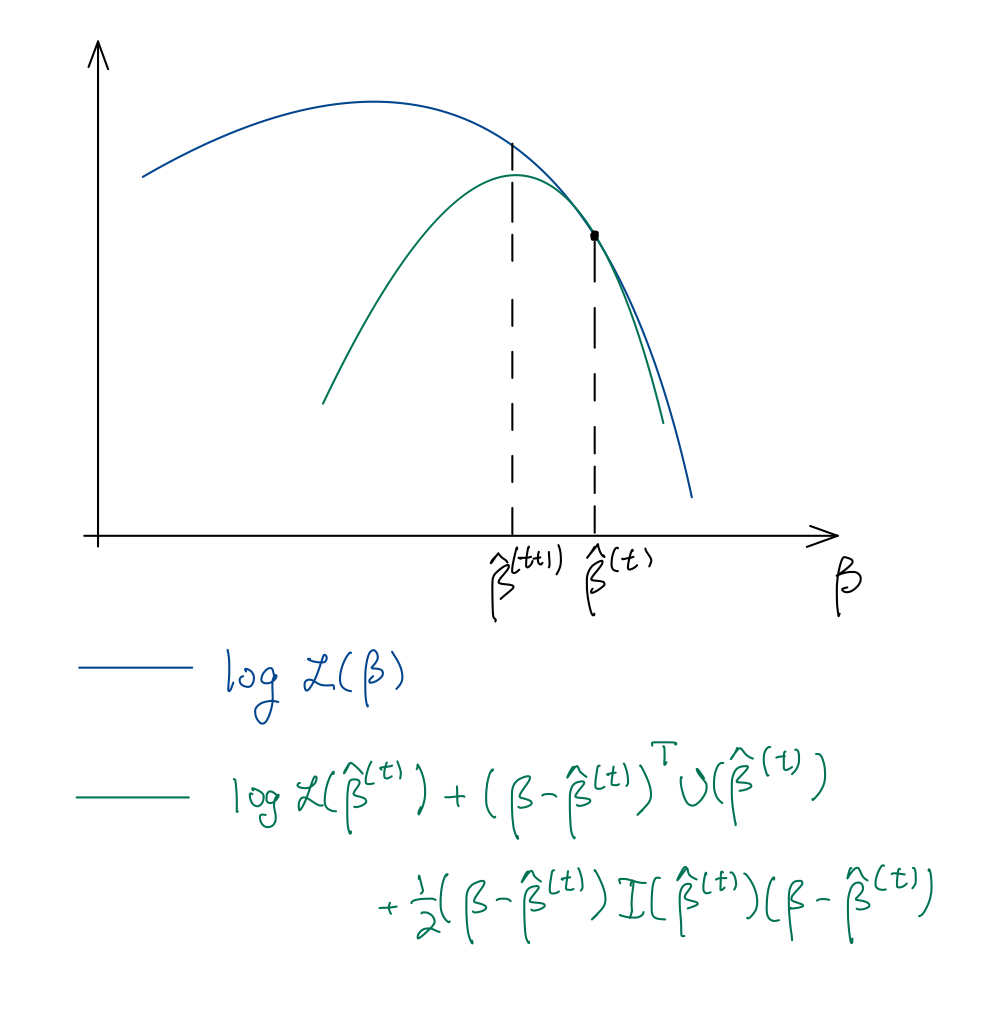
\includegraphics[width=0.6\textwidth,height=\textheight]{figures/newton-raphson.jpeg}

}

\caption{\label{fig-newton-raphson}Newton-Raphson iteratively
approximates the log likelihood via a quadratic function and maximizing
that function.}

\end{figure}

\hypertarget{sec-irls-interpretation}{%
\subsection{Iteratively reweighted least squares
(IRLS)}\label{sec-irls-interpretation}}

A nice interpretation of the Newton-Raphson algorithm is as a sequence
of weighted least squares fits, known as the iteratively reweighted
least squares (IRLS) algorithm. Suppose that we have a current estimate
\(\boldsymbol{\widehat \beta}^{(t)}\), and suppose we are looking for a
vector \(\boldsymbol{\beta}\) near \(\boldsymbol{\widehat \beta}^{(t)}\)
that fits the model even better. We have:

\[
\begin{split}
\mathbb{E}_{\boldsymbol{\beta}}[\boldsymbol{y}] &= g^{-1}(\boldsymbol{X} \boldsymbol{\beta}) \\
&\approx g^{-1}(\boldsymbol{X} \boldsymbol{\widehat \beta}^{(t)}) + \text{diag}(\partial \mu_i/\partial \eta_i)(\boldsymbol{X} \boldsymbol{\beta} - \boldsymbol{X} \boldsymbol{\widehat \beta}^{(t)}) \\
&= \boldsymbol{\widehat \mu}^{(t)} + (\boldsymbol{\widehat M}^{(t)})^{-1}(\boldsymbol{X} \boldsymbol{\beta} - \boldsymbol{X} \boldsymbol{\widehat \beta}^{(t)})
\end{split}
\]

and

\[
\text{Var}_{\boldsymbol{\beta}}[\boldsymbol{y}] \approx \phi_0 (\boldsymbol{\widehat W}^{(t)})^{-1}(\boldsymbol{\widehat M}^{(t)})^{-2} = \phi_0 \boldsymbol{\widehat W}^{(t)},
\]

recalling equation (\ref{eq-glm-variance-y}). Thus, up to the first two
moments, near \(\boldsymbol{\beta} = \boldsymbol{\widehat \beta}^{(t)}\)
the distribution of \(\boldsymbol{y}\) is approximately:

\[
\begin{aligned}
\boldsymbol{y} = \boldsymbol{\widehat \mu}^{(t)} + (\boldsymbol{\widehat M}^{(t)})^{-1}(\boldsymbol{X} \boldsymbol{\beta} - \boldsymbol{X} \boldsymbol{\widehat \beta}^{(t)}) + \boldsymbol{\epsilon}, \\
\boldsymbol{\epsilon} \sim N(\boldsymbol{0}, \phi_0 \boldsymbol{\widehat W}^{(t)}),
\end{aligned}
\]

or, equivalently:

\begin{equation}\protect\hypertarget{eq-second-order-approximation}{}{
\begin{aligned}
\boldsymbol{z}^{(t)} \equiv \boldsymbol{\widehat M}^{(t)}(\boldsymbol{y} - \boldsymbol{\widehat \mu}^{(t)}) + \boldsymbol{X} \boldsymbol{\widehat \beta}^{(t)} = \boldsymbol{X} \boldsymbol{\beta} + \boldsymbol{\epsilon}', \\
\boldsymbol{\epsilon}' \sim N(\boldsymbol{0}, \phi_0 (\boldsymbol{\widehat W}^{(t)})^{-1}).
\end{aligned}
}\label{eq-second-order-approximation}\end{equation}

The regression of the \emph{adjusted response variable}
\(\boldsymbol{z}^{(t)}\) on \(\boldsymbol{X}\) leaves us with a weighted
linear regression (hence the name \emph{working weights} for \(W_i\)),
whose maximum likelihood estimate is:

\begin{equation}\protect\hypertarget{eq-irls-iteration}{}{
\boldsymbol{\widehat \beta}^{(t+1)} = (\boldsymbol{X}^T \boldsymbol{\widehat W}^{(t)} \boldsymbol{X})^{-1} \boldsymbol{X}^T \boldsymbol{\widehat W}^{(t)} \boldsymbol{z}^{(t)},
}\label{eq-irls-iteration}\end{equation}

which we define as our next iterate. It's easy to verify that the IRLS
iteration (\ref{eq-irls-iteration}) is equivalent to the Newton-Raphson
iteration (\ref{eq-nr-iteration}). Note that we have derived these
algorithms for canonical links; they each can be derived for
non-canonical links but need not be equivalent in this more general
case.

\hypertarget{sec-glm-residuals}{%
\section{\texorpdfstring{Estimation of \(\phi_0\) and GLM
residuals}{Estimation of \textbackslash phi\_0 and GLM residuals}}\label{sec-glm-residuals}}

While sometimes the parameter \(\phi_0\) is known (e.g., for binomial or
Poisson GLMs), in other cases \(\phi_0\) must be estimated (e.g., for
the normal linear model). Recall from the linear model that we estimated
\(\sigma^2 = \phi_0\) by taking the sum of the squares of the residuals:
\(\widehat \sigma^2 = \frac{1}{n-p}\|\boldsymbol{y} - \boldsymbol{\widehat \mu}\|^2\).
However, it's unclear in the GLM context exactly how to define a
residual. In fact, there are two common ways of doing so, called
\emph{deviance residuals} and \emph{Pearson residuals}. Deviance
residuals are defined in terms of the unit deviance:

\[
  r^D_i \equiv \text{sign}(y_i - \widehat \mu_i)\sqrt{w_i d(y_i, \widehat \mu_i)}.
\]

On the other hand, Pearson residuals are defined as variance-normalized
residuals:

\[
  r^P_i \equiv \frac{y_i - \widehat \mu_i}{\sqrt{V(\widehat \mu_i)/w_i}}.
\]

These residuals can be viewed as residuals from the (converged) weighted
linear regression model (\ref{eq-second-order-approximation}). In the
normal case, these residuals coincide, but in the general case, they do
not. Based on these two notions of GLM residuals, we can define two
estimators of \(\phi_0\). One, based on the deviance residuals, is the
\emph{mean deviance estimator of dispersion}:

\[
\widetilde \phi^D_0 \equiv \frac{1}{n-p}\|r^D\|^2 \equiv \frac{1}{n-p}\sum_{i = 1}^n w_i d(y_i, \widehat \mu_i) \equiv \frac{1}{n-p}D(\boldsymbol{y}; \boldsymbol{\widehat \mu});
\]

recall that the total deviance
\(D(\boldsymbol{y}; \boldsymbol{\widehat \mu})\) is a generalization of
the residual sum of squares. The other, based on the Pearson residuals,
is called the \emph{Pearson estimator of dispersion}:

\begin{equation}\protect\hypertarget{eq-pearson-estimator-dispersion}{}{
\begin{split}
\widetilde \phi^P_0 &\equiv \frac{1}{n-p}X^2 \\
&\equiv \frac{1}{n-p}\|r^P\|^2 \\
&\equiv \frac{1}{n-p}\sum_{i = 1}^n w_i \frac{(y_i - \widehat \mu_i)^2}{V(\mu_i)}.
\end{split}
}\label{eq-pearson-estimator-dispersion}\end{equation}

\(X^2\) is known as the Pearson \(X^2\) statistic. The deviance-based
estimator can be more accurate than the Pearson estimator under
small-dispersion asymptotics. However, the Pearson estimator is more
robust when only the first two moments of the EDM model are correct and
in the absence of small-dispersion asymptotics. For these reasons, the
Pearson estimator is generally preferred.

\hypertarget{sec-glm-inf}{%
\chapter{Inference in GLMs}\label{sec-glm-inf}}

\hypertarget{sec-preliminaries}{%
\section{Preliminaries}\label{sec-preliminaries}}

\hypertarget{sec-inferential-goals}{%
\subsection{Inferential goals}\label{sec-inferential-goals}}

There are two types of inferential goals: hypothesis testing and
confidence interval/region construction.

\hypertarget{sec-hypothesis-testing}{%
\subsubsection{Hypothesis testing}\label{sec-hypothesis-testing}}

\begin{enumerate}
\def\labelenumi{\arabic{enumi}.}
\tightlist
\item
  \textbf{Single coefficient}: \(H_0: \beta_j = \beta_j^0\) versus
  \(H_1: \beta_j \neq \beta_j^0\) for some \(\beta_j^0 \in \mathbb{R}\).
\item
  \textbf{Group of coefficients}:
  \(H_0: \boldsymbol{\beta}_S = \boldsymbol{\beta}_S^0\) versus
  \(H_1: \boldsymbol{\beta}_S \neq \boldsymbol{\beta}_S^0\) for some
  \(S \subset \{0,\dots,p-1\}\) and some
  \(\boldsymbol{\beta}_S^0 \in \mathbb{R}^{|S|}\).
\item
  \textbf{Goodness of fit}: The goodness of fit null hypothesis is that
  the GLM (\ref{eq-glm-def}) is correctly specified. Consider the
  \emph{saturated model}:
  \begin{equation}\protect\hypertarget{eq-saturated-model}{}{
  y_i \overset{\text{ind}} \sim \text{EDM}(\mu_i, \phi_0/w_i) \quad \text{for} \quad i = 1,\dots,n.
  }\label{eq-saturated-model}\end{equation} Let \[
  \mathcal{M}^{\text{GLM}} \equiv \{\boldsymbol{\mu}: g(\mu_i) = \boldsymbol{x}_{i*}^T \boldsymbol{\beta} + o_i \text{ for some } \boldsymbol{\beta} \in \mathbb{R}^p\}
  \] be the set of mean vectors consistent with the GLM. Then, the
  goodness of fit testing problem is
  \(H_0: \boldsymbol{\mu} \in \mathcal{M}^{\text{GLM}}\) versus
  \(H_1: \boldsymbol{\mu} \notin \mathcal{M}^{\text{GLM}}\).
\end{enumerate}

\hypertarget{sec-confidence-interval-region}{%
\subsubsection{Confidence interval/region
construction}\label{sec-confidence-interval-region}}

\begin{enumerate}
\def\labelenumi{\arabic{enumi}.}
\tightlist
\item
  \textbf{Confidence interval for a single coefficient}: Here, the goal
  is to produce a confidence interval \(\text{CI}(\beta_j)\) for a
  coefficient \(\beta_j\).
\item
  \textbf{Confidence region for a group of coefficients}: Here, the goal
  is to produce a confidence region \(\text{CR}(\boldsymbol{\beta}_S)\)
  for a group of coefficients \(\boldsymbol{\beta}_S\).
\item
  \textbf{Confidence interval for a fitted value}: In GLMs, fitted
  values can either be considered for parameters on the linear scale
  (\(\eta_i = \boldsymbol{x}_{i*}^T \boldsymbol{\beta} + o_i\)) or the
  mean scale
  (\(\mu_i = g^{-1}(\boldsymbol{x}_{i*}^T \boldsymbol{\beta} + o_i)\)).
  The goal, then, is to produce confidence intervals
  \(\text{CI}(\eta_i)\) or \(\text{CI}(\mu_i)\) for \(\eta_i\) or
  \(\mu_i\), respectively.
\end{enumerate}

\hypertarget{sec-inferential-tools}{%
\subsection{Inferential tools}\label{sec-inferential-tools}}

Inference in GLMs is based on asymptotic likelihood theory. These
asymptotics can be based on \emph{large-sample asymptotics} or
\emph{small-dispersion asymptotics}. Large-sample asymptotics are
applicable for testing hypotheses and estimating parameters within
models where the number of parameters is fixed while the sample size
grows. Small-dispersion asymptotics are applicable for testing
hypotheses and estimating parameters within models where the dispersion
is small, regardless of the sample size. Large-sample asymptotics apply
to testing and estimating coefficients in GLMs (\ref{eq-glm-def}) with a
fixed number of parameters as the sample size grows, but not to testing
goodness of fit. Indeed, goodness-of-fit tests refer to the saturated
model (\ref{eq-saturated-model}), whose number of parameters grows with
\(n\). Small-dispersion asymptotics, on the other hand, apply to
goodness-of-fit testing.

Hypothesis tests (and, by inversion, confidence intervals) can be
constructed in three asymptotically equivalent ways: Wald tests,
likelihood ratio tests (LRT), and score tests. These tests can be
justified using either large-sample or small-dispersion asymptotics,
depending on the context. Despite their asymptotic equivalence, in
finite samples, some tests may be preferable to others (though for
normal linear models, these tests are equivalent in finite samples as
well). See Figure~\ref{fig-trinity-comparison}.

\begin{figure}

{\centering 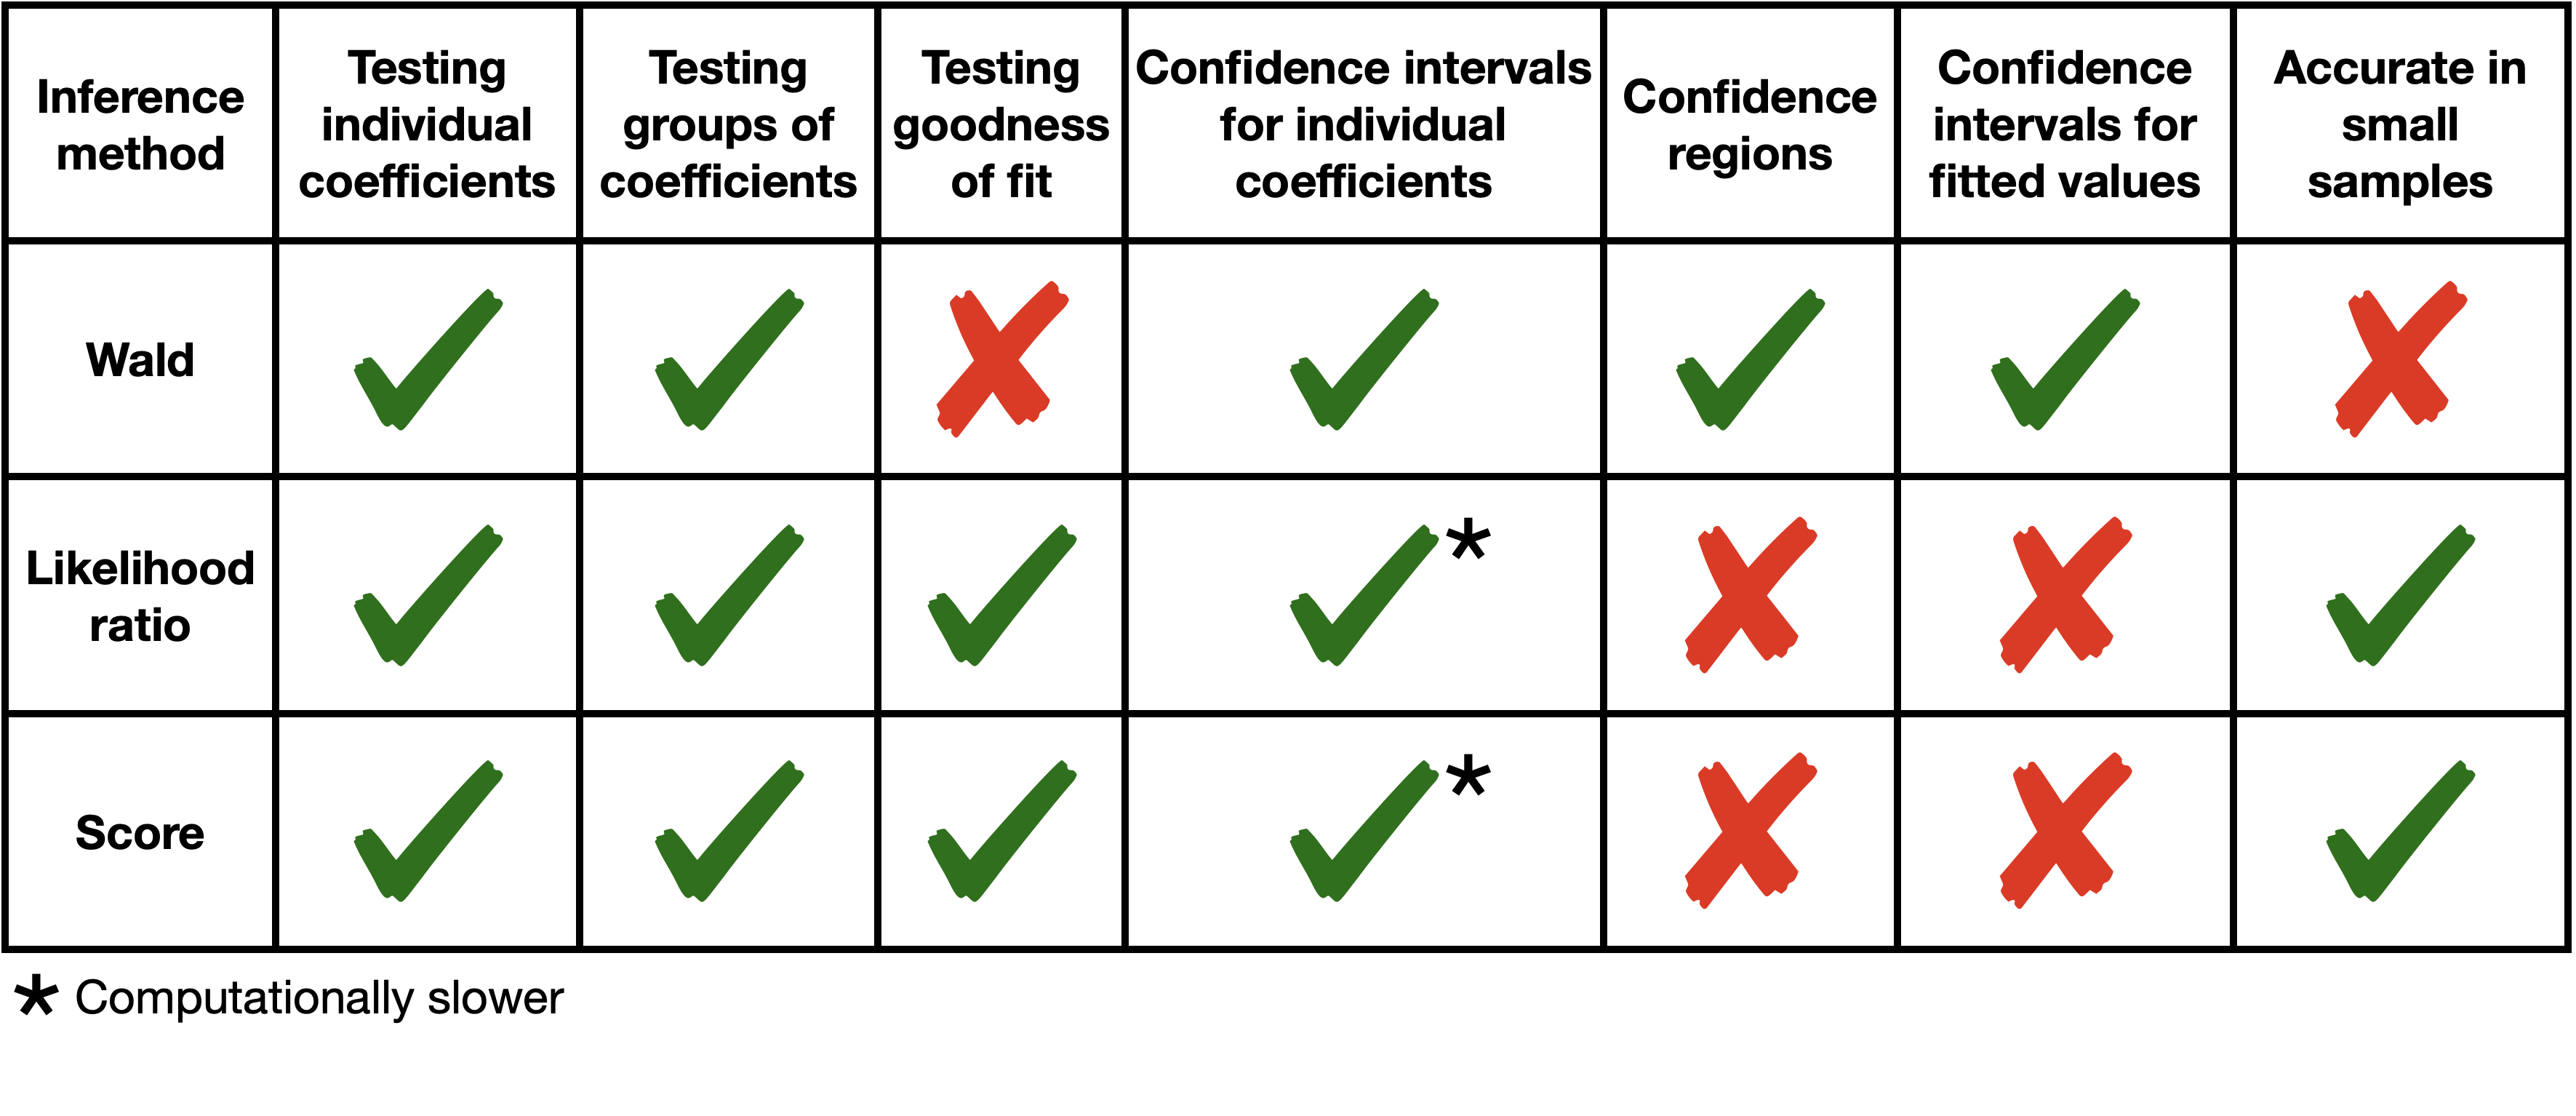
\includegraphics[width=1\textwidth,height=\textheight]{figures/trinity-comparison.png}

}

\caption{\label{fig-trinity-comparison}A comparison of the three
asymptotic methods for GLM inference.}

\end{figure}

\hypertarget{sec-wald-inference}{%
\section{Wald inference}\label{sec-wald-inference}}

Wald inference is based on the following asymptotic normality statement:

\begin{equation}\protect\hypertarget{eq-wald-approximation}{}{
\boldsymbol{\widehat \beta} \overset{\cdot}{\sim} N(\boldsymbol{\beta}, \boldsymbol{I}^{-1}(\boldsymbol{\beta})) = N(\boldsymbol{\beta}, \phi_0(\boldsymbol{X}^T \boldsymbol{W}(\boldsymbol{\beta}) \boldsymbol{X})^{-1}),
}\label{eq-wald-approximation}\end{equation}

recalling our derivation of the Fisher information from equation
(\ref{eq-glm-fisher-info}). This normal approximation can be justified
via the central limit theorem in the context of \emph{large-sample
asymptotics} or \emph{small-dispersion asymptotics}. Wald inference is
easy to carry out, and for this reason, it is considered the default
type of inference. However, as we will see in Unit 5, it also tends to
be the least accurate in small samples. Furthermore, Wald tests are
usually not applied for testing goodness of fit.

\hypertarget{sec-wald-test-single-coeff}{%
\subsection{\texorpdfstring{Wald test for \(\beta_j = \beta_j^0\) (known
\(\phi_0\))}{Wald test for \textbackslash beta\_j = \textbackslash beta\_j\^{}0 (known \textbackslash phi\_0)}}\label{sec-wald-test-single-coeff}}

Based on the Wald approximation (\ref{eq-wald-approximation}), under the
null hypothesis, we have:

\[
\begin{split}
\widehat \beta_j &\overset{\cdot}{\sim} N(\beta_j^0, \phi_0[(\boldsymbol{X}^T \boldsymbol{W}(\boldsymbol{\beta}) \boldsymbol{X})^{-1}]_{jj}) \\
&\approx N(\beta_j^0, \phi_0[(\boldsymbol{X}^T \boldsymbol{W}(\boldsymbol{\widehat \beta}) \boldsymbol{X})^{-1}]_{jj}) \\
&\equiv N(\beta_j^0, \text{SE}(\widehat \beta_j)^2),
\end{split}
\]

where we have used a plug-in estimator of the variance. This leads us to
the Wald \(z\)-test:

\[
\phi(\boldsymbol{X}, \boldsymbol{y}) \equiv 1\left(\left|\frac{\widehat \beta_j - \beta_j^0}{\text{SE}(\widehat \beta_j)}\right| > z_{1-\alpha/2}\right).
\]

Since a one-dimensional parameter is being tested, we can make the test
one-sided if desired.

\hypertarget{sec-wald-test-group-coeff}{%
\subsection{\texorpdfstring{Wald test for
\(\boldsymbol{\beta}_S = \boldsymbol{\beta}_S^0\) (known
\(\phi_0\))}{Wald test for \textbackslash boldsymbol\{\textbackslash beta\}\_S = \textbackslash boldsymbol\{\textbackslash beta\}\_S\^{}0 (known \textbackslash phi\_0)}}\label{sec-wald-test-group-coeff}}

Extending the reasoning above, we have under the null hypothesis that:

\[
\boldsymbol{\widehat \beta}_S \overset{\cdot}{\sim} N(\boldsymbol{\beta}_S^0, \phi_0[(\boldsymbol{X}^T \boldsymbol{W}(\boldsymbol{\beta}) \boldsymbol{X})^{-1}]_{S,S}) \approx N(\boldsymbol{\beta}_S^0, \phi_0[(\boldsymbol{X}^T \boldsymbol{W}(\boldsymbol{\widehat \beta}) \boldsymbol{X})^{-1}]_{S,S}),
\]

and therefore:

\[
\frac{1}{\phi_0} (\boldsymbol{\widehat \beta}_S - \boldsymbol{\beta}_S^0)^T \left([(\boldsymbol{X}^T \boldsymbol{W}(\boldsymbol{\widehat \beta}) \boldsymbol{X})^{-1}]_{S,S}\right)^{-1}(\boldsymbol{\widehat \beta}_S - \boldsymbol{\beta}_S^0) \overset{\cdot}{\sim} \chi^2_{|S|}.
\]

Hence, we have the Wald \(\chi^2\) test:

\[
\begin{split}
&\phi(\boldsymbol{X}, \boldsymbol{y}) \\
&\equiv 1\left(\frac{1}{\phi_0} (\boldsymbol{\widehat \beta}_S - \boldsymbol{\beta}_S^0)^T \left([(\boldsymbol{X}^T \boldsymbol{W}(\boldsymbol{\widehat \beta}) \boldsymbol{X})^{-1}]_{S,S}\right)^{-1}(\boldsymbol{\widehat \beta}_S - \boldsymbol{\beta}_S^0) > \chi^2_{|S|}(1-\alpha)\right).
\end{split}
\]

\hypertarget{sec-wald-ci-single-coeff}{%
\subsection{\texorpdfstring{Wald confidence interval for \(\beta_j\)
(known
\(\phi_0\))}{Wald confidence interval for \textbackslash beta\_j (known \textbackslash phi\_0)}}\label{sec-wald-ci-single-coeff}}

Inverting the Wald test for \(\beta_j\), we get a Wald confidence
interval:

\begin{equation}\protect\hypertarget{eq-conf-int-beta}{}{
\text{CI}(\beta_j) \equiv \widehat \beta_j \pm z_{1-\alpha/2} \cdot \text{SE}(\widehat \beta_j), 
}\label{eq-conf-int-beta}\end{equation} where \[
\text{SE}(\widehat \beta_j) \equiv \sqrt{\phi_0[(\boldsymbol{X}^T \boldsymbol{W}(\boldsymbol{\widehat \beta}) \boldsymbol{X})^{-1}]_{jj}}.
\]

\hypertarget{sec-wald-cr-group-coeff}{%
\subsection{\texorpdfstring{Wald confidence region for
\(\boldsymbol{\beta}_S\) (known
\(\phi_0\))}{Wald confidence region for \textbackslash boldsymbol\{\textbackslash beta\}\_S (known \textbackslash phi\_0)}}\label{sec-wald-cr-group-coeff}}

By inverting the test of
\(H_0: \boldsymbol{\beta}_S = \boldsymbol{\beta}_S^0\), we get the Wald
confidence region:

\[
\small
\begin{split}
\text{CR}(\boldsymbol{\beta}_S) \equiv \left\{\boldsymbol{\beta}_S: \frac{1}{\phi_0} (\boldsymbol{\widehat \beta}_S - \boldsymbol{\beta}_S)^T \left([(\boldsymbol{X}^T \boldsymbol{W}(\boldsymbol{\widehat \beta}) \boldsymbol{X})^{-1}]_{S,S}\right)^{-1}(\boldsymbol{\widehat \beta}_S - \boldsymbol{\beta}_S) \leq \chi^2_{|S|}(1-\alpha)\right\}.
\end{split}
\]

If \(S = \{0, 1, \dots, p-1\}\), we are left with:

\[
\text{CR}(\boldsymbol{\beta}_S) \equiv \left\{\boldsymbol{\beta}: \frac{1}{\phi_0} (\boldsymbol{\widehat \beta} - \boldsymbol{\beta})^T \boldsymbol{X}^T \boldsymbol{W}(\boldsymbol{\widehat \beta}) \boldsymbol{X} (\boldsymbol{\widehat \beta} - \boldsymbol{\beta}) \leq \chi^2_{p}(1-\alpha)\right\}.
\]

\hypertarget{sec-wald-ci-fitted-values}{%
\subsection{\texorpdfstring{Wald confidence intervals for \(\eta_i\) and
\(\mu_i\) (known
\(\phi_0\))}{Wald confidence intervals for \textbackslash eta\_i and \textbackslash mu\_i (known \textbackslash phi\_0)}}\label{sec-wald-ci-fitted-values}}

Given the Wald approximation (\ref{eq-wald-approximation}), we have:

\[
\widehat \eta_i \equiv o_i + \boldsymbol{x}_{i*}^T \boldsymbol{\widehat \beta} \overset{\cdot}{\sim} N(\eta_i, \phi_0 \cdot \boldsymbol{x}_{i*}^T (\boldsymbol{X}^T \boldsymbol{W}(\boldsymbol{\widehat \beta}) \boldsymbol{X})^{-1} \boldsymbol{x}_{i*}) \equiv N(\eta_i, \text{SE}(\hat \eta_i)^2).
\]

Hence, the Wald interval for \(\eta_i\) is:

\[
\text{CI}(\eta_i) \equiv o_i + \boldsymbol{x}_{i*}^T \boldsymbol{\widehat\beta} \pm z_{1-\alpha/2} \cdot \text{SE}(\hat \eta_i),
\] where \[
\text{SE}(\hat \eta_i) \equiv \sqrt{\phi_0 \boldsymbol{x}_{i*}^T (\boldsymbol{X}^T \boldsymbol{W}(\boldsymbol{\widehat \beta}) \boldsymbol{X})^{-1} \boldsymbol{x}_{i*}}.
\]

A confidence interval for
\(\mu_i \equiv \mathbb{E}_{\boldsymbol{\beta}}[y_i] = g^{-1}(\eta_i)\)
can be obtained by applying the monotonic function \(g^{-1}\) to the
endpoints of the confidence interval for \(\eta_i\). Note that the
resulting confidence interval may be asymmetric. We can get a symmetric
interval by applying the delta method, but this interval would be less
accurate because it involves the delta method approximation in addition
to the Wald approximation.

\hypertarget{sec-wald-inference-unknown-dispersion}{%
\subsection{\texorpdfstring{Wald inference when \(\phi_0\) is
unknown}{Wald inference when \textbackslash phi\_0 is unknown}}\label{sec-wald-inference-unknown-dispersion}}

When \(\phi_0\) is unknown, we need to plug in an estimate
\(\widetilde \phi_0\) (e.g.~the deviance-based or Pearson-based
estimate). Now our standard errors are \[
\text{SE}(\widehat \beta_j) \equiv \sqrt{\widetilde \phi_0 \cdot [(\boldsymbol{X}^T \boldsymbol{W}(\boldsymbol{\widehat \beta}) \boldsymbol{X})^{-1}]_{jj}},
\] and our test statistic for \(H_0: \beta_j = \beta_j^0\) is \[
\frac{\widehat \beta_j - \beta_j^0}{\sqrt{\widetilde \phi_0}\sqrt{[(\boldsymbol{X}^T \boldsymbol{W}(\boldsymbol{\widehat \beta}) \boldsymbol{X})^{-1}]_{jj}}}.
\]

Unlike linear regression, it is not the case in general that
\(\boldsymbol{\widehat \beta}\) and \(\widetilde \phi_0\) are
independent. Nevertheless, they are \emph{asymptotically independent}.
Therefore, the above statistic is \emph{approximately} distributed as
\(t_{n-p}\). Hence, the test for \(H_0: \beta_j = \beta_j^0\) is:

\[
\phi(\boldsymbol{X}, \boldsymbol{y}) \equiv 1\left(\left|\frac{\widehat \beta_j - \beta_j^0}{\text{SE}(\widehat \beta_j)}\right| > t_{n-p}(1-\alpha/2)\right).
\]

Likewise, we would replace \(z_{1-\alpha}\) by \(t_{n-p}(1-\alpha/2)\)
for all tests and confidence intervals concerning univariate quantities.
For multivariate quantities, we will get approximate \(F\) distributions
instead of approximate \(\chi^2\) distributions. For example:

\[
\frac{\frac{1}{|S|}(\boldsymbol{\widehat \beta}_S - \boldsymbol{\beta}_S^0)^T \left([(\boldsymbol{X}^T \boldsymbol{W}(\boldsymbol{\widehat \beta}) \boldsymbol{X})^{-1}]_{S,S}\right)^{-1}(\boldsymbol{\widehat \beta}_S - \boldsymbol{\beta}_S^0)}{\widetilde \phi_0} \overset{\cdot}{\sim} F_{|S|, n-p}.
\]

\hypertarget{sec-likelihood-ratio-inference}{%
\section{Likelihood ratio
inference}\label{sec-likelihood-ratio-inference}}

\hypertarget{sec-likelihood-ratio-coeff-known}{%
\subsection{\texorpdfstring{Testing one or more coefficients (\(\phi_0\)
known)}{Testing one or more coefficients (\textbackslash phi\_0 known)}}\label{sec-likelihood-ratio-coeff-known}}

Let
\(\ell(\boldsymbol{y}, \boldsymbol{\mu}) = -\frac{D(\boldsymbol{y}, \boldsymbol{\mu})}{2\phi_0} + C\)
be the GLM log-likelihood (recall equation
(\ref{eq-glm-likelihood-via-deviance})). Let
\(H_0: \boldsymbol{\beta}_S = \boldsymbol{\beta}_S^0\) be a null
hypothesis about some subset of variables
\(S \subset \{0, 1, \dots, p-1\}\), and let
\(\boldsymbol{\widehat{\mu}}_{\text{-}S}\) be the maximum likelihood
estimate under the null hypothesis. Likelihood ratio inference is based
on the following asymptotic chi-square distribution:

\begin{equation}\protect\hypertarget{eq-likelihood-ratio-approximation}{}{
2(\ell(\boldsymbol{y}, \boldsymbol{\widehat{\mu}}) - \ell(\boldsymbol{y}, \boldsymbol{\widehat{\mu}}_{\text{-}S})) = \frac{D(\boldsymbol{y}, \boldsymbol{\widehat{\mu}}_{\text{-}S}) - D(\boldsymbol{y}, \boldsymbol{\widehat{\mu}})}{\phi_0} \overset{\cdot}{\sim} \chi^2_{|S|}.
}\label{eq-likelihood-ratio-approximation}\end{equation}

This approximation holds either in large samples (large-sample
asymptotics) or in small samples but with small dispersion
(small-dispersion asymptotics). The latter has to do with the fact that
under small-dispersion asymptotics,

\[
\frac{d(y_i, \mu_i)}{\phi_0/w_i} \overset{\cdot}{\sim} \chi^2_1,
\]

so

\[
\frac{D(\boldsymbol{y}, \boldsymbol{\mu})}{\phi_0} = \sum_{i = 1}^n \frac{d(y_i, \mu_i)}{\phi_0/w_i} \overset{\cdot}{\sim} \chi^2_n.
\]

Suppose we wish to test the null hypothesis
\(H_0: \boldsymbol{\beta}_S = \boldsymbol{\beta}_S^0\). Then, based on
the approximation (\ref{eq-likelihood-ratio-approximation}), we can
define the likelihood ratio test:

\[
\phi(\boldsymbol{X}, \boldsymbol{y}) \equiv 1\left(\frac{D(\boldsymbol{y}, \boldsymbol{\widehat{\mu}}_{\text{-}S}) - D(\boldsymbol{y}, \boldsymbol{\widehat{\mu}})}{\phi_0} > \chi^2_{|S|}(1-\alpha)\right).
\]

\hypertarget{sec-likelihood-ratio-ci-single-coeff}{%
\subsection{Confidence interval for a single
coefficient}\label{sec-likelihood-ratio-ci-single-coeff}}

We can obtain a confidence interval for \(\beta_j\) by inverting the
likelihood ratio test. Let
\(\boldsymbol{\widehat{\mu}}_{\text{-}j}(\beta_j^0)\) be the fitted mean
vector under the constraint \(\beta_j = \beta_j^0\). Then, inverting the
likelihood ratio test gives us the confidence interval:

\[
\text{CI}(\beta_j) \equiv \left\{\beta_j: \frac{D(\boldsymbol{y}, \boldsymbol{\widehat{\mu}}_{\text{-}j}(\beta_j)) - D(\boldsymbol{y}, \boldsymbol{\widehat{\mu}})}{\phi_0} \leq \chi^2_{|S|}(1-\alpha)\right\}.
\]

Likelihood ratio-based confidence intervals tend to be more accurate
than Wald intervals, especially when the parameter is near the edge of
the parameter space, but they require more computation because
\(\boldsymbol{\widehat{\mu}}_{\text{-}j}(\beta_j)\) must be computed on
a large grid of \(\beta_j\) values. If we wanted to create
\emph{confidence regions} for groups of parameters, this would become
computationally intensive due to the curse of dimensionality.

\hypertarget{sec-likelihood-ratio-goodness-of-fit}{%
\subsection{\texorpdfstring{Goodness of fit testing (\(\phi_0\)
known)}{Goodness of fit testing (\textbackslash phi\_0 known)}}\label{sec-likelihood-ratio-goodness-of-fit}}

For \(\phi_0\) known, we can also construct a goodness of fit test. To
this end, we compare the deviances of the GLM and saturated model:

\[
\frac{D(\boldsymbol{y}, \boldsymbol{\widehat{\mu}}) - D(\boldsymbol{y}, \boldsymbol{y})}{\phi_0} = \frac{D(\boldsymbol{y}; \boldsymbol{\widehat{\mu}})}{\phi_0} \overset{\cdot}{\sim} \chi^2_{n-p}.
\]

Note that the goodness of fit test is a significance test with respect
to the saturated model (\ref{eq-saturated-model}), which has \(n\) free
parameters. Therefore, the number of free parameters increases with the
sample size, so large-sample asymptotics cannot justify this test.
Instead, we must rely on small-dispersion asymptotics. In particular,
the likelihood ratio test relies on the saddlepoint approximation for
small dispersions. To verify whether the saddlepoint approximation is
accurate, we can apply the rules of thumb from
Section~\ref{sec-saddlepoint-approximation-accuracy} for each
observation \(y_i\), when it is drawn from the distribution fitted under
the GLM (rather than the saturated model). For instance, we can check
that \(m \hat \mu_i \geq 3\) and \(m(1-\hat \mu_i) \geq 3\) in the case
of grouped logistic regression of \(\hat \mu_i \geq 3\) for Poisson
regression. Here, \(\hat \mu_i\) are the fitted means under the GLM.

\hypertarget{sec-likelihood-ratio-unknown-dispersion}{%
\subsection{\texorpdfstring{Likelihood ratio inference for \(\phi_0\)
unknown}{Likelihood ratio inference for \textbackslash phi\_0 unknown}}\label{sec-likelihood-ratio-unknown-dispersion}}

If \(\phi_0\) is unknown, we can estimate it as discussed above and
construct an \(F\)-statistic as follows:

\[
F \equiv \frac{(D(\boldsymbol{y}; \boldsymbol{\widehat{\mu}}_{\text{-}S}) - D(\boldsymbol{y}; \boldsymbol{\widehat{\mu}}))/|S|}{\widetilde{\phi}_0}.
\]

In normal linear model theory, the null distribution of \(F\) is
\emph{exactly} \(F_{|S|, n-p}\). For GLMs, the null distribution of
\(F\) is \emph{approximately} \(F_{|S|, n-p}\). We can use this \(F\)
distribution to construct hypothesis tests for groups of coefficients,
or invert it to get a confidence interval for a single coefficient. We
cannot construct a goodness of fit test in the case that \(\phi_0\) is
unknown because the residual degrees of freedom would be used up to
estimate \(\phi_0\) rather than to carry out inference.

\hypertarget{sec-score-inference}{%
\section{Score-based inference}\label{sec-score-inference}}

Score-based inference can be used for the same set of inferential tasks
as likelihood ratio inference.

\hypertarget{sec-score-test-multiple-coeff}{%
\subsection{\texorpdfstring{Testing multiple coefficients (\(\phi_0\)
known)}{Testing multiple coefficients (\textbackslash phi\_0 known)}}\label{sec-score-test-multiple-coeff}}

Let \(H_0: \boldsymbol{\beta}_S = \boldsymbol{\beta}_S^0\) be a null
hypothesis about a subset of variables \(S\), and let
\(\boldsymbol{\widehat{\beta}}^0\) be the maximum likelihood estimate
under this null hypothesis. In particular, let
\(\boldsymbol{\widehat{\beta}}^0_S \equiv \boldsymbol{\beta}_S^0\) and
\begin{equation}\protect\hypertarget{eq-score-null-estimate}{}{
\boldsymbol{\widehat{\beta}}^0_{\text{-}S} = \underset{\boldsymbol{\beta}_{\text{-}S}}{\arg \max}\ \ell(\boldsymbol{\beta}^0_{S}, \boldsymbol{\beta}_{\text{-}S}).
}\label{eq-score-null-estimate}\end{equation} Let us partition the score
vector
\(\boldsymbol U(\boldsymbol{\beta}) = \frac{\partial \ell(\boldsymbol{\beta})}{\partial \boldsymbol{\beta}} \equiv (\boldsymbol U_S(\boldsymbol \beta), \boldsymbol U_{\text{-}S}(\boldsymbol \beta))\).
We have
\begin{equation}\protect\hypertarget{eq-glm-score-distribution}{}{
\begin{split}
\boldsymbol U(\boldsymbol \beta) &= { \boldsymbol U_S(\boldsymbol \beta) \choose \boldsymbol U_{\text{-}S}(\boldsymbol \beta) } \\
&\sim N\left(0, \boldsymbol I(\boldsymbol \beta)\right) = N\left(0, \begin{bmatrix} \boldsymbol I_{S,S}(\boldsymbol \beta) & \boldsymbol I_{S,\text{-}S}(\boldsymbol \beta) \\ \boldsymbol I_{\text{-}S,S}(\boldsymbol \beta) & \boldsymbol I_{\text{-}S,\text{-}S}(\boldsymbol \beta) \end{bmatrix}\right).
\end{split}
}\label{eq-glm-score-distribution}\end{equation} This approximation can
be justified either by small-dispersion asymptotics or large-sample
asymptotics (both based on the central limit theorem). The score test
statistic is based on plugging in the null estimate
\(\boldsymbol{\widehat{\beta}}^0\) into the score vector and extracting
the components corresponding to \(S\): \[
\boldsymbol U_S(\boldsymbol{\widehat{\beta}}^0).
\] This vector does not have the distribution obtained from the
coordinates \(S\) of equation (\ref{eq-glm-score-distribution}) because
an estimate is plugged in. Instead, we can derive the distribution of
this vector by conditioning on
\(\boldsymbol U_{\text{-}S}(\boldsymbol{\widehat{\beta}}^0) = 0\):
\begin{equation}\protect\hypertarget{eq-conditioning-score-test}{}{
\begin{split}
\boldsymbol U_S(\boldsymbol{\widehat{\beta}}^0) &\overset d \approx \left.\mathcal L(\boldsymbol U_S(\boldsymbol \beta) \mid \boldsymbol U_{\text{-}S}(\boldsymbol \beta) = 0)\right|_{\boldsymbol \beta = \boldsymbol{\widehat{\beta}}^0} \\
& \overset \cdot \sim N\left(0, \boldsymbol I_{S,S}(\boldsymbol{\widehat{\beta}}^0) - \boldsymbol I_{S, \text{-}S}(\boldsymbol{\widehat{\beta}}^0)\boldsymbol I_{\text{-}S, \text{-}S}(\boldsymbol{\widehat{\beta}}^0)^{-1}\boldsymbol I_{\text{-}S, S}(\boldsymbol{\widehat{\beta}}^0)\right).
\end{split}
}\label{eq-conditioning-score-test}\end{equation} The second line is
obtained from (\ref{eq-glm-score-distribution}) using the formula for a
conditional distribution of a multivariate normal distribution.
Therefore, the score test is based on the following chi-square
approximation: \[
\boldsymbol U_S(\boldsymbol{\widehat{\beta}}^0)^T \left[\boldsymbol I_{S,S}(\boldsymbol{\widehat{\beta}}^0) - \boldsymbol I_{S, \text{-}S}(\boldsymbol{\widehat{\beta}}^0)\boldsymbol I_{\text{-}S, \text{-}S}(\boldsymbol{\widehat{\beta}}^0)^{-1}\boldsymbol I_{\text{-}S, S}(\boldsymbol{\widehat{\beta}}^0)\right]^{-1} \boldsymbol U_S(\boldsymbol{\widehat{\beta}}^0) \overset \cdot \sim \chi^2_{|S|}.
\] Recalling the expressions for the score (\ref{eq-glm-score}) and
Fisher information matrix (\ref{eq-glm-fisher-info}) in GLMs, we derive
the score statistic \[
\begin{split}
&T^2_{\text{score}}(\boldsymbol X, \boldsymbol y) \equiv \\
&\frac{1}{\phi_0}(\boldsymbol{y} - \boldsymbol{\widehat{\mu}}^0)^T \boldsymbol{\widehat{W}}^0 \boldsymbol{\widehat{M}}^0 \boldsymbol{X}_{*,S} \times \\
& \quad \left[\boldsymbol X_{*,S}^T \boldsymbol {\widehat W}^{0}\boldsymbol X_{*,S} - \boldsymbol X_{*,S}^T \boldsymbol {\widehat W}^{0}\boldsymbol X_{*,\text{-}S}(\boldsymbol X_{*,\text{-}S}^T \boldsymbol {\widehat W}^{0}\boldsymbol X_{*,\text{-}S})^{-1}\boldsymbol X_{*,\text{-}S}^T \boldsymbol {\widehat W}^{0}\boldsymbol X_{*,S} \right]^{-1} \times \\
& \quad \boldsymbol{X}_{*,S}^T \boldsymbol{\widehat{M}}^0 \boldsymbol{\widehat{W}}^0 (\boldsymbol{y} - \boldsymbol{\widehat{\mu}}^0).
\end{split}
\] The score test is therefore \[
\phi(\boldsymbol X, \boldsymbol y) \equiv 1(T^2_{\text{score}}(\boldsymbol X, \boldsymbol y) > \chi^2_{|S|}(1-\alpha)).
\] An equivalent formulation of the score test can be derived by noting
that \[
\left[I_{S,S}(\boldsymbol{\widehat{\beta}}^0) - \boldsymbol I_{S, \text{-}S}(\boldsymbol{\widehat{\beta}}^0)\boldsymbol I_{\text{-}S, \text{-}S}(\boldsymbol{\widehat{\beta}}^0)^{-1}\boldsymbol I_{\text{-}S, S}(\boldsymbol{\widehat{\beta}}^0)\right]^{-1} = [\boldsymbol I(\boldsymbol{\widehat{\beta}}^0)^{-1}]_{S,S}.
\] Hence, we have \[
\begin{split}
&\boldsymbol U_S(\boldsymbol{\widehat{\beta}}^0)^T \left[\boldsymbol I_{S,S}(\boldsymbol{\widehat{\beta}}^0) - \boldsymbol I_{S, \text{-}S}(\boldsymbol{\widehat{\beta}}^0)\boldsymbol I_{\text{-}S, \text{-}S}(\boldsymbol{\widehat{\beta}}^0)^{-1}\boldsymbol I_{\text{-}S, S}(\boldsymbol{\widehat{\beta}}^0)\right]^{-1} \boldsymbol U_S(\boldsymbol{\widehat{\beta}}^0) \\
&\quad= \boldsymbol U_S(\boldsymbol{\widehat{\beta}}^0)^T [\boldsymbol I(\boldsymbol{\widehat{\beta}}^0)^{-1}]_{S,S} \boldsymbol U_S(\boldsymbol{\widehat{\beta}}^0) \\
&\quad= \boldsymbol U(\boldsymbol{\widehat{\beta}}^0)^T \boldsymbol I(\boldsymbol{\widehat{\beta}}^0)^{-1} \boldsymbol U(\boldsymbol{\widehat{\beta}}^0),
\end{split}
\] where the last step used the fact that
\(\boldsymbol U_{\text{-}S}(\boldsymbol{\widehat \beta}^{0}) = 0\).
Specializing to GLMs, we find that the score test statistic can be
written as
\begin{equation}\protect\hypertarget{eq-score-stat-alternative}{}{
\begin{split}
&T^2_{\text{score}}(\boldsymbol X, \boldsymbol y) = \\
&\frac{1}{\phi_0} (\boldsymbol y - \boldsymbol{\widehat \mu}^0) \boldsymbol{\widehat W}^0 \boldsymbol{\widehat M}^0 \boldsymbol X (\boldsymbol X^T \boldsymbol{\widehat W}^0 \boldsymbol X)^{-1} \boldsymbol X^T \boldsymbol{\widehat M}^0 \boldsymbol{\widehat W}^0 (\boldsymbol y - \boldsymbol{\widehat \mu}^0).
\end{split}
}\label{eq-score-stat-alternative}\end{equation}

\hypertarget{sec-score-test-single-coeff}{%
\subsection{\texorpdfstring{Testing a single coefficient (\(\phi_0\)
known)}{Testing a single coefficient (\textbackslash phi\_0 known)}}\label{sec-score-test-single-coeff}}

If \(S = \{j\}\), the normal approximation
(\ref{eq-conditioning-score-test}) specializes to \[
T_{\text{score}} \overset{\cdot}{\sim} N(0, 1),
\] where \[
\begin{split}
&T_{\text{score}} = \\
&\frac{\boldsymbol{x}_{*,j}^T \boldsymbol{\widehat{M}}^0 \boldsymbol{\widehat{W}}^0 (\boldsymbol{y} - \boldsymbol{\widehat{\mu}}^0)}{\sqrt{\phi_0 (\boldsymbol x_{*,j}^T \boldsymbol {\widehat W}^{0}\boldsymbol x_{*,j} - \boldsymbol x_{*,j}^T \boldsymbol {\widehat W}^{0}\boldsymbol X_{*,\text{-}j}(\boldsymbol X_{*,\text{-}j}^T \boldsymbol {\widehat W}^{0}\boldsymbol X_{*,\text{-}j})^{-1}\boldsymbol X_{*,\text{-}j}^T \boldsymbol {\widehat W}^{0}\boldsymbol x_{*,j})}}.
\end{split}
\]

Unlike its multivariate counterparts, we can construct not just a
two-sided test but also one-sided tests based on this normal
approximation. For example, below is a right-sided score test for
\(H_0: \beta_j = \beta_j^0\):

\[
\phi(\boldsymbol{X}, \boldsymbol{y}) = 1\left(T_{\text{score}} > z_{1-\alpha}\right).
\]

The nice thing about the score test is that the model need only be fit
under the null hypothesis. Therefore, computation can be recycled if
\(\boldsymbol X_{*, \text{-}j}\) is a standard set of control variables
and there are several options for \(\boldsymbol x_{*, j}\) to test.

\hypertarget{sec-score-ci-single-coeff}{%
\subsection{\texorpdfstring{Confidence interval for a single coefficient
(\(\phi_0\)
known)}{Confidence interval for a single coefficient (\textbackslash phi\_0 known)}}\label{sec-score-ci-single-coeff}}

Just as with the likelihood ratio test, it is possible to invert a score
test for a single coefficient to obtain a confidence interval. It is
uncommon to invert a multivariate test to obtain a confidence region for
multiple coordinates of \(\boldsymbol{\beta}\), given the
computationally expensive search across a grid of possible
\(\boldsymbol{\beta}\) values.

\hypertarget{sec-score-goodness-of-fit}{%
\subsection{\texorpdfstring{Goodness of fit testing (\(\phi_0\)
known)}{Goodness of fit testing (\textbackslash phi\_0 known)}}\label{sec-score-goodness-of-fit}}

We can view goodness of fit testing as testing a hypothesis about the
coefficients in the following augmented GLM: \[
y_i \sim \text{EDM}(\mu_i, \phi_i); \quad g(\mu_i) = \boldsymbol x_{i*}^T \boldsymbol \beta + \boldsymbol z_{i*}^T \boldsymbol \gamma, 
\] where \(\boldsymbol Z \in \mathbb R^{n \times (n-p)}\) is a matrix of
extra variables so that the columns of the augmented model matrix
\(\widetilde{\boldsymbol X} \equiv [\boldsymbol X, \boldsymbol Z]\) form
a basis for \(\mathbb R^n\). Then, the goodness of fit null hypothesis
is \(H_0: \boldsymbol \gamma = \boldsymbol 0\), and the alternative
hypothesis is the saturated model. To test this hypothesis, we use the
score test statistic in the form of equation
(\ref{eq-score-stat-alternative}) with the augmented model matrix
\(\widetilde{\boldsymbol X}\) in place of \(\boldsymbol X\) and the GLM
fits
\(\boldsymbol {\widehat \mu}, \boldsymbol{\widehat W}, \boldsymbol{\widehat M}\)
in place of
\(\boldsymbol{\widehat \mu}^0, \boldsymbol{\widehat W}^0, \boldsymbol{\widehat M}^0\)
to reflect that the full original GLM is being fit under the null
hypothesis. Therefore, we get the score statistic \[
T^2_{\text{score}} = \frac{1}{\phi_0} (\boldsymbol y - \boldsymbol{\widehat \mu}) \boldsymbol{\widehat W} \boldsymbol{\widehat M} \widetilde{\boldsymbol X} (\widetilde{\boldsymbol X}^T \boldsymbol{\widehat W} \widetilde{\boldsymbol X})^{-1} \widetilde{\boldsymbol X}^T \boldsymbol{\widehat M} \boldsymbol{\widehat W} (\boldsymbol y - \boldsymbol{\widehat \mu}).
\] Now, note that the matrix \(\widetilde{\boldsymbol X}\) is a
full-rank square matrix, and therefore it is invertible. Hence, we can
simplify the statistic as follows: \[
\begin{split}
T^2_{\text{score}} &= \frac{1}{\phi_0} (\boldsymbol y - \boldsymbol{\widehat \mu}) \boldsymbol{\widehat W} \boldsymbol{\widehat M} \widetilde{\boldsymbol X} \widetilde{\boldsymbol X}^{-1} \boldsymbol{\widehat W}^{-1}((\widetilde{\boldsymbol X})^{T})^{-1} \widetilde{\boldsymbol X}^T \boldsymbol{\widehat M} \boldsymbol{\widehat W} (\boldsymbol y - \boldsymbol{\widehat \mu}) \\
&= \frac{1}{\phi_0} (\boldsymbol y - \boldsymbol{\widehat \mu}) \boldsymbol{\widehat W} \boldsymbol{\widehat M} \boldsymbol{\widehat W}^{-1} \boldsymbol{\widehat M} \boldsymbol{\widehat W} (\boldsymbol y - \boldsymbol{\widehat \mu}) \\
&= \frac{1}{\phi_0}(\boldsymbol{y} - \boldsymbol{\widehat{\mu}})^T \boldsymbol{\widehat{W}} \boldsymbol{\widehat{M}}^2 (\boldsymbol{y} - \boldsymbol{\widehat{\mu}}) \\
&= \frac{1}{\phi_0}(\boldsymbol{y} - \boldsymbol{\widehat{\mu}})^T \text{diag}\left( \frac{w_i}{V(\widehat{\mu}_i)} \right) (\boldsymbol{y} - \boldsymbol{\widehat{\mu}}) \\
&= \frac{1}{\phi_0}\sum_{i=1}^n \frac{w_i (y_i - \widehat{\mu}_i)^2}{V(\widehat{\mu}_i)} \\
&\equiv \frac{1}{\phi_0} X^2,
\end{split}
\] where \(X^2\) is the Pearson chi-square statistic. Therefore, the
score test for goodness of fit is:

\[
\phi(\boldsymbol{X}, \boldsymbol{y}) \equiv 1\left(X^2 > \phi_0 \chi^2_{n-p}(1-\alpha)\right).
\]

In the context of contingency table analysis (see the next chapter),
this test reduces to the Pearson chi-square test of independence between
two categorical variables. This test was proposed in 1900; it was only
pointed out about a century later that this is a score test (Smyth
2003).

As with the likelihood ratio test for goodness of fit, the score test
for goodness of fit must be justified by small-dispersion asymptotics.
In particular, the score test for goodness of fit relies on the central
limit theorem for small dispersions. To verify whether this
approximation is accurate, we can apply the rules of thumb from
Section~\ref{sec-normal-approx-accuracy} for each observation \(y_i\),
when it is drawn from the distribution fitted under the GLM (rather than
the saturated model). For instance, we can check that
\(m \hat \mu_i \geq 5\) and \(m(1-\hat \mu_i) \geq 5\) in the case of
grouped logistic regression of \(\hat \mu_i \geq 5\) for Poisson
regression. Here, \(\hat \mu_i\) are the fitted means under the GLM.

\hypertarget{sec-score-test-unknown-dispersion}{%
\subsection{\texorpdfstring{Score test inference for \(\phi_0\)
unknown}{Score test inference for \textbackslash phi\_0 unknown}}\label{sec-score-test-unknown-dispersion}}

Score test inference for one or more coefficients
\(\boldsymbol{\beta}_S\) can be achieved by replacing \(\phi_0\) with
one of its estimators and replacing the normal and chi-square
distributions with \(t\) and \(F\) distributions, respectively. For
example, the score test for a single coefficient \(\beta_j\) is:

\[
\phi(\boldsymbol{X}, \boldsymbol{y}) = 1\left(T_{\text{score}} > t_{n-p}(1-\alpha)\right),
\] where \[
\begin{split}
&T_{\text{score}} = \\
&\frac{\boldsymbol{x}_{*,j}^T \boldsymbol{\widehat{M}}^0 \boldsymbol{\widehat{W}}^0 (\boldsymbol{y} - \boldsymbol{\widehat{\mu}}^0)}{\sqrt{\tilde \phi_0 (\boldsymbol x_{*,j}^T \boldsymbol {\widehat W}^{0}\boldsymbol x_{*,j} - \boldsymbol x_{*,j}^T \boldsymbol {\widehat W}^{0}\boldsymbol X_{*,\text{-}j}(\boldsymbol X_{*,\text{-}j}^T \boldsymbol {\widehat W}^{0}\boldsymbol X_{*,\text{-}j})^{-1}\boldsymbol X_{*,\text{-}j}^T \boldsymbol {\widehat W}^{0}\boldsymbol x_{*,j})}}.
\end{split}
\]

The \(t\) and \(F\) distributions are not exact in finite samples, but
are better approximations than the normal and chi-square distributions.
The score test for goodness of fit is not applicable in the case when
\(\phi_0\) is unknown, similarly to the likelihood ratio test. Indeed,
note the relationship between the Pearson goodness of fit test, which
rejects when \(\frac{1}{\phi_0}X^2 > \chi^2_{n-p}(1-\alpha)\), and the
Pearson estimator of the dispersion parameter:
\(\widetilde{\phi}_0 \equiv \frac{X^2}{n-p}\). If we try to plug in the
Pearson estimator for the dispersion into the Pearson goodness of fit
test, we end up with a test statistic deterministically equal to
\(n-p\). This reflects the fact that the residual degrees of freedom can
either be used to estimate the dispersion or to test goodness of fit;
they cannot be used for both.

\hypertarget{sec-r-demo}{%
\chapter{R demo}\label{sec-r-demo}}

\hypertarget{sec-crime-data}{%
\section{Crime data}\label{sec-crime-data}}

Let's revisit the crime data from Homework 2, this time fitting a
logistic regression to it.

\begin{Shaded}
\begin{Highlighting}[]
\FunctionTok{library}\NormalTok{(readr)}
\FunctionTok{library}\NormalTok{(dplyr)}
\FunctionTok{library}\NormalTok{(ggplot2)}

\CommentTok{\# read crime data}
\NormalTok{crime\_data }\OtherTok{\textless{}{-}} \FunctionTok{read\_tsv}\NormalTok{(}\StringTok{"data/Statewide\_crime.dat"}\NormalTok{)}

\CommentTok{\# read and transform population data}
\NormalTok{population\_data }\OtherTok{\textless{}{-}} \FunctionTok{read\_csv}\NormalTok{(}\StringTok{"data/state{-}populations.csv"}\NormalTok{)}
\NormalTok{population\_data }\OtherTok{\textless{}{-}}\NormalTok{ population\_data }\SpecialCharTok{|\textgreater{}}
  \FunctionTok{filter}\NormalTok{(State }\SpecialCharTok{!=} \StringTok{"Puerto Rico"}\NormalTok{) }\SpecialCharTok{|\textgreater{}}
  \FunctionTok{select}\NormalTok{(State, Pop) }\SpecialCharTok{|\textgreater{}}
  \FunctionTok{rename}\NormalTok{(}\AttributeTok{state\_name =}\NormalTok{ State, }\AttributeTok{state\_pop =}\NormalTok{ Pop)}

\CommentTok{\# collate state abbreviations}
\NormalTok{state\_abbreviations }\OtherTok{\textless{}{-}} \FunctionTok{tibble}\NormalTok{(}
  \AttributeTok{state\_name =}\NormalTok{ state.name,}
  \AttributeTok{state\_abbrev =}\NormalTok{ state.abb}
\NormalTok{) }\SpecialCharTok{|\textgreater{}}
  \FunctionTok{add\_row}\NormalTok{(}\AttributeTok{state\_name =} \StringTok{"District of Columbia"}\NormalTok{, }\AttributeTok{state\_abbrev =} \StringTok{"DC"}\NormalTok{)}

\CommentTok{\# add CrimeRate to crime\_data}
\NormalTok{crime\_data }\OtherTok{\textless{}{-}}\NormalTok{ crime\_data }\SpecialCharTok{|\textgreater{}}
  \FunctionTok{mutate}\NormalTok{(}\AttributeTok{STATE =} \FunctionTok{ifelse}\NormalTok{(STATE }\SpecialCharTok{==} \StringTok{"IO"}\NormalTok{, }\StringTok{"IA"}\NormalTok{, STATE)) }\SpecialCharTok{|\textgreater{}}
  \FunctionTok{rename}\NormalTok{(}\AttributeTok{state\_abbrev =}\NormalTok{ STATE) }\SpecialCharTok{|\textgreater{}}
  \FunctionTok{filter}\NormalTok{(state\_abbrev }\SpecialCharTok{!=} \StringTok{"DC"}\NormalTok{) }\SpecialCharTok{|\textgreater{}} \CommentTok{\# remove outlier}
  \FunctionTok{left\_join}\NormalTok{(state\_abbreviations, }\AttributeTok{by =} \StringTok{"state\_abbrev"}\NormalTok{) }\SpecialCharTok{|\textgreater{}}
  \FunctionTok{left\_join}\NormalTok{(population\_data, }\AttributeTok{by =} \StringTok{"state\_name"}\NormalTok{) }\SpecialCharTok{|\textgreater{}}
  \FunctionTok{mutate}\NormalTok{(}\AttributeTok{CrimeRate =}\NormalTok{ Violent }\SpecialCharTok{/}\NormalTok{ state\_pop) }\SpecialCharTok{|\textgreater{}}
  \FunctionTok{select}\NormalTok{(state\_abbrev, CrimeRate, Metro, HighSchool, Poverty, state\_pop)}

\NormalTok{crime\_data}
\end{Highlighting}
\end{Shaded}

\begin{verbatim}
# A tibble: 50 x 6
   state_abbrev CrimeRate Metro HighSchool Poverty state_pop
   <chr>            <dbl> <dbl>      <dbl>   <dbl>     <dbl>
 1 AK           0.000819   65.6       90.2     8      724357
 2 AL           0.0000871  55.4       82.4    13.7   4934193
 3 AR           0.000150   52.5       79.2    12.1   3033946
 4 AZ           0.0000682  88.2       84.4    11.9   7520103
 5 CA           0.0000146  94.4       81.3    10.5  39613493
 6 CO           0.0000585  84.5       88.3     7.3   5893634
 7 CT           0.0000867  87.7       88.8     6.4   3552821
 8 DE           0.000664   80.1       86.5     5.8    990334
 9 FL           0.0000333  89.3       85.9     9.7  21944577
10 GA           0.0000419  71.6       85.2    10.8  10830007
# i 40 more rows
\end{verbatim}

We can fit a GLM using the \texttt{glm} command, specifying as
additional arguments the observation weights as well as the exponential
dispersion model. In this case, the weights are the state populations
and the family is binomial:

\begin{Shaded}
\begin{Highlighting}[]
\NormalTok{glm\_fit }\OtherTok{\textless{}{-}} \FunctionTok{glm}\NormalTok{(CrimeRate }\SpecialCharTok{\textasciitilde{}}\NormalTok{ Metro }\SpecialCharTok{+}\NormalTok{ HighSchool }\SpecialCharTok{+}\NormalTok{ Poverty,}
  \AttributeTok{weights =}\NormalTok{ state\_pop,}
  \AttributeTok{family =} \StringTok{"binomial"}\NormalTok{,}
  \AttributeTok{data =}\NormalTok{ crime\_data}
\NormalTok{)}
\end{Highlighting}
\end{Shaded}

We can print the summary table as usual:

\begin{Shaded}
\begin{Highlighting}[]
\FunctionTok{summary}\NormalTok{(glm\_fit)}
\end{Highlighting}
\end{Shaded}

\begin{verbatim}

Call:
glm(formula = CrimeRate ~ Metro + HighSchool + Poverty, family = "binomial", 
    data = crime_data, weights = state_pop)

Coefficients:
              Estimate Std. Error z value Pr(>|z|)    
(Intercept) -1.609e+01  3.520e-01  -45.72   <2e-16 ***
Metro       -2.586e-02  5.727e-04  -45.15   <2e-16 ***
HighSchool   9.106e-02  3.450e-03   26.39   <2e-16 ***
Poverty      6.077e-02  4.852e-03   12.53   <2e-16 ***
---
Signif. codes:  0 '***' 0.001 '**' 0.01 '*' 0.05 '.' 0.1 ' ' 1

(Dispersion parameter for binomial family taken to be 1)

    Null deviance: 15590  on 49  degrees of freedom
Residual deviance: 11742  on 46  degrees of freedom
AIC: 12136

Number of Fisher Scoring iterations: 5
\end{verbatim}

Amazingly, everything is very significant! This is because the weights
for each observation (the state populations) are very high, effectively
making the sample size very high. But frankly, this is a bit suspicious.
Glancing at the bottom of the regression summary, we see a residual
deviance of 11742 on 46 degrees of freedom. This part of the summary
refers to the deviance-based goodness of fit test. Under the null
hypothesis that the model fits well, we expect that the residual
deviance has a distribution of \(\chi^2_{46}\), which has a mean of 46.

Let's formally check the goodness of fit. We can extract the residual
deviance and residual degrees of freedom from the GLM fit:

\begin{Shaded}
\begin{Highlighting}[]
\NormalTok{glm\_fit}\SpecialCharTok{$}\NormalTok{deviance}
\end{Highlighting}
\end{Shaded}

\begin{verbatim}
[1] 11742.28
\end{verbatim}

\begin{Shaded}
\begin{Highlighting}[]
\NormalTok{glm\_fit}\SpecialCharTok{$}\NormalTok{df.residual}
\end{Highlighting}
\end{Shaded}

\begin{verbatim}
[1] 46
\end{verbatim}

We can then compute the chi-square \(p\)-value:

\begin{Shaded}
\begin{Highlighting}[]
\CommentTok{\# compute based on residual deviance from fit object}
\FunctionTok{pchisq}\NormalTok{(glm\_fit}\SpecialCharTok{$}\NormalTok{deviance,}
  \AttributeTok{df =}\NormalTok{ glm\_fit}\SpecialCharTok{$}\NormalTok{df.residual,}
  \AttributeTok{lower.tail =} \ConstantTok{FALSE}
\NormalTok{)}
\end{Highlighting}
\end{Shaded}

\begin{verbatim}
[1] 0
\end{verbatim}

\begin{Shaded}
\begin{Highlighting}[]
\CommentTok{\# compute residual deviance as sum of squares of residuals}
\FunctionTok{pchisq}\NormalTok{(}\FunctionTok{sum}\NormalTok{(}\FunctionTok{resid}\NormalTok{(glm\_fit, }\StringTok{"deviance"}\NormalTok{)}\SpecialCharTok{\^{}}\DecValTok{2}\NormalTok{),}
  \AttributeTok{df =}\NormalTok{ glm\_fit}\SpecialCharTok{$}\NormalTok{df.residual,}
  \AttributeTok{lower.tail =} \ConstantTok{FALSE}
\NormalTok{)}
\end{Highlighting}
\end{Shaded}

\begin{verbatim}
[1] 0
\end{verbatim}

Wow, we get a \(p\)-value of zero! Let's try doing a score-based (i.e.,
Pearson) goodness of fit test:

\begin{Shaded}
\begin{Highlighting}[]
\FunctionTok{pchisq}\NormalTok{(}\FunctionTok{sum}\NormalTok{(}\FunctionTok{resid}\NormalTok{(glm\_fit, }\StringTok{"pearson"}\NormalTok{)}\SpecialCharTok{\^{}}\DecValTok{2}\NormalTok{),}
  \AttributeTok{df =}\NormalTok{ glm\_fit}\SpecialCharTok{$}\NormalTok{df.residual,}
  \AttributeTok{lower.tail =} \ConstantTok{FALSE}
\NormalTok{)}
\end{Highlighting}
\end{Shaded}

\begin{verbatim}
[1] 0
\end{verbatim}

Also zero. So we need to immediately stop using this model for inference
about these data, since it fits the data very poorly. We will discuss
how to build a better model for the crime data in the next unit. For
now, we turn to analyzing a different dataset.

\hypertarget{sec-noisy-miner-data}{%
\section{Noisy miner data}\label{sec-noisy-miner-data}}

\emph{Credit: Generalized Linear Models With Examples in R textbook.}

Let's consider the noisy miner dataset. Noisy miners are a small but
aggressive native Australian bird. We want to know how the number of
these birds observed in a patch of land depends on various factors of
that patch of land.

\begin{Shaded}
\begin{Highlighting}[]
\FunctionTok{library}\NormalTok{(GLMsData)}
\FunctionTok{data}\NormalTok{(}\StringTok{"nminer"}\NormalTok{)}
\NormalTok{nminer }\SpecialCharTok{|\textgreater{}} \FunctionTok{as\_tibble}\NormalTok{()}
\end{Highlighting}
\end{Shaded}

\begin{verbatim}
# A tibble: 31 x 8
   Miners  Eucs  Area Grazed Shrubs Bulokes Timber Minerab
    <int> <int> <int>  <int>  <int>   <int>  <int>   <int>
 1      0     2    22      0      1     120     16       0
 2      0    10    11      0      1      67     25       0
 3      1    16    51      0      1      85     13       3
 4      1    20    22      0      1      45     12       2
 5      1    19     4      0      1     160     14       8
 6      1    18    61      0      1      75      6       1
 7      1    12    16      0      1     100     12       8
 8      1    16    14      0      1     321     15       5
 9      0     3     5      0      1     275      8       0
10      1    12     6      1      0     227     10       4
# i 21 more rows
\end{verbatim}

Since the response is a count, we can model it as a Poisson random
variable. Let's fit that GLM:

\begin{Shaded}
\begin{Highlighting}[]
\NormalTok{glm\_fit }\OtherTok{\textless{}{-}} \FunctionTok{glm}\NormalTok{(Minerab }\SpecialCharTok{\textasciitilde{}}\NormalTok{ . }\SpecialCharTok{{-}}\NormalTok{ Miners, }\AttributeTok{family =} \StringTok{"poisson"}\NormalTok{, }\AttributeTok{data =}\NormalTok{ nminer)}
\FunctionTok{summary}\NormalTok{(glm\_fit)}
\end{Highlighting}
\end{Shaded}

\begin{verbatim}

Call:
glm(formula = Minerab ~ . - Miners, family = "poisson", data = nminer)

Coefficients:
             Estimate Std. Error z value Pr(>|z|)    
(Intercept) -0.886345   0.875737  -1.012    0.311    
Eucs         0.129309   0.021757   5.943 2.79e-09 ***
Area        -0.028736   0.013241  -2.170    0.030 *  
Grazed       0.140831   0.364622   0.386    0.699    
Shrubs       0.335828   0.375059   0.895    0.371    
Bulokes      0.001469   0.001773   0.828    0.408    
Timber      -0.006781   0.009074  -0.747    0.455    
---
Signif. codes:  0 '***' 0.001 '**' 0.01 '*' 0.05 '.' 0.1 ' ' 1

(Dispersion parameter for poisson family taken to be 1)

    Null deviance: 150.545  on 30  degrees of freedom
Residual deviance:  54.254  on 24  degrees of freedom
AIC: 122.41

Number of Fisher Scoring iterations: 6
\end{verbatim}

We exclude \texttt{Miners} because this is just a binarized version of
the response variable. Things look a bit better on the GOF front:

\begin{Shaded}
\begin{Highlighting}[]
\FunctionTok{pchisq}\NormalTok{(}\FunctionTok{sum}\NormalTok{(}\FunctionTok{resid}\NormalTok{(glm\_fit, }\StringTok{"deviance"}\NormalTok{)}\SpecialCharTok{\^{}}\DecValTok{2}\NormalTok{),}
  \AttributeTok{df =}\NormalTok{ glm\_fit}\SpecialCharTok{$}\NormalTok{df.residual,}
  \AttributeTok{lower.tail =} \ConstantTok{FALSE}
\NormalTok{)}
\end{Highlighting}
\end{Shaded}

\begin{verbatim}
[1] 0.000394186
\end{verbatim}

\begin{Shaded}
\begin{Highlighting}[]
\FunctionTok{pchisq}\NormalTok{(}\FunctionTok{sum}\NormalTok{(}\FunctionTok{resid}\NormalTok{(glm\_fit, }\StringTok{"pearson"}\NormalTok{)}\SpecialCharTok{\^{}}\DecValTok{2}\NormalTok{),}
  \AttributeTok{df =}\NormalTok{ glm\_fit}\SpecialCharTok{$}\NormalTok{df.residual,}
  \AttributeTok{lower.tail =} \ConstantTok{FALSE}
\NormalTok{)}
\end{Highlighting}
\end{Shaded}

\begin{verbatim}
[1] 0.0001185197
\end{verbatim}

Still, there is some model misspecification, but for now, we still
proceed with the rest of the analysis.

The standard errors shown in the summary are based on the Wald test. We
can get Wald confidence intervals based on these standard errors by
using the formula:

\begin{Shaded}
\begin{Highlighting}[]
\NormalTok{glm\_fit }\SpecialCharTok{|\textgreater{}}
  \FunctionTok{summary}\NormalTok{() }\SpecialCharTok{|\textgreater{}}
  \FunctionTok{coef}\NormalTok{() }\SpecialCharTok{|\textgreater{}}
  \FunctionTok{as.data.frame}\NormalTok{() }\SpecialCharTok{|\textgreater{}}
  \FunctionTok{transmute}\NormalTok{(}\StringTok{\textasciigrave{}}\AttributeTok{2.5 \%}\StringTok{\textasciigrave{}} \OtherTok{=}\NormalTok{ Estimate }\SpecialCharTok{+} \FunctionTok{qnorm}\NormalTok{(}\FloatTok{0.025}\NormalTok{)}\SpecialCharTok{*}\StringTok{\textasciigrave{}}\AttributeTok{Std. Error}\StringTok{\textasciigrave{}}\NormalTok{,}
            \StringTok{\textasciigrave{}}\AttributeTok{97.5 \%}\StringTok{\textasciigrave{}} \OtherTok{=}\NormalTok{ Estimate }\SpecialCharTok{+} \FunctionTok{qnorm}\NormalTok{(}\FloatTok{0.025}\NormalTok{)}\SpecialCharTok{*}\StringTok{\textasciigrave{}}\AttributeTok{Std. Error}\StringTok{\textasciigrave{}}\NormalTok{)}
\end{Highlighting}
\end{Shaded}

\begin{verbatim}
                   2.5 %       97.5 %
(Intercept) -2.602757559 -2.602757559
Eucs         0.086666177  0.086666177
Area        -0.054686818 -0.054686818
Grazed      -0.573814583 -0.573814583
Shrubs      -0.399274191 -0.399274191
Bulokes     -0.002007061 -0.002007061
Timber      -0.024565751 -0.024565751
\end{verbatim}

Or, we can simply use \texttt{confint.default()}:

\begin{Shaded}
\begin{Highlighting}[]
\FunctionTok{confint.default}\NormalTok{(glm\_fit)}
\end{Highlighting}
\end{Shaded}

\begin{verbatim}
                   2.5 %       97.5 %
(Intercept) -2.602757559  0.830066560
Eucs         0.086666177  0.171951888
Area        -0.054686818 -0.002784651
Grazed      -0.573814583  0.855476296
Shrubs      -0.399274191  1.070929206
Bulokes     -0.002007061  0.004944760
Timber      -0.024565751  0.011002885
\end{verbatim}

Or, we might want LRT-based confidence intervals, which are given by
\texttt{confint()}:

\begin{Shaded}
\begin{Highlighting}[]
\FunctionTok{confint}\NormalTok{(glm\_fit)}
\end{Highlighting}
\end{Shaded}

\begin{verbatim}
Waiting for profiling to be done...
\end{verbatim}

\begin{verbatim}
                  2.5 %       97.5 %
(Intercept) -2.63176754  0.812111327
Eucs         0.08782624  0.173336323
Area        -0.05658079 -0.004456166
Grazed      -0.57858596  0.855903871
Shrubs      -0.38600748  1.090319407
Bulokes     -0.00214123  0.004838901
Timber      -0.02483241  0.010820749
\end{verbatim}

In this case, the two sets of confidence intervals seem fairly similar.

Now, we can get prediction intervals, either on the linear predictor
scale or on the mean scale:

\begin{Shaded}
\begin{Highlighting}[]
\NormalTok{pred\_linear }\OtherTok{\textless{}{-}} \FunctionTok{predict}\NormalTok{(glm\_fit, }\AttributeTok{newdata =}\NormalTok{ nminer[}\DecValTok{31}\NormalTok{,], }\AttributeTok{se.fit =} \ConstantTok{TRUE}\NormalTok{)}
\NormalTok{pred\_mean }\OtherTok{\textless{}{-}} \FunctionTok{predict}\NormalTok{(glm\_fit, }\AttributeTok{newdata =}\NormalTok{ nminer[}\DecValTok{31}\NormalTok{,], }\AttributeTok{type =} \StringTok{"response"}\NormalTok{, }\AttributeTok{se.fit =} \ConstantTok{TRUE}\NormalTok{)}

\NormalTok{pred\_linear}
\end{Highlighting}
\end{Shaded}

\begin{verbatim}
$fit
       31 
0.6556799 

$se.fit
[1] 0.2635664

$residual.scale
[1] 1
\end{verbatim}

\begin{Shaded}
\begin{Highlighting}[]
\NormalTok{pred\_mean}
\end{Highlighting}
\end{Shaded}

\begin{verbatim}
$fit
      31 
1.926452 

$se.fit
       31 
0.5077481 

$residual.scale
[1] 1
\end{verbatim}

\begin{Shaded}
\begin{Highlighting}[]
\FunctionTok{log}\NormalTok{(pred\_mean}\SpecialCharTok{$}\NormalTok{fit)}
\end{Highlighting}
\end{Shaded}

\begin{verbatim}
       31 
0.6556799 
\end{verbatim}

We see that the prediction on the linear predictor scale is exactly the
logarithm of the prediction on the mean scale. However, the standard
error given on the mean scale uses the delta method. We prefer to
directly transform the confidence interval from the linear scale using
the inverse link function (in this case, the exponential):

\begin{Shaded}
\begin{Highlighting}[]
\CommentTok{\# using delta method}
\FunctionTok{c}\NormalTok{(pred\_mean}\SpecialCharTok{$}\NormalTok{fit }\SpecialCharTok{+} \FunctionTok{qnorm}\NormalTok{(}\FloatTok{0.025}\NormalTok{)}\SpecialCharTok{*}\NormalTok{pred\_mean}\SpecialCharTok{$}\NormalTok{se.fit,}
\NormalTok{  pred\_mean}\SpecialCharTok{$}\NormalTok{fit }\SpecialCharTok{+} \FunctionTok{qnorm}\NormalTok{(}\FloatTok{0.975}\NormalTok{)}\SpecialCharTok{*}\NormalTok{pred\_mean}\SpecialCharTok{$}\NormalTok{se.fit)}
\end{Highlighting}
\end{Shaded}

\begin{verbatim}
       31        31 
0.9312839 2.9216197 
\end{verbatim}

\begin{Shaded}
\begin{Highlighting}[]
\CommentTok{\# using transformation}
\FunctionTok{exp}\NormalTok{(}\FunctionTok{c}\NormalTok{(pred\_linear}\SpecialCharTok{$}\NormalTok{fit }\SpecialCharTok{+} \FunctionTok{qnorm}\NormalTok{(}\FloatTok{0.025}\NormalTok{)}\SpecialCharTok{*}\NormalTok{pred\_linear}\SpecialCharTok{$}\NormalTok{se.fit,}
\NormalTok{      pred\_linear}\SpecialCharTok{$}\NormalTok{fit }\SpecialCharTok{+} \FunctionTok{qnorm}\NormalTok{(}\FloatTok{0.975}\NormalTok{)}\SpecialCharTok{*}\NormalTok{pred\_linear}\SpecialCharTok{$}\NormalTok{se.fit))}
\end{Highlighting}
\end{Shaded}

\begin{verbatim}
      31       31 
1.149238 3.229285 
\end{verbatim}

In this case, the intervals obtained are somewhat different. We can plot
confidence intervals for the fit in a univariate case (e.g., regressing
\texttt{Minerab} on \texttt{Eucs}) using \texttt{geom\_smooth()}:

\begin{Shaded}
\begin{Highlighting}[]
\NormalTok{nminer }\SpecialCharTok{|\textgreater{}}
  \FunctionTok{ggplot}\NormalTok{(}\FunctionTok{aes}\NormalTok{(}\AttributeTok{x =}\NormalTok{ Eucs, }\AttributeTok{y =}\NormalTok{ Minerab)) }\SpecialCharTok{+}
  \FunctionTok{geom\_point}\NormalTok{(}\AttributeTok{alpha =} \FloatTok{0.5}\NormalTok{) }\SpecialCharTok{+}
  \FunctionTok{geom\_smooth}\NormalTok{(}\AttributeTok{method =} \StringTok{"glm"}\NormalTok{,}
              \AttributeTok{method.args =} \FunctionTok{list}\NormalTok{(}\AttributeTok{family =} \StringTok{"poisson"}\NormalTok{))}
\end{Highlighting}
\end{Shaded}

\begin{verbatim}
`geom_smooth()` using formula = 'y ~ x'
\end{verbatim}

\begin{figure}[H]

{\centering 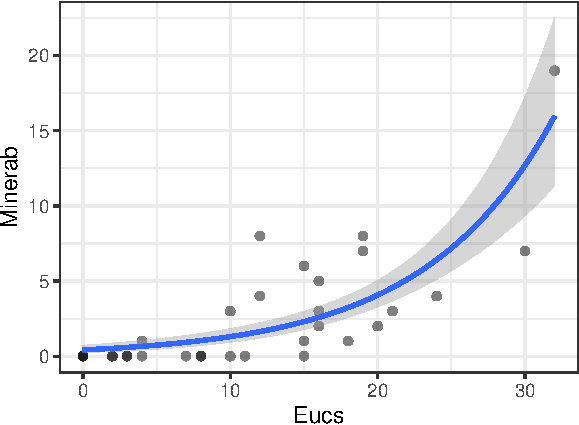
\includegraphics{r-demo-part-4_files/figure-pdf/unnamed-chunk-16-1.pdf}

}

\end{figure}

We can also test the coefficients in the model. The Wald tests for
individual coefficients were already given by the regression summary
above. We might want to carry out likelihood ratio tests for individual
coefficients instead. For example, let's do this for \texttt{Eucs}:

\begin{Shaded}
\begin{Highlighting}[]
\NormalTok{glm\_fit\_partial }\OtherTok{\textless{}{-}} \FunctionTok{glm}\NormalTok{(Minerab }\SpecialCharTok{\textasciitilde{}}\NormalTok{ . }\SpecialCharTok{{-}}\NormalTok{ Miners }\SpecialCharTok{{-}}\NormalTok{ Eucs, }\AttributeTok{family =} \StringTok{"poisson"}\NormalTok{, }\AttributeTok{data =}\NormalTok{ nminer)}
\FunctionTok{anova}\NormalTok{(glm\_fit\_partial, glm\_fit, }\AttributeTok{test =} \StringTok{"LRT"}\NormalTok{)}
\end{Highlighting}
\end{Shaded}

\begin{verbatim}
Analysis of Deviance Table

Model 1: Minerab ~ (Miners + Eucs + Area + Grazed + Shrubs + Bulokes + 
    Timber) - Miners - Eucs
Model 2: Minerab ~ (Miners + Eucs + Area + Grazed + Shrubs + Bulokes + 
    Timber) - Miners
  Resid. Df Resid. Dev Df Deviance  Pr(>Chi)    
1        25     95.513                          
2        24     54.254  1   41.259 1.333e-10 ***
---
Signif. codes:  0 '***' 0.001 '**' 0.01 '*' 0.05 '.' 0.1 ' ' 1
\end{verbatim}

The \texttt{Eucs} variable is quite significant! We can manually carry
out the LRT as a sanity check:

\begin{Shaded}
\begin{Highlighting}[]
\NormalTok{deviance\_partial }\OtherTok{\textless{}{-}}\NormalTok{ glm\_fit\_partial}\SpecialCharTok{$}\NormalTok{deviance}
\NormalTok{deviance\_full }\OtherTok{\textless{}{-}}\NormalTok{ glm\_fit}\SpecialCharTok{$}\NormalTok{deviance}
\NormalTok{lrt\_stat }\OtherTok{\textless{}{-}}\NormalTok{ deviance\_partial }\SpecialCharTok{{-}}\NormalTok{ deviance\_full}
\NormalTok{p\_value }\OtherTok{\textless{}{-}} \FunctionTok{pchisq}\NormalTok{(lrt\_stat, }\AttributeTok{df =} \DecValTok{1}\NormalTok{, }\AttributeTok{lower.tail =} \ConstantTok{FALSE}\NormalTok{)}
\FunctionTok{tibble}\NormalTok{(lrt\_stat, p\_value)}
\end{Highlighting}
\end{Shaded}

\begin{verbatim}
# A tibble: 1 x 2
  lrt_stat  p_value
     <dbl>    <dbl>
1     41.3 1.33e-10
\end{verbatim}

We can test groups of variables using the likelihood ratio test as well.

\part{Generalized linear models: Special cases}

Chapter 4 developed a general theory for GLMs. In Chapter 5, we
specialize this theory to several important cases, including logistic
regression and Poisson regression.

\hypertarget{sec-logistic-regression}{%
\chapter{Logistic regression}\label{sec-logistic-regression}}

\hypertarget{sec-logistic-model}{%
\section{Model definition and interpretation}\label{sec-logistic-model}}

\hypertarget{model-definition}{%
\subsection{Model definition}\label{model-definition}}

Recall from Chapter 4 that the logistic regression model is \[
m_i y_i \overset{\text{ind}} \sim \text{Bin}(m_i, \pi_i); \quad \text{logit}(\pi_i) = \log\frac{\pi_i}{1-\pi_i} = \boldsymbol{x}^T_{i*}\boldsymbol{\beta}.
\] Here we use the canonical logit link function, although other link
functions are possible. We also set the offsets to 0. The interpretation
of the parameter \(\beta_j\) is that a unit increase in \(x_j\)---other
predictors held constant---is associated with an (additive) increase of
\(\beta_j\) on the log-odds scale or a multiplicative increase of
\(e^{\beta_j}\) on the odds scale. Note that logistic regression data
come in two formats: \emph{ungrouped} and \emph{grouped}. For ungrouped
data, we have \(m_1 = \dots = m_n = 1\), so \(y_i \in \{0,1\}\) are
Bernoulli random variables. For grouped data, we can have several
independent Bernoulli observations per predictor
\(\boldsymbol{x}_{i*}\), which give rise to binomial proportions
\(y_i \in [0,1]\). This happens most often when all the predictors are
discrete. You can always convert grouped data into ungrouped data, but
not necessarily vice versa. We'll discuss below that the grouped and
ungrouped formulations of logistic regression have the same MLE and
standard errors but different deviances.

\hypertarget{generative-model-equivalent}{%
\subsection{Generative model
equivalent}\label{generative-model-equivalent}}

Consider the following generative model for
\((\boldsymbol{x}, y) \in \mathbb{R}^{p-1} \times \{0,1\}\): \[
y \sim \text{Ber}(\pi); \quad \boldsymbol{x}|y \sim \begin{cases} N(\boldsymbol{\mu}_0, \boldsymbol{V}) \quad \text{if } y = 0 \\ N(\boldsymbol{\mu}_1, \boldsymbol{V}) \quad \text{if } y = 1 \end{cases}.
\] Then, we can derive that \(y|\boldsymbol{x}\) follows a logistic
regression model (called a \emph{discriminative} model because it
conditions on \(\boldsymbol{x}\)). Indeed, \[
\begin{aligned}
\text{logit}(p(y = 1|\boldsymbol{x})) &= \log\frac{p(y = 1)p(\boldsymbol{x}|y = 1)}{p(y = 0)p(\boldsymbol{x}|y = 0)} \\
&= \log\frac{\pi \exp\left(-\frac12(\boldsymbol{x} - \boldsymbol{\mu}_1)^T \boldsymbol{V}^{-1}(\boldsymbol{x} - \boldsymbol{\mu}_1)\right)}{(1-\pi) \exp\left(-\frac12(\boldsymbol{x} - \boldsymbol{\mu}_0)^T \boldsymbol{V}^{-1}(\boldsymbol{x} - \boldsymbol{\mu}_0)\right)} \\
&= \beta_0 + \boldsymbol{x}^T \boldsymbol{V}^{-1}(\boldsymbol{\mu}_1 - \boldsymbol{\mu}_0) \\
&\equiv \beta_0 + \boldsymbol{x}^T \boldsymbol{\beta}_{-0}.
\end{aligned}
\] This is another natural route to motivating the logistic regression
model.

\hypertarget{sec-2x2-contingency}{%
\subsection{\texorpdfstring{Special case: \(2 \times 2\) contingency
table}{Special case: 2 \textbackslash times 2 contingency table}}\label{sec-2x2-contingency}}

Suppose that \(x \in \{0,1\}\), and consider the logistic regression
model \(\text{logit}(\pi_i) = \beta_0 + \beta_1 x_i\). For example,
suppose that \(x \in \{0,1\}\) encodes treatment (1) and control (0) in
a clinical trial, and \(y_i \in \{0,1\}\) encodes success (1) and
failure (0). We make \(n\) observations of \((x_i, y_i)\) in this
ungrouped setup. The parameter \(e^{\beta_1}\) can be interpreted as the
\emph{odds ratio}: \[
e^{\beta_1} = \frac{\mathbb{P}[y = 1|x=1]/\mathbb{P}[y = 0|x=1]}{\mathbb{P}[y = 1|x=0]/\mathbb{P}[y = 0|x=0]}.
\] This parameter is the multiple by which the odds of success increase
when going from control to treatment. We can summarize such data via the
\(2 \times 2\) \emph{contingency table} (Table~\ref{tbl-2-by-2-table}).
A grouped version of this data would be
\(\{(x_1, y_1) = (0, 7/24), (x_2, y_2) = (1, 9/21)\}\). The null
hypothesis \(H_0: \beta_1 = 0 \Longleftrightarrow H_0: e^{\beta_1} = 1\)
states that the success probability in both rows of the table is the
same.

\hypertarget{tbl-2-by-2-table}{}
\begin{longtable}[]{@{}llll@{}}
\caption{\label{tbl-2-by-2-table}An example of a \(2 \times 2\)
contingency table.}\tabularnewline
\toprule\noalign{}
& Success & Failure & Total \\
\midrule\noalign{}
\endfirsthead
\toprule\noalign{}
& Success & Failure & Total \\
\midrule\noalign{}
\endhead
\bottomrule\noalign{}
\endlastfoot
Treatment & 9 & 12 & 21 \\
Control & 7 & 17 & 24 \\
Total & 16 & 29 & 45 \\
\end{longtable}

\hypertarget{sec-logistic-case-control}{%
\section{Logistic regression with case-control
studies}\label{sec-logistic-case-control}}

In a prospective study (e.g.~a clinical trial), we assign treatment or
control (i.e., \(x\)) to individuals, and then observe a binary outcome
(i.e., \(y\)). Sometimes, the outcome \(y\) takes a long time to measure
or has a highly imbalanced distribution in the population (e.g., the
development of lung cancer). In this case, an appealing study design is
the \emph{retrospective study}, where individuals are sampled based on
their \emph{response values} (e.g., presence of lung cancer) rather than
their treatment/exposure status (e.g., smoking). It turns out that a
logistic regression model is appropriate for such retrospective study
designs as well.

Indeed, suppose that \(y|\boldsymbol{x}\) follows a logistic regression
model. Let's try to figure out the distribution of \(y|\boldsymbol{x}\)
in the retrospectively gathered sample. Letting \(z \in \{0,1\}\) denote
the indicator that an observation is sampled, define
\(\rho_1 \equiv \mathbb{P}[z = 1|y = 1]\) and
\(\rho_0 \equiv \mathbb{P}[z = 1|y = 0]\), and assume that
\(\mathbb{P}[z = 1, y, \boldsymbol{x}] = \mathbb{P}[z = 1 | y]\). The
latter assumption states that the predictors \(\boldsymbol{x}\) were not
used in the retrospective sampling process. Then,

\[
\begin{split}
\text{logit}(\mathbb{P}[y = 1|z = 1, \boldsymbol{x}]) &= \log \frac{\rho_1 \mathbb{P}[y = 1|\boldsymbol{x}]}{\rho_0 \mathbb{P}[y = 0|\boldsymbol{x}]} \\
&= \log \frac{\rho_1}{\rho_0} + \text{logit}(\mathbb{P}[y = 1|\boldsymbol{x}]) \\
&= \left(\log \frac{\rho_1}{\rho_0} + \beta_0\right) + \boldsymbol{x}^T \boldsymbol{\beta}_{-0}.
\end{split}
\]

Thus, conditioning on retrospective sampling changes only the intercept
term, but preserves the coefficients of \(\boldsymbol{x}\). Therefore,
we can carry out inference for \(\boldsymbol{\beta}_{-0}\) in the same
way regardless of whether the study design is prospective or
retrospective.

\hypertarget{sec-estimation-inference}{%
\section{Estimation and inference}\label{sec-estimation-inference}}

\hypertarget{sec-score-fisher}{%
\subsection{Score and Fisher information}\label{sec-score-fisher}}

Recall from Chapter 4 that

\[
\boldsymbol{U}(\boldsymbol{\beta}) = \frac{1}{\phi_0}\boldsymbol{X}^T \boldsymbol{M} \boldsymbol{W} (\boldsymbol{y} - \boldsymbol{\mu}) \quad \text{and} \quad \boldsymbol{I}(\boldsymbol{\beta}) = \frac{1}{\phi_0}\boldsymbol{X}^T \boldsymbol{W} \boldsymbol{X},
\]

where

\[
\begin{aligned}
\boldsymbol{W} &\equiv \text{diag}\left(\frac{w_i}{V(\mu_i)(d\eta_i/d\mu_i)^2}\right), \\
\boldsymbol{M} &\equiv \text{diag}\left(\frac{\partial\eta_i}{\partial \mu_i}\right).
\end{aligned}
\]

Since logistic regression uses a canonical link function, we get the
following simplifications:

\[
\begin{aligned}
\boldsymbol{W} &= \text{diag}\left(w_i V(\mu_i)\right) = \text{diag}\left(m_i \pi_i(1-\pi_i)\right), \\
\boldsymbol{M} &= \text{diag}\left(\frac{1}{\pi_i(1-\pi_i)}\right).
\end{aligned}
\]

Here we have substituted the notation \(\boldsymbol{\pi}\) for
\(\boldsymbol{\mu}\), and recall that for logistic regression,
\(\phi_0 = 1\), \(w_i = m_i\), and \(V(\pi_i) = \pi_i(1-\pi_i)\).
Therefore, the score equations for logistic regression are

\begin{equation}\protect\hypertarget{eq-logistic-score-equations}{}{
0 = \boldsymbol{X}^T \text{diag}\left(m_i\right)(\boldsymbol{y} - \boldsymbol{\widehat{\mu}}) \quad \Longleftrightarrow \quad \sum_{i = 1}^n m_i x_{ij}(y_i-\widehat{\pi}_i) = 0,
}\label{eq-logistic-score-equations}\end{equation} for
\(j = 0, \dots, p-1\). We can solve these equations using IRLS. The
Fisher information is

\[
\boldsymbol{I}(\boldsymbol{\beta}) = \boldsymbol{X}^T \text{diag}\left(m_i \pi_i(1-\pi_i)\right) \boldsymbol{X}.
\]

\hypertarget{sec-wald-inference}{%
\subsection{Wald inference}\label{sec-wald-inference}}

Using the results in the previous paragraph, we can carry out Wald
inference based on the normal approximation

\[
\boldsymbol{\widehat \beta} \overset \cdot \sim N\left(\boldsymbol \beta, \left(\boldsymbol X^T\text{diag}(m_i \widehat \pi_i(1-\widehat \pi_i))\boldsymbol X\right)^{-1}\right).
\]

This approximation holds for \(\sum_{i = 1}^n m_i \rightarrow \infty\).

\hypertarget{sec-2x2-contingency-table}{%
\subsubsection{\texorpdfstring{Example: \(2 \times 2\) contingency
table}{Example: 2 \textbackslash times 2 contingency table}}\label{sec-2x2-contingency-table}}

Suppose we have a \(2 \times 2\) contingency table. The grouped logistic
regression formulation of these data is

\[
y_0 \sim \frac{1}{m_0}\text{Bin}(m_0, \pi_0); \quad y_1 \sim \frac{1}{m_1}\text{Bin}(m_1, \pi_1); \quad \text{logit}(\pi_i) = \beta_0 + \beta_1 x_i.
\]

In this case, we have \(n = p = 2\), so the grouped logistic regression
model is saturated. Therefore, we have

\[
\hat \pi_0 = y_0, \quad \text{and} \quad \hat \pi_1 = y_1, \quad \text{so} \quad \hat \beta_1 = \log \frac{\hat \pi_1 / (1 - \hat \pi_1)}{\hat \pi_0 / (1 - \hat \pi_0)} = \log \frac{y_1 / (1 - y_1)}{y_0 / (1 - y_0)}.
\]

The squared Wald standard error for \(\hat \beta_1\) is

\[
\begin{split}
\text{SE}^2(\widehat \beta_1) &\equiv \left[\left(\boldsymbol X^T\text{diag}(m_i \widehat \pi_i(1-\widehat \pi_i))\boldsymbol X\right)^{-1}\right]_{22} \\
&= \left[\left(\begin{pmatrix} 1 & 0 \\ 1 & 1 \end{pmatrix}^T\begin{pmatrix} m_0y_0(1-y_0) & 0 \\ 0 & m_1y_1(1-y_1) \end{pmatrix}\begin{pmatrix} 1 & 0 \\ 1 & 1 \end{pmatrix}\right)^{-1}\right]_{22} \\
&= \left[\left(\begin{pmatrix} m_0 y_0 (1-y_0) + m_1 y_1 (1-y_1) & m_1 y_1(1-y_1) \\ m_1 y_1(1-y_1) & m_1 y_1(1-y_1) \end{pmatrix}\right)^{-1}\right]_{22} \\
&= \frac{m_0 y_0 (1-y_0) + m_1 y_1 (1-y_1)}{m_0y_0(1-y_0) \cdot m_1y_1(1-y_1)} \\
&= \frac{1}{m_0y_0(1-y_0)} + \frac{1}{m_1y_1(1-y_1)}.
\end{split}
\]

Therefore, the Wald test for \(H_0: \beta_1 = 0\) rejects if

\[
\left|\frac{\hat \beta_1}{\text{SE}(\hat \beta_1)}\right| = \left|\frac{\log \frac{y_1 / (1 - y_1)}{y_0 / (1 - y_0)}}{\sqrt{\frac{1}{m_0y_0(1-y_0)} + \frac{1}{m_1y_1(1-y_1)}}}\right| > z_{1-\alpha/2}.
\]

\hypertarget{sec-hauck-donner-effect}{%
\subsubsection{Hauck-Donner effect}\label{sec-hauck-donner-effect}}

Unfortunately, Wald inference in finite samples does not always perform
very well. The Wald test above is known to be conservative if one or
more of the mean parameters (in this case, \(\pi_i\)) tends to the edge
of the parameter space (in this case, \(\pi_i \rightarrow 0\) or
\(\pi_i \rightarrow 1\)). This is called the \emph{Hauck-Donner effect}.
As an example, consider testing \(H_0: \beta_0 = 0\) in the
intercept-only model

\[
my \sim \text{Bin}(m, \pi); \quad \text{logit}(\pi) = \beta_0.
\]

The Wald test statistic is
\(z \equiv \widehat \beta/\text{SE} = \text{logit}(y)\sqrt{my(1-y)}\).
This test statistic actually tends to \emph{decrease} as
\(y \rightarrow 1\) (see Figure~\ref{fig-hauck-donner}), since the
standard error grows faster than the estimate itself. So the test
statistic becomes less significant as we go further away from the null!
A similar situation arises in the \(2 \times 2\) contingency table
example above, where the Wald test for \(H_0: \beta_1 = 0\) becomes less
significant as \(y_0 \rightarrow 0\) and \(y_1 \rightarrow 1\). As a
limiting case of this, the Wald test is undefined if \(y_0 = 0\) and
\(y_1 = 1\). This situation is a special case of \emph{perfect
separability} in logistic regression: when a hyperplane in covariate
space separates observations with \(y_i = 0\) from those with
\(y_i = 1\). Some of the maximum likelihood coefficient estimates are
infinite in this case, causing the Wald test to be undefined since it
uses these coefficient estimates as test statistics.

\begin{figure}

{\centering \includegraphics{logistic-regression_files/figure-pdf/fig-hauck-donner-1.pdf}

}

\caption{\label{fig-hauck-donner}The Hauck-Donner effect: The Wald
statistic for testing \(H_0: \pi = 0.5\) within the model
\(my \sim \text{Bin}(m, \pi)\) decreases as the proportion \(y\)
approaches 1. Here, \(m = 25\).}

\end{figure}

\hypertarget{sec-likelihood-ratio-inference}{%
\subsection{Likelihood ratio
inference}\label{sec-likelihood-ratio-inference}}

\hypertarget{sec-bernoulli-binomial-deviance}{%
\subsubsection{The Bernoulli and binomial
deviance}\label{sec-bernoulli-binomial-deviance}}

Let's first compute the deviance of a Bernoulli or binomial model. These
deviances are the same because these two models have the same natural
parameter and log-partition function. Recalling the definition of the
unit deviance (\ref{eq-unit-deviance}), we have

\[
\begin{split}
d(y, \mu) &\equiv 2\{[\theta(y) y - \psi(\theta(y))] - [\theta(\mu) y - \psi(\theta(\mu))]\} \\
&= 2\{[y \log\tfrac{y}{1-y} + \log(1-y)] - [y \log \tfrac{\pi}{1-\pi} + \log(1-\pi)]\} \\
&= 2\left(y \log \frac{y}{\pi} + (1-y)\log \frac{1-y}{1-\pi}\right).
\end{split}
\]

The total deviance, therefore, is

\begin{equation}\protect\hypertarget{eq-logistic-deviance}{}{
\begin{split}
D(\boldsymbol y, \hat{\boldsymbol \pi}) &\equiv \sum_{i = 1}^n w_i d(y_i, \widehat \pi_i) \\
&= 2\sum_{i = 1}^n \left(m_i y_i \log \frac{y_i}{\widehat \pi_i} + m_i(1-y_i) \log\frac{1-y_i}{1-\widehat \pi_i}\right).
\end{split}
}\label{eq-logistic-deviance}\end{equation}

\hypertarget{sec-comparing-deviances}{%
\subsubsection{Comparing the deviances of grouped and ungrouped logistic
regression models}\label{sec-comparing-deviances}}

Let us pause to compare the total deviances of grouped and ungrouped
logistic regression models. Consider the following grouped and ungrouped
models:

\[
y^{\text{grp}}_i \overset{\text{ind}} \sim \frac{1}{m_i}\text{Bin}(m_i, \pi_i) \quad \text{and} \quad y^{\text{ungrp}}_{ik} \overset{\text{ind}} \sim \text{Ber}(\pi_i), \quad k = 1, \dots, m_i,
\] where \[
\text{logit}(\pi_i) = \boldsymbol x_{i*}^T \boldsymbol \beta.
\]

The relationship between the grouped and ungrouped observations is that

\[
y^{\text{grp}}_i = \frac{1}{m_i}\sum_{k = 1}^{m_i} y^{\text{ungrp}}_{ik} \equiv \bar y^{\text{ungrp}}_i.
\]

Since the grouped and ungrouped logistic regression models have the same
likelihoods, it follows that they have the same maximum likelihood
estimates \(\widehat{\boldsymbol \beta}\) and
\(\widehat{\boldsymbol \pi}\). However, the total deviances of the two
models are different. The total deviance of the grouped model can be
derived from equation (\ref{eq-logistic-deviance}):

\begin{equation}\protect\hypertarget{eq-total-deviance-grouped}{}{
\begin{split}
&D(\boldsymbol y^{\text{grp}}, \hat{\boldsymbol \pi}) \\
&\quad= 2\sum_{i = 1}^n \left(m_i y^{\text{grp}}_i \log \frac{y^{\text{grp}}_i}{\widehat \pi_i} + m_i(1-y^{\text{grp}}_i) \log\frac{1-y^{\text{grp}}_i}{1-\widehat \pi_i}\right).
\end{split}
}\label{eq-total-deviance-grouped}\end{equation}

On the other hand, the total deviance of the ungrouped model is

\begin{equation}\protect\hypertarget{eq-total-deviance-ungrouped}{}{
\begin{split}
&D(\boldsymbol y^{\text{ungrp}}, \hat{\boldsymbol \pi}) \\
&= 2\sum_{i = 1}^n \sum_{k = 1}^{m_i} \left(y^{\text{ungrp}}_{ik} \log \frac{y^{\text{ungrp}}_{ik}}{\widehat \pi_i} + (1-y^{\text{ungrp}}_{ik}) \log\frac{1-y^{\text{ungrp}}_{ik}}{1-\widehat \pi_i}\right) \\
&= 2\sum_{i = 1}^n \sum_{k = 1}^{m_i} \left(y^{\text{ungrp}}_{ik} \log \frac{1}{\widehat \pi_i} + (1-y^{\text{ungrp}}_{ik}) \log\frac{1}{1-\widehat \pi_i}\right) \\
&= 2\sum_{i = 1}^n \left(m_i y^{\text{grp}}_i \log \frac{1}{\widehat \pi_i} + m_i(1-y^{\text{grp}}_i) \log\frac{1}{1-\widehat \pi_i}\right).
\end{split}
}\label{eq-total-deviance-ungrouped}\end{equation}

In the second line, we used the fact that \(y \log y \rightarrow 0\) and
\((1-y)\log(1-y) \rightarrow 0\) as \(y \rightarrow 0\) or
\(y \rightarrow 1\). Comparing the grouped
(\ref{eq-total-deviance-grouped}) and ungrouped
(\ref{eq-total-deviance-ungrouped}) total deviances, we see that these
are given by related, but different expressions. Because small
dispersion asymptotics applies to the grouped model but not the
ungrouped model, we have that under small-dispersion asymptotics,

\[
D(\boldsymbol y^{\text{grp}}, \hat{\boldsymbol \pi}) \overset \cdot \sim \chi^2_{n-p} \quad \text{but} \quad D(\boldsymbol y^{\text{ungrp}}, \hat{\boldsymbol \pi}) \not \sim \chi^2_{n-p}.
\]

\hypertarget{sec-likelihood-ratio-test}{%
\subsubsection{Likelihood ratio inference for one or more
coefficients}\label{sec-likelihood-ratio-test}}

Letting \(\boldsymbol{\widehat \pi}_0\) and
\(\boldsymbol{\widehat \pi}_1\) be the MLEs from two nested models, we
can then express the likelihood ratio statistic as

\[
D(\boldsymbol y, \boldsymbol{\widehat \pi}_0) - D(\boldsymbol y, \boldsymbol{\widehat \pi}_1) = 2\sum_{i = 1}^n \left(m_i y_i \log \frac{\widehat \pi_{i1}}{\widehat \pi_{i0}} + m_i(1-y_i) \log\frac{1-\widehat \pi_{i1}}{1-\widehat \pi_{i0}}\right).
\]

Note that this expression holds for grouped or ungrouped logistic
regression models. We can then construct a likelihood ratio test in the
usual way. Likelihood ratio inference can be justified by either
large-sample or small-dispersion asymptotics.

\hypertarget{sec-goodness-of-fit}{%
\subsubsection{Goodness of fit testing}\label{sec-goodness-of-fit}}

In grouped logistic regression, we can also use the likelihood ratio
test to test goodness of fit. To do so, we compare the total deviance of
the fitted model (\ref{eq-logistic-deviance}) to a chi-squared quantile.
In particular, the deviance-based goodness of fit test rejects when:

\begin{equation}\protect\hypertarget{eq-goodness-of-fit}{}{
\begin{split}
&D(\boldsymbol{y}, \hat{\boldsymbol{\pi}}) = \\
&2\sum_{i = 1}^n \left(m_i y_i \log \frac{y_i}{\widehat \pi_i} + m_i(1-y_i) \log\frac{1-y_i}{1-\widehat \pi_i}\right) > \chi^2_{n-p}(1-\alpha).
\end{split}
}\label{eq-goodness-of-fit}\end{equation}

This test is justified by small-dispersion asymptotics based on the
saddlepoint approximation, which is decent when
\(\min(m_i \widehat \pi_i, (1-m_i)\widehat \pi_i) \geq 3\) for each
\(i\).

\hypertarget{sec-example-2x2-table}{%
\subsubsection{\texorpdfstring{Example: \(2 \times 2\)
table}{Example: 2 \textbackslash times 2 table}}\label{sec-example-2x2-table}}

Let us revisit the example of the \(2 \times 2\) table model, within
which we would like to test \(H_0: \beta_1 = 0\). Note that we can view
this as a goodness of fit test of the intercept-only model in a grouped
logistic regression model since the alternative model is the saturated
model (it has two observations and two parameters). To compute the
likelihood ratio statistic, we first need to fit the intercept-only
model. The score equations (\ref{eq-logistic-score-equations}) reduce
to:

\[
m_0 (y_0 - \hat \pi) + m_1 (y_1 - \hat \pi) = 0 \quad \Longrightarrow \quad \hat \pi_0 = \hat \pi_1 = \hat \pi = \frac{m_0 y_0 + m_1 y_1}{m_0 + m_1}.
\]

Therefore, the deviance-based test of \(H_0: \beta_1 = 0\) rejects when:

\[
\begin{split}
D(\boldsymbol{y}, \boldsymbol{\widehat \pi}) &= 2\sum_{i = 1}^n \left(m_i y_i \log \frac{y_i}{\widehat \pi_i} + m_i(1-y_i) \log\frac{1-y_i}{1-\widehat \pi_i}\right) \\
&= 2\left(m_0 y_0 \log\frac{y_0}{\hat \pi} + m_0(1-y_0)\log\frac{1-y_0}{1-\hat \pi}\right) + \\
&\quad \quad 2\left(m_1 y_1 \log\frac{y_1}{\hat \pi} + m_1(1-y_1)\log\frac{1-y_1}{1-\hat \pi}\right) \\
&> \chi^2_{1}(1-\alpha).
\end{split}
\]

Likelihood ratio inference can give nontrivial conclusions in cases when
Wald inference cannot, e.g.~in the case of perfect separability. In the
above example, suppose \(y_0 = 0\) and \(y_1 = 1\), giving perfect
separability. Then, we can use the fact that \(y \log y \rightarrow 0\)
and \((1-y)\log(1-y) \rightarrow 0\) as \(y \rightarrow 0\) or
\(y \rightarrow 1\) to see that:

\begin{equation}\protect\hypertarget{eq-perfect-separability}{}{
\begin{split}
D(\boldsymbol{y}, \boldsymbol{\widehat \pi}) &= 2\left(m_0 \log\frac{1}{1-\hat \pi} + m_1 \log\frac{1}{\hat \pi}\right) \\
&= 2\left(m_0 \log \frac{m_0 + m_1}{m_0} + m_1 \log \frac{m_0 + m_1}{m_1}\right).
\end{split}
}\label{eq-perfect-separability}\end{equation}

This gives us a finite value, which we can compare to
\(\chi^2_{1}(1-\alpha)\) to test \(H_0: \beta_1 = 0\). Even though the
likelihood ratio statistic is still defined, we do still have to be
careful because the data may suggest that the parameters are too close
to the boundary of the parameter space. However, the rate at which the
test breaks down as the parameters approach this boundary is slower than
the rate at which the Wald test breaks down.

\hypertarget{sec-score-based-inference}{%
\subsection{Score-based inference}\label{sec-score-based-inference}}

Here we present only the score-based goodness-of-fit test. Recalling
Section~\ref{sec-score-goodness-of-fit}, the score statistic for
goodness of fit is Pearson's \(X^2\) statistic:

\begin{equation}\protect\hypertarget{eq-pearson-statistic}{}{
X^2 = \sum_{i = 1}^n \frac{w_i (y_i - \widehat \mu_i)^2}{V(\widehat \mu_i)} = \sum_{i = 1}^n \frac{m_i(y_i - \widehat \pi_i)^2}{\widehat \pi_i(1-\widehat \pi_i)}.
}\label{eq-pearson-statistic}\end{equation}

This test is justified by small-dispersion asymptotics based on the
central limit theorem, which is decent when
\(\min(m_i \pi_i, (1-m_i)\pi_i) \geq 5\) for each \(i\).

\hypertarget{sec-fisher-exact-test}{%
\subsection{Fisher's exact test}\label{sec-fisher-exact-test}}

As an alternative to asymptotic tests for logistic regression, in the
case of \(2 \times 2\) tables, there is an \emph{exact} test of
\(H_0: \beta_1 = 0\). Suppose we have:

\begin{equation}\protect\hypertarget{eq-binomial}{}{
s_1 = m_1y_1 \sim \text{Bin}(m_1, \pi_1) \quad \text{and} \quad s_2 = m_2y_2 \sim \text{Bin}(m_2, \pi_2).
}\label{eq-binomial}\end{equation}

The trick is to conduct inference \emph{conditional on} \(s_1 + s_2\).
Note that under \(H_0: \pi_1 = \pi_2\), we have:

\begin{equation}\protect\hypertarget{eq-exact-test}{}{
\begin{split}
&\mathbb{P}[s_1 = t | s_1+s_2 = v] \\
&\quad= \mathbb{P}[s_1 = t | s_1 + s_2 = v] \\
&\quad= \frac{\mathbb{P}[s_1 = t, s_2 = v-t]}{\mathbb{P}[s_1 + s_2 = v]} \\
&\quad= \frac{{m_1 \choose t}\pi^{t}(1-\pi)^{m_1 - t}{m_2 \choose v-t}\pi^{v-t}(1-\pi)^{m_2 - (v-t)}}{{m_1 + m_2 \choose v}\pi^v (1-\pi)^{m_1 + m_2 - v}} \\
&\quad= \frac{{m_1 \choose t}{m_2 \choose v-t}}{{m_1 + m_2 \choose v}}.
\end{split}
}\label{eq-exact-test}\end{equation}

Therefore, a finite-sample \(p\)-value to test \(H_0: \pi_1 = \pi_2\)
versus \(H_1: \pi_1 > \pi_2\) is \(\mathbb{P}[s_1 \geq t | s_1 + s_2]\),
which can be computed exactly based on the formula above.

\hypertarget{sec-poisson-regression}{%
\chapter{Poisson regression}\label{sec-poisson-regression}}

\hypertarget{sec-model-definition}{%
\section{Model definition and
interpretation}\label{sec-model-definition}}

The Poisson regression model (with offsets) is:

\begin{equation}\protect\hypertarget{eq-poisson-with-offsets}{}{
y_i \overset{\text{ind}}\sim \text{Poi}(\mu_i); \quad \log \mu_i = o_i + \boldsymbol{x}_{i*}^T \boldsymbol{\beta}.
}\label{eq-poisson-with-offsets}\end{equation}

Because the log of the mean is linear in the predictors, Poisson
regression models are often called \emph{loglinear models}. To interpret
the coefficients, note that a unit increase in \(x_j\) (while keeping
the other variables fixed) is associated with an increase in the
predicted mean by a factor of \(e^{\beta_j}\).

\hypertarget{sec-example-modeling-rates}{%
\section{Example: Modeling rates}\label{sec-example-modeling-rates}}

One cool feature of the Poisson model is that rates can be easily
modeled with the help of offsets. Let's say that the count \(y_i\) is
collected over the course of a time interval of length \(t_i\), or a
spatial region with area \(t_i\), or a population of size \(t_i\), etc.
Then, it is meaningful to model:

\[
y_i \overset{\text{ind}} \sim \text{Poi}(\pi_i t_i), \quad \log \pi_i = \boldsymbol{x}^T_{i*}\boldsymbol{\beta},
\]

where \(\pi_i\) represents the rate of events per day / per square mile
/ per capita, etc. In other words:

\[
y_i \overset{\text{ind}} \sim \text{Poi}(\mu_i), \quad \log \mu_i = \log t_i + \boldsymbol{x}^T_{i*}\boldsymbol{\beta},
\]

which is exactly equation (\ref{eq-poisson-with-offsets}) with offsets
\(o_i = \log t_i\). For example, in single-cell RNA-sequencing, \(y_i\)
is the number of RNA molecules aligning to a gene in cell \(i\) and
\(t_i\) is the total number of RNA molecules measured in the cell, a
quantity called the \emph{library size}. We might use a Poisson
regression model to carry out a \emph{differential expression analysis}
between two cell types.

\hypertarget{sec-estimation-inference}{%
\section{Estimation and inference}\label{sec-estimation-inference}}

\hypertarget{sec-wald-inference}{%
\subsection{Score, Fisher information, and Wald
inference}\label{sec-wald-inference}}

We found in Chapter 4 that the score and Fisher information for Poisson
regression are:

\[
\boldsymbol{U}(\boldsymbol{ \beta}) = \boldsymbol{X}^T(\boldsymbol{y} - \boldsymbol{\mu}),
\]

and:

\[
\boldsymbol{I}(\boldsymbol{\beta}) = \boldsymbol{X}^T \boldsymbol{W} \boldsymbol{X} = \boldsymbol{X}^T \text{diag}(V(\mu_i))\boldsymbol{X} = \boldsymbol{X}^T \text{diag}(\mu_i)\boldsymbol{X},
\]

respectively. Hence, the normal equations for the MLE are:

\[
\boldsymbol{X}^T(\boldsymbol{y} - \boldsymbol{\hat \mu}).
\]

Wald inference is based on the approximation:

\[
\boldsymbol{\hat \beta} \overset \cdot \sim N(\boldsymbol{\beta}, (\boldsymbol{X}^T \text{diag}(\hat \mu_i)\boldsymbol{X})^{-1}).
\]

\hypertarget{sec-likelihood-ratio-inference}{%
\subsection{Likelihood ratio
inference}\label{sec-likelihood-ratio-inference}}

For likelihood ratio inference, we first derive the total deviance. The
unit deviance of a Poisson distribution is:

\[
d(y, \mu) = 2\left(y \log \frac{y}{\mu} - (y - \mu)\right).
\]

Hence, the total deviance is:

\[
D(\boldsymbol{y}, \boldsymbol{\mu}) = \sum_{i = 1}^n d(y_i, \mu_i) = 2\sum_{i = 1}^n \left(y_i \log \frac{y_i}{\mu_i} - (y_i - \mu_i)\right).
\]

The residual deviance is then:

\[
D(\boldsymbol{y}, \boldsymbol{\hat\mu}) = 2\sum_{i = 1}^n \left(y_i \log \frac{y_i}{\hat \mu_i} - (y_i - \hat \mu_i)\right) = 2\sum_{i = 1}^n y_i \log \frac{y_i}{\hat \mu_i}.
\]

The last equality holds for any model containing the intercept, since by
the normal equations we have
\(\sum_{i = 1}^n (y_i - \hat \mu_i) = \boldsymbol{1}^T (\boldsymbol{y} - \boldsymbol{\hat \mu}) = 0\).
We can carry out a likelihood ratio test for
\(H_0: \boldsymbol \beta_S = \boldsymbol{0}\) via:

\[
D(\boldsymbol{y}, \boldsymbol{\hat \mu}^0) - D(\boldsymbol{y}, \boldsymbol{\hat \mu}) = 2\sum_{i = 1}^n y_i \log \frac{\hat \mu_i}{\hat \mu^0_{i}} \overset{\cdot}\sim \chi^2_{|S|}.
\]

We can carry out a goodness-of-fit test via:

\[
D(\boldsymbol{y}, \boldsymbol{\hat\mu}) = 2\sum_{i = 1}^n y_i \log \frac{y_i}{\hat \mu_i} \overset{\cdot}\sim \chi^2_{n - p}.
\] This approximation is justified by the saddlepoint approximation in
small-dispersion asymptotics, which is reliable if \(\hat \mu_i \geq 3\)
for all \(i\).

\hypertarget{sec-score-based-inference}{%
\subsection{Score-based inference}\label{sec-score-based-inference}}

Recalling Section~\ref{sec-score-test-single-coeff}, the score test for
\(H_0: \beta_j = 0\) is based on the approximation \[
\frac{\boldsymbol{x}_{*,j}^T (\boldsymbol{y} - \boldsymbol{\widehat{\mu}}^0)}{\sqrt{\boldsymbol x_{*,j}^T \boldsymbol {\widehat W}^{0}\boldsymbol x_{*,j} - \boldsymbol x_{*,j}^T \boldsymbol {\widehat W}^{0}\boldsymbol X_{*,\text{-}j}(\boldsymbol X_{*,\text{-}j}^T \boldsymbol {\widehat W}^{0}\boldsymbol X_{*,\text{-}j})^{-1}\boldsymbol X_{*,\text{-}j}^T \boldsymbol {\widehat W}^{0}\boldsymbol x_{*,j}}} \overset{\cdot}\sim N(0,1),
\] where \[
\boldsymbol {\widehat W}^{0} = \text{diag}(\boldsymbol{\widehat{\mu}}^0).
\]

On the other hand, the score test for goodness-of-fit is based on the
Pearson \(X^2\) statistic:

\[
X^2 \equiv \sum_{i = 1}^n \frac{(y_i - \hat \mu_i)^2}{\hat \mu_i} \overset{\cdot}\sim \chi^2_{n - p}.
\] This approximation is justified by the central limit theorem in
small-dispersion asymptotics, which is reliable if \(\hat \mu_i \geq 5\)
for all \(i\).

\hypertarget{sec-poisson-multinomial}{%
\section{Relationship between Poisson and multinomial
distributions}\label{sec-poisson-multinomial}}

Suppose that \(y_i \overset{\text{ind}}\sim \text{Poi}(\mu_i)\) for
\(i = 1, \dots, n\). Then,

\[
\begin{split}
\mathbb{P}\left[y_1 = m_1, \dots, y_n = m_n \left| \sum_{i}y_i = m\right.\right] &= \frac{\mathbb{P}[y_1 = m_1, \dots, y_n = m_n]}{\mathbb{P}[\sum_{i}y_i = m]} \\
&= \frac{\prod_{i = 1}^n e^{-\mu_i}\frac{\mu_i^{m_i}}{m_i!}}{e^{-\sum_i \mu_i}\frac{(\sum_i \mu_i)^m}{m!}} \\
&= {m \choose m_1, \dots, m_n} \prod_{i = 1}^n \pi_i^{m_i},
\end{split}
\] where \[
\pi_i \equiv \frac{\mu_i}{\sum_{i' = 1}^n \mu_{i'}}.
\] We recognize the last expression in the previous display as the
probability mass function of the multinomial distribution with
parameters \((\pi_1, \dots, \pi_n)\) summing to one. In words, the joint
distribution of a set of independent Poisson distributions conditional
on their sum is a multinomial distribution.

\hypertarget{sec-example-2x2-tables}{%
\section{\texorpdfstring{Example: \(2 \times 2\) contingency
tables}{Example: 2 \textbackslash times 2 contingency tables}}\label{sec-example-2x2-tables}}

\hypertarget{sec-poisson-2x2}{%
\subsection{\texorpdfstring{Poisson model for \(2 \times 2\) contingency
tables}{Poisson model for 2 \textbackslash times 2 contingency tables}}\label{sec-poisson-2x2}}

Let's say that we have two binary random variables
\(x_1, x_2 \in \{0,1\}\) with joint distribution
\(\mathbb{P}(x_1 = j, x_2 = k) = \pi_{jk}\) for \(j,k \in \{0,1\}\). We
collect a total of \(m\) samples from this joint distribution and
summarize the counts in a \(2 \times 2\) table, where \(y_{jk}\) is the
number of times we observed \((x_1, x_2) = (j,k)\), so that:

\[
(y_{00}, y_{01}, y_{10}, y_{11}) \sim \text{Mult}(m, (\pi_{00}, \pi_{01}, \pi_{10}, \pi_{11})).
\]

Our primary question is whether these two random variables are
independent, i.e.

\begin{equation}\protect\hypertarget{eq-null-product-formulation}{}{
\pi_{jk} = \pi_{j+}\pi_{+k},
}\label{eq-null-product-formulation}\end{equation} where \[
\pi_{j+} \equiv \mathbb{P}[x_1 = j] = \pi_{j1} + \pi_{j2}; \quad \pi_{+k} \equiv \mathbb{P}[x_2 = k] = \pi_{1k} + \pi_{2k}.
\]

We can express this equivalently as:

\[
\pi_{00}\pi_{11} = \pi_{01}\pi_{10}.
\]

In other words, we can express the independence hypothesis concisely as:

\begin{equation}\protect\hypertarget{eq-independence-2}{}{
H_0: \frac{\pi_{11}\pi_{00}}{\pi_{10}\pi_{01}} = 1.
}\label{eq-independence-2}\end{equation}

Let's arbitrarily assume that, additionally,
\(m \sim \text{Poi}(\mu_{++})\). Then, by the relationship between
Poisson and multinomial distributions, we have:

\[
y_{jk} \overset{\text{ind}} \sim \text{Poi}(\mu_{++}\pi_{jk}).
\]

Let \(i \in \{1,2,3,4\}\) index the four pairs \[
(x_1, x_2) \in \{(0,0), (0,1), (1,0), (1,1)\},
\] so that for \(i = 1, \dots, 4\), we have
\begin{equation}\protect\hypertarget{eq-2x2-poisson-reg}{}{
y_i \overset{\text{ind}}\sim \text{Poi}(\mu_i); \quad \log \mu_i = \beta_0 + \beta_1 x_{i1} + \beta_2 x_{i2} + \beta_{12}x_{i1} x_{i2},
}\label{eq-2x2-poisson-reg}\end{equation}

where:

\begin{equation}\protect\hypertarget{eq-2x2-poisson-reg-coefs}{}{
\begin{aligned}
\beta_0 = \log \mu_{++} + \log \pi_{00}; \quad \beta_1 = \log \frac{\pi_{10}}{\pi_{00}}; \\
\beta_2 = \log \frac{\pi_{01}}{\pi_{00}}; \quad \beta_{12} = \log\frac{\pi_{11}\pi_{00}}{\pi_{10}\pi_{01}}.
\end{aligned}
}\label{eq-2x2-poisson-reg-coefs}\end{equation}

Note that the independence hypothesis (\ref{eq-independence-2}) reduces
to the hypothesis \(H_0: \beta_{12} = 0\):

\[
H_0: \frac{\pi_{11}\pi_{00}}{\pi_{10}\pi_{01}} = 1 \quad \Longleftrightarrow \quad H_0: \beta_{12} = 0.
\]

So the presence of an interaction in the Poisson regression is
equivalent to a lack of independence between \(x_1\) and \(x_2\). We can
test the latter hypothesis using our standard tools for Poisson
regression.

For example, we can use the Pearson \(X^2\) goodness-of-fit test. To
apply this test, we must find the fitted means under the null hypothesis
model:

\begin{equation}\protect\hypertarget{eq-2x2-poisson-reg-null}{}{
y_i \overset{\text{ind}}\sim \text{Poi}(\mu_i); \quad \log \mu_i = \beta_0 + \beta_1 x_{i1} + \beta_2 x_{i2}, \quad i = 1, \dots, 4.
}\label{eq-2x2-poisson-reg-null}\end{equation}

The normal equations give us the following:

\[
\begin{aligned}
y_{++} &\equiv \sum_{j, k = 0}^1 y_{jk} = \sum_{j, k = 0}^1 \hat \mu_{jk} \equiv \hat \mu_{++}; \\
y_{+1} &\equiv \sum_{j = 0}^1 y_{j1} = \sum_{j = 0}^1 \hat \mu_{j1} \equiv \hat \mu_{+1}; \\
y_{1+} &\equiv \sum_{k = 0}^1 y_{1k} = \sum_{k = 0}^1 \hat \mu_{1k} \equiv \hat \mu_{1+}.
\end{aligned}
\]

By combining these equations, we arrive at:

\[
\hat \mu_{++} = y_{++}; \quad \hat \mu_{j+} = y_{j+} \text{ for all } j \in \{0, 1\}; \quad \hat \mu_{+k} = y_{+k} \text{ for all } k \in \{0, 1\}.
\]

Therefore, the fitted means under the null hypothesis model
\ref{eq-2x2-poisson-reg-null} are:

\[
\hat \mu_{jk} = \hat \mu_{++}\hat \pi_{jk} = \hat \mu_{++}\hat \pi_{j+}\hat \pi_{+k} = y_{++}\frac{y_{j+}}{y_{++}}\frac{y_{+k}}{y_{++}} = \frac{y_{j+}y_{+k}}{y_{++}}.
\]

Hence, we have:

\[
X^2 = \sum_{j,k = 0}^1 \frac{(y_{jk} - \widehat \mu_{jk})^2}{\widehat \mu_{jk}} = \sum_{j, k = 0}^1 \frac{(y_{jk} - y_{j+}y_{+k}/y_{++})^2}{y_{j+}y_{+k}/y_{++}}.
\]

Alternatively, we can use the likelihood ratio test, which gives:

\[
G^2 = 2\sum_{j,k = 0}^1 y_{jk}\log\frac{y_{jk}}{\widehat \mu_{jk}} = 2\sum_{j, k = 0}^1 y_{jk}\log\frac{y_{jk}}{y_{j+}y_{+k}/y_{++}}.
\]

We would compare both \(X^2\) and \(G^2\) to a \(\chi^2_1\)
distribution.

\hypertarget{sec-inference-conditioning-margins}{%
\subsection{Inference is the same regardless of conditioning on
margins}\label{sec-inference-conditioning-margins}}

Now, our data might actually have been collected such that
\(n \sim \text{Poi}(\mu_{++})\), or maybe \(n\) was fixed in advance. Is
the Poisson inference proposed above actually valid in the latter case?
In fact, it is! To see this, let us consider the log likelihoods of the
two models:

\[
p_{\boldsymbol{\mu}}(\boldsymbol{y}) = p_{\mu_{++}}(y_{++} = n)p_{\boldsymbol{\pi}}(\boldsymbol{y} | y_{++} = n),
\]

so:

\[
\begin{split}
\log p_{\boldsymbol{\mu}}(\boldsymbol{y}) &= \log p_{\mu_{++}}(y_{++} = n) + \log p_{\boldsymbol{\pi}}(\boldsymbol{y} | y_{++} = n) \\
&= C + \log p_{\boldsymbol{\pi}}(\boldsymbol{y} | y_{++} = n).
\end{split}
\]

In other words, the log-likelihoods of the Poisson and multinomial
models, as a function of \(\boldsymbol{\pi}\), differ from each other by
a constant. Therefore, any likelihood-based inference in these models is
equivalent. The same argument shows that conditioning on the row or
column totals (as opposed to the overall total) also yields the same
exact inference. Therefore, regardless of the sampling mechanism, we can
always conduct an independence test in a \(2 \times 2\) table via a
Poisson regression.

\hypertarget{sec-poisson-logistic-equivalence}{%
\subsection{Equivalence among Poisson and logistic
regressions}\label{sec-poisson-logistic-equivalence}}

We've talked about two ways to view a \(2 \times 2\) contingency table.
In the logistic regression view, we thought about one variable as a
predictor and the other as a response, seeking to test whether the
predictor has an impact on the response. In the Poisson regression view,
we thought about the two variables symmetrically, seeking to test
independence. It turns out that these two perspectives are equivalent.
Recall that we have derived in equations \ref{eq-2x2-poisson-reg} and
\ref{eq-2x2-poisson-reg-coefs} that \(x_1 \perp \!\!\! \perp x_2\) if
and only if \(\beta_{12} = 0\) in the Poisson regression:

\[
\log y_i \overset{\text{ind}}{\sim} \text{Poi}(\mu_i), \quad \log \mu_i = \beta_0 + \beta_1 x_{i1} + \beta_2 x_{i2} + \beta_{12} x_{i1}x_{i2}, \quad i = 1, \dots, 4.
\]

However, we have:

\[
\begin{split}
\beta_{12} &= \log \frac{\pi_{11}\pi_{00}}{\pi_{01}\pi_{10}} \\
&= \log \frac{\pi_{11}/\pi_{01}}{\pi_{01}/\pi_{00}} = \log \frac{\mathbb{P}[x_2 = 1 \mid x_1 = 1] / \mathbb{P}[x_2 = 0 \mid x_1 = 1]}{\mathbb{P}[x_2 = 1 \mid x_1 = 0] / \mathbb{P}[x_2 = 0 \mid x_1 = 0]}.
\end{split}
\]

Recalling the logistic regression of \(x_2\) on \(x_1\):

\begin{equation}\protect\hypertarget{eq-2x2-logistic-reg}{}{
\text{logit } \mathbb{P}[x_2 = 1 \mid x_1] = \tilde{\beta_0} + \tilde{\beta_1} x_1,
}\label{eq-2x2-logistic-reg}\end{equation}

and that \(\tilde{\beta_1}\) is the log odds ratio, we conclude that:

\[
\beta_{12} = \tilde{\beta_1},
\]

so \(x_1 \perp \!\!\! \perp x_2\) if and only if
\(\tilde{\beta_1} = 0\). Due to the equivalence between Poisson and
multinomial distributions, the hypothesis tests and confidence intervals
for the log odds ratio \(\beta_{12}\) (or \(\tilde{\beta_1}\)) obtained
from Poisson and logistic regressions will be the same.

\hypertarget{sec-poisson-jk-tables}{%
\section{\texorpdfstring{Example: Poisson models for \(J \times K\)
contingency
tables}{Example: Poisson models for J \textbackslash times K contingency tables}}\label{sec-poisson-jk-tables}}

Suppose now that \(x_1 \in \{0, 1, \dots, J-1\}\) and
\(x_2 \in \{0, 1, \dots, K-1\}\). Then, we denote
\(\mathbb{P}[x_1 = j, x_2 = k] = \pi_{jk}\). We still are interested in
testing for independence between \(j\) and \(k\), which amounts to a
goodness-of-fit test for the Poisson model:

\[
y_{jk} \overset{\text{ind}}\sim \text{Poi}(\mu_{jk}); \quad \log \mu_{jk} = \beta_0 + \beta^1_j + \beta^2_k.
\]

The score (Pearson) and deviance-based goodness-of-fit statistics for
this test are:

\[
X^2 = \sum_{j = 0}^{J-1} \sum_{k = 0}^{K-1} \frac{(y_{jk} - \widehat \mu_{jk})^2}{\widehat \mu_{jk}} \quad \text{and} \quad G^2 = 2\sum_{j = 0}^{J-1} \sum_{k = 0}^{K-1} y_{jk}\log \frac{y_{jk}}{\widehat \mu_{jk}},
\]

where
\(\widehat \mu_{jk} = \widehat y_{++}\frac{y_{j+}}{y_{++}}\frac{y_{+k}}{y_{++}}\).
Like with the \(2 \times 2\) case, the test is the same regardless of
whether we condition on the row sums, column sums, total count, or if we
do not condition at all. The degrees of freedom in the full model is
\(JK\), while the degrees of freedom in the partial model is
\(J + K - 1\), so the degrees of freedom for the goodness-of-fit test is
\(JK - J - K + 1 = (J - 1)(K - 1)\). Pearson erroneously concluded that
the test had \(JK - 1\) degrees of freedom, which, when Fisher corrected
it, created a lot of animosity between these two statisticians.

\hypertarget{sec-poisson-jkl-tables}{%
\section{\texorpdfstring{Example: Poisson models for
\(J \times K \times L\) contingency
tables}{Example: Poisson models for J \textbackslash times K \textbackslash times L contingency tables}}\label{sec-poisson-jkl-tables}}

These ideas can be extended to multi-way tables, for example, three-way
tables. If we have \(x_1 \in \{0, 1, \dots, J-1\}\),
\(x_2 \in \{0, 1, \dots, K-1\}\), \(x_3 \in \{0, 1, \dots, L-1\}\), then
we might be interested in testing several kinds of null hypotheses:

\begin{itemize}
\tightlist
\item
  Mutual independence:
  \(H_0: x_1 \perp \!\!\! \perp x_2 \perp \!\!\! \perp x_3\).
\item
  Joint independence: \(H_0: x_1 \perp \!\!\! \perp (x_2, x_3)\).
\item
  Conditional independence:
  \(H_0: x_1 \perp \!\!\! \perp x_2 \mid x_3\).
\end{itemize}

These three null hypotheses can be shown to be equivalent to the Poisson
regression model:

\[
y_{jkl} \overset{\text{ind}}\sim \text{Poi}(\mu_{jkl}),
\]

where:

\[
\log \mu_{jkl} = \beta_0 + \beta^1_j + \beta^2_k + \beta^3_l \quad \text{(mutual independence)};
\]

\[
\log \mu_{jkl} = \beta_0 + \beta^1_j + \beta^2_k + \beta^3_l + \beta^{2,3}_{kl} \quad \text{(joint independence)};
\]

\[
\log \mu_{jkl} = \beta_0 + \beta^1_j + \beta^2_k + \beta^3_l + \beta^{1,3}_{jl} + \beta^{2,3}_l \quad \text{(conditional independence)}.
\]

\hypertarget{sec-nb-regression}{%
\chapter{Negative binomial regression}\label{sec-nb-regression}}

\hypertarget{overdispersion}{%
\section{Overdispersion}\label{overdispersion}}

A pervasive issue with Poisson regression is \emph{overdispersion}: that
the variances of observations are greater than the corresponding means.
A common cause of overdispersion is omitted variable bias. Suppose that
\(y \sim \text{Poi}(\mu)\), where
\(\log \mu = \beta_0 + \beta_1 x_1 + \beta_2 x_2\). However, we omitted
variable \(x_2\) and are considering the GLM based on
\(\log \mu = \beta_0 + \beta_1 x_1\). If \(\beta_2 \neq 0\) and \(x_2\)
is correlated with \(x_1\), then we have a confounding issue. Let's
consider the more benign situation that \(x_2\) is independent of
\(x_1\). Then, we have

\begin{equation}\protect\hypertarget{eq-mean-variance}{}{
\begin{split}
\mathbb{E}[y|x_1] &= \mathbb{E}[\mathbb{E}[y|x_1, x_2]|x_1] \\
&= \mathbb{E}[e^{\beta_0 + \beta_1 x_1 + \beta_2 x_2}|x_1] \\
&= e^{\beta_0 + \beta_1 x_1}\mathbb{E}[e^{\beta_2 x_2}] = e^{\beta'_0 + \beta_1 x_1}.
\end{split}
}\label{eq-mean-variance}\end{equation}

So in the model for the mean of \(y\), the impact of omitted variable
\(x_2\) seems only to have impacted the intercept. Let's consider the
variance of \(y\):

\begin{equation}\protect\hypertarget{eq-var-greater-mean}{}{
\begin{split}
\text{Var}[y|x_1] &= \mathbb{E}[\text{Var}[y|x_1, x_2]|x_1] + \text{Var}[\mathbb{E}[y|x_1, x_2]|x_1] \\
&= e^{\beta'_0 + \beta_1 x_1} + e^{2(\beta'_0 + \beta_1 x_1)}\text{Var}[e^{\beta_2 x_2}] \\
&> e^{\beta'_0 + \beta_1 x_1} \\
&= \mathbb{E}[y|x_1].
\end{split}
}\label{eq-var-greater-mean}\end{equation}

So indeed, the variance is larger than what we would have expected under
the Poisson model.

\hypertarget{hierarchical-poisson-regression}{%
\section{Hierarchical Poisson
regression}\label{hierarchical-poisson-regression}}

Let's say that \(y|\boldsymbol{x} \sim \text{Poi}(\lambda)\), where
\(\lambda|\boldsymbol{x}\) is random due to the fluctuations of the
omitted variables. A common distribution used to model nonnegative
random variables is the \emph{gamma} distribution \(\Gamma(\mu, k)\),
parameterized by a mean \(\mu > 0\) and a \emph{shape} \(k > 0\). This
distribution has probability density function

\begin{equation}\protect\hypertarget{eq-gamma-pdf}{}{
f(\lambda; k, \mu) = \frac{(k/\mu)^k}{\Gamma(k)}e^{-k\lambda/\mu}\lambda^{k-1},
}\label{eq-gamma-pdf}\end{equation}

with mean and variance given by

\begin{equation}\protect\hypertarget{eq-gamma-moments}{}{
\mathbb{E}[\lambda] = \mu; \quad \text{Var}[\lambda] = \mu^2/k.
}\label{eq-gamma-moments}\end{equation}

Therefore, it makes sense to augment the Poisson regression model as
follows:

\begin{equation}\protect\hypertarget{eq-nb-hierarchical}{}{
\lambda|\boldsymbol{x} \sim \Gamma(\mu, k), \quad \log \mu = \boldsymbol{x}^T \boldsymbol{\beta}, \quad y | \lambda \sim \text{Poi}(\lambda).
}\label{eq-nb-hierarchical}\end{equation}

\hypertarget{negative-binomial-distribution}{%
\section{Negative binomial
distribution}\label{negative-binomial-distribution}}

A simpler way to write the hierarchical model (\ref{eq-nb-hierarchical})
would be to marginalize out \(\lambda\). Doing so leaves us with a count
distribution called the \emph{negative binomial distribution}:

\begin{equation}\protect\hypertarget{eq-nb-definition}{}{
\lambda \sim \Gamma(\mu, k),\  y | \lambda \sim \text{Poi}(\lambda) \quad \Longrightarrow \quad y \sim \text{NegBin}(\mu, k).
}\label{eq-nb-definition}\end{equation}

The negative binomial probability mass function is

\begin{equation}\protect\hypertarget{eq-nb-pmf}{}{
\begin{split}
p(y; \mu, k) &= \int_0^\infty \frac{(k/\mu)^k}{\Gamma(k)}e^{-k\lambda/\mu}\lambda^{k-1}e^{-\lambda}\frac{\lambda^y}{y!}d\lambda \\
&= \frac{\Gamma(y+k)}{\Gamma(k)\Gamma(y+1)}\left(\frac{\mu}{\mu + k}\right)^{y}\left(\frac{k}{\mu + k}\right)^{k}.
\end{split}
}\label{eq-nb-pmf}\end{equation}

This random variable has mean and variance given by

\begin{equation}\protect\hypertarget{eq-nb-moments}{}{
\mathbb{E}[y] = \mathbb{E}[\lambda] = \mu \quad \text{and} \quad \text{Var}[y] = \mathbb{E}[\lambda] + \text{Var}[\lambda] = \mu + \frac{\mu^2}{k}.
}\label{eq-nb-moments}\end{equation}

As we send \(k \rightarrow \infty\), the distribution of \(\lambda\)
tends to a point mass and the negative binomial distribution tends to
\(\text{Poi}(\mu)\).

\hypertarget{negative-binomial-as-exponential-dispersion-model}{%
\section{Negative binomial as exponential dispersion
model}\label{negative-binomial-as-exponential-dispersion-model}}

Let us see whether we can express the negative binomial model as an
exponential dispersion model. First, let us write out the probability
mass function:

\begin{equation}\protect\hypertarget{eq-nb-edm}{}{
p(y; \mu, k) = \exp\left(y \log \frac{\mu}{\mu + k} - k \log \frac{\mu + k}{k}\right)\frac{\Gamma(y+k)}{\Gamma(k)\Gamma(y+1)}.
}\label{eq-nb-edm}\end{equation}

Unfortunately, we run into difficulties expressing this probability mass
function in EDM form, because there is not a neat decoupling between the
natural parameter and the dispersion parameter. Indeed, for unknown
\(k\), the negative binomial model is \emph{not} an EDM. However, we can
still express the negative binomial model as an EDM (in fact, a
one-parameter exponential family) if we treat \(k\) as known. In
particular, we can read off that

\begin{equation}\protect\hypertarget{eq-neg-bin-exp-fam}{}{
\theta = \log \frac{\mu}{\mu + k}, \quad \psi(\theta) = k\log \frac{\mu + k}{k} = -k\log(1-e^{\theta}).
}\label{eq-neg-bin-exp-fam}\end{equation}

An alternate parameterization of the negative binomial model is via
\(\gamma = 1/k\). With this parameterization, we have

\begin{equation}\protect\hypertarget{eq-nb-alt-param}{}{
\mathbb{E}[y] = \mu \quad \text{and} \quad \text{Var}[y] = \mu + \gamma \mu^2.
}\label{eq-nb-alt-param}\end{equation}

Here, \(\gamma\) acts as a kind of dispersion parameter, as the variance
of \(y\) grows with \(\gamma\). Note that the relationship between
\(\text{Var}[y]\) and \(\gamma\) is not exactly proportional, as it is
in EDMs. Nevertheless, the \(\gamma\) parameter is often called the
negative binomial \emph{dispersion}. Note that setting \(\gamma = 0\)
recovers the Poisson distribution.

\hypertarget{negative-binomial-regression}{%
\section{Negative binomial
regression}\label{negative-binomial-regression}}

Let's revisit the hierarchical model \ref{eq-nb-hierarchical}, writing
it more succinctly in terms of the negative binomial distribution:

\begin{equation}\protect\hypertarget{eq-nb-regression}{}{
y_i \overset{\text{ind}}{\sim} \text{NegBin}(\mu_i, \gamma), \quad \log \mu_i = \boldsymbol{x}^T \boldsymbol{\beta}.
}\label{eq-nb-regression}\end{equation}

Notice that we typically assume that all observations share the same
dispersion parameter \(\gamma\). Reading off from equation
(\ref{eq-neg-bin-exp-fam}), we see that the canonical link function for
the negative binomial distribution is
\(\mu \mapsto \log \frac{\mu}{\mu + k}\). However, typically for
negative binomial regression we use the log link \(g(\mu) = \log \mu\)
instead. This is the link of Poisson regression, and leads to more
interpretable coefficient estimates. This is our first example of a
non-canonical link!

\hypertarget{score-and-fisher-information}{%
\section{Score and Fisher
information}\label{score-and-fisher-information}}

Recall from Chapter 4 that

\begin{equation}\protect\hypertarget{eq-score-fisher-info}{}{
\begin{aligned}
\boldsymbol{U}(\boldsymbol{\beta}) &= \frac{1}{\phi_0}\boldsymbol{X}^T  \boldsymbol{M} \boldsymbol{W} (\boldsymbol{y} - \boldsymbol{\mu}); \\
\boldsymbol{I}(\boldsymbol{\beta}) &= \frac{1}{\phi_0}\boldsymbol{X}^T \boldsymbol{W} \boldsymbol{X},
\end{aligned}
}\label{eq-score-fisher-info}\end{equation}

where

\begin{equation}\protect\hypertarget{eq-w-m-matrix}{}{
\begin{aligned}
\boldsymbol{W} &\equiv \text{diag}\left(\frac{w_i}{V(\mu_i)(d\eta_i/d\mu_i)^2}\right); \\
\boldsymbol{M} &\equiv \text{diag}\left(\frac{\partial\eta_i}{\partial \mu_i}\right).
\end{aligned}
}\label{eq-w-m-matrix}\end{equation}

In our case, we have

\begin{equation}\protect\hypertarget{eq-w-v-deriv}{}{
w_i = 1; \quad V(\mu_i) = \mu_i + \gamma \mu_i^2; \quad \frac{\partial\eta_i}{\partial \mu_i} = \frac{1}{\mu_i}.
}\label{eq-w-v-deriv}\end{equation}

Putting this together, we find that

\begin{equation}\protect\hypertarget{eq-w-m-simplified}{}{
\boldsymbol{W} = \text{diag}\left(\frac{\mu_i}{1 + \gamma \mu_i}\right); \quad \boldsymbol{M} = \text{diag}\left(\frac{1}{1 + \gamma \mu_i}\right).
}\label{eq-w-m-simplified}\end{equation}

\hypertarget{estimation-in-negative-binomial-regression}{%
\section{Estimation in negative binomial
regression}\label{estimation-in-negative-binomial-regression}}

Negative binomial regression is an EDM when \(\gamma\) is known, but
typically the dispersion parameter is unknown. Note that there is a
dependency in \(\psi\) on \(k\) (i.e.~on \(\gamma\)), which complicates
things. It means that the estimate \(\boldsymbol{\widehat{\beta}}\)
depends on the parameter \(\gamma\) (this does not happen, for example,
in the normal linear model case).\footnote{Having said that, the
  dependency between \(\boldsymbol{\widehat{\beta}}\) and
  \(\widehat{\gamma}\) is weak, as the two are asymptotically
  independent parameters.} Therefore, estimation in negative binomial
regression is typically an iterative procedure, where at each step
\(\boldsymbol{\beta}\) is estimated for the current value of \(\gamma\)
and then \(\gamma\) is estimated based on the updated value of
\(\boldsymbol{\beta}\). Let's discuss each of these tasks in turn. Given
a value of \(\widehat{\gamma}\), we have the normal equations:

\begin{equation}\protect\hypertarget{eq-nb-normal-eq}{}{
\boldsymbol{X}^T \text{diag}\left(\frac{1}{1 + \widehat{\gamma} \widehat{\mu}_i}\right)(\boldsymbol{y} - \boldsymbol{\widehat{\mu}}) = 0.
}\label{eq-nb-normal-eq}\end{equation}

This reduces to the Poisson normal equations when
\(\widehat{\gamma} = 0\). Solving these equations for a fixed value of
\(\widehat{\gamma}\) can be done via IRLS, as usual. Estimating
\(\gamma\) for a fixed value of \(\boldsymbol{\widehat{\beta}}\) can be
done in several ways, including setting to zero the derivative of the
likelihood with respect to \(\gamma\). This results in a nonlinear
equation (not given here) that can be solved iteratively.

\hypertarget{wald-inference}{%
\section{Wald inference}\label{wald-inference}}

Wald inference is based on

\begin{equation}\protect\hypertarget{eq-wald-inference}{}{
\widehat{\text{Var}}[\boldsymbol{\widehat{\beta}}] = (\boldsymbol{X}^T \boldsymbol{\widehat{W}} \boldsymbol{X})^{-1}, \quad \text{where} \quad \boldsymbol{\widehat{W}} = \text{diag}\left(\frac{\widehat{\mu}_i}{1 + \widehat{\gamma} \widehat{\mu}_i}\right).
}\label{eq-wald-inference}\end{equation}

\hypertarget{likelihood-ratio-test-inference}{%
\section{Likelihood ratio test
inference}\label{likelihood-ratio-test-inference}}

The negative binomial deviance is

\begin{equation}\protect\hypertarget{eq-nb-deviance}{}{
D(\boldsymbol{y}; \boldsymbol{\widehat{\mu}}) = 2\sum_{i = 1}^n \left(y_i \log \frac{y_i}{\widehat{\mu}_i} - \left(y_i + \frac{1}{\widehat{\gamma}}\right)\log \frac{1 + \widehat{\gamma} y_i}{1 + \widehat{\gamma} \widehat{\mu}_i}\right).
}\label{eq-nb-deviance}\end{equation}

We can use this for comparing nested models, \textbf{but not for
goodness of fit testing!} The issue is that we have estimated the
parameter \(\gamma\), whereas goodness of fit tests are applicable only
when the dispersion parameter is known.

\hypertarget{testing-for-overdispersion}{%
\section{Testing for overdispersion}\label{testing-for-overdispersion}}

It is reasonable to want to test for overdispersion, i.e., to test the
null hypothesis \(H_0: \gamma = 0\). This is somewhat of a tricky task
because \(\gamma = 0\) is at the edge of the parameter space. We can do
so using a likelihood ratio test. As it turns out, the likelihood ratio
statistic \(T^{\text{LRT}}\) has asymptotic null distribution

\begin{equation}\protect\hypertarget{eq-lrt-null}{}{
T^{\text{LRT}} \equiv 2(\ell^{\text{NB}} - \ell^{\text{Poi}}) \overset \cdot \sim \frac{1}{2}\delta_0 + \frac{1}{2}\chi^2_1.
}\label{eq-lrt-null}\end{equation}

Here, \(\delta_0\) is the delta mass at zero. The reason for this is
that, under the null, we can view the estimated dispersion parameter as
being symmetrically distributed around 0. However, since the dispersion
parameter is nonnegative, this means it gets rounded up to 0 with
probability 1/2. Therefore, the likelihood ratio test for
\(H_0: \gamma = 0\) rejects when

\begin{equation}\protect\hypertarget{eq-lrt-reject}{}{
T^{\text{LRT}} > \chi^2_1(1-2\alpha).
}\label{eq-lrt-reject}\end{equation}

Note that the above test for overdispersion can be viewed as a goodness
of fit test for the Poisson GLM. It is different from the usual GLM
goodness of fit tests, because the saturated model against which the
latter tests stays in the Poisson family. Nevertheless, significant
results in standard goodness of fit tests for Poisson GLMs are often an
indication of overdispersion. Or, they may indicate omitted variable
bias (e.g., you forgot to include an interaction), so it's somewhat
tricky.

\hypertarget{overdispersion-in-logistic-regression}{%
\section{Overdispersion in logistic
regression}\label{overdispersion-in-logistic-regression}}

Note that overdispersion is potentially an issue not only in Poisson
regression models but in logistic regression models as well. Dealing
with overdispersion in the latter case is more tricky, because the
analog of the negative binomial model (the beta-binomial model) is not
an exponential family. An alternate route to dealing with overdispersion
is quasi-likelihood modeling, but this topic is beyond the scope of the
course.

\hypertarget{sec-r-demo}{%
\chapter{R demo}\label{sec-r-demo}}

\hypertarget{sec-contingency-table}{%
\section{Contingency table analysis}\label{sec-contingency-table}}

Let's take a look at the UC Berkeley admissions data:

\begin{Shaded}
\begin{Highlighting}[]
\FunctionTok{library}\NormalTok{(readr)}
\FunctionTok{library}\NormalTok{(dplyr)}
\FunctionTok{library}\NormalTok{(ggplot2)}
\FunctionTok{library}\NormalTok{(tibble)}
\FunctionTok{library}\NormalTok{(tidyr)}

\NormalTok{ucb\_data }\OtherTok{\textless{}{-}}\NormalTok{ UCBAdmissions }\SpecialCharTok{|\textgreater{}} \FunctionTok{as\_tibble}\NormalTok{()}
\NormalTok{ucb\_data}
\end{Highlighting}
\end{Shaded}

\begin{verbatim}
# A tibble: 24 x 4
   Admit    Gender Dept      n
   <chr>    <chr>  <chr> <dbl>
 1 Admitted Male   A       512
 2 Rejected Male   A       313
 3 Admitted Female A        89
 4 Rejected Female A        19
 5 Admitted Male   B       353
 6 Rejected Male   B       207
 7 Admitted Female B        17
 8 Rejected Female B         8
 9 Admitted Male   C       120
10 Rejected Male   C       205
# i 14 more rows
\end{verbatim}

It contains data on applicants to graduate school at Berkeley for the
six largest departments in 1973 classified by admission and sex. Let's
see whether there is an association between \texttt{Gender} and
\texttt{Admit}. Let's first aggregate over department:

\begin{Shaded}
\begin{Highlighting}[]
\NormalTok{ucb\_data\_agg }\OtherTok{\textless{}{-}}\NormalTok{ ucb\_data }\SpecialCharTok{|\textgreater{}}
  \FunctionTok{group\_by}\NormalTok{(Admit, Gender) }\SpecialCharTok{|\textgreater{}}
  \FunctionTok{summarise}\NormalTok{(}\AttributeTok{n =} \FunctionTok{sum}\NormalTok{(n), }\AttributeTok{.groups =} \StringTok{"drop"}\NormalTok{)}
\NormalTok{ucb\_data\_agg}
\end{Highlighting}
\end{Shaded}

\begin{verbatim}
# A tibble: 4 x 3
  Admit    Gender     n
  <chr>    <chr>  <dbl>
1 Admitted Female   557
2 Admitted Male    1198
3 Rejected Female  1278
4 Rejected Male    1493
\end{verbatim}

Let's see what the admissions rates are by gender:

\begin{Shaded}
\begin{Highlighting}[]
\NormalTok{ucb\_data\_agg }\SpecialCharTok{|\textgreater{}}
  \FunctionTok{group\_by}\NormalTok{(Gender) }\SpecialCharTok{|\textgreater{}}
  \FunctionTok{summarise}\NormalTok{(}\StringTok{\textasciigrave{}}\AttributeTok{Admission rate}\StringTok{\textasciigrave{}} \OtherTok{=} \FunctionTok{sum}\NormalTok{(n}\SpecialCharTok{*}\NormalTok{(Admit }\SpecialCharTok{==} \StringTok{"Admitted"}\NormalTok{))}\SpecialCharTok{/}\FunctionTok{sum}\NormalTok{(n))}
\end{Highlighting}
\end{Shaded}

\begin{verbatim}
# A tibble: 2 x 2
  Gender `Admission rate`
  <chr>             <dbl>
1 Female            0.304
2 Male              0.445
\end{verbatim}

This suggests that men have substantially higher admission rates than
women. Let's see if we can confirm this using either a Fisher's exact
test or a Pearson chi-square test.

\begin{Shaded}
\begin{Highlighting}[]
\CommentTok{\# first convert to 2x2 table format}
\NormalTok{admit\_vs\_gender }\OtherTok{\textless{}{-}}\NormalTok{ ucb\_data\_agg }\SpecialCharTok{|\textgreater{}}
  \FunctionTok{pivot\_wider}\NormalTok{(}\AttributeTok{names\_from =}\NormalTok{ Gender, }\AttributeTok{values\_from =}\NormalTok{ n) }\SpecialCharTok{|\textgreater{}}
  \FunctionTok{column\_to\_rownames}\NormalTok{(}\AttributeTok{var =} \StringTok{"Admit"}\NormalTok{)}
\NormalTok{admit\_vs\_gender}
\end{Highlighting}
\end{Shaded}

\begin{verbatim}
         Female Male
Admitted    557 1198
Rejected   1278 1493
\end{verbatim}

\begin{Shaded}
\begin{Highlighting}[]
\CommentTok{\# Fisher exact test (note that the direction of the effect can be deduced)}
\FunctionTok{fisher.test}\NormalTok{(admit\_vs\_gender)}
\end{Highlighting}
\end{Shaded}

\begin{verbatim}

    Fisher's Exact Test for Count Data

data:  admit_vs_gender
p-value < 2.2e-16
alternative hypothesis: true odds ratio is not equal to 1
95 percent confidence interval:
 0.4781839 0.6167675
sample estimates:
odds ratio 
 0.5432254 
\end{verbatim}

\begin{Shaded}
\begin{Highlighting}[]
\CommentTok{\# Chi{-}square test}
\FunctionTok{chisq.test}\NormalTok{(admit\_vs\_gender)}
\end{Highlighting}
\end{Shaded}

\begin{verbatim}

    Pearson's Chi-squared test with Yates' continuity correction

data:  admit_vs_gender
X-squared = 91.61, df = 1, p-value < 2.2e-16
\end{verbatim}

As a sanity check, let's run the Poisson regression underlying the
chi-square test above.

\begin{Shaded}
\begin{Highlighting}[]
\NormalTok{pois\_fit }\OtherTok{\textless{}{-}} \FunctionTok{glm}\NormalTok{(n }\SpecialCharTok{\textasciitilde{}}\NormalTok{ Admit }\SpecialCharTok{+}\NormalTok{ Gender }\SpecialCharTok{+}\NormalTok{ Admit}\SpecialCharTok{*}\NormalTok{Gender,}
                \AttributeTok{family =} \StringTok{"poisson"}\NormalTok{,}
                \AttributeTok{data =}\NormalTok{ ucb\_data\_agg)}
\FunctionTok{summary}\NormalTok{(pois\_fit)}
\end{Highlighting}
\end{Shaded}

\begin{verbatim}

Call:
glm(formula = n ~ Admit + Gender + Admit * Gender, family = "poisson", 
    data = ucb_data_agg)

Coefficients:
                         Estimate Std. Error z value Pr(>|z|)    
(Intercept)               6.32257    0.04237 149.218   <2e-16 ***
AdmitRejected             0.83049    0.05077  16.357   <2e-16 ***
GenderMale                0.76584    0.05128  14.933   <2e-16 ***
AdmitRejected:GenderMale -0.61035    0.06389  -9.553   <2e-16 ***
---
Signif. codes:  0 '***' 0.001 '**' 0.01 '*' 0.05 '.' 0.1 ' ' 1

(Dispersion parameter for poisson family taken to be 1)

    Null deviance:  4.8635e+02  on 3  degrees of freedom
Residual deviance: -3.4062e-13  on 0  degrees of freedom
AIC: 43.225

Number of Fisher Scoring iterations: 2
\end{verbatim}

Based on all of these tests, there seems to be a very substantial
difference in admissions rates based on gender. That is not good.

But perhaps, women tend to apply to more selective departments? Let's
look into this:

\begin{Shaded}
\begin{Highlighting}[]
\NormalTok{ucb\_data }\SpecialCharTok{|\textgreater{}}
  \FunctionTok{group\_by}\NormalTok{(Dept) }\SpecialCharTok{|\textgreater{}}
  \FunctionTok{summarise}\NormalTok{(}\AttributeTok{admissions\_rate =} \FunctionTok{sum}\NormalTok{(n}\SpecialCharTok{*}\NormalTok{(Admit }\SpecialCharTok{==} \StringTok{"Admitted"}\NormalTok{))}\SpecialCharTok{/}\FunctionTok{sum}\NormalTok{(n),}
            \AttributeTok{prop\_female\_applicants =} \FunctionTok{sum}\NormalTok{(n}\SpecialCharTok{*}\NormalTok{(Gender }\SpecialCharTok{==} \StringTok{"Female"}\NormalTok{))}\SpecialCharTok{/}\FunctionTok{sum}\NormalTok{(n)) }\SpecialCharTok{|\textgreater{}}
  \FunctionTok{ggplot}\NormalTok{(}\FunctionTok{aes}\NormalTok{(}\AttributeTok{x =}\NormalTok{ admissions\_rate, }\AttributeTok{y =}\NormalTok{ prop\_female\_applicants)) }\SpecialCharTok{+}
  \FunctionTok{geom\_point}\NormalTok{() }\SpecialCharTok{+}
  \FunctionTok{scale\_x\_continuous}\NormalTok{(}\AttributeTok{limits =} \FunctionTok{c}\NormalTok{(}\DecValTok{0}\NormalTok{, }\DecValTok{1}\NormalTok{)) }\SpecialCharTok{+}
  \FunctionTok{scale\_y\_continuous}\NormalTok{(}\AttributeTok{limits =} \FunctionTok{c}\NormalTok{(}\DecValTok{0}\NormalTok{, }\DecValTok{1}\NormalTok{)) }\SpecialCharTok{+}
  \FunctionTok{labs}\NormalTok{(}\AttributeTok{x =} \StringTok{"Admissions rate"}\NormalTok{,}
       \AttributeTok{y =} \StringTok{"Proportion female applicants"}\NormalTok{)}
\end{Highlighting}
\end{Shaded}

\begin{figure}[H]

{\centering \includegraphics{r-demo-part-5_files/figure-pdf/unnamed-chunk-7-1.pdf}

}

\end{figure}

Indeed, it does seem that female applicants typically applied to more
selective departments! This suggests that it is very important to
control for department when evaluating the association between
admissions and gender. To do this, we can run a test for conditional
independence in the \(J \times K \times L\) table:

\begin{Shaded}
\begin{Highlighting}[]
\NormalTok{pois\_fit }\OtherTok{\textless{}{-}} \FunctionTok{glm}\NormalTok{(n }\SpecialCharTok{\textasciitilde{}}\NormalTok{ Admit }\SpecialCharTok{+}\NormalTok{ Dept }\SpecialCharTok{+}\NormalTok{ Gender }\SpecialCharTok{+}\NormalTok{ Admit}\SpecialCharTok{:}\NormalTok{Dept }\SpecialCharTok{+}\NormalTok{ Gender}\SpecialCharTok{:}\NormalTok{Dept,}
                \AttributeTok{family =} \StringTok{"poisson"}\NormalTok{,}
                \AttributeTok{data =}\NormalTok{ ucb\_data)}
\FunctionTok{pchisq}\NormalTok{(}\FunctionTok{sum}\NormalTok{(}\FunctionTok{resid}\NormalTok{(pois\_fit, }\StringTok{"pearson"}\NormalTok{)}\SpecialCharTok{\^{}}\DecValTok{2}\NormalTok{),}
  \AttributeTok{df =}\NormalTok{ pois\_fit}\SpecialCharTok{$}\NormalTok{df.residual,}
  \AttributeTok{lower.tail =} \ConstantTok{FALSE}
\NormalTok{)}
\end{Highlighting}
\end{Shaded}

\begin{verbatim}
[1] 0.002840164
\end{verbatim}

Still we find a significant effect! But what is the direction of the
effect? The chi-square test does not tell us. We can simply compute the
admissions rates by department and plot them:

\begin{Shaded}
\begin{Highlighting}[]
\NormalTok{ucb\_data }\SpecialCharTok{|\textgreater{}}
  \FunctionTok{group\_by}\NormalTok{(Dept, Gender) }\SpecialCharTok{|\textgreater{}}
  \FunctionTok{summarise}\NormalTok{(}\StringTok{\textasciigrave{}}\AttributeTok{Admission rate}\StringTok{\textasciigrave{}} \OtherTok{=} \FunctionTok{sum}\NormalTok{(n}\SpecialCharTok{*}\NormalTok{(Admit }\SpecialCharTok{==} \StringTok{"Admitted"}\NormalTok{))}\SpecialCharTok{/}\FunctionTok{sum}\NormalTok{(n),}
            \AttributeTok{.groups =} \StringTok{"drop"}\NormalTok{) }\SpecialCharTok{|\textgreater{}}
  \FunctionTok{pivot\_wider}\NormalTok{(}\AttributeTok{names\_from =}\NormalTok{ Gender, }\AttributeTok{values\_from =} \StringTok{\textasciigrave{}}\AttributeTok{Admission rate}\StringTok{\textasciigrave{}}\NormalTok{) }\SpecialCharTok{|\textgreater{}}
  \FunctionTok{ggplot}\NormalTok{(}\FunctionTok{aes}\NormalTok{(}\AttributeTok{x =}\NormalTok{ Female, }\AttributeTok{y =}\NormalTok{ Male, }\AttributeTok{label =}\NormalTok{ Dept)) }\SpecialCharTok{+}
  \FunctionTok{geom\_point}\NormalTok{() }\SpecialCharTok{+}
\NormalTok{  ggrepel}\SpecialCharTok{::}\FunctionTok{geom\_text\_repel}\NormalTok{() }\SpecialCharTok{+}
  \FunctionTok{geom\_abline}\NormalTok{(}\AttributeTok{color =} \StringTok{"red"}\NormalTok{, }\AttributeTok{linetype =} \StringTok{"dashed"}\NormalTok{) }\SpecialCharTok{+}
  \FunctionTok{scale\_x\_continuous}\NormalTok{(}\AttributeTok{limits =} \FunctionTok{c}\NormalTok{(}\DecValTok{0}\NormalTok{, }\DecValTok{1}\NormalTok{)) }\SpecialCharTok{+}
  \FunctionTok{scale\_y\_continuous}\NormalTok{(}\AttributeTok{limits =} \FunctionTok{c}\NormalTok{(}\DecValTok{0}\NormalTok{, }\DecValTok{1}\NormalTok{)) }\SpecialCharTok{+}
  \FunctionTok{labs}\NormalTok{(}\AttributeTok{x =} \StringTok{"Female admission rate"}\NormalTok{,}
       \AttributeTok{y =} \StringTok{"Male admission rate"}\NormalTok{)}
\end{Highlighting}
\end{Shaded}

\begin{figure}[H]

{\centering \includegraphics{r-demo-part-5_files/figure-pdf/unnamed-chunk-9-1.pdf}

}

\end{figure}

Now the difference doesn't seem so huge, with most departments close to
even and with department A heavily skewed towards admitting women!

\hypertarget{sec-crime-data}{%
\section{Revisiting the crime data, again}\label{sec-crime-data}}

\begin{Shaded}
\begin{Highlighting}[]
\FunctionTok{library}\NormalTok{(tidyverse)}
\end{Highlighting}
\end{Shaded}

Here we are again, face to face with the crime data, with one last
chance to get the analysis right. Let's load and preprocess it, as
before.

\begin{Shaded}
\begin{Highlighting}[]
\CommentTok{\# read crime data}
\NormalTok{crime\_data }\OtherTok{\textless{}{-}} \FunctionTok{read\_tsv}\NormalTok{(}\StringTok{"data/Statewide\_crime.dat"}\NormalTok{)}

\CommentTok{\# read and transform population data}
\NormalTok{population\_data }\OtherTok{\textless{}{-}} \FunctionTok{read\_csv}\NormalTok{(}\StringTok{"data/state{-}populations.csv"}\NormalTok{)}
\NormalTok{population\_data }\OtherTok{\textless{}{-}}\NormalTok{ population\_data }\SpecialCharTok{|\textgreater{}}
  \FunctionTok{filter}\NormalTok{(State }\SpecialCharTok{!=} \StringTok{"Puerto Rico"}\NormalTok{) }\SpecialCharTok{|\textgreater{}}
  \FunctionTok{select}\NormalTok{(State, Pop) }\SpecialCharTok{|\textgreater{}}
  \FunctionTok{rename}\NormalTok{(}\AttributeTok{state\_name =}\NormalTok{ State, }\AttributeTok{state\_pop =}\NormalTok{ Pop)}

\CommentTok{\# collate state abbreviations}
\NormalTok{state\_abbreviations }\OtherTok{\textless{}{-}} \FunctionTok{tibble}\NormalTok{(}
  \AttributeTok{state\_name =}\NormalTok{ state.name,}
  \AttributeTok{state\_abbrev =}\NormalTok{ state.abb}
\NormalTok{) }\SpecialCharTok{|\textgreater{}}
  \FunctionTok{add\_row}\NormalTok{(}\AttributeTok{state\_name =} \StringTok{"District of Columbia"}\NormalTok{, }\AttributeTok{state\_abbrev =} \StringTok{"DC"}\NormalTok{)}

\CommentTok{\# add CrimeRate to crime\_data}
\NormalTok{crime\_data }\OtherTok{\textless{}{-}}\NormalTok{ crime\_data }\SpecialCharTok{|\textgreater{}}
  \FunctionTok{mutate}\NormalTok{(}\AttributeTok{STATE =} \FunctionTok{ifelse}\NormalTok{(STATE }\SpecialCharTok{==} \StringTok{"IO"}\NormalTok{, }\StringTok{"IA"}\NormalTok{, STATE)) }\SpecialCharTok{|\textgreater{}}
  \FunctionTok{rename}\NormalTok{(}\AttributeTok{state\_abbrev =}\NormalTok{ STATE) }\SpecialCharTok{|\textgreater{}}
  \FunctionTok{filter}\NormalTok{(state\_abbrev }\SpecialCharTok{!=} \StringTok{"DC"}\NormalTok{) }\SpecialCharTok{|\textgreater{}} \CommentTok{\# remove outlier}
  \FunctionTok{left\_join}\NormalTok{(state\_abbreviations, }\AttributeTok{by =} \StringTok{"state\_abbrev"}\NormalTok{) }\SpecialCharTok{|\textgreater{}}
  \FunctionTok{left\_join}\NormalTok{(population\_data, }\AttributeTok{by =} \StringTok{"state\_name"}\NormalTok{) }\SpecialCharTok{|\textgreater{}}
  \FunctionTok{select}\NormalTok{(state\_abbrev, Violent, Metro, HighSchool, Poverty, state\_pop)}

\NormalTok{crime\_data}
\end{Highlighting}
\end{Shaded}

\begin{verbatim}
# A tibble: 50 x 6
   state_abbrev Violent Metro HighSchool Poverty state_pop
   <chr>          <dbl> <dbl>      <dbl>   <dbl>     <dbl>
 1 AK               593  65.6       90.2     8      724357
 2 AL               430  55.4       82.4    13.7   4934193
 3 AR               456  52.5       79.2    12.1   3033946
 4 AZ               513  88.2       84.4    11.9   7520103
 5 CA               579  94.4       81.3    10.5  39613493
 6 CO               345  84.5       88.3     7.3   5893634
 7 CT               308  87.7       88.8     6.4   3552821
 8 DE               658  80.1       86.5     5.8    990334
 9 FL               730  89.3       85.9     9.7  21944577
10 GA               454  71.6       85.2    10.8  10830007
# i 40 more rows
\end{verbatim}

Let's recall the logistic regression we ran on these data in Chapter 4:

\begin{Shaded}
\begin{Highlighting}[]
\NormalTok{bin\_fit }\OtherTok{\textless{}{-}} \FunctionTok{glm}\NormalTok{(Violent }\SpecialCharTok{/}\NormalTok{ state\_pop }\SpecialCharTok{\textasciitilde{}}\NormalTok{ Metro }\SpecialCharTok{+}\NormalTok{ HighSchool }\SpecialCharTok{+}\NormalTok{ Poverty,}
  \AttributeTok{weights =}\NormalTok{ state\_pop,}
  \AttributeTok{family =} \StringTok{"binomial"}\NormalTok{,}
  \AttributeTok{data =}\NormalTok{ crime\_data}
\NormalTok{)}
\end{Highlighting}
\end{Shaded}

We had found very poor results from the goodness of fit test for this
model. We have therefore omitted some important variables and/or we have
serious overdispersion on our hands.

We haven't discussed in any detail how to deal with overdispersion in
logistic regression models, so let's try a Poisson model instead. The
natural way to model rates using Poisson distributions is via offsets:

\begin{Shaded}
\begin{Highlighting}[]
\NormalTok{pois\_fit }\OtherTok{\textless{}{-}} \FunctionTok{glm}\NormalTok{(Violent }\SpecialCharTok{\textasciitilde{}}\NormalTok{ Metro }\SpecialCharTok{+}\NormalTok{ HighSchool }\SpecialCharTok{+}\NormalTok{ Poverty }\SpecialCharTok{+} \FunctionTok{offset}\NormalTok{(}\FunctionTok{log}\NormalTok{(state\_pop)),}
  \AttributeTok{family =} \StringTok{"poisson"}\NormalTok{,}
  \AttributeTok{data =}\NormalTok{ crime\_data}
\NormalTok{)}
\FunctionTok{summary}\NormalTok{(pois\_fit)}
\end{Highlighting}
\end{Shaded}

\begin{verbatim}

Call:
glm(formula = Violent ~ Metro + HighSchool + Poverty + offset(log(state_pop)), 
    family = "poisson", data = crime_data)

Coefficients:
              Estimate Std. Error z value Pr(>|z|)    
(Intercept) -1.609e+01  3.520e-01  -45.72   <2e-16 ***
Metro       -2.585e-02  5.727e-04  -45.15   <2e-16 ***
HighSchool   9.106e-02  3.450e-03   26.39   <2e-16 ***
Poverty      6.077e-02  4.852e-03   12.53   <2e-16 ***
---
Signif. codes:  0 '***' 0.001 '**' 0.01 '*' 0.05 '.' 0.1 ' ' 1

(Dispersion parameter for poisson family taken to be 1)

    Null deviance: 15589  on 49  degrees of freedom
Residual deviance: 11741  on 46  degrees of freedom
AIC: 12135

Number of Fisher Scoring iterations: 5
\end{verbatim}

Again, everything is significant, and again, the regression summary
shows that we have a huge residual deviance. This was to be expected,
given that \(\text{Bin}(m, \pi) \approx \text{Poi}(m\pi)\) for large
\(m\) and small \(\pi\). So, the natural thing to try is a negative
binomial regression! Negative binomial regression is not implemented in
the regular \texttt{glm} package, but \texttt{glm.nb()} from the
\texttt{MASS} package is a dedicated function for this task. Let's see
what we get:

\begin{Shaded}
\begin{Highlighting}[]
\NormalTok{nb\_fit }\OtherTok{\textless{}{-}}\NormalTok{ MASS}\SpecialCharTok{::}\FunctionTok{glm.nb}\NormalTok{(Violent }\SpecialCharTok{\textasciitilde{}}\NormalTok{ Metro }\SpecialCharTok{+}\NormalTok{ HighSchool }\SpecialCharTok{+}\NormalTok{ Poverty }\SpecialCharTok{+} \FunctionTok{offset}\NormalTok{(}\FunctionTok{log}\NormalTok{(state\_pop)),}
  \AttributeTok{data =}\NormalTok{ crime\_data}
\NormalTok{)}
\FunctionTok{summary}\NormalTok{(nb\_fit)}
\end{Highlighting}
\end{Shaded}

\begin{verbatim}

Call:
MASS::glm.nb(formula = Violent ~ Metro + HighSchool + Poverty + 
    offset(log(state_pop)), data = crime_data, init.theta = 1.467747388, 
    link = log)

Coefficients:
              Estimate Std. Error z value Pr(>|z|)  
(Intercept) -10.254088   5.273418  -1.944   0.0518 .
Metro        -0.012188   0.008518  -1.431   0.1525  
HighSchool    0.028052   0.052482   0.535   0.5930  
Poverty      -0.026852   0.068449  -0.392   0.6948  
---
Signif. codes:  0 '***' 0.001 '**' 0.01 '*' 0.05 '.' 0.1 ' ' 1

(Dispersion parameter for Negative Binomial(1.4677) family taken to be 1)

    Null deviance: 59.516  on 49  degrees of freedom
Residual deviance: 55.487  on 46  degrees of freedom
AIC: 732.58

Number of Fisher Scoring iterations: 1

              Theta:  1.468 
          Std. Err.:  0.268 

 2 x log-likelihood:  -722.575 
\end{verbatim}

Aha! Things are not looking so significant anymore! And the residual
deviance is not as huge! Although, we must be careful! The residual
deviance no longer has the usual \(\chi^2\) distribution because of the
estimated dispersion parameter. So we don't really have an easy goodness
of fit test. The estimated value of \(\gamma\) (confusingly called
\(\theta\) in the summary) is significantly different from zero,
indicating overdispersion. Let's formally test for overdispersion using
the nonstandard likelihood ratio test discussed above:

\begin{Shaded}
\begin{Highlighting}[]
\NormalTok{T\_LRT }\OtherTok{\textless{}{-}} \DecValTok{2} \SpecialCharTok{*}\NormalTok{ (}\FunctionTok{as.numeric}\NormalTok{(}\FunctionTok{logLik}\NormalTok{(nb\_fit)) }\SpecialCharTok{{-}} \FunctionTok{as.numeric}\NormalTok{(}\FunctionTok{logLik}\NormalTok{(pois\_fit)))}
\NormalTok{p\_LRT }\OtherTok{\textless{}{-}} \FunctionTok{pchisq}\NormalTok{(T\_LRT, }\AttributeTok{df =} \DecValTok{1}\NormalTok{, }\AttributeTok{lower.tail =} \ConstantTok{FALSE}\NormalTok{)}\SpecialCharTok{/}\DecValTok{2}
\NormalTok{p\_LRT}
\end{Highlighting}
\end{Shaded}

\begin{verbatim}
[1] 0
\end{verbatim}

So at the very least the NB model fits much better than the Poisson
model. Let's do some inference based on this model. For example, we can
get Wald confidence intervals:

\begin{Shaded}
\begin{Highlighting}[]
\FunctionTok{confint.default}\NormalTok{(nb\_fit)}
\end{Highlighting}
\end{Shaded}

\begin{verbatim}
                   2.5 %      97.5 %
(Intercept) -20.58979658 0.081620714
Metro        -0.02888413 0.004507747
HighSchool   -0.07481066 0.130915138
Poverty      -0.16100973 0.107305015
\end{verbatim}

Or we can get LRT-based (i.e.~profile) confidence intervals:

\begin{Shaded}
\begin{Highlighting}[]
\FunctionTok{confint}\NormalTok{(nb\_fit)}
\end{Highlighting}
\end{Shaded}

\begin{verbatim}
Waiting for profiling to be done...
\end{verbatim}

\begin{verbatim}
                   2.5 %       97.5 %
(Intercept) -19.20209590 -0.860399348
Metro        -0.03153902  0.006365841
HighSchool   -0.06265118  0.115318303
Poverty      -0.13930110  0.085200541
\end{verbatim}

Or we can get confidence intervals for the predicted means:

\begin{Shaded}
\begin{Highlighting}[]
\FunctionTok{predict}\NormalTok{(nb\_fit,}
  \AttributeTok{newdata =}\NormalTok{ crime\_data }\SpecialCharTok{|\textgreater{}} \FunctionTok{column\_to\_rownames}\NormalTok{(}\AttributeTok{var =} \StringTok{"state\_abbrev"}\NormalTok{),}
  \AttributeTok{type =} \StringTok{"response"}\NormalTok{,}
  \AttributeTok{se.fit =} \ConstantTok{TRUE}
\NormalTok{)}
\end{Highlighting}
\end{Shaded}

\begin{verbatim}
$fit
       AK        AL        AR        AZ        CA        CO        CT        DE 
 116.1520  617.7064  375.4895  700.6931 3257.5300  725.1538  436.7863  127.2572 
       FL        GA        HI        ID        IL        IN        IA        KS 
2232.2308 1301.2937  157.1416  263.8572 1379.1847  954.3366  546.5503  439.0649 
       KY        LA        MA        MD        ME        MI        MN        MO 
 541.5706  391.6745  747.7454  737.0032  274.2879 1322.9956  970.4078  871.2829 
       MS        MT        NC        ND        NE        NH        NJ        NM 
 380.6756  199.4947 1313.0904  134.8128  305.0634  261.1975  966.9940  204.3311 
       NV        NY        OH        OK        OR        PA        RI        SC 
 327.7316 1926.3861 1477.1713  495.9711  517.8397 1600.0813   96.3565  684.9102 
       SD        TN        TX        UT        VA        VT        WA        WI 
 160.9225  867.0224 2423.0647  416.6648 1244.5168  148.1635 1012.1932  892.0644 
       WV        WY 
 226.4515  100.1906 

$se.fit
       AK        AL        AR        AZ        CA        CO        CT        DE 
 21.00552 143.65071 130.44272 165.08459 910.57769 121.34777  85.53768  32.15169 
       FL        GA        HI        ID        IL        IN        IA        KS 
427.89514 173.04544  31.73873  40.28262 239.43324 147.21049 104.05752  68.82044 
       KY        LA        MA        MD        ME        MI        MN        MO 
133.28938 129.40665 150.23524 158.93816  92.04222 171.28409 216.32477 110.88843 
       MS        MT        NC        ND        NE        NH        NJ        NM 
138.28105  65.60335 379.90855  26.74061  69.62560  66.73731 220.88371  59.26953 
       NV        NY        OH        OK        OR        PA        RI        SC 
 64.30971 387.25204 241.24541  95.44911  81.97419 220.42078  33.97964 119.45174 
       SD        TN        TX        UT        VA        VT        WA        WI 
 41.50215 169.68896 738.95321 107.62725 209.14651  51.32810 191.75629 137.35158 
       WV        WY 
 71.55328  22.79279 

$residual.scale
[1] 1
\end{verbatim}

We can carry out some hypothesis tests as well, e.g.~to test
\(H_0: \beta_{\text{Metro}} = 0\):

\begin{Shaded}
\begin{Highlighting}[]
\NormalTok{nb\_fit\_partial }\OtherTok{\textless{}{-}}\NormalTok{ MASS}\SpecialCharTok{::}\FunctionTok{glm.nb}\NormalTok{(Violent }\SpecialCharTok{\textasciitilde{}}\NormalTok{ HighSchool }\SpecialCharTok{+}\NormalTok{ Poverty }\SpecialCharTok{+} \FunctionTok{offset}\NormalTok{(}\FunctionTok{log}\NormalTok{(state\_pop)),}
  \AttributeTok{data =}\NormalTok{ crime\_data}
\NormalTok{)}
\NormalTok{anova\_fit }\OtherTok{\textless{}{-}} \FunctionTok{anova}\NormalTok{(nb\_fit\_partial, nb\_fit)}
\NormalTok{anova\_fit}
\end{Highlighting}
\end{Shaded}

\begin{verbatim}
Likelihood ratio tests of Negative Binomial Models

Response: Violent
                                                  Model    theta Resid. df
1         HighSchool + Poverty + offset(log(state_pop)) 1.428675        47
2 Metro + HighSchool + Poverty + offset(log(state_pop)) 1.467747        46
     2 x log-lik.   Test    df LR stat.   Pr(Chi)
1       -724.1882                                
2       -722.5753 1 vs 2     1 1.612878 0.2040877
\end{verbatim}

\part{Multiple testing}

\hypertarget{sec-introduction-multiple-testing}{%
\chapter{Introduction}\label{sec-introduction-multiple-testing}}

Consider the problem of assessing which variables in a GLM have nonzero
coefficients. In the preceding chapters, we have described a variety of
tests for obtaining \(p\)-values for each coefficient. Given this set of
\(p\)-values (call them \(p_1\), \dots, \(p_m\)), we must determine
which variables to deem significant. As it turns out, this task is a
nontrivial one for several reasons, the first of which is the
\emph{multiplicity problem}.

\hypertarget{sec-multiplicity-problem}{%
\section{The multiplicity problem}\label{sec-multiplicity-problem}}

When R prints a regression summary, it adds stars to variables based on
their \(p\)-values. Variables with \(p\)-values below 0.05 get one star,
those with \(p\)-values below 0.01 get two stars, and those with
\(p\)-values below 0.001 get three stars. A natural strategy for
selecting significant variables is to choose those with one or more
stars. However, the issue with this strategy is that even null variables
(those with coefficients of zero) will sometimes have small \(p\)-values
by chance (Figure~\ref{fig-spurious-correlation}). The more total
variables we are testing, the more of them will have small \(p\)-values
by chance. This is the \emph{multiplicity problem}.

\begin{figure}

{\centering \includegraphics[width=0.75\textwidth,height=\textheight]{figures/spurious-correlation.png}

}

\caption{\label{fig-spurious-correlation}A spurious correlation
resulting from data snooping.}

\end{figure}

To quantify this issue, consider the case when all \(m\) variables under
consideration are null. Then, the chance that any one of them has a
\(p\)-value below 0.05 is 0.05. So, the expected number of variables
with one or more stars is \(0.05m\). For example, if we have 100
variables, then we expect to see 5 variables with stars on average, even
though none of the variables are actually relevant to the response! The
growth of the quantity \(0.05m\) with \(m\) confirms that the
multiplicity problem grows more severe as the number of hypotheses
tested increases.

Another way of thinking about the multiplicity problem is in the context
of \emph{selection bias}. The process of scanning across all variables
and selecting those with small \(p\)-values is a \emph{selection event}.
Once the selection event has occurred, one must consider the null
distribution of a \(p\)-value \emph{conditionally on the fact that it
was selected}. Since the selection event favors small \(p\)-values, the
null distribution of a \(p\)-value conditional on selection is no longer
uniform; it becomes skewed toward zero. Interpreting \(p\)-values (and
their accompanying stars) ``at face value'' is misleading because it
ignores the crucial selection step. Other terms for this include ``data
snooping'' and ``p-hacking.''

The multiplicity problem is not limited to regression. In the next two
sections, we develop some definitions to describe the multiplicity
problem more formally and generally.

\hypertarget{sec-global-multiple-testing}{%
\section{Global testing and multiple
testing}\label{sec-global-multiple-testing}}

Suppose we have \(m\) null hypotheses \(H_{01}, \dots, H_{0m}\). Let
\$p\_1, \dots, \(p_m\) be the corresponding \(p\)-values.

\begin{definition}[]\protect\hypertarget{def-valid-p-value}{}\label{def-valid-p-value}

A \(p\)-value \(p_j\) for a null hypothesis \(H_{0j}\) is \emph{valid}
if \begin{equation}\protect\hypertarget{eq-valid-p-value}{}{
\mathbb{P}_{H_{0j}}[p_j \leq t] \leq t \quad \text{for all } t \in [0, 1].
}\label{eq-valid-p-value}\end{equation}

\end{definition}

This definition covers the uniform distribution, as well as
distributions that are stochastically larger than uniform. Distributions
of the latter kind are often obtained from resampling-based tests, such
as permutation tests. In the remainder of this chapter, we will assume
that all \(p\)-values are valid.

Given a set of \(p\)-values, there are several inferential goals
potentially of interest. These can be subdivided first into \emph{global
testing} and \emph{multiple testing}.

\begin{definition}[]\protect\hypertarget{def-global-testing}{}\label{def-global-testing}

A \emph{global testing procedure} is a test of the \emph{global null
hypothesis} \[
H_0 \equiv \bigcap_{j = 1}^m H_{0j}.
\] In other words, it is a function
\(\phi: (p_1, \dots, p_m) \mapsto [0,1]\). A global test has level
\(\alpha\) if it controls the Type-I error at this level:
\begin{equation}\protect\hypertarget{eq-global-test-type-1-error}{}{
\mathbb{E}_{H_0}[\phi(p_1, \dots, p_m)] \leq \alpha.
}\label{eq-global-test-type-1-error}\end{equation}

\end{definition}

A global testing procedure determines whether \emph{any} of the null
hypotheses can be rejected. In regression modeling, a global test would
be a test of the hypothesis \(H_0: \beta_1 = \cdots = \beta_m = 0\).

\begin{definition}[]\protect\hypertarget{def-multiple-testing}{}\label{def-multiple-testing}

A \emph{multiple testing procedure} is a mapping from the set of
\(p\)-values to a set of hypotheses to reject: \[
\mathcal{M}: (p_1, \dots, p_m) \mapsto \hat{S} \subseteq \{1, \dots, m\}.
\]

\end{definition}

A multiple testing procedure determines \emph{which} of the null
hypotheses can be rejected. In regression modeling, a multiple testing
procedure would be a method for selecting which variables have nonzero
coefficients, the problem we discussed in the beginning of this section.

\hypertarget{subsec-multiple-testing-goals}{%
\section{Multiple testing goals}\label{subsec-multiple-testing-goals}}

Let us define \[
\mathcal{H}_0 \equiv \{j \in \{1, \dots, m\}: H_{0j} \text{ is true}\} \quad \text{and} \quad \mathcal{H}_1 \equiv \{j \in \{1, \dots, m\}: H_{0j} \text{ is false}\}.
\]

In other words, \(\mathcal{H}_0\) is the set of indices of the true null
hypotheses, and \(\mathcal{H}_1\) is the set of indices of the false
null hypotheses. There are two primary notions of Type-I error that
multiple testing procedures seek to control: the \emph{family-wise error
rate} (FWER) and the \emph{false discovery rate} (FDR).

\hypertarget{definitions-of-type-i-error-rate-and-power}{%
\subsection{Definitions of Type-I error rate and
power}\label{definitions-of-type-i-error-rate-and-power}}

\begin{definition}[]\protect\hypertarget{def-fwer}{}\label{def-fwer}

The family-wise error rate (FWER) of a multiple testing procedure
\(\mathcal{M}: (p_1, \dots, p_m) \mapsto \hat{S}\) is the probability
that it makes any false rejections: \[
\text{FWER}(\mathcal{M}) \equiv \mathbb{P}[\hat{S} \cap \mathcal{H}_0 \neq \varnothing].
\] A multiple testing procedure controls the FWER at level \(\alpha\) if
\[
\text{FWER}(\mathcal{M}) \leq \alpha.
\]

\end{definition}

\begin{definition}[]\protect\hypertarget{def-fdr}{}\label{def-fdr}

The false discovery proportion (FDP) of a rejection set \(\hat{S}\) is
the proportion of these rejections that are false: \[
\text{FDP}(\hat{S}) \equiv \frac{|\hat{S} \cap \mathcal{H}_0|}{|\hat{S}|}, \quad \text{where} \quad \frac{0}{0} \equiv 0.
\] The false discovery rate (FDR) of a multiple testing procedure
\(\mathcal{M}: (p_1, \dots, p_m) \mapsto \hat{S}\) is its expected false
discovery proportion:
\begin{equation}\protect\hypertarget{eq-fdr-def}{}{
\text{FDR}(\mathcal{M}) \equiv \mathbb{E}[\text{FDP}(\hat{S})] = \mathbb{E}\left[\frac{|\hat{S} \cap \mathcal{H}_0|}{|\hat{S}|}\right].
}\label{eq-fdr-def}\end{equation} A multiple testing procedure controls
the FDR at level \(q\) if \[
\text{FDR}(\mathcal{M}) \leq q.
\]

\end{definition}

Regardless of what error rate a multiple testing procedure is intended
to control, we would like it to have high \emph{power}: \[
\text{power}(\mathcal{M}) \equiv \mathbb{E}\left[\frac{|\hat{S} \cap \mathcal{H}_1|}{|\mathcal{H}_1|}\right].
\]

\hypertarget{relationship-between-the-fwer-and-fdr}{%
\subsection{Relationship between the FWER and
FDR}\label{relationship-between-the-fwer-and-fdr}}

Note that the FWER is a probability, while the FDR is an expected
proportion. This distinction is highlighted by using the different
symbols \(\alpha\) and \(q\) for the nominal FWER and FDR levels,
respectively. The FWER is a more stringent error rate than the FDR,
because it can only be low if \emph{no} false discoveries are made most
of the time; the FDR can be low if false discoveries are a small
proportion of the total number of discoveries most of the time.

\begin{proposition}[]\protect\hypertarget{prp-fwer-fdr}{}\label{prp-fwer-fdr}

For any multiple testing procedure \(\mathcal{M}\), we have
\(\text{FDR}(\mathcal{M}) \leq \text{FWER}(\mathcal{M})\). Therefore, a
multiple testing procedure controlling the FWER at level \(\alpha\) also
controls the FDR at level \(\alpha\).

\end{proposition}

\begin{proof}

\[
\text{FDR} \equiv \mathbb{E}\left[\frac{|\hat{S} \cap \mathcal{H}_0|}{|\hat{S}|}\right] \leq \mathbb{E}\left[1(|\hat{S} \cap \mathcal{H}_0| > 0)\right] \equiv \text{FWER}.
\]

\end{proof}

The FWER was the error rate of choice in the 20th century, when
limitations on data collection permitted only small handfuls of
hypotheses to be tested. In the 21st century, the internet and other new
technologies permitted much larger-scale collection of data, leading to
much larger sets of hypotheses being tested (e.g., tens of thousands).
In this context, the less stringent FDR rate became more popular. In
many cases, an initial large-scale FDR-controlling procedure is viewed
as an \emph{exploratory analysis}, whose goal is to nominate a smaller
number of hypotheses for confirmation with follow-up experiments. The
purpose of controlling the FDR in this context is to limit resources
wasted on following up false leads.

\hypertarget{sec-global-testing}{%
\chapter{Global testing}\label{sec-global-testing}}

Recall that a global test is a test of the intersection null hypothesis
\(H_0 \equiv \cap_{j = 1}^m H_{0j}\). Let us first examine the naive
global test, which rejects if any of the \(p\)-values are below
\(\alpha\):
\begin{equation}\protect\hypertarget{eq-naive-global-test}{}{
\phi_{\text{naive}}(p_1, \dots, p_m) = 1\left(p_j \leq \alpha \text{ for some } j = 1, \dots, m\right).
}\label{eq-naive-global-test}\end{equation}

This test does not control the Type-I error. In fact, assuming the input
\(p\)-values are independent, we have \[
\mathbb{E}_{H_0}[\phi_{\text{naive}}(p_1, \dots, p_m)] = 1-(1-\alpha)^m \rightarrow 1 \quad \text{as} \quad m \rightarrow \infty.
\] This is a manifestation of the multiplicity problem discussed before.
In this section, we will discuss two ways of adjusting for multiplicity
in the context of global testing:

\begin{itemize}
\tightlist
\item
  Bonferroni test: Powerful against few strong signals.
\item
  Fisher combination test: Powerful against many weak signals.
\end{itemize}

Each test is listed with the alternative against which it is powerful.
Note that in the context of global testing and multiple testing, the
alternative is a multivariate object. The main difference between the
Bonferroni test and the Fisher combination test is how the signal (i.e.,
deviation from the null) is spread across the \(m\) hypotheses being
tested. If the signal is highly concentrated in a few non-null
hypotheses, then the Bonferroni test is better. If the signal is spread
out over many non-null hypotheses, then the Fisher combination test is
better.

\hypertarget{sec-bonferroni-global-test}{%
\section{Bonferroni global test (Bonferroni, 1936 and Dunn,
1961)}\label{sec-bonferroni-global-test}}

\hypertarget{test-definition-and-validity}{%
\subsection{Test definition and
validity}\label{test-definition-and-validity}}

The motivation for the Bonferroni global test is to find the strongest
signal among the \(p\)-values and reject the global null if this signal
is strong enough. It makes sense that such a strategy would be powerful
against sparse alternatives. We define the Bonferroni test via \[
\phi(p_1, \dots, p_m) \equiv 1\left(\min_{1 \leq j \leq m} p_j \leq \alpha/m\right).
\]

The Bonferroni global test rejects if any of the \(p\)-values cross the
\emph{multiplicity-adjusted} or \emph{Bonferroni-adjusted} significance
threshold of \(\alpha/m\). This test can be viewed as a modified version
of the naive test (\ref{eq-naive-global-test}), but with the
significance threshold \(\alpha\) adjusted downward to \(\alpha/m\). The
more hypotheses we test, the more stringent the significance threshold
must be.

\begin{proposition}[]\protect\hypertarget{prp-bonferroni-fwer-control}{}\label{prp-bonferroni-fwer-control}

The Bonferroni test controls the FWER at level \(\alpha\) for any joint
dependence structure among the \(p\)-values.

\end{proposition}

\begin{proof}

We can verify the Type-I error control of the Bonferroni test via a
union bound: \[
\mathbb{P}_{H_0}\left[\min_{1 \leq j \leq m} p_j \leq \alpha/m\right] \leq \sum_{j = 1}^m \mathbb{P}_{H_{0j}}\left[p_j \leq \alpha/m\right] = m \cdot \alpha/m = \alpha.
\]

\end{proof}

\hypertarget{the-impact-of-p-value-dependence}{%
\subsection{\texorpdfstring{The impact of \(p\)-value
dependence}{The impact of p-value dependence}}\label{the-impact-of-p-value-dependence}}

While the Bonferroni global test is valid for arbitrary \(p\)-value
dependence structures, the underlying union bound may be loose for
certain dependence structures. In particular, the Bonferroni bound
derived above is tightest for independent \(p\)-values. Intuitively, the
smallest \(p\)-value has the highest chance of being small if each
\(p\)-value has its own independent source of randomness.
Mathematically, let us compute the Type-I error of the Bonferroni global
test under independence: \[
\mathbb{P}_{H_0}\left[\min_{1 \leq j \leq m} p_j \leq \alpha/m\right] = 1 - (1-\alpha/m)^m \approx \alpha.
\] Therefore, the Bonferroni test exhausts essentially its entire level
under independence. On the other hand, under perfect dependence (i.e.,
\(p_1 = \cdots = p_m\) almost surely), the Bonferroni test is quite
conservative: \[
\mathbb{P}_{H_0}\left[\min_{1 \leq j \leq m} p_j \leq \alpha/m\right] = \mathbb{P}_{H_{01}}\left[p_1 \leq \alpha/m\right] = \alpha/m.
\] In this special case, the level is \(m\) times lower than it should
be, because no multiplicity adjustment is needed if the \(p\)-values are
perfectly dependent.

\hypertarget{sec-fisher-combination-test}{%
\section{Fisher combination test (Fisher,
1925)}\label{sec-fisher-combination-test}}

If, on the other hand, we expect the signal to be spread out over many
non-null hypotheses, the valuable evidence against the alternative is
missed if only the minimum \(p\)-value is considered. In such
circumstances, the Fisher combination test may be more powerful than the
Bonferroni global test.

\hypertarget{test-definition-and-validity-1}{%
\subsection{Test definition and
validity}\label{test-definition-and-validity-1}}

The Fisher combination test is based on the observation that \[
\text{if } p \sim U[0,1], \quad \text{then} \quad -2\log p \sim \chi^2_2.
\] Therefore, if \(p_1, \dots, p_m\) are independent uniform random
variables, then we have \[
-2\sum_{j = 1}^m \log p_j \sim \chi^2_{2m}.
\] This leads to the Fisher combination test:
\begin{equation}\protect\hypertarget{eq-fishers-formula}{}{
\phi(p_1, \dots, p_m) \equiv 1\left(-2\sum_{j = 1}^m \log p_j \geq \chi^2_{2m}(1-\alpha)\right).
}\label{eq-fishers-formula}\end{equation}

\begin{proposition}[]\protect\hypertarget{prp-fisher-type1-control}{}\label{prp-fisher-type1-control}

The Fisher combination test controls Type-I error at level \(\alpha\)
(\ref{eq-global-test-type-1-error}) if the \(p\)-values are independent.

\end{proposition}

\begin{proof}

Under the null, the \(p\)-values are stochastically larger than uniform
(\ref{eq-fishers-formula}). Therefore, \(-2\sum_{j = 1}^m \log p_j\) is
stochastically larger than \(\chi^2_{2m}\), from which the conclusion
follows.

\end{proof}

\hypertarget{discussion}{%
\subsection{Discussion}\label{discussion}}

The Fisher exact test has a similar flavor to another chi-squared test.
Suppose \(X_j \sim N(\mu_j, 1)\), and we would like to test
\(H_j: \mu_j = 0\). Under the global null, we have
\begin{equation}\protect\hypertarget{eq-chisquare-formula}{}{
\text{if } X_1, \dots, X_m \overset{\text{i.i.d.}}\sim N(0,1), \text{ then } \sum_{j = 1}^m X_j^2 \sim \chi^2_m.
}\label{eq-chisquare-formula}\end{equation} It turns out that the tests
based on (\ref{eq-fishers-formula}) and (\ref{eq-chisquare-formula}) are
quite similar. This helps us build intuition for what the Fisher
combination test is doing: it's averaging the strengths of the signal
across hypotheses.

The independence assumption of the Fisher combination test makes it
significantly less broadly applicable than the Bonferroni global test.
However, one common application of the Fisher combination test is
\emph{meta-analysis}: the combination of information across multiple
studies of the same hypothesis (or very related hypotheses). In this
setting, the \(p\)-values are independent across studies, and the Fisher
combination test is a natural choice because the strength of the signal
is roughly the same across studies since they are studying very related
hypotheses.

\hypertarget{sec-multiple-testing}{%
\chapter{Multiple testing}\label{sec-multiple-testing}}

Here we present one method each for FWER and FDR control.

\hypertarget{sec-bonferroni-fwer}{%
\section{The Bonferroni procedure for FWER
control}\label{sec-bonferroni-fwer}}

We discussed the Bonferroni test for the global null. This test can be
extended to an FWER-controlling procedure:

\begin{equation}\protect\hypertarget{eq-bonferroni}{}{
\hat S \equiv \{j: p_j \leq \alpha/m\}
}\label{eq-bonferroni}\end{equation}

\begin{proposition}[]\protect\hypertarget{prp-bonferroni}{}\label{prp-bonferroni}

The Bonferroni procedure controls the FWER at level \(\alpha\) for
arbitrary \(p\)-value dependence structures.

\end{proposition}

\begin{proof}

We have

\[
\mathbb{P}[\hat S \cap \mathcal H_0 \neq \varnothing] = \mathbb{P}\left[\min_{j \in \mathcal H_0} p_j \leq \alpha/m\right] \leq \sum_{j \in \mathcal H_0} \mathbb{P}[p_j \leq \alpha/m] = \frac{|\mathcal H_0|}{m}\alpha \leq \alpha.
\]

This completes the proof.

\end{proof}

Note that the FWER is actually controlled at the level
\(\frac{|\mathcal H_0|}{m}\alpha \leq \alpha\), making the Bonferroni
test conservative to the extent that \(|\mathcal H_0| < m\). The null
proportion \(\frac{|\mathcal H_0|}{m}\) has such an effect on the
performance of many multiple testing procedures. Not all global tests
can be extended to FWER-controlling procedures in this way. For example,
the Fisher combination test does not single out any of the hypotheses,
as it only aggregates the \(p\)-values. By contrast, the Bonferroni test
searches for \(p\)-values that are individually very small, allowing it
to double as an FWER-controlling procedure.

\hypertarget{sec-bh-fdr}{%
\section{The Benjamini-Hochberg procedure for FDR
control}\label{sec-bh-fdr}}

Designing procedures with FDR control, as well as verifying the latter
property, is typically harder than for FWER control. It is harder to
decouple the effects of the individual hypotheses, as the denominator
\(|S|\) in the FDR definition (\ref{eq-fdr-def}) couples them together.
Both the FDR criterion and the most popular FDR-controlling procedure
were proposed by Benjamini and Hochberg in 1995.

\hypertarget{procedure}{%
\subsection{Procedure}\label{procedure}}

To define the BH procedure, consider thresholding the \(p\)-values at
\(t \in [0,1]\). We would expect
\(\mathbb{E}[|\{j: p_j \leq t\} \cap \mathcal H_0|] = |\mathcal H_0|t\)
false discoveries among \(\{j: p_j \leq t\}\). Since \(|\mathcal H_0|\)
is unknown, we can bound it from above by \(mt\). This leads to the FDP
estimate:

\begin{equation}\protect\hypertarget{eq-fdp-estimate}{}{
\widehat{\text{FDP}}(t) \equiv \frac{mt}{|\{j: p_j \leq t\}|}
}\label{eq-fdp-estimate}\end{equation}

The BH procedure is then defined via:

\begin{equation}\protect\hypertarget{eq-bh-procedure}{}{
\hat S \equiv \{j: p_j \leq \widehat t\}, \quad \text{where} \quad \widehat t = \max\{t \in [0,1]: \widehat{\text{FDP}}(t) \leq q\}
}\label{eq-bh-procedure}\end{equation}

In words, we choose the most liberal \(p\)-value threshold for which the
estimated FDP is below the nominal level \(q\). Note that the set over
which the above maximum is taken is always nonempty because it at least
contains 0: \(\widehat{\text{FDP}}(0) = \frac{0}{0} \equiv 0\).

\hypertarget{sec-fdr-control-independence}{%
\subsection{FDR control under
independence}\label{sec-fdr-control-independence}}

Benjamini and Hochberg established that their procedure controls the FDR
if the \(p\)-values are independent. Here we present an alternative
argument due to Storey, Taylor, and Siegmund (2004).

\begin{proposition}[]\protect\hypertarget{prp-bh-fdr-control}{}\label{prp-bh-fdr-control}

The BH procedure controls the FDR at level \(q\) assuming that the
\(p\)-values are independent.

\end{proposition}

\begin{proof}

We have

\[
\begin{split}
\text{FDR} &= \mathbb{E}\left[\text{FDP}(\widehat t)\right] = \mathbb{E}\left[\frac{|\{j \in \mathcal H_0: p_j \leq \widehat t\}|}{|\{j: p_j \leq \widehat t\}|}\right] \\
&= \mathbb{E}\left[\frac{|\{j \in \mathcal H_0: p_j \leq \widehat t\}|}{m \widehat t}\widehat{\text{FDP}}(\widehat t)\right] \leq q \cdot \mathbb{E}\left[\frac{|\{j \in \mathcal H_0: p_j \leq \widehat t\}|}{m \widehat t}\right].
\end{split}
\]

To prove that the last expectation is bounded above by 1, note that

\begin{equation}\protect\hypertarget{eq-martingale}{}{
M(t) \equiv \frac{|\{j \in \mathcal H_0: p_j \leq t\}|}{m t}
}\label{eq-martingale}\end{equation}

is a backwards martingale with respect to the filtration

\begin{equation}\protect\hypertarget{eq-filtration}{}{
\mathcal F_t = \sigma(\{p_j: j \in \mathcal H_1\}, |\{j \in \mathcal H_0: p_j \leq t'\}| \text{ for } t' \geq t),
}\label{eq-filtration}\end{equation}

with \(t\) running backwards from 1 to 0. Indeed, for \(s < t\) we have

\[
\mathbb{E}[M(s)|\mathcal F_t] = \mathbb{E}\left[\left.\frac{|\{j \in \mathcal H_0: p_j \leq s\}|}{m s} \right| \mathcal F_t\right] = \frac{\frac{s}{t}|\{j \in \mathcal H_0: p_j \leq t\}|}{m s} = \frac{|\{j \in \mathcal H_0: p_j \leq t\}|}{m t} = M(t).
\]

The threshold \(\widehat t\) is a stopping time with respect to this
filtration, so by the optional stopping theorem, we have

\[
\mathbb{E}\left[\frac{|\{j \in \mathcal H_0: p_j \leq \widehat t\}|}{m \widehat t}\right] = \mathbb{E}[M(\widehat t)] \leq \mathbb{E}[M(1)] = \frac{|\mathcal H_0|}{m} \leq 1.
\]

This completes the proof.

\end{proof}

\hypertarget{sec-fdr-control-dependence}{%
\subsection{FDR control under
dependence}\label{sec-fdr-control-dependence}}

Under dependence, the BH procedure's FDR can be bounded by a multiple of
the nominal FDR level.

\begin{proposition}[]\protect\hypertarget{prp-bh-dependence}{}\label{prp-bh-dependence}

The BH procedure controls the FDR at level
\(q(1 + \frac{1}{2} + \cdots + \frac{1}{m})\) regardless of the
\(p\)-value dependency structure.

\end{proposition}

\begin{proof}

We have

\[
\begin{split}
\text{FDP}(\hat S) &= \sum_{k = 1}^m \frac{|\hat S \cap \mathcal H_0|}{k}1(|\hat S| = k) \\
&= \sum_{k = 1}^m \sum_{j \in \mathcal H_0} \frac{1}{k}1(j \in \hat S, |\hat S| = k) \\
&= \sum_{k = 1}^m \sum_{j \in \mathcal H_0} \frac{1}{k}1\left(p_j \leq \frac{qk}{m}, |\hat S| = k\right) \\
&\leq \sum_{j \in \mathcal H_0} \sum_{l = 1}^m \frac{1}{l} 1\left(p_j \in \left[\frac{q(l-1)}{m}, \frac{ql}{m}\right]\right).
\end{split}
\]

It follows that

\[
\text{FDR} = \mathbb{E}[\text{FDP}(\hat S)] \leq \frac{|\mathcal H_0|}{m}q\left(1 + \frac{1}{2} + \cdots + \frac{1}{m}\right).
\]

This completes the proof.

\end{proof}

\hypertarget{sec-additional-topics}{%
\section{Additional topics}\label{sec-additional-topics}}

\hypertarget{sec-weighted-multiple-testing}{%
\subsection{Weighted multiple testing
procedures}\label{sec-weighted-multiple-testing}}

Sometimes, we may have more prior evidence against certain null
hypotheses than others, which we wish to incorporate in the global
testing or multiple testing procedure to boost power. A common approach
to doing so is to \emph{weight} the \(p\)-values. Letting
\(w_1, \dots, w_m\) be \(p\)-value weights averaging to 1, define
\emph{weighted \(p\)-values} \(\tilde{p}_j\) via:

\begin{equation}\protect\hypertarget{eq-weighted-p-values}{}{
\tilde{p}_j \equiv \frac{p_j}{w_j}
}\label{eq-weighted-p-values}\end{equation}

Note that \(p\)-values corresponding to hypotheses with large (small)
weights will be made more (less) significant. We can then attempt to
apply the above global testing and multiple testing procedures on the
weighted \(p\)-values \(\tilde{p}_j\) rather than the original
\(p\)-values \(p_j\). As it turns out, in many cases these weighted
procedures retain the Type-I error guarantees of their unweighted
counterparts.

\begin{proposition}[]\protect\hypertarget{prp-weighted-bonferroni}{}\label{prp-weighted-bonferroni}

The weighted variants of the Bonferroni global test, the Bonferroni FWER
procedure, and the BH FDR procedure all control their respective Type-I
error rates under the same conditions as their unweighted counterparts
(arbitrary dependence for the Bonferroni procedures and independence for
BH).

\end{proposition}

\begin{proof}

Here, we prove the statement just for the Bonferroni global test; the
remaining proofs are left as exercises. The weighted Bonferroni global
test is as follows:

\[
\phi(p_1, \dots, p_m) \equiv 1\left(\min_{1 \leq j \leq m} \frac{p_j}{w_j} \leq \frac{\alpha}{m}\right).
\]

It follows that

\[
\mathbb{E}_{H_0}[\phi(p_1, \dots, p_m)] \leq \sum_{j = 1}^m \frac{\alpha}{m} w_j = \alpha.
\]

The last equality follows from the fact that the weights \(w_j\) average
to 1 by assumption.

This completes the proof.

\end{proof}


\backmatter

\end{document}
